\documentclass[preprint,12pt]{elsarticle}

%% Use the option review to obtain double line spacing
%% \documentclass[authoryear,preprint,review,12pt]{elsarticle}

%% Use the options 1p,twocolumn; 3p; 3p,twocolumn; 5p; or 5p,twocolumn
%% for a journal layout:
%% \documentclass[final,1p,times]{elsarticle}
%% \documentclass[final,1p,times,twocolumn]{elsarticle}
%% \documentclass[final,3p,times]{elsarticle}
%% \documentclass[final,3p,times,twocolumn]{elsarticle}
%% \documentclass[final,5p,times]{elsarticle}
%% \documentclass[final,5p,times,twocolumn]{elsarticle}

%% For including figures, graphicx.sty has been loaded in
%% elsarticle.cls. If you prefer to use the old commands
%% please give \usepackage{epsfig}

% If the frontmatter runs over more than one page
% use the longmktitle option.

%\documentclass[a4paper,fleqn,longmktitle]{cas-sc}

%\usepackage[numbers]{natbib}
%\usepackage[authoryear]{natbib}
%\usepackage[authoryear,longnamesfirst]{natbib}
\usepackage{hyperref}
\usepackage{latexsym}
\usepackage{setspace}
\usepackage{cancel}
\usepackage{graphicx}
\usepackage{appendix}
\usepackage{amssymb}
%\usepackage{dsfont}
\usepackage{amsmath}
\usepackage{verbatim}
\usepackage{chngpage}
%\usepackage{fullpage}
\usepackage{color}
\usepackage{mathrsfs}
\usepackage{url}
%\usepackage{stmaryrd}
\usepackage{mathtools}
\usepackage{textcomp}
%\usepackage{circle}
\usepackage{wrapfig}
\usepackage{subcaption}
\usepackage{tikz}
\usepackage{enumitem}
\usepackage{array}
\setlistdepth{9}


\setlist[itemize,1]{label=$\bullet$}
\setlist[itemize,2]{label=$-$}
\setlist[itemize,3]{label=$\ast$}
\setlist[itemize,4]{label=$\cdot$}
\setlist[itemize,5]{label=$\diamond$}
\setlist[itemize,6]{label=$\circ$}
\setlist[itemize,7]{label=$\star$}
\setlist[itemize,8]{label=$\triangleright$}
\setlist[itemize,9]{label=$\square$}

\renewlist{itemize}{itemize}{9}
\makeatletter
\newcommand\mathcircled[1]{%
  \mathpalette\@mathcircled{#1}%
}
\newcommand\@mathcircled[2]{%
  \tikz[baseline=(math.base)] \node[draw,circle,inner sep=0.2pt] (math) {$\m@th#1#2$};%
}

\newcommand{\hcancel}[1]{%
    \tikz[baseline=(tocancel.base)]{
        \node[inner sep=0pt,outer sep=0pt] (tocancel) {#1};
        \draw[black] (tocancel.south east) -- (tocancel.north west);
    }%
}%

\usetikzlibrary{shapes,snakes}
\newcommand\rectangled[1]{\tikz[baseline=(torect.base)]{
    \node[shape = rectangle, draw, inner sep=0pt, outer sep = 0pt] (torect) {#1}
    }
}

\newcommand{\mrectangled}[1]{\text{\rectangled{\ensuremath{#1}}}}
\newcommand{\mhcancel}[1]{\mrectangled{#1}}

\makeatother



%%%Author macros
%\def\tsc#1{\csdef{#1}{\textsc{\lowercase{#1}}\xspace}}
%\tsc{WGM}
%\tsc{QE}
%%%

% Uncomment and use as if needed
%\newtheorem{theorem}{Theorem}
%\newtheorem{lemma}[theorem]{Lemma}
%\newdefinition{rmk}{Remark}
\newproof{proof}{Proof}
%\newproof{pot}{Proof of Theorem \ref{thm}}
\newtheorem{definition}{Definition}
\newtheorem{theorem}{Theorem}
\newtheorem{proposition}[theorem]{Proposition}
\newtheorem{corollary}[theorem]{Corollary}
\newtheorem{example}{Example}
\newtheorem{question}{Open Question}
\newtheorem{lemma}[theorem]{Lemma}
\newtheorem{Algo}{Algorithm}
\newtheorem{remark}[theorem]{Remark}

\definecolor{highlightcolor}{rgb}{0.9,0.9,0.9}

% correct bad hyphenation here
\hyphenation{op-tical net-works semi-conduc-tor}

\newcommand\Aa{{\mathcal{A} }}
\newcommand\Bb{{\mathcal{B} }}
\newcommand\Cc{{\mathcal{C} }}
% \newcommand\Dd{{\mathbb{D} }}
\newcommand\Ee{{\mathcal{E} }}
\newcommand\Ff{{\mathcal{F} }}
\newcommand\Gg{{\mathcal{G} }}
\newcommand\Jj{{\mathcal{J}}}
\newcommand\Ll{{\mathcal{L}}}
\newcommand\Mm{{\mathcal{M} }}
\newcommand\Nn{{\mathbb{N} }}
\newcommand\Pp{{\mathcal{P} }}
\newcommand\Qq{{\mathcal{Q} }}
\newcommand\Dd{{\mathcal{D} }}
\newcommand\Ss{{\mathcal{S} }}
\newcommand\Tt{{\mathcal{T} }}
\newcommand\transet{{\mathscr{T} }}
%\def\Ii{{\mathbb{Z} }}
\newcommand\Rr{{\mathcal{R} }}
\newcommand\Vv{{\mathcal{V}}}
\newcommand\Zz{{\mathcal{Z} }}

\newcommand\act{{\sf Act}}
\newcommand\aft{{\sf Aft}}
\newcommand\lmd{{\sf Lmd}}
\newcommand\atr{{\sf Atr}}
\newcommand\tact{{\sf top}}
\newcommand\bact{{\sf btm}}
\newcommand\ract{ \bact}
\newcommand\standard{{\sf STD}}
\newcommand\singletop{{\sf STP}}
\newcommand\singletask{{\sf STK}}
\newcommand\singleinstance{{\sf SIT}}

\newcommand\ntkflag{{\sf NTK}}
\newcommand\ctpflag{{\sf CTP}}
\newcommand\stpflag{{\sf STP}}
\newcommand\ctkflag{{\sf CTK}}
\newcommand\mtkflag{{\sf MTK}}
\newcommand\rtfflag{{\sf RTF}}
\newcommand\tohflag{{\sf TOH}}

\newcommand{\AMASS}{\textsf{ASM}}
\newcommand{\LMAMASS}{\textsf{ASM}_\textsf{LM}}
\newcommand{\IFAMASS}{\textsf{ASM}_\textsf{IF}}
\newcommand{\AMOS}{\textsf{AMOS}}
\newcommand{\ASST}{\textsf{ASST}}
\newcommand{\DNSS}{\textsf{DNSS}}
\newcommand\flagset{\mathcal{F}}
\newcommand\bool{\mathbb{B}}
\newcommand\Int{\mathbb{Z} }


\newcommand\actsig{{\sf Sig}}

\newcommand\mainact{{\sf mainAct}}

\newcommand\true{{\mathsf{true} }}

\newcommand\false{{\mathsf{false} }}

\newcommand\instr{{\mathsf{Inst} }}

\newcommand\back{{\mathsf{back} }}

\newcommand\startactivity{{\mathsf{start} }}

\newcommand\switchto{{\mathsf{switchTo} }}

\newcommand\tasks{{\mathsf{Tasks} }}

\newcommand\dom{{\mathsf{dom} }}

\newcommand\range{{\mathsf{rng} }}

\newcommand\confs{{\mathsf{Confs} }}

\newcommand\reparent{{\mathsf{Rpt} }}

\newcommand\benign{{\mathsf{bgn} }}

\newcommand\malicious{{\mathsf{mlc} }}

\newcommand\conf{{\mathsf{Conf} }}

\newcommand\pre{{\mathsf{pre} }}

\newcommand\post{{\mathsf{post} }}
\newcommand\Post{{\mathsf{Post} }}

\newcommand\abs{{\mathsf{Abs} }}
\newcommand\del{{\mathsf{Del} }}
\newcommand\getabs{{\mathsf{GetAbs} }}
\newcommand\deduplicate{{\mathsf{Deduplicate} }}

\newcommand\sfx{{\mathsf{Sfx} }}

\newcommand\jump{\mathsf{Jump}}


\newcommand{\hide}[1]{}

\newcommand\natnum{{\mathbb{N} }}
\newcommand\intnum{{\mathbb{Z} }}


\newcommand{\ifz}{{\sf ifz}}
\newcommand{\inc}{{\sf inc}}
\newcommand{\dec}{{\sf dec}}


%\newcommand\pop{{\sf pop}}
%\newcommand\mtrans{{\sf MTrans}}

\newcommand{\enc}{{\sf enc}}

\newcommand{\art}{{\sf Art}}

\newcommand{\eact}{{\sf EAct}}



\newcommand{\myvec}[1]{{\footnotesize{\begin{bmatrix}#1\end{bmatrix}}}}

\newcommand{\emptybackstack}{\triangleright}
\newcommand{\noaction}{\square}

\newcommand\namespace{\mathscr{N}}
\newcommand\namefun{\mathcal{N}}
\newcommand\aname{\mathfrak{n}}
\newcommand\AutReach{\mathscr{R}}

\newcommand\Succ{\mathsf{succ}}

\newcommand\RConfs{\mathsf{RConfs}}
\newcommand\RLang{\mathsf{RRel}}
\newcommand\RRel{\mathsf{RRel}}
\newcommand\Rel{\mathsf{Rel}}

\newcommand\WLang{\mathsf{WRel}}

\newcommand{\sat}{{\sf Sat}}
\newcommand{\sub}{{\sf Sub}}
\newcommand{\suffix}{{\sf Suffix}}

\newcommand\reach{{\sf Reach}}
\newcommand\init{{\sf Init}}
\newcommand\out{{\sf Out}}
\newcommand\rt{{\sf Root}}
\newcommand\order{{\sf Order}}

\newcommand{\CTK}{\mathsf{CTK}}
\newcommand{\PUSH}{\mathsf{PUSH}}
\newcommand{\STK}{\mathsf{STK}}
\newcommand{\SIT}{\mathsf{SIT}}
\newcommand{\STD}{\mathsf{STD}}
\newcommand{\CTP}{\mathsf{CTP}}
\newcommand{\RTF}{\mathsf{RTF}}
\newcommand{\POP}{\mathsf{POP}}
\newcommand{\NUP}{\mathsf{NUP}}
\newcommand{\STP}{\mathsf{STP}}
\newcommand{\LTK}{\mathsf{LTK}}

\newcommand{\id}{\mathsf{id}}

\newcommand{\addr}{\symbol{64}}

\newcommand{\opset}{\mathcal{O}}

\newcommand{\opn}{op}
\newcommand{\op}{o}


\newcommand\Aut{{\mathfrak{A} }}
\newcommand\AutS{{\mathfrak{S} }}
\newcommand\AutB{{\mathfrak{B} }}
\newcommand\AutC{{\mathfrak{C} }}
\newcommand\AutD{{\mathfrak{D} }}
\newcommand\Tran{{\mathfrak{T} }}
\newcommand\Lang{{\mathscr{L} }}
\newcommand\TLang{{\mathscr{T} }}
\newcommand\TranSet{{\mathscr{T} }}
\newcommand\UTrans{{\mathscr{T}_{RLP} }}
\newcommand\Tranbasis{{\mathscr{B} }}
\newcommand\ConfSet{{\mathscr{C} }}


\newcommand{\PDS}{\textsf{PDS}}
\newcommand{\TrPDS}{\textsf{TrPDS}}
\newcommand{\WSTrPDS}{\textsf{WSTrPDS}}
\newcommand{\WOTrPDS}{\textsf{WPOTrPDS}}
\newcommand{\WOMTrPDS}{\textsf{WPOMTrPDS}}
\newcommand{\WSTrNFA}{\textsf{WSTrNFA}}
\newcommand{\WOTrNFA}{\textsf{WPOTrNFA}}
\newcommand{\TrNFA}{\textsf{TrNFA}}
\newcommand{\NFA}{\textsf{NFA}}
\newcommand{\MA}{\textsf{MA}}
\newcommand{\NFT}{\textsf{NFT}}
\newcommand{\LTLNFT}{\textsf{L2LNFT}}

\newcommand\Nat{\mathbb{N} }

\newcommand{\dwsts}{\mathscr{S}}
\newcommand{\wstsnodes}{\mathscr{S}}

\newcommand\toptsk{\mathsf{TopTsk}}
\newcommand\topact{\mathsf{Top}}
\newcommand\btmact{\mathsf{Btm}}
\newcommand\push{\mathsf{Push}}
\newcommand\pop{\mathsf{pop}}
\newcommand\Pop{\mathsf{Pop}}
\newcommand\mvacttop{\mathsf{MvAct2Top}}
\newcommand\clrtop{\mathsf{ClrTop}}
\newcommand\clrtsk{\mathsf{ClrTsk}}
\newcommand\mvtsktop{\mathsf{MvTsk2Top}}
\newcommand\rmtsk{\mathsf{RmTsk}}
\newcommand\rmact{\mathsf{RmAct}}
\newcommand\newtsk{\mathsf{NewTsk}}
\newcommand\gettsk{\mathsf{GetTsk}}
\newcommand\getsit{\mathsf{GetSIT}}
\newcommand\getrealtsk{\mathsf{GetRealTsk}}

\newcommand\rmv{\mathsf{Rmv}}
\newcommand\weight{\mathsf{Weight}}



\newcommand\shortlong[2]{#2}
%\newcommand\shortlong[2]{#1}

\newif\ifdraft\drafttrue
%\newif\ifdraft\draftfalse
\ifdraft
\newcommand{\jinlong}[1]{\color{red} {JL: #1 :LJ} \color{black}}
\newcommand{\zhilin}[1]{\color{blue} {ZL: #1 :LZ} \color{black}}
\newcommand{\tl}[1]{\color{magenta} {TL: #1 :LT} \color{black}}
\else
\newcommand{\jinlong}[1]{}
\newcommand{\zhilin}[1]{}
\newcommand{\tl}[1]{}
\fi

\journal{Information and Computation}

\begin{document}

\begin{frontmatter}

%% Title, authors and addresses

%% use the tnoteref command within \title for footnotes;
%% use the tnotetext command for theassociated footnote;
%% use the fnref command within \author or \address for footnotes;
%% use the fntext command for theassociated footnote;
%% use the corref command within \author for corresponding author footnotes;
%% use the cortext command for theassociated footnote;
%% use the ead command for the email address,
%% and the form \ead[url] for the home page:
%% \title{Title\tnoteref{label1}}
%% \tnotetext[label1]{}
%% \author{Name\corref{cor1}\fnref{label2}}
%% \ead{email address}
%% \ead[url]{home page}
%% \fntext[label2]{}
%% \cortext[cor1]{}
%% \affiliation{organization={},
%%             addressline={},
%%             city={},
%%             postcode={},
%%             state={},
%%             country={}}
%% \fntext[label3]{}

\title{Decision Procedures for Configuration Reachability of Android Stack Machine}

%% use optional labels to link authors explicitly to addresses:
%% \author[label1,label2]{}
%% \affiliation[label1]{organization={},
%%             addressline={},
%%             city={},
%%             postcode={},
%%             state={},
%%             country={}}
%%
%% \affiliation[label2]{organization={},
%%             addressline={},
%%             city={},
%%             postcode={},
%%             state={},
%%             country={}}

\author[a1,a2]{Jinlong He}
\ead{hejl@ios.ac.cn}
\author[a1,a2]{Zhilin Wu}
\ead{wuzl@ios.ac.cn}
\author[a3]{Taolue Chen}
\ead{t.chen@bbk.ac.uk}

%\hide{
\affiliation[a1]{organization={Key Laboratory of System Software \& State Key Laboratory of Computer Science, \\
Institute of Software, Chinese Academy of Sciences},
            %addressline={}, 
            city={Beijing},
            %postcode={}, 
            %state={},
            country={China}}

\affiliation[a2]{organization={University of Chinese Academy of Sciences},
            %addressline={}, 
            city={Beijing},
%%          citysep={}, % Uncomment if no comma needed between city and postcode
            %postcode={}, 
            %state={Beijing},
            country={China}}
            
\affiliation[a3]{organization={Birkbeck, University of London},
	%addressline={}, 
	city={London},
	%%          citysep={}, % Uncomment if no comma needed between city and postcode
	%postcode={}, 
	%state={Beijing},
	country={UK}}
%}

% Footnote of the second author
%\fnmark[2]

% Email id of the second author
%\ead{}

% URL of the second author
%\ead[url]{}

% Credit authorship
%\credit{}

% Address/affiliation

 
\begin{abstract}
In this paper, we consider the reachability problem of Android Stack Machine (ASM), a formal model to capture key mechanisms of Android multi-tasking such as activities, back stacks, launch modes and task affinities. The model is based on pushdown systems with multiple stacks, and focuses on the evolution of the back stack of the Android system when interacting with activities carrying specific launch modes and task affinities. We investigate the configuration reachability problem of ASM. While the decidability of the reachability problem of ASM is open, we identify an expressive sub-model for which various techniques for pushdown systems or their extensions are harnessed to show the decidability of the reachability problem.
\end{abstract}

% Use if graphical abstract is present
%\begin{graphicalabstract}
%\includegraphics{}
%\end{graphicalabstract}

% Research highlights

% Keywords
% Each keyword is seperated by \sep
\begin{keyword}
Android, multitasking mechanism, stack, configuration reachability, pushdown systems, saturation, transduction, well partial order, downward well-structured transition systems
\end{keyword}
\end{frontmatter}

%\maketitle

%%%%%%%%%%%%%%%%%%%%%%%%%%%%%%%%%%%%%%%%%%%%%%%%%%%%%%%%%%%%%%%%%%%%%%%%%%%%%%%%%%%%%%%%%%%%%

\section{Introduction} \label{sec:intro}
%!TEX root = main.tex

%Motivation

Multi-tasking plays a central role in the Android platform. %, and certainly is a complicated issue.
%It is considerably different from, say, PC multi-tasking. \tl{why?}
%As a fundamental concept, according to Android documentation \cite{}, ``a task is a collection of activities that users interact with when performing a certain job". Here an activity usually refers to UI components,  %In other words,
%and a task contains activities that may belong to multiple apps.
%
%each app can run in one or multiple processes.\FU{I am not sure whether an app can run in multiple processes, usually an app is run in a sandbox.}
%The unique design of Android multitasking
Its unique design, via activities and back stacks, greatly facilitates organizing user sessions through tasks, and provides rich features such as handy application switching, background app state maintenance, smooth task history navigation (using the ``back" button), etc \cite{RZXWL15}. We refer the readers to Section~\ref{sec:amm} for an overview. 

Android multitasking mechanism has substantially enhanced user experiences of the Android system and promoted personalized features in app design. However, the mechanism is also notoriously difficult to understand. As a witness, it constantly baffles app developers and has become a common topic of question-and-answer websites (for instance, \cite{stackoverflow}).
%
%summarize related problems in stackoverflow as a table, e.g., question 3219726 . This may provides some ideas on what kind of properties can be checked by ASS.
%
%Surprisingly, the Android multitasking mechanism, despite its importance, has not been thoroughly studied before, let along a formal treatment. This has impeded further developments of computer-aided (static) analysis and verification for Android apps, which are indispensable for vulnerability analysis (for example, detection of task hijacking \cite{RZXWL15}) and app performance enhancement (for example, estimation of energy consumption \cite{HL+13}).
For the formalization of Android multitasking mechanism, hitherto the most complete %formal semantics 
model is the Android Stack Machine ({\AMASS}~\cite{HC+19}). % to capture the key features of Android multitasking mechanism. 
%
{\AMASS} addresses the behavior of Android \emph{back stacks}, a key component of the multitasking machinery, and their interplay with attributes of the activity and the intent flags. 
%In this paper, for these attributes we consider four basic \emph{launch modes}, i.e., standard ({\bf $\standard$}), singleTop ({\bf $\singletop$}), singleTask ({\bf $\singletask$}), singleInstance ({\bf $\singleinstance$}), and \emph{task affinities}. (For simplicity more complicated activity attributes such as \emph{allowTaskReparenting} will not be addressed in the present paper.)
%We remark that, however, the intent flags of activities are abstracted away, to keep the model as neat as possible.
%We believe that the semantics of ASM, specified as a transition system, captures faithfully the actual mechanism of  Android systems. For each case  of the semantics, we have created ``diagnosis" apps with corresponding launch modes and task affinities, and carried out extensive experiments using these apps, ascertaining its conformance to the %mechanism supported by the
%Android platform. 
(Details will be provided in Section~\ref{sec:amm}.)

%
%The model addresses certain key features of Android multi-tasking such as launchMode and taskAffinity, while skip the other attributes.
%From an engineering perspective,
%For Android, technically ASM can be viewed as the counterpart of pushdown systems with multiple stacks, which are the \emph{de facto} model for (multi-threaded) concurrent programs.
%ASM gives--to the best of our knowledge--a first formal semantics for Android's multi-tasking mechanism.
%Being rigours, this model opens a door towards a formal account of Android's multi-tasking mechanism, which  would greatly facilitate developers' understanding, freeing them from lengthy, ambiguous, elusive Android documentations. We remark that it is known that the evolution of Android back stacks could also be affected by the \emph{intent flags} of the activities. ASM does not address intent flags explicitly. However, %it can be easily adapted to simulate
%the effects of most intent flags (e.g., {\small $\sf FLAG\_ACTIVITY\_NEW\_TASK$, $\sf FLAG\_ACTIVITY\_CLEAR\_TOP$}) can be simulated by %since they are similar to those of
%launch modes, so this is \emph{not} a real limitation of ASM. %However, in this paper, we  %focuses on two attributes of activities, namely the launch mode and the task affinity;
%do not address more complicated activity attributes such as allowTaskReparenting,
%which are left as the future work.

Based on {\AMASS}, we %make the first step towards a 
investigate formal analysis of Android multitasking apps, %by investigating 
in particular, the \emph{configuration reachability problem} which is fundamental to all such analysis. {\AMASS} is akin to pushdown systems with multiple stacks, so it is perhaps not surprising that the problem is hard in general; 
%in fact, we show undecidability for most interesting fragments even with just two launch modes. %(See Theorem~\ref{thm:undec}---\ref{prop:tridec} for details.)
in the interest of seeking more expressive, practice-relevant decidable fragments,
%observe that $\standard/\singletop$ activities must be supported, and %$\singletask/\singleinstance$
%$\singleinstance$ activities are desirable.\zhilin{seems strange ?}  %commonly used in Android apps. %\footnote{statistics data?}.
%Although the combination of all of them is unfortunately undecidable,
%\tl{I am not satisfied here, any comments on how to improve?}.
%On top of that, we hypothesize that restricting $\singletask$ and $\singleinstance$ activities \emph{individually} is a promising way. To this end,
we identify a fragment referred to as \textbf{$\STK$-dominating {\AMASS}} 
which 
%assumes $\STK$ activities have different task affinities and which further restricts the use of $\STK$ activities and the intent flag $\ntkflag$. This fragment 
covers a majority of open-source Android apps (e.g., from F-Droid) we have found so far. (The precise definition of $\STK$-dominating {\AMASS} is technical and will be given later.) 

%\tl{claiming this fragment can cover most of open-resource apps we have found?shall we}\zhilin{how about the previous sentence ?}
The primary contribution of the current paper is to give decision procedures for the reachability problem of $\STK$-dominating {\AMASS}. We extend the saturation procedure of pushdowns systems (\PDS) to multiple stacks.  Moreover, we propose \emph{pushdown systems with well-partially-ordered transductions} (\WOTrPDS), an extension of finite \TrPDS, where the closure of transductions may be infinite but admits a basis which is well-partially-ordered with respect to the superset relation, we show that the configuration reachability of {\WOTrPDS} is decidable, and utilize {\WOTrPDS} to show that the reachability problem of $\STK$-dominating {\AMASS} is decidable.
%As a complement, we also studied a fragment \textbf{$\singleinstance$-acyclic-mediating ASS}, which include $\singleinstance$, but are free of $\singletask$, activities, subject to additional restrictions.
%The work, apart from independent interests in the study of multi-stack pushdown systems, lays a solid foundation for further (static) analysis and verification of Android apps related to multi-tasking, enabling model checking of Android apps, security analysis (such as discovering task hijacking), or typical tasks in software engineering such as  % Assist programmers with
%automatic debugging, model-based testing, etc.
%task-sensitive analysis of Android apps, generate testcases from the model and test consistent of variants of Android OS.

%We summarize the main contributions as follows: (1) We extend the saturation procedure of PDS to multiple stacks. (2) We propose pushdown systems with well-partially-ordered transductions (WPOTrPDS), and show that the reachability problem for WPOTrPDS is decidable.
%%---to the best of our knowledge---the first comprehensive formal model, Android stack machine, for Android back stacks, which %captures both launch modes and task affinities of activities. The model
%%is also validated by extensive experiments. 
%%	
%	%, for the Android multi-task mechanism. To validate the conformance of the model with respect to the Android platform, we have created diagnosis apps and designed extensive experiments. To the best of our knowledge, Android stack systems is the first model for Android back stack systems that captures both the launch modes and task affinities of activities.
%%	
%%	The first model of this kind.
%%
%    (3) We integrate the saturation procedure for multiple stacks and WPOTrPDS to design a decision procedure for the reachability problem for Android stack machine ({\AMASS}). 
%    %Apart from strongest possible undecidablity results in the general case, we %. Show  that the reachability problem is undecidable in general, and
	
The rest of this paper is structured as follows. In Section~\ref{sec:amm}, we give an overview of the Android multitasking mechanism. In Section~ref{sec:prel}, the notations are fixed and some basic concepts and results such as pushdown systems are given. 
The {\AMASS} model will be defined in Section~\ref{sec:amm}. Then in Section~\ref{sec-conf-reach}, we define the configuration reachability problem, $\STK$-dominating {\AMASS}, and state the main result of this paper. Since the decision procedure is involved, to ease the reading, we choose to present the decision procedure step by step. In Section~\ref{sec:reach-lmamass}, we extend the saturation procedure of {\PDS} to multiple stacks to solve the reachability problem of $\STK$-dominating {\AMASS} where the intent flags are ignored. 
In Section~\ref{sec:reach-ifamass}, we introduce {\WOTrPDS}, show the decidability of its reachability problem, and utilize it to solve the reachability problem of $\STK$-dominating {\AMASS} where the launch modes of all activities are ``standard'' or ``singleTop''. Finally, we show how the ideas in Section~\ref{sec:reach-lmamass} and Section~\ref{sec:reach-ifamass} can be combined to solve the reachability problem of $\STK$-dominating {\AMASS}. 

This paper extends and differs from the decidability result in~\cite{CHS+18} in the following aspects: 1) In this paper, we follow the {\AMASS} model proposed in \cite{HC+19}, while the model in~\cite{CHS+18} considered only the launch modes and ignore intent flags. 2) The decision procedure in~\cite{CHS+18} relies on pushdown systems with transductions, while in this paper, for the same model, the decision procedure is simplified and obtained by a natural extension of the saturation procedure of pushdown systems (see Section~\ref{sec:reach-lmamass}). 3) Furthermore, in this paper, a novel model of pushdown systems with well-partially-ordered transductions (\WOTrPDS) is proposed to solve the reachability problem of $\STK$-dominating {\AMASS}.  


%======================================================================

 
\section{Android Multitasking mechanism} \label{sec:amm}
%!TEX root = main.tex

%\zhilin{The introduction to Android system below is copied from https://developer.android.com/}
In Android, an application, usually referred to as an \emph{app}, is regarded as a collection of \emph{activities}. An activity is a type of app components, an instance of which provides a graphical user interface on screen and  serves the entry point for interacting with the user~\cite{Androiddoc}. An app typically has many activities for different user interactions (e.g., dialling phone numbers, reading contact lists, etc). A distinguished activity is the \emph{main} activity, which is started when the app is launched.
%\tl{I donot know where, but better mention the main activity}
%\zhilin{add main activity here, please check.}
%\tl{I have the slight concern that in the model, there is only one main activity, so the main activity should not defined on the level of apps? it belongs to the system??...}
%\FU{I think it is defined in the manifest file.}
%As ,  an  activity  represents a single screen with a user interface.
%
%For example, an email app might have one activity that shows a list of new messages, another activity to compose an email, and another activity for reading emails. Although the activities work together to form a cohesive user experience in the email app, each one is independent of the others. As such, a different app can start any one of these activities if the email app allows it. For example, a camera app can start the activity in the email app that composes new mail to allow the user to share a picture.
 
 
A \emph{task} is a collection of activities that users interact with when performing a certain job.
The activities in a task are arranged in a stack %---the \emph{back stack}---\tl{this is not quite precise?!}
in the order in which each activity is opened. For example, an email app might have one activity to show a list of latest messages. When the user selects a message, a new activity opens to view that message. This new activity is pushed to the stack. If the user presses the ``Back'' button, an activity is finished and is popped off the stack. [In practice, the onBackPressed() method can be overloaded and triggered when the ``Back'' button is clicked. Here we assume---as a model abstraction---that the onBackPressed() method is not overloaded.]
Furthermore, multiple tasks may run concurrently in the Android platform and the \emph{back stack} stores all the tasks as a stack as well. In other words, it has a nested structure being a stack of stacks (tasks). The first task that is started when an app is launched is called the \emph{main task}. Note that the main task contains the main activity as the bottom activity. 
%
%In other words, there may exist multiple tasks in the back stack, and they are organized as a stack as well.
We remark that %the back stack evolves in a way that the role of apps is diminished, in the  sense that
in android, activities from different apps can stay in the same task, and activities from the same app can enter different tasks.

Typically, the evolution of the back stack is dependent mainly on three basic attributes: \emph{launch modes},\emph{task affinities} and \emph{intent flags}. All the activities of an app, as well as their attributes, including the launch modes and task affinities, are defined in the \emph{manifest file} of the app. Differently, intent flags are set by caller activities to declare how to activate target activities by calling startActivity() or startActivityForResult() with the intent flags as its arguments. The launch mode of an activity decides the corresponding operation of the back stack when the activity is launched. There are four basic launch modes in Android: ``standard'', ``singleTop'', ``singleTask'' and ``singleInstance''. 

The task affinity of an activity indicates to which task the activity prefers to belong. By default, all the activities from the same app have the same affinity (i.e., all activities in the same app prefer to be in the same task). However, one can modify the default affinity of the activity. Activities defined in different apps can share a task affinity, or activities defined in the same app can be assigned with different task affinities. 
%Below we will use a simple app to demonstrate the evolution of the back stack.




%===================================================================================


\section{Preliminaries}~\label{sec:prel}
%!TEX root = main.tex

Let $\natnum$ be the set of natural numbers. For $k \in \natnum$, let $[k]=\{1,\cdots, k\}$. %$\Nn_+$ denotes the set of positive integers.  

Let $S$ be a partially ordered set endowed with a partial order $\leq$. Recall that two elements $a,b\in S$ are said to be \emph{comparable} if $a\leq b$ or $b\leq a$; otherwise, they are \emph{incomparable}.
%, denoted as $a \incomp b$.
%\jl{\incomp is not used in this paper}
Moreover, we use $a < b$ to denote that $a \leq b$ and $a \neq b$. Likewise, $a \geq b$ if $b \leq a$ and $a > b$ if $a \geq b$ and $a \neq b$.
% they are called ; that is, $a\eqcirc b$ if neither $a\le b$ nor $b\le a$.
%
%An \emph{antichain} in $S$ is a subset $A\subseteq S$ in which every two different elements are incomparable. 
An \emph{antichain} in $S$ is a sequence $a_1, a_2, \cdots$ of elements from $S$ where $a_i$ and $a_j$ are incomparable for every $ i < j$.
%every pair of distinct elements are incomparable, i.e. 
%$a_i \incomp a_j$ for $i \neq j$. 
%\jl{\incomp is not used in this paper}
%; that is, there is no order relation between any two different elements in $A$. 
A \emph{descending chain} in $S$ is a sequence $a_1, a_2, \cdots$ where $a_1 \geq a_2 \geq \cdots$. It is \emph{strictly descending} if $a_1 > a_2 > \cdots$. 
%An \emph{ascending chain} in $S$ is a sequence $a_1, a_2, \cdots$ where $a_1 \leq a_2 \leq \cdots$. It is \emph{strictly ascending} if $a_1 < a_2 < \cdots$. 
A (strictly) \emph{ascending} chain can be defined accordingly.  
%
The partial order $\leq$ is said to satisfy %the \emph{ascending chain condition} (ACC) \tl{if not used, remove it?} if it contains \emph{no infinite} strictly ascending chains. Similarly, $S$ is said to 
the \emph{descending chain condition} (DCC) if $(S, \leq)$ contains \emph{no infinite} strictly descending chains.
%
%A partially ordered set 
The partial order $\leq$ is a \emph{well-partial-order} (abbreviated as wpo) on $S$ if it satisfies DCC and contains no infinite antichains. 
%
%\zhilin{I changed to well-partially-ordered since well-ordered normally means a total order.}
%
%A partially ordered set $S$ is said to be \emph{dually well-ordered} if it satisfies ACC and contains no infinite antichains. 
%
For instance, the standard ``less than or equal to'' relation $\leq$ is a well-partial-order on $\Nat$; it is not a well-partial-order on $\Int$, since $(\Int, \leq)$ contains a strictly descending chain $-1, -2, -3, \cdots$. 
% since it contains neither infinite strictly descending chains nor infinite antichains. 
%But it is not dually well-ordered as it contains an infinite strictly ascending chain $0<1<2<\cdots$. On the other hand, %$(-\Nat, \le)$ is 
%the set of negative numbers is dually well-ordered, but not well-ordered. %, where $-\Nat$ is the set of non-positive integers.
%A partial order $\leq$ on $S$ is called a \emph{well-order} if $\leq$ is a wpo and meanwhile a total order on $S$. 



%An infinite sequence $a_1, a_2, \cdots$ of elements of $S$ is \emph{``good''} if there are $i < j$ such that $a_i \le a_j$. An infinite sequence is \emph{``bad''} if it is not good.
%
%\begin{lemma}[\cite{SS12}]\label{lem-wpo}
%Let $(S, \leq)$ be a partially ordered set. Then the following three conditions are equivalent: 
%\begin{itemize}
%\item $\leq$ is a wpo on $S$,
%\item each infinite sequence $a_1, a_2, \cdots$ of elements in $S$ is good,
%\item each infinite sequence $a_1, a_2, \cdots$ of elements in $S$ contains an infinite increasing subsequence, namely, there are  $n_1 < n_2 < \cdots$ such that $a_{n_1} \le a_{n_2} \le \cdots$.
%\end{itemize}
%\end{lemma}


An alphabet $\Gamma$ is a finite set of letters.  A \emph{string} over $\Gamma$ is a finite sequence of letters from $\Gamma$. In particular, $\varepsilon$ denotes %the empty sequence is called 
the empty string. We use $\Gamma^*$ (resp. $\Gamma^+$) to denote the set of (resp. nonempty) strings over $\Gamma$. A \emph{language} $L$ over $\Gamma$ is a  subset of $\Gamma^*$. We write $\Gamma_\varepsilon: = \Gamma \cup \{\varepsilon\}$.
 
\subsection{Nondeterministic finite automata}
%Fix a finite \emph{alphabet} $\Gamma$. Elements in $\Gamma^*$ are called \emph{strings}. Let $\varepsilon$ denote the empty string and  $\Gamma^+ = \Gamma^* \setminus \{\varepsilon\}$. A \emph{language} is a subset of $\Gamma^*$. Moreover, we also use $\Gamma_\varepsilon$ to denote $\Gamma \cup \{\varepsilon\}$.

%We will use $a,b,\cdots$ to denote letters from $\Gamma$ and $u, v, w, \cdots$ to denote strings from $\Gamma^*$. For a string $u \in \Gamma^*$, let $|u|$ denote the \emph{length} of $u$ (in particular, $|\varepsilon|=0$). A \emph{position} of a nonempty string $u$ of length $n$ is a number $i \in [n]$ (Note that the first position is $1$, instead of  0). In addition, for $i \in [|u|]$, let $u[i]$ denote the $i$-th letter of $u$. For two strings $u$ and $v$, if there is a string $w$ such that $u = w v$, then $v$ is called a \emph{suffix} of $u$.

%For two strings $u_1, u_2$, we use $u_1 \cdot u_2$ to denote the \emph{concatenation} of $u_1$ and $u_2$, that is, the string $v$ such that $|v|= |u_1| + |u_2|$ and for each $i \in [|u_1|]$, $v[i]= u_1[i]$ and for each $i \in |u_2|$, $v[|u_1|+i]=u_2[i]$. Let $u, v$ be two strings. If $v = u \cdot v'$ for some string $v'$, then $u$ is said to be a \emph{prefix} of $v$. In addition, if $u \neq v$, then $u$ is said to be a \emph{strict} prefix of $v$. If $u$ is a prefix of $v$, that is, $v = u \cdot v'$ for some string $v'$, then  we use $u^{-1} v$ to denote $v'$. In particular, $\varepsilon^{-1} v = v$.

A \emph{nondeterministic finite automaton} (\NFA) $\Aut$ is a tuple $(Q, \Gamma, \delta, I, F)$, where $Q$ is a finite set of \emph{states}, $\Gamma$ is a finite alphabet, $I \subseteq Q$ is the set of \emph{initial} states, $F \subseteq Q$ is the set of \emph{final} states, and $\delta \subseteq Q \times \Gamma_\varepsilon \times Q$ is the \emph{transition relation}. Note that {\NFA}s defined here allow $\varepsilon$-transitions.
%
For a string $w = a_1 \dots a_n$, a \emph{run} of $\Aut$ on $w$ is a sequence $q_0 b_1q_1 \dots q_{m-1} b_m q_m$ such that $q_0 \in I$,  $(q_{i-1}, b_i, q_i) \in \delta$ for each $i \in [m]$ and $b_1 \cdots b_m = w$ (note that $b_i$ may be $\varepsilon$ for some $i$). In this case, we normally write $q \xRightarrow[\Aut]{w} q_m$ 
%to denote that there is a path from $q$ to $q'$ where the transitions are labeled by $b_1, \cdots, b_m$ with $b_1 \cdots b_m = w$. 
%respectively such that $b_1 \dots b_m = a_1 \dots a_n$ in $\Aa$. 
(where $\Aut$ is usually omitted %in $\xRightarrow[\Aa]{w}$ 
for brevity).
%
A run $q_0 b_1q_1 \dots q_{m-1} b_m q_m$ is \emph{accepting} if $q_m \in F$. A string $w$ is \emph{accepted} by $\Aut$ if there is an accepting run of $\Aut$ on $w$. 

Let $\Lang(\Aut)$ denote the language defined by $\Aut$, namely, the set of strings accepted by $\Aut$. 
%
%For $w = a_1 \dots a_n$, we use $q \xRightarrow[\Aa]{w} q'$ to denote that there is a path from $q$ to $q'$ where the transitions are labeled by $b_1, \cdots, b_m$ with $b_1 \cdots b_m = w$. 
%respectively such that $b_1 \dots b_m = a_1 \dots a_n$ in $\Aa$. Moreover, 
%We usually omit $\Aut$ in $\xRightarrow[\Aa]{w}$ for brevity.
%
A language over $\Gamma$ is \emph{regular} if it can be defined by an \NFA.
%
%For an {\NFA} $\Aut = (Q, \Gamma, \delta, I, F)$, 
%Furthermore, we define $\suffix(\Lang(\Aut))$ as the set of suffices of strings in $\Lang(\Aut)$.
%
%It is easy to observe that $\suffix(\Lang(\Aut))$ is regular and can be actually defined by an {\NFA}  $\suffix(\Aut)$, which can be constructed from $\Aut$ by iterating the following procedure until it stabilizes: %no more transitions can be added: 
%select a transition $(q_0, a, q)$ %out of some $q_0 \in I$ 
%and a transition $(q, a', q')$ %out of $q$, 
%add the transition $(q_0, a', q')$.  

%We use $\Ll(\cA)$ to denote the language defined by $A$, that is, the set of strings accepted by $A$. 
%We will use $\cA, \cB, \cdots$ to denote \NFAs. 
%An \NFA $\cA$ is \emph{deterministic} if for each $(q, \sigma) \in Q \times \Gamma$, there is at most one $q' \in Q$ such that $(q, a, q') \in \delta$. An \NFA $\cA$ is \emph{complete} if for each $(q, \sigma) \in Q \times \Gamma$, there is at least one $q' \in Q$ such that $(q, a, q') \in \delta$. We assume that all \NFA considered in this paper are complete.  An \NFA $\cA$ is \emph{unambiguous} if for each word $w$, there is \emph{at most one accepting} run of $\cA$ on $w$.
%
%For a string $w= a_1 \dots a_n$, we also use the notation $q_1 \xrightarrow[\cA]{w} q_{n+1}$ to denote the fact that there are $q_2,\dots, q_n \in Q$ such that for each $i \in [n]$, $(q_i, a_i, q_{i+1}) \in \delta$.  For an \NFA $\cA=(Q, \delta, q_0, F)$ and $q, q' \in Q$, we use $\cA(q,q')$ to denote the \NFA obtained from $\cA$ by changing the initial state to $q$ and the set of final states to $\{q'\}$. The \emph{size} of an \NFA $\cA=(Q, \delta, q_0, F)$, denoted by $|\cA|$, is defined as $|Q|$, the number of states. For convenience, we will also call an \NFA without initial and final states, that is, a pair $(Q, \delta)$, as a \emph{transition graph}. 

\subsection{Pushdown systems}
A \emph{pushdown system} ({\PDS}) $\Pp$ is a tuple $(P,\Gamma,\Delta)$, where $P$ is a finite set of control states, $\Gamma$ is a finite stack alphabet, and $\Delta\subseteq P\times\Gamma\times\Gamma^{\le 2}\times P$ is a finite set of transition rules, where $\Gamma^{\le 2} = \{\epsilon\}\cup\Gamma\cup\Gamma\times\Gamma$.
Let $\Pp=(P,\Gamma,\Delta)$ be a {\PDS}. A \emph{configuration} of $\Pp$ is a pair $(p,w)\in P\times\Gamma^*$, where $w$ denotes the \emph{content} of the stack (with the leftmost symbol being the top of the stack). Let $\confs(\Pp)$ denote the set of configurations of $\Pp$. we define a binary relation $\xrightarrow{\Pp}$ over $\confs(\Pp)$ as follows: $(p,w)\xrightarrow{\Pp}(p',w')$ iff $w = \gamma w_1$ and there exists $w''\in\Gamma^*$ such that $(p,\gamma,w'',p')\in\Delta$ and $w'=w''w_1$. We use $\xRightarrow{\Pp}$ to denote the \emph{reflexive and transitive closure} of $\xrightarrow{\Pp}$.

A configuration $(p',w')$ is reachable from $(p,w)$ if $(p,w)\xRightarrow{\Pp}(p',w')$. For $C \subseteq \confs(\Pp)$, let $\pre^*_\Pp(C)$ (resp. $\post^*_\Pp(C)$) denote the set of \emph{predecessors} (resp. \emph{successors}) of elements of $C$, that is, $\{(p',w')\mid \exists (p,w)\in C,(p',w')\xRightarrow{\Pp}(p,w)\}$ (resp. $\{(p',w')\mid \exists (p,w)\in C,(p,w)\xRightarrow{\Pp}(p',w')\}$).

%As a standard machinery to solve the reachability of {\PDS}, a $\Pp$-\emph{nondeterministic-finite-automaton} ($\Pp$-{\NFA}) is an {\NFA} $\Aut = (P',\Gamma,\delta,I,F)$ such that $I\subseteq P\subseteq P'$. 
%Let $(p,w)\in\conf_{\Pp}$, $(p,w)$ is accepted by $\Aut$ if $p\in I$ and $p\xRightarrow[\Aut]{w}p_f$ and $p_f\in F$. We use $\Aut(p)$ to denote the $\Pp$-{\NFA} obtained from $\Aut$ by replacing $I$ with $\{p\}$.

As a standard machinery to solve reachability for PDS, a \emph{$\Pp$-nondeterministic-finite-automaton} ($\Pp$-NFA) is an NFA $\Aut=(P', \Gamma, \delta, I, F)$ such that $I \subseteq P \subseteq P'$ \cite{BEM97}.
Evidently, $\Pp$-NFA are a special class of NFA. 
Let $\Aut = (P', \Gamma, \delta, I, F)$ be a  $\Pp$-NFA and  $(p, w) \in \confs(\Pp)$. Then $(p, w)$ is \emph{accepted} by $\Aut$ if $p \in I$ and there is an accepting run $p_0 p_1 \cdots p_n$ of $\Aut$ on $w$ with $p_0 = p$. Let $\confs(\Aut)$ denote the set of configurations accepted by $\Aut$. Moreover, let $\Lang(\Aut)$ denote the set of words $w$ such that $(p, w) \in \confs(\Aut)$ for some $p \in I$. 
%For brevity, we usually write NFA instead of $\Pp$-NFA when $\Pp$ is clear from the context. 
For an $\Pp$-NFA $\Aut = (P', \Gamma, \delta, I, F)$ and $p' \in P$, we use $\Aut(p')$ to denote the $\Pp$-NFA obtained from $\Aut$ by replacing $I$ with $\{p'\}$. A set of configurations $C \subseteq \confs(\Pp)$ is \emph{regular} if there is a $\Pp$-NFA $\Aut$ recognizing $C$, that is, $\confs(\Aut) = C$. %\zhilin{added some notation for MA}\FU{I added the definition of regular set.}

\begin{theorem}[\cite{BEM97}]\label{thm-pds}
	Given  a PDS $\Pp$ and a set of configurations accepted by a $\Pp$-NFA $\Aut$, we can compute, in polynomial time in $|\Pp|+|\Aut|$, two $\Pp$-NFAs $\Aut^{\pre^*}_{\Pp}$  and $\Aut^{\post^*}_{\Pp}$ that recognize $\pre^*_\Pp(\confs(\Aut))$ and $\post^*_\Pp(\confs(\Aut))$ respectively.
\end{theorem}

The $\Pp$-NFAs $\Aut^{\pre^*}_{\Pp}$ and $\Aut^{\post^*}_{\Pp}$ in Theorem~\ref{thm-pds} are constructed by applying the saturation procedures. Let us recall the saturation procedure for $\Aut^{\post^*}_{\Pp}$ in the sequel, since later on, we focus on the computation of $\post^*$.

Let $\Aut'$ be the current $\Pp$-NFA. Then there are the following three saturation rules for computing $\post^*$. 

\smallskip
\fbox
{
\begin{minipage}{0.9\textwidth}
\begin{enumerate}
    %
    \item If $(p, \gamma, \varepsilon, p') \in \Delta$ and $p \xRightarrow[\Aut']{\gamma} q$, then add a transition $(p', \varepsilon, q)$ to $\Aut'$. 
%
    \item If $(p, \gamma, \gamma', p') \in \Delta$ and $p \xRightarrow[\Aut']{\gamma} q$, then add a transition $(p', \gamma', q)$ to $\Aut'$. 
%
    \item If $(p, \gamma, \gamma' \gamma'', p') \in \Delta$ and $p \xRightarrow[\Aut']{\gamma } q$, then add two transitions $(p', \gamma', \langle p', \gamma'\rangle)$ and $(\langle p', \gamma' \rangle, \gamma'', q)$ to $\Aut'$.     
\end{enumerate}
\end{minipage}
}

\smallskip

Therefore, for a PDS $\Pp=(P,\Gamma,\Delta)$ and a $\Pp$-NFA $\Aut = (P', \Gamma, \delta, I, F)$, the set of states in $\Aut^{\post^*}_\Pp$ is $P' \cup \{\langle p, \gamma \rangle \mid p \in P, \gamma \in \Gamma \}$.


\subsection{Transductions}
A transduction $\tau$ over an alphabet $\Gamma$ is a binary relation over $\Gamma^*$, i.e., a subset of $\Gamma^* \times \Gamma^*$. (Note that $\emptyset$ is considered as a transduction.)
%In particular, $\emptyset \subseteq \Gamma^* \times \Gamma^*$ is the transduction that transduces no strings.
We use $\tau_{\id}$ to denote the identity transduction, namely,  $\{(w,w) \mid w \in \Gamma^*\}$. 
Moreover, we use $\tau_\varepsilon$ to denote the transduction $\{\varepsilon, \varepsilon\}$, namely the transduction comprising a single element $(\varepsilon, \varepsilon)$.
For a transduction $\tau$ and a string $w$, we write $\tau(w):= \{w' \mid (w, w') \in \tau \}$.

%\tl{why not just define l2l transducers as we only use them?}
A \emph{nondeterministic finite transducer} (\NFT) $\Tran$ is a tuple $(Q, \Gamma, \delta, I, F)$, 
where $Q, \Gamma, I, F$ are the same as \NFA, %is a finite set of states,
%$q_0 \in Q$ is the initial state, $F \subseteq Q$ is a finite set of final states, 
%$\Gamma$ and $\Gamma$ are the input and output alphabets respectively, 
and %$\delta \subseteq Q \times \Gamma^* \times \Gamma^* \times Q$ 
$\delta \subseteq Q \times \Gamma \times \Gamma \times Q$ is a finite set of transition rules.
%
A computation of $\Tran$ is a sequence of transitions
%$
%q_0 \xrightarrow[w'_1]{w_1} q_1  \xrightarrow[w'_2]{w_2} q_2 \cdots q_{n-1} \xrightarrow[w'_n]{w_n} q_n 
%$
$
q_0 \xrightarrow[a'_1]{a_1} q_1  %\xrightarrow[a'_2]{a_2} q_2 
\cdots q_{n-1} \xrightarrow[a'_n]{a_n} q_n 
$
such that $(q_{i-1}, a_i, a'_i, q_i) \in \delta$ for $i \in [n]$. For brevity, this is denoted by  $q_0 \xRightarrow[w']{w} q_n$ for $w= a_1 \cdots a_n$ and $w'= a'_1 \cdots a'_n$. % to denote the fact that there exists such a computation from $q_0$ to $q_n$.  
Moreover, the transduction defined by $\Tran$, denoted by $\TLang(\Tran)$, is defined as $\{(w, w') \mid \mbox{there exist } q \in I, q' \in F \mbox{ such that } q \xRightarrow[w']{w} q'\}$. Let $\UTrans$ denote the set of transductions defined by \NFT. (Note that in this paper, we only consider so called letter-to-letter transducers as defined above; the resulting transduction must be length-preserving and regular.)
%
%A \emph{letter-to-letter} transducer (\LTLNFT) is an {\NFT} $\Tran = (Q, \Gamma, \delta, I, F)$ where $\delta \subseteq Q \times \Gamma \times \Gamma \times Q$. 
%It transduces a string $w = a_1 \cdots a_n$ into a string $w' = b_1 \cdots b_n$
%if there exists a state sequence $q_0 \cdots q_n$ such that for each $i \in [n]$, $(q_{i-1}, a_i, b_i, q_{i}) \in \delta$, and $q_n \in F$.
%The language $L(T)$ of an L2LFST $T$ is the set of pair $(w, w')$ such that $T$ can transduce $w$ into $w'$.

%A transduction is \emph{regular} if it can be defined by an \NFT. A regular transduction is \emph{length-preserving} if it can be defined by an \LTLNFT. In this paper, we focus on $\UTrans$, the set of \emph{regular and length-preserving} transductions. %Let us use  to denote the set of regular and length-preserving transductions.

{\NFT}s define letter-to-letter transductions and can be seen as {\NFA}s over the alphabet $\Gamma \times \Gamma$. It follows that the inclusion problem of {\NFT}s is decidable.

\begin{proposition}\label{prop-nft-inclusion}
%The inclusion problem of {\NFT}s is decidable: 
Given two {\NFT}s $\Tran_1$ and $\Tran_2$,  whether $\TLang(\Tran_1) \subseteq \TLang(\Tran_2)$ is decidable.
\end{proposition} 

%
We define several operations on transductions relevant to this paper. 
\begin{itemize}
\item The \emph{union} of $\tau_1$ and $\tau_2$ is $\tau_1 \cup \tau_2:=\{(w, w') \mid (w, w') \in \tau_1 \mbox{ or } (w,w') \in \tau_2\}$.
%
%\item The \emph{converse} of $\tau$ is $\overline{\tau }:= \{(w, w') \mid (w', w) \in \tau\}$. 
%
\item %Given two transductions $\tau_1$ and $\tau_2$ over $\Gamma$, 
The \emph{composition} of $\tau_1$ and $\tau_2$ both of which are over $\Gamma$ is $\tau_1 \circ \tau_2 := \{(w, w'') \mid \exists w' \in \Gamma^*.\ (w,w') \in \tau_1$ and $(w',w'') \in \tau_2\}$. For $\tau$ and $n \in \Nat$ with $n \ge 1$, we use $\tau^n$ to denote the $n$-fold composition of $\tau$. 
%
\item For  $\tau$ and  $w_1,w_2 \in \Gamma^*$ with $|w_1| = |w_2|$, the \emph{left quotient} of $\tau$ with respect to $(w_1, w_2)$, denoted by $\lceil w_1, w_2 \rfloor^{-1} \tau$, is  $\{(w,w') \mid (w_1w, w_2w') \in \tau\}$. In particular, $\lceil \varepsilon, \varepsilon\rfloor^{-1} \tau =\tau$. Note that  $\lceil w_1, w_2 \rfloor^{-1} \tau = \emptyset$ if no  $w, w'$ exist with $(w_1w, w_2 w') \in \tau$.
%
\end{itemize}

\begin{proposition}
    For   $\gamma,\gamma'\in\Gamma$ and transductions $\tau_1,\tau_2$,
%    $$\lceil \gamma,\gamma'\rfloor^{-1}(\tau_1\circ\tau_2) = \bigcup_{\eta: \exists w, w'.(\gamma w,\eta w')\in\tau_1} (\lceil \gamma,\eta\rfloor^{-1}\tau_1)\circ(\lceil\eta,\gamma'\rfloor^{-1}\tau_2)  $$
    $$\lceil \gamma,\gamma'\rfloor^{-1}(\tau_1\circ\tau_2) = \bigcup_{\gamma'' \in \Gamma} (\lceil \gamma,\gamma''\rfloor^{-1}\tau_1)\circ(\lceil\gamma'',\gamma'\rfloor^{-1}\tau_2). $$
\end{proposition}

\begin{definition}[Transduction closure]
Let $\TranSet$ be a set of transductions. The \emph{closure of $\TranSet$ under composition, union, and left quotient}, denoted by $\langle\TranSet \rangle $, is defined as the least set of transductions satisfying the following three constraints,
\begin{enumerate}
    \item $\TranSet \subseteq \langle\TranSet \rangle $, $\emptyset \in \langle\TranSet \rangle $, $\tau_{id} \in \langle\TranSet \rangle $, and $\tau_{\varepsilon} \in \langle\TranSet \rangle $,
%
    \item if $\tau_1, \tau_2 \in \langle\TranSet \rangle $, then $\tau_1 \circ \tau_2 \in \langle\TranSet \rangle $ and $\tau_1 \cup \tau_2 \in \langle\TranSet \rangle $,
%
    \item if $\tau \in \langle\TranSet \rangle $, then $\lceil \gamma, \gamma' \rfloor^{-1} \tau \in \langle\TranSet \rangle $ for all $\gamma, \gamma' \in \Gamma$.
\end{enumerate}
\end{definition}

\begin{example}
Let $\Gamma = \{a, b, c\}$, $\TranSet = \{\tau_1, \tau_2\}$ where $\tau_1 = \{(aw, bw) \mid w \in \Gamma^*\}$ and $\tau_2 = \{(bw, cw) \mid w \in \Gamma^*\}$. Then 
%the closure $\langle \TranSet \rangle$ can be obtained from $\TranSet$ by iteratively adding the new transductions resulted from the satisfaction of the three constraints, until no new transductions can be produced. It is not hard to verify that 
$$\langle \TranSet \rangle = \{\tau_1, \tau_2, \emptyset, \tau_{id}, \tau_\varepsilon, \tau_3\} \cup  \{\tau_S \mid \emptyset \neq S \subseteq \{\tau_1, \tau_2, \tau_{id}, \tau_\varepsilon, \tau_3\} \},$$
where $\tau_3 := \tau_1 \circ \tau_2 = \{(aw, cw) \mid w \in \Gamma^*\}$ and $\tau_S = \bigcup \limits_{\tau' \in S} \tau'$. 
\end{example}

Finally, for a transduction $\tau$, let us use $\overline{\tau}$ to denote the \emph{inversion} of $\tau$, that is, $\overline{\tau} = \{(w_2, w_1) \mid (w_1, w_2) \in \tau\}$. Moreover, for a set of transductions, say $\TranSet$, let $\overline{\TranSet}$ to denote the set of $\overline{\tau}$ for $\tau \in \TranSet$.  

%\begin{itemize}
%\item from the first constraint, we deduce that $\{\tau_1, \tau_2, \emptyset, \tau_{id}\} \subseteq \tau_{id}$, 
%\item from the second constraint, we deduce that $\tau_3 \in \TranSet$, where $\tau_3 = \{(aw, cw) \mid w \in \Gamma^*\}$, and $\{\tau_1 \cup \tau_2, \tau_1 \cup \tau_{id}, \tau_2 \cup \tau_{id}\} \subseteq \TranSet$, 
%
%\item from the third constraint, we deduce that $(a, b)^{-1} \tau_1 = (b, c)^{-1} \tau_2 = \tau_{id} \in \TranSet$.
%\end{itemize}
%$\langle \TranSet \rangle$ can be computed by iteratively adding the new transductions resulted from the satisfaction of the three constraints, 
%\begin{itemize}
%\item $\TranSet_1 = \{\tau_1, \tau_2, \emptyset, \tau_{id}\}$,
%\item $\TranSet_2 = \{\tau_1, \tau_2, \emptyset, \tau_{id}, \tau_3, \tau_1 \cup \tau_2, \tau_1 \cup \tau_{id}, \tau_2 \cup \tau_{id}\}$, 
%\item $\TranSet_3 = \TranSet_2$.
%\end{itemize}
%$\TranSet_2 = \{\tau_1, \tau_2, \emptyset, \tau_{id}, \tau_3, \tau_1 \cup \tau_2, \tau_1 \cup \tau_{id}, \tau_2 \cup \tau_{id}, \tau_\}$
%comprises the union of the transductions from $\{\tau_1, \tau_2, \emptyset, \tau_{id}, \tau_3\}$.

%For a set of transductions $\TranSet$, we use $\overline{\TranSet}$ to denote $\{\overline{\tau} \mid \tau \in \TranSet\}$. It is easy to observe that $\overline{\langle\TranSet \rangle } = \langle\overline{\TranSet} \rangle$. 

%We say $(\langle \Tt \rangle, \subseteq)$ is \emph{dual well-ordered}  if it satisfies ACC and has no infinite antichains with respect to $\subseteq$. 
%In this paper, we reserve the following partial order relation $\preceq$ between transductions in $\UTrans$: For $\tau_1, \tau_2 \in \UTrans$, $\tau_1 \preceq \tau_2$ iff $\tau_2 \subseteq \tau_1$.
%(Note that $\preceq$ is actually $\supseteq$, but we introduce it for readability.) 
%
%In this paper, we consider the the subset relation $\subseteq$ between transductions. 
%Since %the converse operation preserves the $\preceq$ relation between transductions, that is, 
%$\tau_1 \preceq \tau_2$  iff $\tau_2 \subseteq \tau_1$ iff $\overline{\tau_2} \subseteq \overline{\tau_1}$ iff $\overline{\tau_1} \preceq \overline{\tau_2}$, we have %deduce the following result.
%\begin{proposition}
%For every set of transductions $\TranSet \subseteq \UTrans$, 
%    $(\langle \TranSet \rangle, \preceq)$ is well-ordered iff
%    $(\langle \overline{\TranSet} \rangle, \preceq)$ is well-ordered.

\subsection{Pushdown systems with transductions}

Let us introduce an extension of pushdown systems, that is, pushdown systems with transductions \cite{UM13,Song18}. 

\begin{definition}[\TrPDS] \label{def:trpds}
    A \emph{pushdown system with transductions} (\TrPDS) is a tuple $\Pp = (P, \Gamma, \TranSet, \Delta)$, 
    where $P$ is a finite set of $control\ states$, $\Gamma$ is a finite $stack\ alphabet$, $\TranSet$ is a finite set of letter-to-letter transductions, and $\Delta \subseteq P \times \Gamma \times \Gamma^{\le 2} \times \TranSet \times P$ is a finite set of transition rules, where $\Gamma^{\le 2} = \{\varepsilon\} \cup \Gamma \cup \Gamma \times \Gamma$. In other words, each transition in $\Delta$ is of one of the following forms, $(p, \gamma, \varepsilon, \tau, p')$, $(p, \gamma, \gamma',\tau, p')$, or $(p, \gamma, \gamma'_1 \gamma'_2, \tau, p')$ such that $\gamma, \gamma', \gamma'_1, \gamma'_2 \in \Gamma$ and $\tau \in \TranSet$. 
   Moreover, it is required that the transduction closure $\langle \TranSet \rangle$ is finite.  
\end{definition}
For readability, we usually write a transition $(p, \gamma, w, \tau, p') \in \Delta$ as $p \xrightarrow{\gamma/w | \tau} p' \in \Delta$.

%Let $\Pp = (P, \Gamma, \TranSet, \Delta)$ be  a {\WOTrPDS}. 
A \emph{configuration} $c$ of $\Pp$ is a pair $(p, w)$, where $w = \gamma_1 \cdots \gamma_k \in \Gamma^*$ is the  stack content with $\gamma_1$ as the topmost symbol. We define a binary relation $\xrightarrow{\Pp}$ over the set of configurations as follows. Given two configurations $(p_1, w_1)$ and $(p_2, w_2)$, $(p_1, w_1) \xrightarrow{\Pp} (p_2, w_2)$ if $w_1 = \gamma w'_1$, and one of the following conditions holds,
\begin{itemize}
\item $p_1 \xrightarrow{\gamma/\varepsilon|\tau} p_2$ for some $\tau$ with  $w_2 \in \tau(w'_1)$, 
%
\item $p_1 \xrightarrow{\gamma/\gamma'|\tau} p_2$ for some $\gamma'$ and $\tau$ with $w_2 = \gamma' w'_2$ for some $w'_2 \in \tau(w'_1)$, 
%
\item $p_1 \xrightarrow{\gamma/\gamma' \gamma''|\tau} p_2$ for some $\gamma', \gamma''$ and $\tau$ with $w_2 = \gamma' \gamma'' w'_2$ for some $w'_2 \in \tau(w'_1)$.
\end{itemize}
Moreover, we use $\xRightarrow{\Pp}$ to denote the reflexive and transitive closure of $\xrightarrow{\Pp}$. We say that $(p_2, c_2)$ is \emph{reachable} from $(p_1, c_1)$ if $(p_1, c_1) \xRightarrow{\Pp} (p_2, c_2)$.

%In this paper, we consider the \emph{regular reachability problem} of {\TrPDS}.
%\begin{quote} 
%	Given a {\TrPDS} $\Pp = (P, \Gamma, \TranSet, \Delta)$, control states $p_1, p_2 \in P$, regular languages $L_1, L_2$ over $\Gamma$, determine whether there exist %strings $w_1, w_2$ such that 
%	$w_1 \in L_1$, $w_2 \in L_2$ such that $(p_1, w_1) \xRightarrow{\Pp} (p_2, w_2)$.
%\end{quote}

\begin{definition}[Finite automata with transductions, {\TrNFA}] %[Finite automata with finite ascending chians and antichains transductions]
	Given a {\TrPDS} $\Pp=(P, \Gamma, \TranSet, \delta)$, a $\Pp$-nondeterministic-finite-automaton with transductions ($\Pp$-{\TrNFA}) is a tuple $\Aut =(P', \Gamma, \delta, I, 
	F)$,
	where $P'$ is a set of states such that $P \subseteq P'$, $I \subseteq P$ is a set of initial states, $F$ is a set of final states,  
	%and the set of initial states is $P$, %is a finite set of states, $\Sigma$ is a finite alphabet, 
	%$\TranSet$ is a finite set of transductions, %$I \subseteq Q$ (reps. $F \subseteq Q$) is a finite set of initial (reps. final) states, 
	and $\delta \subseteq P' \times \Gamma_\varepsilon \times \langle \TranSet\rangle \times P'$ is a finite set of transition rules.
\end{definition}
Evidently, a $\Pp$-{\NFA} can be seen as a  $\Pp$-{\TrNFA} where only the identity transduction $\tau_{id}$ is used. 
%
For convenience, we write a transition $(q, a, \beta, q') \in \delta$ as $q \xrightarrow{a | \beta} q'$. 
To define the semantics of $\Aut$, we extend the transition rules $q \xrightarrow{a | \beta} q' \in \delta$  to a relation $q \xRightarrow[\Aut]{w | \tau} q'$ for a string $w$,  
%
%The relation $q \xRightarrow{w | \tau} q'$ is  
defined inductively as follows:
\begin{itemize}
	\item if $q \xrightarrow{a |\beta} q'$, then $q \xRightarrow[\Aut]{a | \beta} q'$, 
	%
	\item if $q \xRightarrow[\Aut]{w | \tau} q'$ and $q' \xrightarrow{b |\beta } q'' $, then $q \xRightarrow[\Aut]{w a | (\lceil a, b\rfloor^{-1}\tau) \circ \beta} q''$ for every $a \in \Gamma_\varepsilon$ such that $\lceil a, b\rfloor^{-1}\tau \neq \emptyset$.
\end{itemize}
Intuitively, $q \xRightarrow[\Aut]{w | \tau} q'$ means that in $\Aut$,  $q'$ is reached starting from $q$ after reading $w$. Moreover, the transduction $\tau$, which is  to be applied to the remaining suffix of the input string, is produced. If $\Aut$ is clear from the context, then we may omit $\Aut$ and write $q \xRightarrow{w | \tau} q'$.

A configuration $(p, w)$ of $\Pp$ is accepted by $\Aut$ if $p \xRightarrow[\Aut]{w | \tau} q$ for some $q \in F$ and $\tau \in \langle \TranSet \rangle$ such that $(\varepsilon, \varepsilon) \in \tau$.
%
Let us use $\confs(\Aut)$ to denote the set of configurations of $\Pp$ accepted by $\Aut$.


\begin{theorem}[\cite{Song18}]\label{thm-trpds}
	Given  a {\TrPDS} $\Pp$ and a set of configurations accepted by a $\Pp$-{\TrNFA} $\Aut$, we can compute two $\Pp$-{\TrNFA}s $\Aut^{\pre^*}_{\Pp}$  and $\Aut^{\post^*}_{\Pp}$ that recognize $\pre^*_\Pp(\confs(\Aut))$ and $\post^*_\Pp(\confs(\Aut))$ respectively.
\end{theorem}

The $\Pp$-{\TrNFA}s $\Aut^{\pre^*}_{\Pp}$ and $\Aut^{\post^*}_{\Pp}$ in Theorem~\ref{thm-trpds} are constructed by applying the saturation procedures. Let us recall the saturation procedure for $\Aut^{\post^*}_{\Pp}$ in the sequel, since later on, we focus on the computation of $\post^*$.

Let $\Aut'$ be the current $\Pp$-\TrNFA. Then there are the following three saturation rules for computing $\post^*$. 

\smallskip
\fbox
{
\begin{minipage}{0.9\textwidth}
\begin{enumerate}
    %
    \item If $p \xrightarrow{\gamma/\varepsilon | \tau} p' \in \Delta$ and $p \xRightarrow[\Aut']{\gamma | \tau' } q$, then add a transition $p' \xrightarrow{\varepsilon | \tau \circ \tau'} q$ to $\Aut'$. 
%
    \item If $p \xrightarrow{\gamma/\gamma' | \tau} p' \in \Delta$ and $p \xRightarrow[\Aut']{\gamma | \tau' } q$, then add a transition $p' \xrightarrow{\gamma' | \tau \circ \tau'} q$ to $\Aut'$. 
%
    \item If $p \xrightarrow{\gamma/\gamma'_1 \gamma'_2 | \tau} p' \in \Delta$ and $p \xRightarrow[\Aut']{\gamma | \tau' } q$, then add two transitions $p' \xrightarrow{\gamma'_1 | \tau_{id}} \langle p', \gamma'_1\rangle$ and $\langle p', \gamma'_1\rangle \xrightarrow{\gamma'_2 | \overline{\tau} \circ \tau' } q$ to $\Aut'$.  
\end{enumerate}
\end{minipage}
}

\smallskip

Therefore, for a {\TrPDS} $\Pp=(P,\Gamma,\Delta)$ and a $\Pp$-{\TrNFA} $\Aut = (P', \Gamma, \delta, I, F)$, the set of states in $\Aut^{\post^*}_\Pp$ is $P' \cup \{\langle p, \gamma \rangle \mid p \in P, \gamma \in \Gamma \}$.


%\end{proposition}

%%%%%%%%%%%%%%%%%%%%%%%%%%%%%%%%%%%%%%%%%%%%%%%%%%%%%%%%%%%%%%%%%%%%%%%%%%%%%%%%%%%%%%%%%%%%%%%%%%%%%%%%%%%
\subsection{Downward well-structured transition systems}

\begin{definition}[Downward-WSTS]
A downward well-structured transition system (downward-WSTS) $\dwsts$ is a triple $(S, \rightarrow, \le)$ such that 1) $\le$ is a wpo\footnote{A more general notion than wpo, i.e. well-quasi-order, was used to define WSTS in \cite{FS01}. } over $S$, 2) $\rightarrow \subseteq S \times S$ is downward-compatible wrt $\le$, namely, for all $s \ge s'$ and $s \rightarrow t$, there is $t' \in S$ such that $s' \rightarrow^* t'$ and $t \ge t'$ (where $ \rightarrow^*$ denote the reflexive and transitive closure of $\rightarrow$).
\end{definition}


Let $\dwsts = (S, \rightarrow, \le)$ be a downward-WSTS. For $s \in S$, the set of successors of $s$, denoted by $\Succ(s)$, is defined as $\{s' \in S \mid s \rightarrow s'\}$.
\begin{itemize}
\item $\dwsts$ is called \emph{downward reflexive-compatible} if for all $s \ge s'$ and $s \rightarrow t$, either $t \ge s'$ or there is $t'$ such that $s' \rightarrow t'$ and $t \ge t'$.
%
\item $\dwsts$ admits \emph{effective} $\Succ$ if for every $s \in S$, $\Succ(s)$ is effectively computable from $s$.
%
\item $\dwsts$ admits \emph{decidable $\le$} if there is a procedure to decide $s \le t$ for all $s, t \in S$.
%
\end{itemize}

The \emph{sub-covering} problem of $\dwsts$ is to decide, for given $s, t \in S$, whether %starting from $s$ it is possible to sub-cover $t$, that is, 
there is $t' \in S$ such that $s \rightarrow^* t'$ and $t \ge t'$.

\begin{theorem}[\cite{FS01}, Theorem 5.5]\label{thm-dwsts}
The sub-covering problem is decidable for downward-WSTSs with 1) downward reflexive compatibility,  2) effective $\Succ$, and 3) decidable $\le$.
\end{theorem}



%%%%%%%%%%%%%%%%%%%%%%%%%%%%%%%%%%%%%%%%%%%%%%%%
%%%%%%%%%%%%%%%%%%%%%%%%%%%%%%%%%%%%%%%%%%%%%%%%
%\hide{
%The $\Pp$-MA $\Aa^{post^*} = (Q'', \Gamma, \delta', I, F)$ is computed by the following procedure.
%\begin{enumerate}
%\item Let $Q''_0 := Q'$, $\delta'_0:=\delta$, and $i:=0$.
%
%\item Iterate the following procedure, until $Q''_{i} = Q''_{i-1}$ and $\delta'_{i} = \delta'_{i-1}$.
%\begin{enumerate}
%\item Let $Q''_{i+1}:=Q''_{i}$, $\delta'_{i+1}:=\delta'_{i}$.
%%
%\item For each $(q, \gamma, w, q') \in \Delta$,
%\begin{itemize}
%    \item if $w = \varepsilon$, then for each $(q, \gamma, q'') \in \delta'_{i}$ and $(q'', \gamma', q''') \in \delta'_{i}$, let $\delta'_{i+1}: = \delta'_{i+1}  \cup \{(q', \gamma', q''')\}$,
%    %
%    \item if $w= \gamma'$, then for each $(q, \gamma, q'') \in \delta'_i$, let  $\delta'_{i+1}: = \delta'_{i+1}  \cup \{(q', \gamma', q'')\}$,
%    %
%    \item if $w = \gamma' \gamma''$, then for each $(q, \gamma, q'') \in \delta'_i$, let $Q''_{i+1} := Q''_{i+1} \cup \{\langle q', \gamma' \rangle\}$ and $\delta'_{i+1}: = \delta'_{i+1} \cup \{(q', \gamma', \langle q',\gamma' \rangle )\} \cup \{( \langle q',\gamma' \rangle, \gamma'', q'')\}$.
%\end{itemize}
%\item Let $i:=i+1$.
%\end{enumerate}
%\item Let $Q'': =Q''_i$ and $\delta':=\delta'_i$.
%\end{enumerate}
%From the construction, we observe that in $\Aa^{post^*}$, $Q'' \subseteq Q' \cup (Q \times \Gamma)$. 
%\tl{to see how important it will be}
%}
%%%%%%%%%%%%%%%%%%%%%%%%%%%%%%%%%%%%%%%%%%%%%%%%
%%%%%%%%%%%%%%%%%%%%%%%%%%%%%%%%%%%%%%%%%%%%%%%%





%%%%%%%%%%%%%%%%%%%%%%%%%%%%%%%%%%%%%%%%%%%%%%%%%%%%%%%%%%%%%%%%%%%%%%%%%%%%%%%%%%%%%

\section{Android stack machine} \label{sec:amass}

%!TEX root = main.tex

In this section, we introduce \textbf{A}ndroid \textbf{S}tack \textbf{M}achine (\AMASS), a formal model to capture the Android multitasking mechanism. The {\AMASS} model is the same as that in \cite{HCWWY19} and strictly extends that in \cite{ChenHSWWY18}.  
%is inspired by the previous work~\cite{ChenHSWWY18,HCWWY19}, but the model significantly deviates from the ASM therein. 

Following the overview of Section~\ref{sec:amm}, we shall concentrate on the launch mode, the task affinity, and the intent flags when an activity is launched.  There are four launch modes in Android: ``standard (STD)'', ``singleTop (STP)'', ``singleTask (STK)'' and ``singleInstance (SIT)''.  
Furthermore, Android provides 23 intent flags related to activities,\footnote{https://developer.android.com/reference/android/content/Intent\#flags}
%\cite{intent-flags}, 
namely, the flags whose names start with $\rm FLAG\_ACTIVITY$. %among which 19 flags contain ACTIVITY in their
%names  
Among these 23 intent flags, we consider the following five that are commonly used in Android apps, namely,
\begin{itemize}
	\item $\rm FLAG\_ACTIVITY\_NEW\_TASK$ ($\ntkflag$),
	\item $\rm FLAG\_ACTIVITY\_CLEAR\_TOP$ ($\ctpflag$),
	\item $\rm  FLAG\_ACTIVITY\_SINGLE\_TOP$ ($\stpflag$),
	\item $\rm  FLAG\_ACTIVITY\_CLEAR\_TASK$ ($\ctkflag$),
	% \item $\rm FLAG\_ACTIVITY\_MULTIPLE\_TASK$ ($\mtkflag$),
	\item $\rm FLAG\_ACTIVITY\_REORDER\_TO\_FRONT$ ($\rtfflag$),
	% \item $\rm FLAG\_ACTIVITY\_TASK\_ON\_HOME$ ($\tohflag$).	
	%\item $FLAG\_ACTIVITY\_EXCLUDE\_FROM\_RECENTS$ (FAEFR),
	%	\item $\dots$.
\end{itemize}

Let $\flagset=\{\ntkflag, \ctpflag, \stpflag, \ctkflag, \rtfflag \}$ denote the set of intent flags, $\bool(\flagset)$ denote the set of formulae $\phi = \bigwedge \limits_{F \in \flagset} \theta_F$, where $\theta_F = F$ or $\neg F$. For convenience, we use $\bot$ to denote $ \bigwedge \limits_{F \in \flagset} \neg F$. 

\begin{definition}[Android Stack Machine, \AMASS] \label{def:afsm}
An {\AMASS} is a tuple $\Mm = (\act, A_0, \lmd, \aft, \Delta)$, where 
\begin{itemize}
\item $\act$ is a finite set of activities, and $A_0 \in \act$ is the main activity. Let $m=|\act|$.
\item $\lmd : \act \rightarrow \{\standard,\singletop,\singletask,\singleinstance\}$ is the launch-mode function,
%
\item $\aft : \act \rightarrow [m]$ is the task-affinity function, 
% for each activity $A$ with $\lmd(A) = \SIT$, $\aft(A)$ is unique,
%
\item $\Delta \subseteq \{\back\} \cup \act \times \{\startactivity(A,\phi)\mid A \in \act, \phi \in \bool(\flagset)\}$ is a finite set of transition rules.
%$(\beta_1(F_1, i_1), \cdots, \beta_k(F_k, i_k))$ such that for each $j \in [k]$, $\beta_j \in \{\ADD,\REM, \REP\}$, $F_j \in \frag$, and $i_j \in \Nn$. 
\end{itemize}
%
\end{definition}
We use $\act_{\star}$ to denote $\{B\in\act\mid \lmd(B)= \star\}$ for $\star\in\{\STD,\STP,\STK,\SIT\}$.
For readability, we write a transition rule $(A, \startactivity(B, \phi))\in \Delta$ as $A \xrightarrow{\startactivity(\phi)} B$


%%%%%%%%%%%%%%%%%%%%%%%%%%%%%%%%%%%%%%%%%%%
%\subsection{Semantics of \AMASS}\label{sec:semantics-amass}


Let us first introduce some notations to be used in the definition of the semantics.

\emph{Tasks and configurations.} A \emph{task} of $\Mm$ is encoded as a pair $(S, \aname)$, where $S= [A_1, \cdots, A_n] \in \act^+$ denotes the content of the stack, with $A_1$ (resp. $A_n$) as  the top (resp. bottom) symbol, denoted by $\topact(S)$ (resp. $\btmact(S)$), and $\aname$ is the affinity of the task, namely, the affinity of the activity which was pushed into the task when the task was created. A task $(S, \aname)$ is called an $\SIT$-task if $\lmd(\btmact(S)) = \SIT$.
%We define the \emph{affinity of a task} $S$, denoted by $\aft(S)$, to be $\aft(\btmact(S))$. 
For $S_1 \in \act^+$ and $S_2 \in \act^+$, we use $S_1 \cdot S_2$ to denote the concatenation of $S_1$ and $S_2$.

A \emph{configuration} of $\Mm$ is $\rho = ((S_1,\aname_1), \cdots, (S_n,\aname_n))$ such that
\begin{itemize}
\item for each $i \in [n]$, $(S_i,\aname_i)$ is a task, $S_i = [A_{i,1}, \cdots, A_{i, m_i}]$ is a task and $\aname_i$ is the task affinity of $S_i$ for each $i \in [n]$, moreover, 
%
\item for each $1 \le i < j \le n$ such that $(S_i, \aname_i)$ and $(S_j, \aname_j)$ are non-$\SIT$ tasks,  we have $ \aname_i \neq \aname_j$.  (Intuitively, the task affinities of every two non-$\SIT$ tasks are different. )
\end{itemize}
The task $(S_1,\aname_1)$ and $(S_n,\aname_n)$ are called the \emph{top task} and the \emph{bottom task} respectively. 
%The \emph{task affinity} of a task is the task affinity of the activity which was pushed into the task as the bottom activity when the task is created. 


% Let $\conf_{\Mm}$ denote the set of configurations of $\Mm$. 
Let $\confs(\Mm)$ denote the set of configurations of $\Mm$.
The initial configuration is $(([A_0],\aft(A_0)))$ which contains one task $([A_0], \aft(A_0))$ only. 
% Let $\confs(\Mm)$ denote the set of configurations $\rho$ such that $([A_0])\rightarrow_{\Mm}^*\rho$.

We shall define the semantics of an {\AMASS} $\Mm$ as a transition relation $\rho \xrightarrow[\Mm]{\tau} \rho'$, where $\tau \in \Delta$ is a transition rule, $\rho \in \confs(\Mm)$, and $\rho' \in \confs(\Mm)$ is obtained by applying $\tau$ to $\rho$. Moreover, it is not hard to verify that the transition relation $\xrightarrow[\Mm]{\tau}$ preserves the invariant of configurations, that is, if $\rho$ satisfies that the task affinities of every two non-$\singleinstance$ tasks are different, and $\rho \xrightarrow[\Mm]{\tau} \rho'$ for some $\tau$, then $\rho'$ satisfies this invariant as well. 

\paragraph*{Task allocation mechanism.} 
%Via extensive experiments, we identify a crucial notion, i.e., task affinity of tasks, which plays a pivotal role in such a mechanism.
When an activity is launched, it may not be put in the top task. 
When an activity $B$ is launched and not going to be put in the top task, the following rules are used to determine which task will it be allocated. 
\begin{itemize}
	\item If $\lmd(B) \neq \SIT$, then
	\begin{itemize}
	 \item if there is a non-$\SIT$-task whose task affinity is the same as $B$, then $B$ will be put on the task
	 \item otherwise, a new task will be created to hold $B$.
	 \end{itemize}
	\item If $\lmd(B) = \SIT$, then 
	\begin{itemize}
	\item if there is any task whose bottom activity is $B$ (actually $B$ is the only activity in the task), then the task will be moved to the top, 
	\item otherwise, a new task is created to hold $B$.
	\end{itemize}
\end{itemize}



It turns out that the semantics of {\AMASS} is highly complicated due to the complex interplay between launch modes and intent flags. Therefore, in the sequel, we separate the concerns further and consider the two sub-models of $\AMASS$, namely $\LMAMASS$ and $\IFAMASS$, which focus on launch modes and intent flags of $\AMASS$ respectively. 
More precisely, 
\begin{itemize}
	\item an $\LMAMASS$ is an $\AMASS$ $\Mm = (\act, A_0, \lmd, \aft, \Delta)$ where all the transition rules $A \xrightarrow{\alpha(\phi)} B$ (except $\back$) satisfy that $\phi = \bot$, 
	\item an $\IFAMASS$ is an $\AMASS$ $\Mm = (\act, A_0, \lmd, \aft, \Delta)$ where all the activities $A\in\act$ satisfy that $\lmd(A) = \STD$ and $\aft(A) = \aft(A_0)$.
\end{itemize}
To ease the understanding, in the sequel, we shall define the semantics of the two sub-models $\LMAMASS$ and $\IFAMASS$ first, then define the semantics of $\AMASS$. 



\subsection{Semantics of $\LMAMASS$}

We start with the semantics of $\LMAMASS$ and assume that $\Mm$ is an $\LMAMASS$. 

Before presenting the formal semantics of $\LMAMASS$, let us describe the intuitions behind it.

%
\emph{Intuitions of the launch modes.}  Let us explain the intuitions of the four launch modes in the sequel. 
We call an activity of the launch mode $\STD$ as an $\STD$-activity, similarly for $\STP$, $\STK$, and $\SIT$. 
\begin{itemize}
\item The $\STD$ mode: When a new $\STD$-activity is started, it will be pushed into the top task. 
%
\item The $\STP$ mode: When a new $\STP$-activity is started, if the activity is already at the top of the top task, it will reuse this activity. Otherwise, a new activity will be pushed into the top task.
%
\item The $\STK$ mode: When a new $\STK$-activity is started, it will create the activity at the root of a new task or locate the activity on an existing task with the same affinity. If the activity already exists, then all the activities above it are removed from the task. Otherwise, a new activity will be pushed into the task.
%
\item The $\SIT$ mode: 
Similar to $\STK$, but if such an activity already exists, it will reuse this activity, moreover, there is only one activity in the task which was created by starting the same activity.
\end{itemize}

The intuitions of the launch modes are actually not that precise. For instance, when a new $\STD$-activity is stated by an $\SIT$-activity, the $\STD$-activity will not necessarily be pushed to the top task. 
%Task allocation mechanism is to specify to which task will it be allocated when an activity is launched. 

We introduce some auxiliary functions and predicates to be used in the formal semantics of $\LMAMASS$.

\emph{Auxiliary functions and predicates.} 
%To specify the transition relation precisely and concisely, we define the following functions and predicates. 
Let $\rho$ be a configuration with $\rho = ((S_1,\aname_1),\cdots, (S_n,\aname_n))$, and $S=[A_1, \cdots, A_m]$ be a task. 
\begin{itemize}
	\item $\topact(S) = A_1$, $\btmact(S) = A_m$,
	\item $\toptsk(\rho) = S_1$, $\topact(\rho) = \topact(\toptsk(\rho))$, 
	\item $\push(\rho, B) = (([B]\cdot S_1,\aname_1),(S_2,\aname_2),\cdots,(S_n,\aname_n))$,
	\item $\Pop(\rho) = ((S_1',\aname_1),(S_2,\aname_2), \cdots, (S_n,\aname_n))$ if $S_1=[B]\cdot S_1'$ for some $B\in\act$ and $S_1'\in\act^+$,\\ $\Pop(\rho) = ((S_2,\aname_2),\cdots,(S_n,\aname_n))$ otherwise,
	% \item $\mvacttop(\rho, B) = ([B]\cdot S_1'\cdot S_1'', S_2, \cdots, S_n)$, if $S_1=S_1'\cdot[B]\cdot S_1''$ with $S_1'\in (\act\setminus\{B\})^*$,
	\item $\clrtop(\rho, B) = (([B]\cdot S_1'',\aname_1), (S_2,\aname_2), \cdots, (S_n,\aname_n))$, if $S_1=S_1'\cdot[B]\cdot S_1''$ with $S_1'\in (\act\setminus\{B\})^*$,
	% \item $\clrtsk(\rho, B) = ([B], S_2, \cdots, S_n)$,
	\item $\newtsk(\rho, B) = (([B],\aft(B)), S_1, \cdots, S_n)$,
	\item $\mvtsktop(\rho, i) = ((S_i,\aname_i), (S_1,\aname_1), \cdots, (S_{i-1},\aname_{i-1}), (S_{i+1},\aname_{i+1}), \cdots, (S_n,\aname_n))$,
    % \item $\gettsk(\rho, B) = S_i$ such that $i \in [n]$ is the \emph{minimum} index satisfying $\aft(A_i)=\aft(B)$, if such an index $i$ exists; $\gettsk(\rho, B) = *$ otherwise.
    %
    \item $\gettsk(\rho, B)$ is defined as follows,
     \begin{itemize}
     \item if $\lmd(B)\neq\singleinstance$, $\aname_i=\aft(B)$ and $\lmd(\btmact(S_i)) \neq \singleinstance$ for some $i \in [n]$,  then $\gettsk(\rho, B) = S_i$, otherwise, $\gettsk(\rho, B) = *$.
    \item if $\lmd(B) = \singleinstance$, $\btmact(S_i)=B$ for some $i \in [n]$, then $\gettsk(\rho, B) = S_i$, otherwise, $\gettsk(\rho, B) = *$.
    \end{itemize}
\end{itemize}
Note that $\gettsk(\rho, B)$ formalizes the aforementioned task allocation mechanism and the fact that the task affinities of two different non-$\SIT$ tasks are distinct guarantees that the function $\gettsk(\rho, B)$ is well-defined. 

We are ready to define the semantics of $\LMAMASS$ as the transition relation $\xrightarrow[\Mm]{}$ in the sequel. 

\emph{Transition relation.} We define the relation $\xrightarrow[\Mm]{}$ which comprises the quadruples $(\rho, \tau, \rho') \in \conf_\Mm \times \Delta  \times \conf_\Mm$ to formalise the semantics of $\Mm$. For readability, we write $(\rho, \tau, \rho')\in\ \xrightarrow[\Mm]{}$  as $\rho \xrightarrow[\Mm]{\tau} \rho'$. 
Let $\xRightarrow[\Mm]{}$ denote the reflexive and transitive closure of $\xrightarrow[\Mm]{}$.

Let $\rho = ((S_1,\aname_1),\cdots,(S_n,\aname_n))$ be the current configuration for some $n \ge 1$ and $\topact(\rho) = A$. Moreover, let $S_1 = [A_1',\cdots,A_m']$. Evidently, $A = A_1'$. We show how $\rho'$ can be obtained from $\rho$ and $\tau$.

If $\tau = \back$, then $\rho' = \Pop(\rho)$. 

Then let us consider $\tau = A\xrightarrow{\startactivity(\bot)}B$.

% The definition of $\rho \xrightarrow[\Mm]{\tau} \rho'$ for $\tau= A\xrightarrow{\startactivity(\phi)}B$ is much more complicated. 
% Let $\tau= A\xrightarrow{\startactivity(\phi)}B$ and $\rho = (S_1, \cdots, S_n)$ be the current configuration for some $n \ge 1$ such that $\topact(\rho) = A$. 
% To ease the reading, we first consider the simpler cases that $\tau$ is from $\LMAMASS$ or $\IFAMASS$,  then consider the more general case that $\tau$ is from $\AMASS$. 


% As the semantics of $\Mm$ are highly complex, we will formalize the semantics step by step. Firstly, we consider the case without the intent flag, then we consider the case with only the intent flag, and finally we consider the complete semantics.

\medskip

\noindent \fbox{\fbox{$\lmd(B) = \STD$}}
	\begin{itemize}
		\item If $\lmd(A) \neq \SIT$, then $\rho'= \push(\rho,B)$.
		%
		\item If $\lmd(A) = \SIT$, then
    		\begin{itemize}
    			\item if $\gettsk(\rho, B)=S_i$ for some $i\in[n]$,  then $\rho'=\push(\mvtsktop(\rho, i),B),$
    			\item if $\gettsk(\rho, B)=*$, then $\rho'= \newtsk(\rho,B )$.
    		\end{itemize}
	\end{itemize}

\noindent \fbox{\fbox{$\lmd(B) = \STP$}}
	\begin{itemize}
		\item  If $\lmd(A) \neq \SIT$ and $A \neq B$, then $\rho' = \push(\rho,B)$.
		%
		\item  If $\lmd(A) \neq \SIT$ and $A = B$, then $\rho' =  \rho$.
		%
		\item If $\lmd(A) = \SIT$, then
    		\begin{itemize}
    			\item if $\gettsk(\rho, B)=S_i$ for some $i\in[n]$,  then
                \begin{itemize}
                    \item if $\topact(S_i)\neq B$, then $\rho'=\push(\mvtsktop(\rho, i),B),$
                    \item if $\topact(S_i)= B$, then $\rho'=\mvtsktop(\rho, i),$
                \end{itemize}
    			\item if $\gettsk(\rho, B)=*$, then $\rho'= \newtsk(\rho,B )$.
    		\end{itemize}
	 \end{itemize}
	
\noindent \fbox{\fbox{$\lmd(B) = \singletask$}}
\begin{itemize}
	\item If $\gettsk(\rho, B) = S_i$ for some $i\in[n]$, then
	\begin{itemize}
        \item if $B \not \in S_i$, then $\rho' = \push(\mvtsktop(\rho, i), B)$,
        \item if $B  \in S_i$, 	then $\rho' =  \clrtop(\mvtsktop(\rho, i), B)$.
	\end{itemize}
\item If $\gettsk(\rho, B) = *$, then $\rho' = \newtsk(\rho, B)$.
\end{itemize}

\noindent \fbox{\fbox{$\lmd(B) = \SIT$}}
\begin{itemize}
	\item If $\gettsk(\rho, B) = S_i$ for some $i \in [n]$, then $\rho' = \mvtsktop(\rho, i)$.
	\item If $\gettsk(\rho, B) = *$, then $\rho' = \newtsk(\rho, B)$.
\end{itemize}
It is not hard to verify that the transition relation $\xrightarrow[\Mm]{}$ preserves the invariant of configurations, that is, if $\rho$ satisfies that the task affinities of two non-$\singleinstance$ tasks are different, and $\rho \xrightarrow[\Mm]{\tau} \rho'$ for some $\tau$, then $\rho'$ satisfies this invariant as well. 

Let us use the following example to illustrate the semantics.
\begin{example}
	Let $\Mm = (\act,A,\lmd,\aft,\Delta)$ be an $\LMAMASS$, where $\act = \{A,B,C,D\}$, the functions $\lmd$ and $\aft$ are defined in Table~\ref{tab-attribute}.
	\begin{table}[htbp]
		\begin{center}
		\begin{tabular}{|c|c|c|c|c|c|}
		\hline
		Activity & $\lmd$ & $\aft$\\
		\hline
		$A$ & $\STD$ & 1 \\
		\hline
		$B$ & $\STK$ & 2 \\
		\hline
		$C$ & $\STP$ & 2 \\
		\hline
		$D$ & $\SIT$ & 2 \\
		\hline
		\end{tabular}
		\caption{Attributes of activities}
		\label{tab-attribute}
		\end{center}
	\end{table}
			
	Moreover, $\Delta = \{\tau_1, \tau_2, \tau_3, \tau_4, \tau_5\}$, where 
			$\tau_1 = A \xrightarrow{\startactivity(\bot)} B$,
			$\tau_2 = B \xrightarrow{\startactivity(\bot)} C$,
			$\tau_3 = C \xrightarrow{\startactivity(\bot)} D$,
			$\tau_4 = D \xrightarrow{\startactivity(\bot)} B$,
			$\tau_5 = D \xrightarrow{\startactivity(\bot)} C$.
		% $\rho_0 = (([D_1],D_1,1))$, and\\
	Then the configurations that are reachable from the initial configuration $(([A], 1))$ by executing the transition rules from $\Delta$ are illustrated in Figure~\ref{lmasm-example}, where the vertices denote the configurations and the edges denote the elements of $\xrightarrow[\Mm]{}$. 
	For instance, 
	\begin{itemize}
	\item if $A \xrightarrow{\startactivity(\bot)} B$ is applied to the configuration $(([A], 1))$, then a new task $([B],2)$ is created, since $\lmd(B) = \STK$ and $\gettsk((([A],1)), B) = *$, resulting to the configuration $(([B],2),([A],1))$,
	%
	% \item if $B \xrightarrow{\startactivity(\bot)} B$ is applied to the configuration $(([BA], 1))$, then $B$ will not be pushed, since $\lmd(B) = \STP$ and the top activity of the top task is $B$, 
	%
	\item if $B \xrightarrow{\startactivity(\bot)} C$ is applied to the configuration $(([B],2),([A],1))$, then $C$ is pushed, since $\lmd(C) = \STP$ and $B\neq C$, resulting to the configuration $(([CB],2),([A],1))$,
	%
	\item if $C \xrightarrow{\startactivity(\bot)} D$ is applied to the configuration $(([CB],2),([A],1))$, then a new task $([D], 2)$ is created, since $\lmd(D) = \SIT$ and $\gettsk((([CB],2),([A],1)), D) = *$, resulting to the configuration $(([D],2),([CB],2),([A],1))$,
	%
	\item if $D \xrightarrow{\startactivity(\bot)} B$ is applied to the configuration $(([D],2),([CB],2),([A],1))$, then the task $([CB],2)$ is moved to the top and all the activities above $A$, which is $C$ here, are removed from the task, since $\lmd(B) = \STK$, 
	$$\gettsk((([D],2),([CB],2),([A],1)), B) = ([CB],2)$$
	and $B$ occurs in $([CB], 2)$, resulting to the configuration $(([B],2),([D],2),([A],1))$,
	%
	\item if $D \xrightarrow{\startactivity(\bot)} C$ is applied to the configuration $(([D],2),([CB],2),([A],1))$, then the task $([CB],2)$ is moved to the top, but $C$ will not be pushed, since $\lmd(C) = \STP$, $\lmd(D) = \SIT$,
	$$\gettsk((([D],2),([CB],2),([A],1)), C) = ([CB],2)$$
	and $C$ is the top activity of $([CB], 2)$, resulting to the configuration $(([CB],2),([D],2),([A],1))$,
	%
	\item if $C \xrightarrow{\startactivity(\bot)} D$ is applied to the configuration $(([CB],2),([D],2),([A],1))$, then the task $([D],2)$ is moved to the top, since $\lmd(D) = \SIT$ and
	$$\gettsk((([CB],2),([D],2),([A],1)), D) = ([D],2)$$
	resulting to the configuration $(([D],2),([CB],2),([A],1))$.
	\end{itemize}
	Note that for $\Mm$, there are only finitely many configurations reachable from the initial configuration, which may not be the case for $\LMAMASS$ in general.  
		% $(([D_1],D_1,1))$\\
		% $\xrightarrow[\tau_1]{\Mm}(([P_1D_1],D_1,1))$\\
		% $\xrightarrow[\tau_2]{\Mm}(([P_1D_1],D_1,1))$\\
		% $\xrightarrow[\tau_3]{\Mm}(([K_2],K_2,0),([P_1D_1],D_1,1))$\\
		% $\xrightarrow[\tau_4]{\Mm}(([D_1K_2],K_2,0),([P_1D_1],D_1,1))$\\
		% $\xrightarrow[\tau_5]{\Mm}(([T_2],T_2,0),([D_1K_2],K_2,0),([P_1D_1],D_1,1))$\\
		% $\xrightarrow[\tau_6]{\Mm}(([K_2],K_2,0),([T_2],T_2,0),([P_1D_1],D_1,1))$\\
		
	
		
	\begin{figure}
		% \vspace{-3mm}
			\centering
			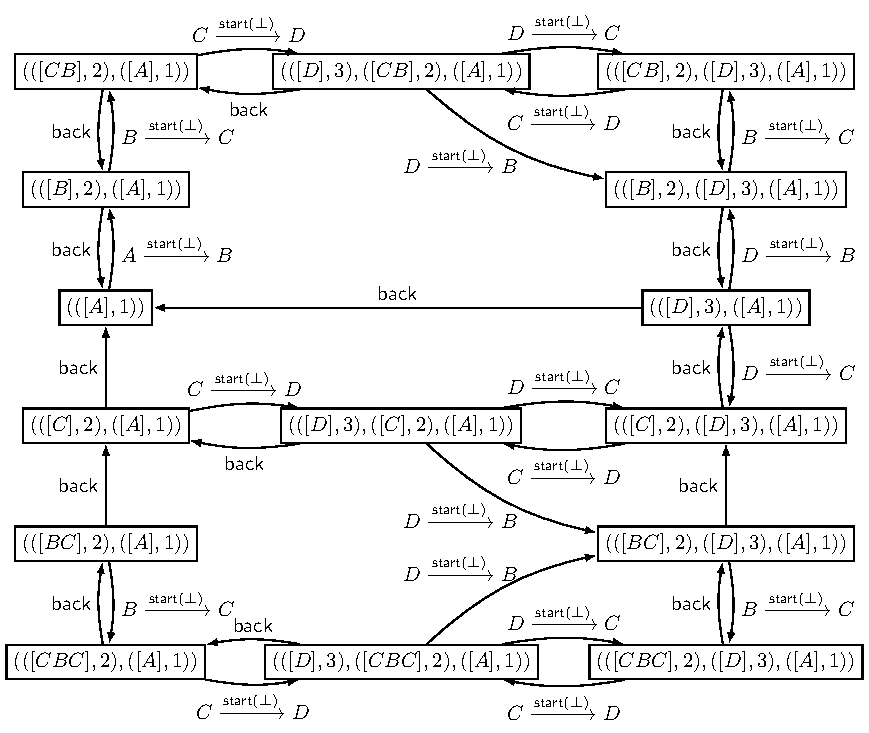
\includegraphics[scale = 0.75]{lmasm-example.pdf}
			\caption{Configurations reachable from the initial configuration $(([A], 1))$ in the $\LMAMASS$ $\Mm$}
				%in $\phi$
		% \vspace{-6mm}	
		\label{lmasm-example}
	\end{figure}
\end{example}

% Intuitively, $\STD$ is similar to $\STP$, without considering the case where $\lmd(A) = \SIT$, when a $\STD$ activity $B$ is started, it is directly pushed into the top task. 
% Recall that $\STP$ is shorthand of SingleToP, when a $\STP$ activity $B$ is started, it is pushed into the top task if the top activity of the top task is \emph{not} $B$.

% $\SIT$ is similar to $\STK$, for each $\SIT$ (resp. $\STK$) activity $B$, it can appear at most once in the configuration. However, they still have differences. Recall that $\SIT$ is shorthand for SingleInsTance, that means the task which $\SIT$ activity located has only one activity. This also explains why starting an $\STD$ or $\STP$ activity, it is \emph{not} pushed into the current task when the callee activity is an $\SIT$ activity.
% Moreover, when starting an activity $B$, if $\lmd(B)\in\{\STK,\SIT\}$ or the callee activity is the $\SIT$ activity, the first step is to specify to which task it will be allocated, more precisely, is to find the task which has the same task affinity with the caller activity. If the task is not found, it will launch a new task $[B]$ on the top of the configuration, if such a task $S_i$ is found, then $S_i$ will be moved to the top task of the configuration, and
% \begin{itemize}
% 	\item if $\lmd(B) = \STD$, then it will directly pushed into $S_i$,
% 	\item if $\lmd(B) = \STP$, it is pushed into $S_i$ if the top activity of $S_i$ is \emph{not} $B$.
% 	\item if $\lmd(B) = \SIT$, then $S_i$ will not change,
% 	\item if $\lmd(B) = \STK$, then it will directly pushed into $S_i$ when $B\notin S_i$, it will poped until the top activity is $B$ otherwise,
% \end{itemize}

\subsection{Semantics of $\IFAMASS$}
% In this case, we only consider the intent flags.
%To define the semantics of $\IFAMASS$, we add some auxiliary functions and predicates. 


%To define the semantics of $\IFAMASS$, we adapt slightly the notion of configurations and the auxiliary functions and predicates. 

Let $\Mm$ be an $\IFAMASS$, namely, $\lmd(A) = \STD$ and $\aft(A) = \aft(A_0)$ for each activity $A$. As a result, there is only one task in each configuration and the task allocation mechanism can be ignored here. Therefore, a configuration here is simply a word $[A_1,\cdots,A_m]\in\act^+$. 
% there is only one task in $\IFAMASS$.

Before formally defining the semantics of $\Mm$, let us first describe the intuitions of the intent flags. 
We would like to warn that although the intuitions of these intent flags may help the readers to get some preliminary idea of their meanings, before diving directly into the formal semantics, they are nonetheless inaccurate, especially when different flags may interfere with each other.

\paragraph{Intuitions of the Intent flags.}  Let us explain the intuitions of the five intent flags in the sequel. 
\begin{itemize}
	\item The $\stpflag$ intent flag:  If it is set,  it has the same effect as starting an activity of the $\STP$ launch mode.
	\item The $\ctpflag$ intent flag:  If it is set, it will check for the existence of the started activity in the task. If the activity exists, then all the activities above the topmost occurrence of the started activity in the task will be removed. Otherwise, the started activity will be pushed into the task.
	\item The $\rtfflag$ intent flag:  If it is set, it will check for the existence of the started activity in the task. If the activity exists, then the topmost occurrence of this activity will be moved to the top of this task. Otherwise, the started activity will be pushed into the task.
	\item The $\ntkflag$ intent flag:  If it is set, it will look for an existing task to put the started activity according to the task allocation mechanism. If such a task exists, the task will be moved to the top and the started activity is pushed to the task, otherwise a new task is created to put this activity.
	\item The $\ctkflag$ intent flag:  It is usually used together with $\ntkflag$. If it is set, it will remove all the activities in the task and push the started activity to the task.
\end{itemize}
%Moreover, $\ntkflag$ will only affect $\ctkflag$ in $\IFAMASS$, since there is only one task in $\IFAMASS$, task allocation mechanism will always allocate the top task.

%To define the semantics of $\IFAMASS$, the concept of configuration is adapted from the definition of configuration for $\LMAMASS$ as follows: A configuration of $\Mm$ is encoded as $[A_1,\cdots,A_m]\in\act^+$.

%Then we introduce some additional and adapted auxiliary functions and predicates that are to be used in the formal semantics of $\IFAMASS$.\\
Moreover, we introduce some additional functions and predicates. 
%\emph{Auxiliary functions and predicates.} 
Let $\rho$ be a configuration with $\rho = [A_1,\cdots,A_m]$. Then
%We define the following auxiliary functions and predicates.
\begin{itemize}
	% \item $\topact(\rho) = A_1$, $\btmact(\rho) = A_m$,
%	\item $\push(\rho, B) = [B, A_1,\cdots,A_m]$,
%	\item $\Pop(\rho) = [A_2,\cdots,A_m]$,
	% \item $\mvacttop(\rho, B) = ([B]\cdot S_1'\cdot S_1'', S_2, \cdots, S_n)$, if $S_1=S_1'\cdot[B]\cdot S_1''$ with $S_1'\in (\act\setminus\{B\})^*$,
%	\item $\clrtop(\rho, B) = [A_j,\cdots,A_m]$, if $A_j = B$ for some $j\in[m]$ and $B\notin[A_1,\cdots,A_{j-1}]$,
	\item $\mvacttop(\rho, B) = [A_j,A_1,\cdots,A_{j-1},A_{j+1},\cdots A_m]$, if $A_j = B$ for some $j\in[m]$ and $B\notin[A_1,\cdots,A_{j-1}]$,
	\item $\clrtsk(\rho, B) = [B]$.
\end{itemize}
Intuitively $\mvacttop(\rho, B)$ is used for defining the semantics of $\rtfflag$, and $\clrtsk(\rho, B)$ is used for defining the semantics of $\ctkflag$.

We are ready to define the semantics of $\IFAMASS$, that is, the relation $\rho \xrightarrow[\Mm]{\tau} \rho'$.
Let $\rho = [A_1,\cdots,A_m]$ for some $m\ge 1$ be the current configuration and $A_1 = A$. 

If $\tau = \back$ then $\rho' = \pop(\rho)$.

Let us assume  $\tau = A\xrightarrow[]{\startactivity(\phi)}B$ in the sequel.

\begin{itemize}
    \item If $\phi\models\ctkflag\wedge\ntkflag$, then $\rho' = \clrtsk(\rho, B)$.
    \item Otherwise,
    \begin{itemize}
        \item if $\phi \models\ctpflag$ and $B \in \rho$, then $\rho' =\clrtop(\rho, B)$,
		\item otherwise,
		\begin{itemize}
			\item if $\phi \models \rtfflag$ and $B \in \rho$, then $\rho'=\mvacttop(\rho, B)$,
			\item otherwise,
			\begin{itemize}
				\item if $\phi \models \stpflag$ and $A = B$, then $\rho' = \rho$,
				\item otherwise, $\rho' = \push(\rho, B)$.
			\end{itemize}
		\end{itemize}
    \end{itemize}
\end{itemize}
Let us use the following example to illustrate the semantics.
\begin{example}
	Let $\Mm = (\act,A,\lmd,\aft,\Delta)$ be an $\IFAMASS$, where $\act = \{A,B,C,D\}$, where for each $A'\in\act$, $\lmd(A') = \STD$ and $\aft(A') = 1$. 
	Moreover, $\Delta = \{\tau_1, \tau_2, \tau_3, \tau_4, \tau_5, \tau_6\}$, where 
		% $\rho_0 = (([D_1],D_1,1))$, and\
			$\tau_1 = A \xrightarrow{\startactivity(\ctkflag)} B$,
			$\tau_2 = B \xrightarrow{\startactivity(\rtfflag)} C$,
			$\tau_3 = C \xrightarrow{\startactivity(\ctpflag)} B$,
			$\tau_4 = C \xrightarrow{\startactivity(\rtfflag)} B$,
			$\tau_5 = C \xrightarrow{\startactivity(\ntkflag\wedge\ctkflag)} D$,
			$\tau_6 = D \xrightarrow{\startactivity(\stpflag)} D$.
	Then the configurations that are reachable from the initial configuration $[A]$ by executing the transition rules from $\Delta$ are illustrated in Figure~\ref{ifasm-example}, where the vertices denote the configurations and the edges denote the elements of $\xrightarrow[\Mm]{}$. 
	For instance, 
	\begin{itemize}
	\item if $A \xrightarrow{\startactivity(\ctkflag)} B$ is applied to the configuration $[A]$, then $B$ is pushed, since $\phi\models\neg\ntkflag \wedge \neg \ctpflag \wedge \neg \rtfflag \wedge \neg \stpflag$, resulting to the configuration $[BA]$,
	%
	\item if $B \xrightarrow{\startactivity(\rtfflag)} C$ is applied to the configuration $[BA]$, then $C$ is pushed, since $\phi\models\rtfflag$ and $C$ does not occur in the task $[BA]$, resulting to the configuration $[CBA]$,
	%
	\item if $C \xrightarrow{\startactivity(\ctpflag)} B$ is applied to the configuration $[CBA]$, then all the activities above $B$, which is $C$ here, are removed from the task, since $\phi\models\ctpflag$ and $B$ occurs in the task $[CBA]$, resulting to the configuration $[BA]$,
	%
	\item if $C \xrightarrow{\startactivity(\rtfflag)} B$ is applied to the configuration $[CBA]$, then $B$ is moved to the top of the task, since $\phi\models\rtfflag$ and $B$ occurs in the task $[CBA]$, resulting to the configuration $[BCA]$,
	%
	\item if $B \xrightarrow{\startactivity(\rtfflag)} C$ is applied to the configuration $[BCA]$, then $C$ is moved to the top of the task, since $\phi\models\rtfflag$ and $C$ occurs in the task $[BCA]$, resulting to the configuration $[CBA]$,
	%
	\item if $C \xrightarrow{\startactivity(\ntkflag\wedge\ctkflag)} D$ is applied to the configuration $[CBA]$, then all activities are removed from the task and $D$ is pushed, since $\phi\models\ntkflag\wedge\ctkflag$, resulting to the configuration $[D]$,
	%
	\item if $D \xrightarrow{\startactivity(\stpflag)} D$ is applied to the configuration $[D]$, then $D$ is not pushed, since $\phi\models\stpflag$ and $D$ is the top activity of the task, resulting to the configuration $[D]$.
	\end{itemize}
	Note that for $\Mm$, there are only finitely many configurations reachable from the initial configuration, which may not be the case for $\IFAMASS$ in general.  
		% $(([D_1],D_1,1))$\\
		% $\xrightarrow[\tau_1]{\Mm}(([P_1D_1],D_1,1))$\\
		% $\xrightarrow[\tau_2]{\Mm}(([P_1D_1],D_1,1))$\\
		% $\xrightarrow[\tau_3]{\Mm}(([K_2],K_2,0),([P_1D_1],D_1,1))$\\
		% $\xrightarrow[\tau_4]{\Mm}(([D_1K_2],K_2,0),([P_1D_1],D_1,1))$\\
		% $\xrightarrow[\tau_5]{\Mm}(([T_2],T_2,0),([D_1K_2],K_2,0),([P_1D_1],D_1,1))$\\
		% $\xrightarrow[\tau_6]{\Mm}(([K_2],K_2,0),([T_2],T_2,0),([P_1D_1],D_1,1))$\\
		
	
		
	\begin{figure}
		% \vspace{-3mm}
			\centering
			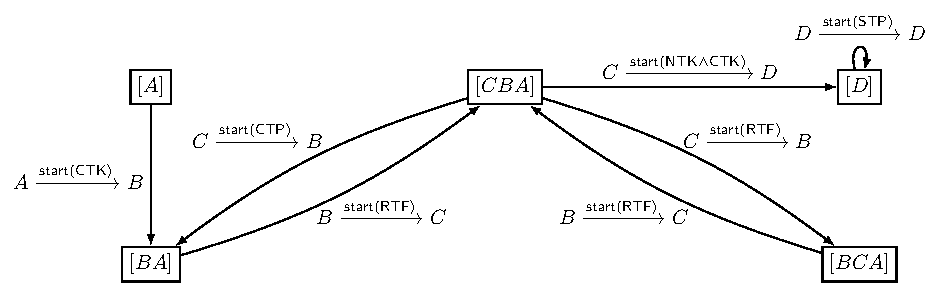
\includegraphics[scale = 0.75]{ifasm-example.pdf}
			\caption{Configurations reachable from the initial configuration $[A]$ in an $\IFAMASS$ $\Mm$}
				%in $\phi$
		% \vspace{-6mm}	
		\label{ifasm-example}
	\end{figure}
\end{example}
% In this case, we assume that the launch modes of activities are $\STD$.  Intuitively, for a transition $A\xrightarrow{\startactivity(\phi)}B$, the intent flags in $\phi$ may depend on each other. The dependency can exhibit in the following two forms: (1) $n$ \emph{subsumes} $n'$, i.e., $n'$ is ignored if $n$ co-occurs with $n'$, and the ``subsume'' relations are transitive, (2) $n$ \emph{enables} $n'$, i.e., $n'$ takes effect if $n$ co-occurs with $n'$. We summarize the dependencies among the intent flags in Figure xxx, 

% For a transition $A\xrightarrow{\startactivity(\phi)}B$, we conclude that :
% \begin{itemize}
% 	\item when $\ctkflag$ tasks effect, then the task will be cleared, and $B$ is pushed into the task,
% 	\item when $\ctpflag$ tasks effect, then the task will be poped until the top activity is $B$ when $B$ is in the task, $B$ will be pushed into the task otherwise, which is similar with the case $\lmd(B) = \STK$,
% 	\item when $\rtfflag$ tasks effect, then $B$ is escalated to the top of the task when $B$ is in the task, $B$ will be pushed into the task otherwise, 
% 	\item when $\stpflag$ tasks effect, then $B$ is pushed into the task when the top activity of the task is not $B$, which is similar with the case $\lmd(B) = \STP$.
% \end{itemize}

\subsection{Semantics of $\AMASS$}
%To define the semantics of $\AMASS$, we use the same definition of configuration as $\LMAMASS$, and add some auxiliary functions and predicates. 

Let $\Mm$ be an $\AMASS$. For clarity, in the sequel, we restate the aforementioned functions $\mvacttop$ and $\clrtsk$ for the configurations that may contain multiple tasks. 
%\emph{Auxiliary functions and predicates.} 
Let $\rho = ((S_1,\aname_1),\cdots, (S_n,\aname_n))$ be a configuration.
Then
\begin{itemize}
	\item $\mvacttop(\rho, B) = (([B]\cdot S_1'\cdot S_1'',\aname_1), (S_2,\aname_2), \cdots, (S_n,\aname_n))$, if $S_1=S_1'\cdot[B]\cdot S_1''$ with $S_1'\in (\act\setminus\{B\})^*$,
	\item $\clrtsk(\rho, B) = (([B],\aname_1), (S_2,\aname_2), \cdots, (S_n,\aname_n))$.
\end{itemize}
% In this case, we consider the launch modes, task affinities and intent flags.
Now we define the semantics of $\AMASS$. 

The semantics of the transition rule $\tau = \back$ is similar to that of $\LMAMASS$.

Let us  assume $\tau = A\xrightarrow[]{\startactivity(\phi)}B$ in the sequel.

Let $\rho = ((S_1,\aname_1),\cdots,(S_n,\aname_n))$ be the current configuration for some $n \ge 1$ and $\topact(\rho) = A$. Moreover, let $S_1 = [A_1',\cdots,A_m']$. Evidently, $A = A_1'$.

\medskip

\noindent \fbox{\fbox{$\lmd(B) = \standard$}}
\begin{itemize}
	\item If $\lmd(A) \neq \singleinstance$ and $\phi \models \neg \ntkflag$, 
	\begin{itemize}
        \item if $\phi \models\ctpflag$ and $B \in \toptsk(\rho)$, then $\rho' =\clrtop(\rho, B)$,
		\item otherwise,
		\begin{itemize}
			\item if $\phi \models \rtfflag$ and $B \in \toptsk(\rho)$, then $\rho'=\mvacttop(\rho, B)$,
			\item otherwise,
			\begin{itemize}
				\item if $\phi \models \stpflag$ and $B = \topact(\rho)$, then $\rho' = \rho$,
				\item otherwise, $\rho' = \push(\rho, B)$.
			\end{itemize}
		\end{itemize}
	\end{itemize}
	%
	\item If $\lmd(A) = \singleinstance$ or $\phi \models \ntkflag$, then
	\begin{itemize}
		\item if $\gettsk(\rho, B) = S_i$ for some $i\in[n]$,
		\begin{itemize}
            \item if $\phi \models\ctkflag$, then $\rho' = \clrtsk(\mvtsktop(\rho, i), B)$,
			\item otherwise, 
			\begin{itemize}
				\item if $\phi \models\ctpflag$ and $B \in S_i$, then $\rho' =\clrtop(\mvtsktop(\rho, i), B)$,
				\item otherwise,
				\begin{itemize}
					\item if $\phi \models \rtfflag$ and $B \in S_i$, then $\rho'=\mvacttop(\mvtsktop(\rho, i), B)$,
					\item otherwise,
					\begin{itemize}
						\item if $\phi \models \stpflag$ and $B = \topact(S_i)$, then $\rho' = \mvtsktop(\rho, i)$,
						\item otherwise, $\rho'=\push(\mvtsktop(\rho, i), B)$,
					\end{itemize}
				\end{itemize}
			\end{itemize}
		\end{itemize}
		\item if $\gettsk(\rho, B) = *$, then $\rho' = \newtsk(\rho, B)$.
	\end{itemize}
\end{itemize}

\noindent \fbox{\fbox{$\lmd(B) = \STP$}}
\begin{itemize}
	\item If $\lmd(A) \neq \singleinstance$ and $\phi \models \neg \ntkflag$, 
	\begin{itemize}
        \item if $\phi \models\ctpflag$ and $B \in \toptsk(\rho)$, then $\rho' =\clrtop(\rho, B)$,
		\item otherwise,
		\begin{itemize}
			\item if $\phi \models \rtfflag$ and $B \in \toptsk(\rho)$, then $\rho'=\mvacttop(\rho, B)$,
			\item otherwise,
			\begin{itemize}
				\item if $B = \topact(\rho)$, then $\rho' = \rho$,
				\item otherwise, $\rho' = \push(\rho, B)$.
			\end{itemize}
		\end{itemize}
	\end{itemize}
	%
	\item If $\lmd(A) = \singleinstance$ or $\phi \models \ntkflag$, then
	\begin{itemize}
		\item if $\gettsk(\rho, B) = S_i$ for some $i\in[n]$,
		\begin{itemize}
            \item if $\phi \models\ctkflag$, then $\rho' = \clrtsk(\mvtsktop(\rho, i), B)$,
			\item otherwise, 
			\begin{itemize}
				\item if $\phi \models\ctpflag$ and $B \in S_i$, then $\rho' =\clrtop(\mvtsktop(\rho, i), B)$,
				\item otherwise,
				\begin{itemize}
					\item if $\phi \models \rtfflag$ and $B \in S_i$, then $\rho'=\mvacttop(\mvtsktop(\rho, i), B)$,
					\item otherwise,
					\begin{itemize}
						\item if $B = \topact(S_i)$, then $\rho' = \mvtsktop(\rho, i)$,
						\item otherwise, $\rho'=\push(\mvtsktop(\rho, i), B)$,
					\end{itemize}
				\end{itemize}
			\end{itemize}
		\end{itemize}
		\item if $\gettsk(\rho, B) = *$, then $\rho' = \newtsk(\rho, B)$.
	\end{itemize}
\end{itemize}

\noindent \fbox{\fbox{$\lmd(B) = \STK$}}
\begin{itemize}
	\item If $\gettsk(\rho, B) = S_i$ for some $i\in[n]$,
	\begin{itemize}
		\item if $\phi \models\ctkflag$, then $\rho' = \clrtsk(\mvtsktop(\rho, i), B)$,
		\item otherwise, 
		\begin{itemize}
			\item if $B \notin S_i$, then $\rho' = \push(\mvtsktop(\rho, i), B)$,
			\item if $B \in S_i$, then $\rho' = \clrtop(\mvtsktop(\rho, i), B)$.
		\end{itemize}
	\end{itemize}
	\item If $\gettsk(\rho, B) = *$, then $\rho' = \newtsk(\rho, B)$.
\end{itemize}
\noindent \fbox{\fbox{$\lmd(B) = \SIT$}}
\begin{itemize}
	\item If $\gettsk(\rho, B) = S_i$ for some $i \in [n]$, then $\rho' = \mvtsktop(\rho, i)$,
	\item If $\gettsk(\rho, B) = *$, then $\rho' = \newtsk(\rho, B)$.
\end{itemize}




%===================================================================================================
% \section{Doubly-Nested Stack Systems} \label{sec:dnss}

% In this section, we introduce the model of Doubly-Nested Stack Systems (\DNSS).  
\begin{definition}[Doubly-Nested Stack Systems] \label{def:eps}
    A {\DNSS} is a tuple $\Dd = (\Gamma,\Gamma_\STK, \gamma_{\init}, \Delta)$, where $\Gamma$ is a finite stack alphabet with $\gamma_\init\in \Gamma$, and $\Delta \subseteq \{\POP\} \cup \Gamma \times \opset$ is the transition relation with 
    $\opset=\{\opn(\gamma)\mid \opn \in \{\PUSH, \STP, \CTP, \RTF\}, \gamma \in \Gamma\setminus\Gamma_\STK \} \cup \{\STK(\gamma)\mid \gamma\in\Gamma_\STK\}$. Moreover, it is required that $\POP \in \Delta$. (Intuitively, the $\POP$ operation can be applied anytime.)
	%\cup \Gamma \cup\{\back\}$
\end{definition}

%--------------------------------------------------------
Intuitively, a {\DNSS} specifies the evolution of a stack of stacks. Inspired by the Android multitasking mechanism, the lower-level stacks are referred to as \emph{tasks} and the upper-level stack, possibly comprising multiple tasks, is referred to as the \emph{task stack}. More formally, a task $S$ is an element of $\Gamma^*$, i.e., a sequence of symbols from $\Gamma$, with the leftmost symbol representing the top of the task; A task stack $\rho$ is of the form $(S_1,\cdots, S_n)$, where each $S_i$ is a task and $S_1$ is the topmost task. When necessary we use $\emptybackstack$ to denote an empty task stack, i.e., when $n=0$.

To precisely define the semantics of a {\DNSS}, we need some additional machinery. We assume that there is a finite \emph{name space} $\namespace$ such that each task $S$ is associated with a \emph{name} $\namefun(S)\in \namespace$. 
%
%Notice that the concrete definition will be given when a concrete system is instantiated. 
We assume that the name $\namefun(S)$ is determined when the task $S$ is created (i.e., being pushed into the task stack as a new task). Therefore, the name function $\namefun$ can also be seen as a function from $\Gamma$ to $\namespace$, that is, it maps from the first symbol of the task (which is pushed into the task when it is created) to some name in $\namespace$. 
%
Throughout  this paper we will insist this variant of $\namefun$. 
%\zhilin{add this explanation of $\namefun$.} 
Notice that distinct tasks may share the same name. Concrete definitions of the name space $\namespace$ and the name function $\namefun$ vary and are largely domain-specific. For instance, in the {\DNSS} dedicated to the Android multitasking mechanism,  the name of a task is defined as a pair $(A, s)$, where $A$ is the first \emph{activity} of the task when it is launched (this is called \emph{real activity} of the task) and $s$ is the \emph{task affinity} of $A$; we defer the detailed explanations to Section~\ref{sec:asm}.  

In \DNSS, a task stack $\rho=(S_1, \cdots, S_n)$ encompasses multiple tasks. When an operation $o \in \opset$ is to be executed, a distinguished feature of the {\DNSS} model---different from most of the other models based on pushdown systems---is that $\opset$ is not necessarily applied to the top task $S_1$, but may be applied to some task $S_i$ for $1<i\leq n$, depending on the names of all $S_i$'s given by the name function $\namefun$.\footnote{Readers might have already noticed that some operations in $\opset$, i.e., $\PUSH, \STP, \CTP, \RTF$, have two version with one being annotated with the @ symbol. The operation with @ is applied to the top task directly, while the one with @ needs to invoke the addressing mechanism.} To this end, we 
need to define an \emph{addressing} mechanism, i.e., to prescribe to which task the operation $o$ should be applied. In \DNSS, there are two possibilities: either a task is located to which $\op$ is then applied, or no task can be selected in which case a new task must be created. 

%given a sequence (stack) of stacks and $\gamma\in \Gamma$, which stack is to be operated? In our model,  
We consider an addressing mechanism which bases the decision on the word $\namefun(S_1)\cdots \namefun(S_n) = \namefun(\gamma_1)\cdots \namefun(\gamma_n) \in \namespace^+$ (where for each $i \in [n]$, $\gamma_i$ is the first symbol pushed to the task $S_i$ when $S_i$ was created) and the stack symbol $\gamma$ contained in $\opn(\gamma) \in \opset$ or $\opn^\addr(\gamma) \in \opset$. Formally, we define $(\alpha_\gamma)_{\gamma\in \Gamma}$, where % for each $\gamma\in \Gamma$, there is an addressing 
each function $\alpha_\gamma: \namespace^+\rightarrow \natnum\cup\{\bot\}$  is subject to the following two conditions, viz.  
\begin{itemize} 
	\item[(a)] $\alpha_\gamma(w)\in [|w|]\cup\{\bot\}$,  and 
	\item[(b)] for each $w \in \namespace^+$, $\namefun(\gamma)$ occurs in  $w$ entails that $\alpha_\gamma(w) \neq \bot$. 
\end{itemize}
%\zhilin{add this condition to guarantee that the number of tasks is bounded when $\LTK$ is missing. }. 
%In case that $\alpha_\gamma(w)$ returns the index of the lower-level stack in the upper-level stack that will be operated, or otherwise---in case of returning $\bot$, a new lower-level stack will be created. 
As mentioned, concrete definitions of $(\alpha_\gamma)_{\gamma\in \Gamma}$ vary; for the Android multitasking mechanism, %Concretely, the addressing machinery, i.e., $\alpha_\gamma$ is 
we shall employ an automata model (tentative: Cost Register Automata, CRA). 

\subsection{Semantics}

As usual, we define the semantics of {\DNSS} as a transition system over configurations.
Configuration of {\DNSS} $\Dd$ are task stacks which are encoded as $\rho=(S_1,\cdots, S_n)$
with $S_i = [\gamma_{i,1}, \cdots, \gamma_{i, m_i}]$ for each $i \in [n]$. We define $\topact(\rho):=\gamma_{1,1}$. The \emph{initial} configuration is $([\gamma_{\init}])$ which contains one task $[\gamma_\init]$ only. The \emph{height} of a configuration $\rho$ is defined as the maximum height of tasks in $\rho$.
%As usual, the semantics of {\DNSS} is defined as 
The transition relation is denoted by $\rightarrow_{\Dd}$, defined in the sequel.  %over the set of all configurations. Namely, 
\begin{itemize}
\item $\POP \in \Delta$ induces the transitions $\rho\rightarrow_\Dd \rho'$ such that one of the following two conditions holds,
\begin{itemize}
\item  $\rho = (S_1, S_2, \cdots, S_n)$ and $\rho' = (S'_1, S_2, \cdots, S_n)$, $S_1 = [\gamma_{1, 1}, \cdots, \gamma_{1, m_1}]$ with $m_1 \ge 2$, and $S_1' = [\gamma_{1, 2}, \cdots, \gamma_{1, m_1}]$, 
%
\item $\rho = (S_1, S_2, \cdots, S_n)$, $S_1 = [\gamma_{1,1}]$, and $\rho' = (S_2, \cdots, S_n)$.
\end{itemize}
Note that the $\POP$ operation does not depend on the top symbol, thus can be applied anytime.

\item Each $(\gamma, o)\in \Delta$ induces transitions $\rho\rightarrow_\Dd \rho'$ with $\topact(\rho)=\gamma$. We now define the effect of the operation $o\in \opset$ on $\rho$, i.e., the resulting $\rho'$. 
    Recall that $\opset=\{\opn(\gamma)\mid \opn \in \{\PUSH, \STP, \RTF, \CTP\}, \gamma \in \Gamma\setminus\Gamma_\STK \} \cup \{\STK(\gamma)\mid \gamma\in\Gamma_\STK\}$.
\begin{itemize}
	\item $\PUSH(\gamma)$. This operation is similar to the push operation in traditional pushdown systems, namely, $\gamma$ is simply pushed into the top task $S_1$ where no addressing mechanism is needed.	 
  	\item $\STP(\gamma)$. This is a shorthand for ``\textbf{S}ingle \textbf{T}o\textbf{P}''. It is the same as $\PUSH(\gamma)$, except that if $\gamma$ is already the top of $S_1$ then $\gamma$ is \emph{not} pushed into $S_1$ (and thus $\rho':=\rho$). 
%-------------------------------------------------------------------------------------------------------
	\item $\RTF(\gamma)$. This is a shorthand for ``\textbf{R}eorder \textbf{T}o \textbf{F}ront". If $\gamma$ occurs in $S_1$ whereby $S_1=[\gamma_{1,1}, \cdots, \gamma_{1,m_1}]$ with $\gamma_{1,j} =\gamma$ for some $j \in [m_1]$  and $\gamma_{1, j'} \neq \gamma$ for all $j': 1 \le j' < j$. Then $\RTF(\gamma)$ escalates $\gamma_{1,j}$ to be the top of $S_1$, resulting in  
	$\widetilde{S_1} = [\gamma_{1,j}, \gamma_{1,1}, \cdots, \gamma_{1,j-1}$, $\gamma_{1,j+1}, \cdots, \gamma_{1,m_1}]$.
	Otherwise, $\gamma$ does not occur in $S_1$, then $\RTF(\gamma)$ pushes $\gamma$ into $S_1$, resulting in $\widetilde{S_1} = [\gamma, \gamma_{1,1}, \cdots, \gamma_{1,m_1}]$. In either case,  $\rho':=(\widetilde{S_1}, S_2, \cdots, S_n)$.
%----------------------------------------------------------------------------------------
	
	\item $\CTP(\gamma)$. This is a shorthand for ``\textbf{C}lear \textbf{T}o\textbf{P}". Suppose $\gamma$ occurs in $S_1$ whereby $S_1=[\gamma_{1,1}, \cdots, \gamma_{1,m_1}]$ with $\gamma_{1,j} =\gamma$ for some $j \in [m_1]$ and $\gamma_{1,j'} \neq \gamma$ for all $j': 1 \le j' < j$. Then $\CTP(\gamma)$ removes all the symbols on top of $\gamma_j$ from $S_1$, resulting in $\widetilde{S_1} = [\gamma_{1,j}, \cdots, \gamma_{1,m_1}]$; %keep the other tasks of $\rho$ unchanged. 
%
Otherwise $\gamma$ does not occur in $S_1$, then $\CTP(\gamma)$ pushes $\gamma$ into $S_1$, resulting in $\widetilde{S_1} := [\gamma, S_1]$. In either case, $\rho':=(\widetilde{S_1}, S_2, \cdots, S_n)$.  
%-------------------------------------------------------------------------------------
\item $\STK(\gamma)$. This is a variant of the $\CTP$ operation with addressing. 
	 If $\alpha_\gamma$ returns $i \in [n]$, then $\STK(\gamma)$ first escalates $S_i$ to be top task of the task stack, resulting in $\rho''=(S_i, S_1, \cdots, S_{i-1}, S_{i+1}, \cdots, S_n)$, and then applies the operation $\CTP(\gamma)$ to $\rho''$ to obtain $\rho'$. 	 
	 Otherwise, $\alpha_\gamma$ returns $\bot$, then a new task $S'=[\gamma]$ is created and $\rho':=(S', S_1, \cdots, S_n)$.
%-------------------------------------------------------------------------------------
\end{itemize}
We will use $\rightarrow_\Dd^*$ to denote the reflexive and transitive closure of $\rightarrow_\Dd$.

\paragraph{Reachability problem} Given a $\DNSS$ $\Dd$ and a configuration $\rho = (S_1, \cdots, S_n)$, decide whether $\rho$ is reachable from the initial configuration in $\Dd$.
\end{itemize}







%===================================================================================================
% \section{Pushdown systems with well-partially-ordered transductions} \label{sec:wpotrpds}

% 
% Recall that the definition of $\STK$-dominating $\IFAMASS$, then we let $\tau= A\xrightarrow{\startactivity(\bot)}B$ and let $\rho = (S_1, \cdots, S_n)$ be the current configuration for some $n \ge 1$ and $\topact(\rho) = A$,  we define the semantics of $\STK$-dominating $\IFAMASS$ as follows:
% \begin{itemize}
% 	\item If $\phi \models\ctpflag$ and $B \in \toptsk(\rho)$, then $\rho' =\clrtop(\rho, B)$,
% 	\item Otherwise,
% 	\begin{itemize}
% 		\item if $\phi \models \rtfflag$ and $B \in \toptsk(\rho)$, then $\rho'=\mvacttop(\rho, B)$,
% 		\item otherwise,
% 		\begin{itemize}
% 			\item if $\phi \models \stpflag$ and $B = \topact(\rho)$, then $\rho' = \rho$,
% 			\item otherwise, $\rho' = \push(\rho, B)$.
% 		\end{itemize}
% 	\end{itemize}
% \end{itemize}
In this case, there is only one task in $\Mm$, our approach to tackle this case is to simulate $\Mm$ by an extension of {\TrPDS}, i.e., pushdown systems with well-partially-ordered transductions ({\WOTrPDS}). In {\WOTrPDS}, the closure of transductions admits a basis which is well-partially-ordered with respect to the superset relation.
Theorem~\ref{thm-wstrpds-reach} shows the regular reachability problem of {\WOTrPDS} is decidable and Section~\ref{sec-proof-reach} proves the configuration reachability problem of $\STK$-dominating $\AMASS$ in this case is decidable.

Recall that there are four behaviors of $\Mm$ in this case, i.e., $\push$, $\mvacttop$, $\clrtop$ and $\Pop$.
The basic idea is to simulate the behaviorss of $\Mm$ by the transition rules of a {\TrPDS}. While it is relatively easy to simulate the behaviors $\push, \clrtop, \Pop$, %by the transition rules of $\Pp_\Aut$, 
it is challenging to simulate $\mvacttop$. Given a transition $A\xrightarrow{\startactivity(\phi)}B$ with $\phi\models\rtfflag\wedge\neg\ctpflag$, the semantics requires to move the topmost occurrence of $B$ (if there is any) to the top of $\rho$. The most direct way to simulate it with $A \neq B$ is by two transition rules $p \xrightarrow{A / B | \tau_{B, A}} p$ and  $p \xrightarrow{A / BA | \tau_{\not B}} p$
%\jl{this should be $p \xrightarrow{A / BA | \tau_{\not B}} p$}
(where $p$ is a state in $\Pp_\Mm$), corresponding to the two situations that $B$ occurs/does no occur in the stack, where 
\begin{itemize}
\item $\tau_{B, A}$ is the transduction that removes the first occurrence of $B$ from the input string and adds $A$ in the beginning, and
%
\item $\tau_{\not B}$ checks that $B$ does not occur in the input string but keeps the input string unchanged. 
\end{itemize}

However, such a direct simulation would entail an \emph{infinite} transduction closure:
$\tau^n_{B, A}$  (where $n \ge 1$), i.e. the $n$-fold composition of $\tau_{B,A}$, is the transduction that removes the first $n$ occurrences of $B$ from the input string and add $n$ $A$'s in the beginning. 
Therefore, we could not use {\TrPDS} to simulate $\Mm$, 

\begin{definition}[Union-basis of transduction sets]\label{def-ubasis}
Let $\TranSet$ be a set of transductions and $\Tranbasis \subseteq \TranSet$. Then $\Tranbasis$ is called a \emph{union-basis} of $\TranSet$ if each $\tau \in \TranSet$ is equivalent to a finite union of transductions from $\Tranbasis$ (called a $\Tranbasis$-representation of $\tau$). 
%Moreover, if $\tau \in \TranSet$ is equivalent to $\tau_1 \cup \cdots \cup \tau_n$ with $\tau_i \in \Tranbasis$ for every $i \in [n]$, then $\tau_1 \cup \cdots \cup \tau_n$ is called a $\Tranbasis$-representation of $\tau$.
\end{definition}

%We are ready to define pushdown systems with well-partially-ordered transductions.
\begin{definition}[Pushdown systems with well-partially-ordered transductions, \WOTrPDS] \label{def:defatpds}
    A \emph{pushdown system with well-partially-ordered transductions} (\WOTrPDS) is a tuple $\Pp = (P, \Gamma, \TranSet, \Delta)$, 
    where $P$ is a finite set of $control\ states$, $\Gamma$ is a finite $stack\ alphabet$, $\TranSet \subseteq \UTrans$ is a finite set of letter-to-letter transductions, and $\Delta \subseteq P \times \Gamma \times \Gamma^{\le 2} \times \TranSet \times P$ is a finite set of transition rules, where $\Gamma^{\le 2} = \{\varepsilon\} \cup \Gamma \cup \Gamma \times \Gamma$. In other words, each transition in $\Delta$ is of one of the following forms, $(p, \gamma, \varepsilon, \tau, p')$, $(p, \gamma, \gamma',\tau, p')$, or $(p, \gamma, \gamma'_1 \gamma'_2, \tau, p')$ such that $\gamma, \gamma', \gamma'_1, \gamma'_2 \in \Gamma$ and $\tau \in \TranSet$. 
   Moreover, it is required that there is a union-basis $\Tranbasis \subseteq \langle \TranSet \rangle$ such that 
   \begin{itemize}
   \item $\{\emptyset, \tau_{\varepsilon}\} \subseteq \Tranbasis$,  (note here $\tau_{id}$ may not be in $\Tranbasis$)
   %
   \item  $(\Tranbasis, \preceq)$ is a wpo, namely, it satisfies DCC and does not contain infinite antichains, and
%
   \item for each $\tau \in \langle \TranSet \rangle$, a $\Tranbasis$-representation $\beta_\tau = \beta_{\tau, 1} \cup \cdots \cup \beta_{\tau, n_\tau}$ can be computed effectively, 
%
   \item $\preceq$ is union-distributive over $\Tranbasis$-representations, specifically, for each $\beta \in \Tranbasis$ and $\tau \in \langle \TranSet \rangle$ whose $\Tranbasis$-representation is $\beta_\tau=\beta_{\tau, 1} \cup \cdots \cup \beta_{\tau, n_\tau}$, if $\tau \preceq \beta$, then $ \beta_{\tau, i} \preceq \beta$ for some $i \in [n_\tau]$.
\end{itemize}
   % can be effectively rewritten as a finite union of transductions from $\Tranbasis$.
%   $(\langle \TranSet \rangle, \preceq)$ is a wpo, namely, it satisfies DCC and does not contain infinite antichains.
%The size of $\Pp$, denoted by $|\Pp|$, is defined as $|\Delta|$.
\end{definition}
For readability, we usually write a transition $(p, \gamma, w, \tau, p') \in \Delta$ as $p \xrightarrow{\gamma/w | \tau} p'$.

%Let $\Pp = (P, \Gamma, \TranSet, \Delta)$ be  a {\WOTrPDS}. 
A \emph{configuration} $c$ of $\Pp$ is a pair $(p, w)$, where $w = \gamma_1 \cdots \gamma_k \in \Gamma^*$ is the  stack content with $\gamma_1$ as the topmost symbol. We define a binary relation $\xrightarrow{\Pp}$ over the set of configurations as follows. Given two configurations $(p_1, w_1)$ and $(p_2, w_2)$, $(p_1, w_1) \xrightarrow{\Pp} (p_2, w_2)$ if $w_1 = \gamma w'_1$, and one of the following conditions holds,
\begin{itemize}
\item $p_1 \xrightarrow{\gamma/\varepsilon|\tau} p_2$ for some $\tau$ with  $w_2 \in \tau(w'_1)$, 
%
\item $p_1 \xrightarrow{\gamma/\gamma'|\tau} p_2$ for some $\gamma'$ and $\tau$ with $w_2 = \gamma' w'_2$ for some $w'_2 \in \tau(w'_1)$, 
%
\item $p_1 \xrightarrow{\gamma/\gamma' \gamma''|\tau} p_2$ for some $\gamma', \gamma''$ and $\tau$ with $w_2 = \gamma' \gamma'' w'_2$ for some $w'_2 \in \tau(w'_1)$.
\end{itemize}
Moreover, we use $\xRightarrow{\Pp}$ to denote the reflexive and transitive closure of $\xrightarrow{\Pp}$. We say that $(p_2, c_2)$ is \emph{reachable} from $(p_1, c_1)$ if $(p_1, c_1) \xRightarrow{\Pp} (p_2, c_2)$.
\begin{figure}[htb]
    \centering
	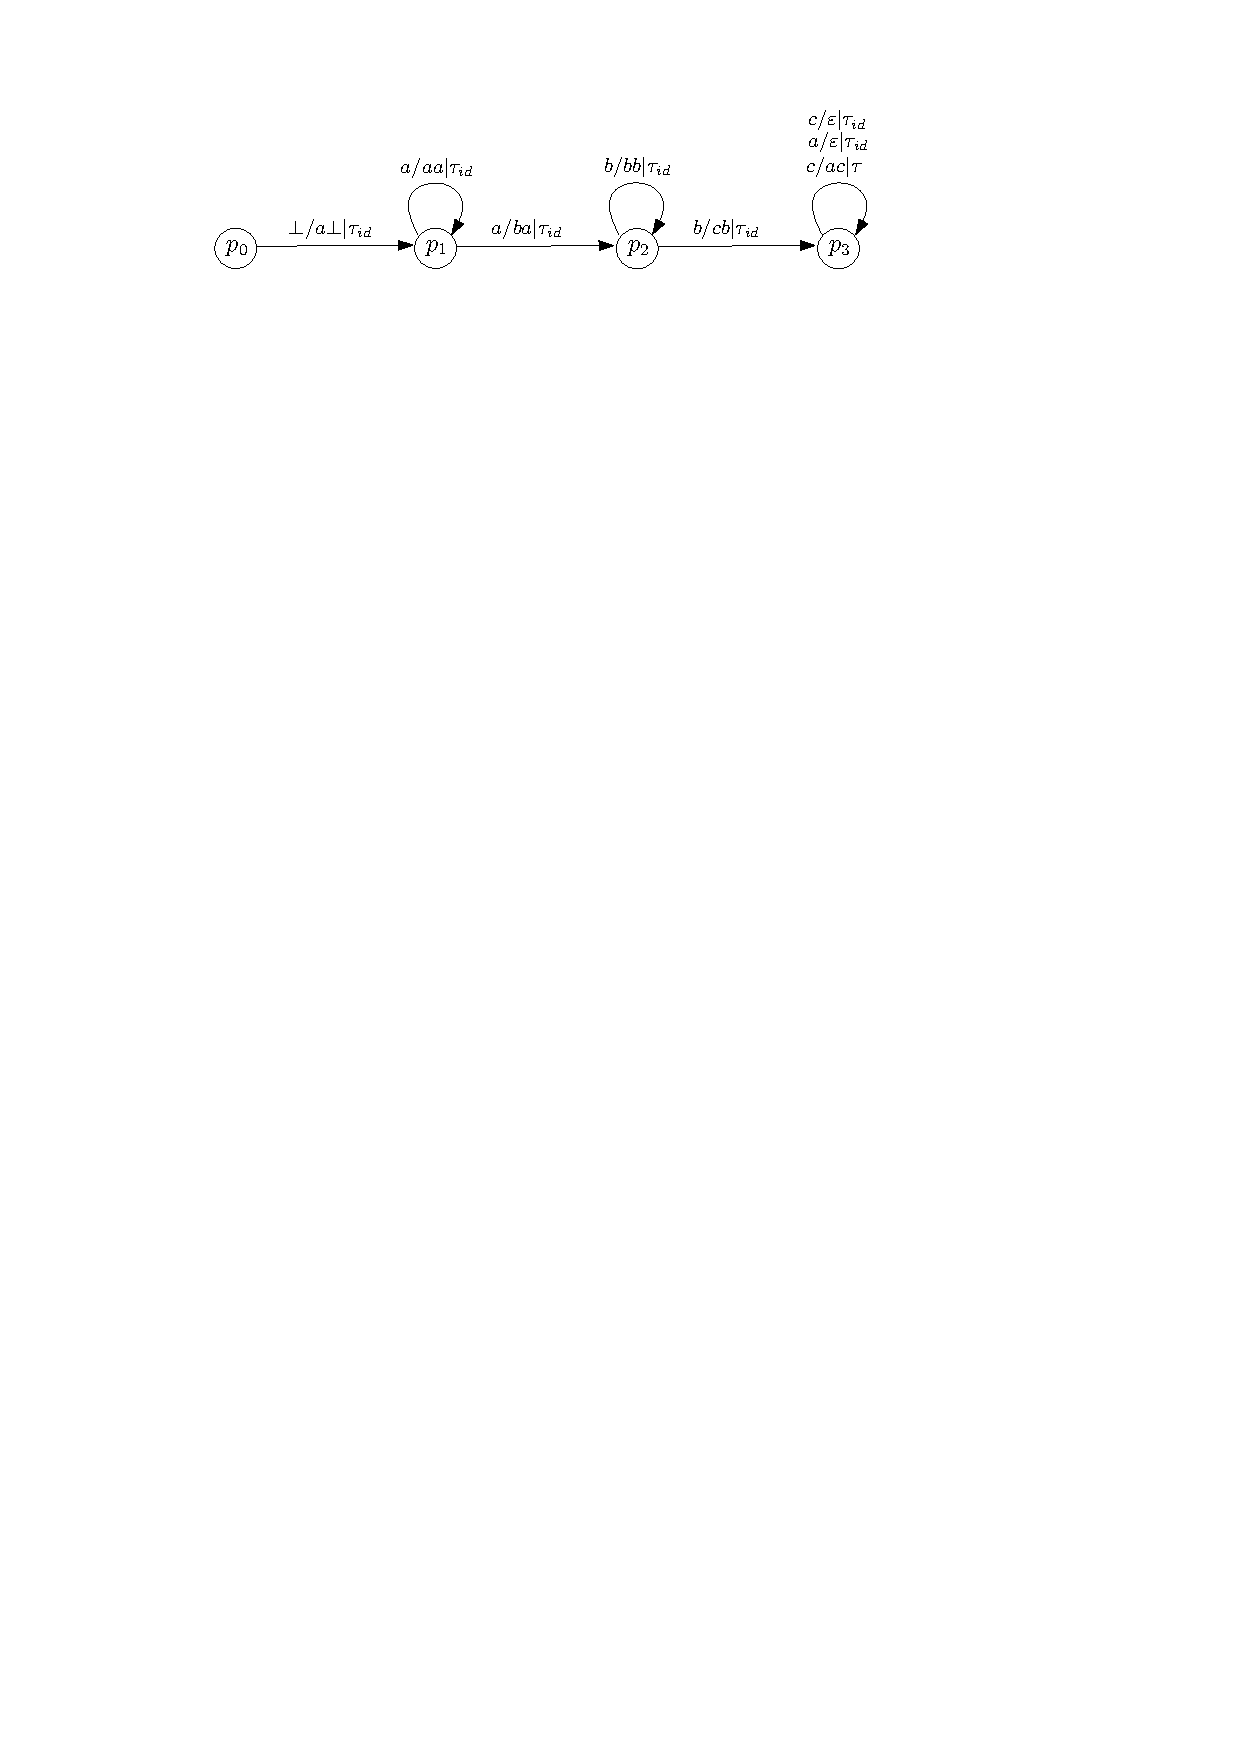
\includegraphics[scale = 0.9]{wstrpds-example.pdf}
	\caption{An example for \WOTrPDS}\label{fig-wstrpds-exmp}
\end{figure}

\begin{example}\label{exmp-wpotrpds}
Consider the {\WOTrPDS} $\Pp=(P, \Gamma, \TranSet, \Delta)$ (see Figure~\ref{fig-wstrpds-exmp}), where 
\begin{itemize}
\item $P = \{p_0, p_1, p_2, p_3\}$,  $\Gamma = \{\bot, a, b, c, d\}$,
% 
\item $\TranSet = \{\tau_{id}, \tau\}$, where $\tau$ is the transduction defined as follows: upon an input $w \in \Gamma^*$ where $a$ occurs at least once, it replaces at least the first occurrence of $a$ by $d$, more precisely, it nondeterministically chooses some $n \ge 1$ and replaces each of the first $n$ occurrences of $a$ in $w$ by $d$, for instance, $\tau(babad\bot) = \{bdbad\bot, bdbdd\bot\}$,
%
\item $\Delta$ is as illustrated in Figure~\ref{fig-wstrpds-exmp}, in particular, $(p_3, c, ac, \tau, p_3) \in \Delta$. 
%\left\{
%\begin{array}{l}
%(q_0, \bot, a\bot, \tau_{id}, q_1), (q_1, a, aa, \tau_{id}, q_1), (q_1, a, ba, \tau_{id}, q_2), (q_2, b, bb, \tau_{id}, q_2), \\
%(q_2, b, cb, \tau_{id}, q_3), (q_3, c, ac, \tau_1, q_3), (q_3, a, \epsilon, \tau_{id}, q_3) 
%\end{array}
%\right\}$.
\end{itemize}

From the definition of $\Delta$, $(p_3, bbdd\bot)$ is reachable from $(p_0, \bot)$, as witnessed by the following path in $\xrightarrow{\Pp}$, 
\[
\begin{array}{l}
(p_0, \bot) \xrightarrow{\Pp} (p_1, a \bot) \xrightarrow{\Pp} (p_1, aa \bot) \xrightarrow{\Pp} (p_2, baa \bot)  \xrightarrow{\Pp} (p_2, bbaa \bot)  \xrightarrow{\Pp} (p_3, cbbaa \bot)  \\
\xrightarrow{\Pp} (p_3, acbbdd \bot) \xrightarrow{\Pp} (p_3, cbbdd \bot)  \xrightarrow{\Pp} (p_3, bbdd \bot). 
\end{array}
\]
Note that, from the configuration $(p_3, cbbaa \bot)$, the transition $p_3 \xrightarrow{c/ac|\tau } p_3$ is applied. Then  $bbaa$ is transformed by $\tau$ into $bbdd$, moreover, $a$ is pushed. Therefore, the configuration $(p_3, acbbdd)$ is produced.

It is necessary to verify that $(\langle \TranSet \rangle, \preceq)$ has a well-partially-ordered union-basis $\Tranbasis$. First, we observe that $\tau^1 \supseteq \tau^2 \supseteq \cdots$, where $\tau^i$ for $i \ge 1$ is the $i$-fold composition of $\tau$, more specifically, $\tau^i$ nondeterministically replaces each of the first $n $ occurrences of $a$ in an input $w$ by $d$ for some $n \ge i$. It follows that $\tau^i \cup \tau^j = \tau^i$ for every $i < j$.
Moreover, $\lceil a, d \rfloor^{-1} \tau = \tau_{id} \cup \tau$. Therefore, the transduction closure $\langle \TranSet \rangle$ is $\{\emptyset, \tau_{id}, \tau_\varepsilon\} \cup \{\tau^i \mid i \ge 1\} \cup \{\tau_{\varepsilon} \cup \tau^i \mid i \ge 1\} \cup \{\tau_{id} \cup \tau^i \mid i \ge 1\}$. Let $\Tranbasis = \{\emptyset, \tau_{id}, \tau_\varepsilon\} \cup \{\tau^i \mid i \ge 1\}$. Then $\Tranbasis$ is a union-basis of $\langle \TranSet \rangle$. 
%, where $\tau^i$ is the $i$-fold composition of $\tau$, more specifically, $\tau^i$ nondeterministically replaces each of the first $n $ occurrences of $a$ in $w$ by $d$ for some $n \ge i$. 
%Note that $\tau_i$ is obtained as the $i$-fold composition of $\tau$. 
%
From $\tau^1 \supseteq \tau^2 \supseteq \cdots$, we deduce that each infinite descending chain of $(\Tranbasis, \preceq)$, i.e. each infinite ascending chain of $(\Tranbasis, \subseteq)$, eventually stabilizes at $\emptyset, \tau_{id}, \tau_\varepsilon$, or $\tau^i$ for some $i$. Thus $(\Tranbasis, \preceq)$ contains no infinite strictly descending chains, i.e. it satisfies the DCC condition. Moreover, from $\tau^1 \supseteq \tau^2 \supseteq \cdots$, we know that it contains no infinite antichains as well. We conclude that $(\Tranbasis, \preceq)$ is a wpo. The distributivity of $\preceq$ over $\Tranbasis$-representations is evident. \qed
%
%An example of {\WSTrPDS} here.
\end{example}

In this paper, we consider the \emph{regular reachability problem} of {\WOTrPDS}.
\begin{quote} 
	Given a {\WOTrPDS} $\Pp = (P, \Gamma, \TranSet, \Delta)$, control states $p_1, p_2 \in P$, regular languages $L_1, L_2$ over $\Gamma$, determine whether there exist %strings $w_1, w_2$ such that 
	$w_1 \in L_1$, $w_2 \in L_2$ such that $(p_1, w_1) \xRightarrow{\Pp} (p_2, w_2)$.
\end{quote}
%\begin{itemize}
%\item The \emph{reachability problem} is to check for two given configurations $(q_1, w_1)$ and $(q_2, w_2)$, whether $(q_1, w_1) \xRightarrow{\Pp} (q_2, w_2)$.
%
%\item 
%\end{itemize}

%We will show that the regular reachability problem of {\WOTrPDS} is decidable. In the next section, a model called finite automata with well-ordered transductions will be introduced, to represent sets of configurations of {\WOTrPDS}.


\begin{theorem}\label{thm-wstrpds-reach}
The regular reachability problem of {\WOTrPDS} is decidable.
\end{theorem}

Fix a  {\WOTrPDS} $\Pp = (P, \Gamma, \TranSet, \Delta)$. %and $\Aut = (Q, \Gamma, \delta, P, F)$ be a $\Pp$-{\NFA}. 
We show Theorem~\ref{thm-wstrpds-reach} via the saturation technique, which %by applying the saturation procedures from \cite{SM+15,Song18}. 
requires to represent the set of reachable configurations of $\Pp$. For traditional pushdown systems, a tailored {\NFA} (commonly referred to as P-automata in literature) suffices. For {\WOTrPDS}, we %generalize P-automata to 
introduce a new model, viz., \emph{finite automata with well-partially-ordered transductions} ({\WOTrNFA}), in Section~\ref{sec-wotrnfa}. 
Then in Section~\ref{sect:decidability}, we utilize the saturation technique to reduce the regular reachability problem of {\WOTrPDS} %the decidability % by reducing 
to the intersection problem of {\WOTrNFA} and {\NFA}, which is shown to be decidable in Section~\ref{sec:fatrnfa}.

We prove Theorem~\ref{thm:st-amass-reach} by showing that a {\WOTrPDS} $\Pp_\Mm = (P_\Mm, \Gamma_\Mm, \TranSet_\Mm, \Delta_\Mm)$ can be constructed from a given {\AMASS} $\Mm = (Act, A_0,\lmd,\aft,\Delta)$ to simulate the behaviors of $\Mm$. We show the details in Section~\ref{sec-proof-reach}


\subsubsection{Finite automata with well-partially-ordered transductions}\label{sec-wotrnfa}
 
\begin{definition}[Finite automata with well-partially-ordered transductions, {\WOTrNFA}] %[Finite automata with finite ascending chians and antichains transductions]
	Given a {\WOTrPDS} $\Pp=(P, \Gamma, \TranSet, \Delta)$ with $\Tranbasis$ as the union-basis of $\langle \TranSet \rangle$, a $\Pp$-{\WOTrNFA} is a tuple $\Aut =(Q, \Gamma, \delta, %P, 
	F)$,
	where $Q$ is the set of states such that $P \subseteq Q$, $F$ is the set of final states,  
	%and the set of initial states is $P$, %is a finite set of states, $\Sigma$ is a finite alphabet, 
	%$\TranSet$ is a finite set of transductions, %$I \subseteq Q$ (reps. $F \subseteq Q$) is a finite set of initial (reps. final) states, 
	and $\delta \subseteq Q \times \Gamma_\varepsilon \times \Tranbasis \times Q$ is a finite set of transition rules.

    A $\Pp$-{\WOTrNFA} $\Aut$ is called a {$\Pp$-{\NFA}} if for every $(q, a, \beta, q')$, $\beta = \tau_{id}$. 
\end{definition}

For convenience, we write a transition $(q, a, \beta, q')$ as $q \xrightarrow{a | \beta} q'$. 
To define the semantics of $\Aut$, we extend the transition rules $q \xrightarrow{a | \beta} q' \in \delta$  to a relation $q \xRightarrow{w | \tau} q'$ for a string $w$,  
%
%The relation $q \xRightarrow{w | \tau} q'$ is  
defined inductively as follows:
\begin{itemize}
	\item if $q \xrightarrow{a |\beta} q'$, then $q \xRightarrow{a | \beta} q'$, 
	%
	\item if $q \xRightarrow{w | \tau} q'$ and $q' \xrightarrow{b |\beta } q'' $, then $q \xRightarrow{w a | (\lceil a, b\rfloor^{-1}\tau) \circ \beta} q''$ for every $a \in \Gamma_\varepsilon$ such that $\lceil a, b\rfloor^{-1}\tau \neq \emptyset$.
\end{itemize}
Intuitively, $q \xRightarrow{w | \tau} q'$ means that in $\Aut$,  $q'$ is reached starting from $q$ after reading $w$. Moreover, the transduction $\tau$, which is  to be applied to the remaining suffix of the input string, is produced. Note that the transduction  $\tau \in \langle \TranSet \rangle$ in $q \xRightarrow{w | \tau} q'$ may not be in $\Tranbasis$. 

A configuration $(p, w)$ of $\Pp$ is accepted by $\Aut$ if $p \xRightarrow{w | \tau} q$ for some $q \in F$ and $\tau \in \langle \TranSet \rangle$ such that $(\varepsilon, \varepsilon) \in \tau$.
%
Let us use $\ConfSet(\Aut)$ to denote the set of configurations of $\Pp$ accepted by $\Aut$.

It turns out that $\Pp$-{\WOTrNFA} is capable of representing \emph{non-regular} set of configurations, as %witnessed 
shown by the following example.
\begin{example}
Let $\Pp$ be the {\WOTrPDS} in Example~\ref{exmp-wpotrpds}. Consider the $\Pp$-{\WOTrNFA} $\Aut = (Q, \Gamma, \delta, F)$ in Figure~\ref{fig-ptrnfa-exmp}, where $F= \{q_1\}$ and $\tau$ is the transduction from $\Pp$ that replaces at least the first occurrence of $a$ by $d$. From $p_3 \xrightarrow{c | \tau} p_3$, $p_3 \xrightarrow{b | \tau_{id}} q_1$, we have $p_3  \xRightarrow{c b | (\lceil b, b\rfloor^{-1} \tau) \circ \tau_{id}} q_1$, thus $p_3 \xRightarrow{cb | \tau} q_1$. Moreover, from $q_1 \xrightarrow{d | \tau_{id}} q_1$, we deduce $p_3 \xRightarrow{c b a | (\lceil a, d\rfloor^{-1} \tau) \circ \tau_{id}} q_1$. Since $(\lceil a, d\rfloor^{-1} \tau) \circ \tau_{id} = \tau_{id} \cup \tau$, we have $p_3 \xRightarrow{c b a |  \tau_{id} \cup \tau} q_1$ and $(\epsilon, \epsilon) \in \tau_{id} \cup \tau$. Thus $(p_3, cba)$ is accepted by $\Aut$. On the other hand, although $p_3 \xRightarrow{cb | \tau} q_1$ with $q_1 \in F$, but $(\epsilon, \epsilon) \not \in \tau$, thus $(p_3, cb)$ is not accepted by $\Aut$.  Furthermore, we observe that for $m \ge 1$, $p_3 \xRightarrow{c^m | \tau^m} p_3$. From the fact that $\tau^m$ replaces at least $m$ occurrences of $a$ by $d$, we deduce that for each configuration of the form $(p_3, c^m b a^n)$ with $m,n \ge 1$, it is accepted by $\Aut$ iff $n \ge m$.  Therefore, $\ConfSet(\Aut)$, the set of configurations accepted by $\Aut$, is non-regular. 
%
\begin{figure}[htb]
    \centering
	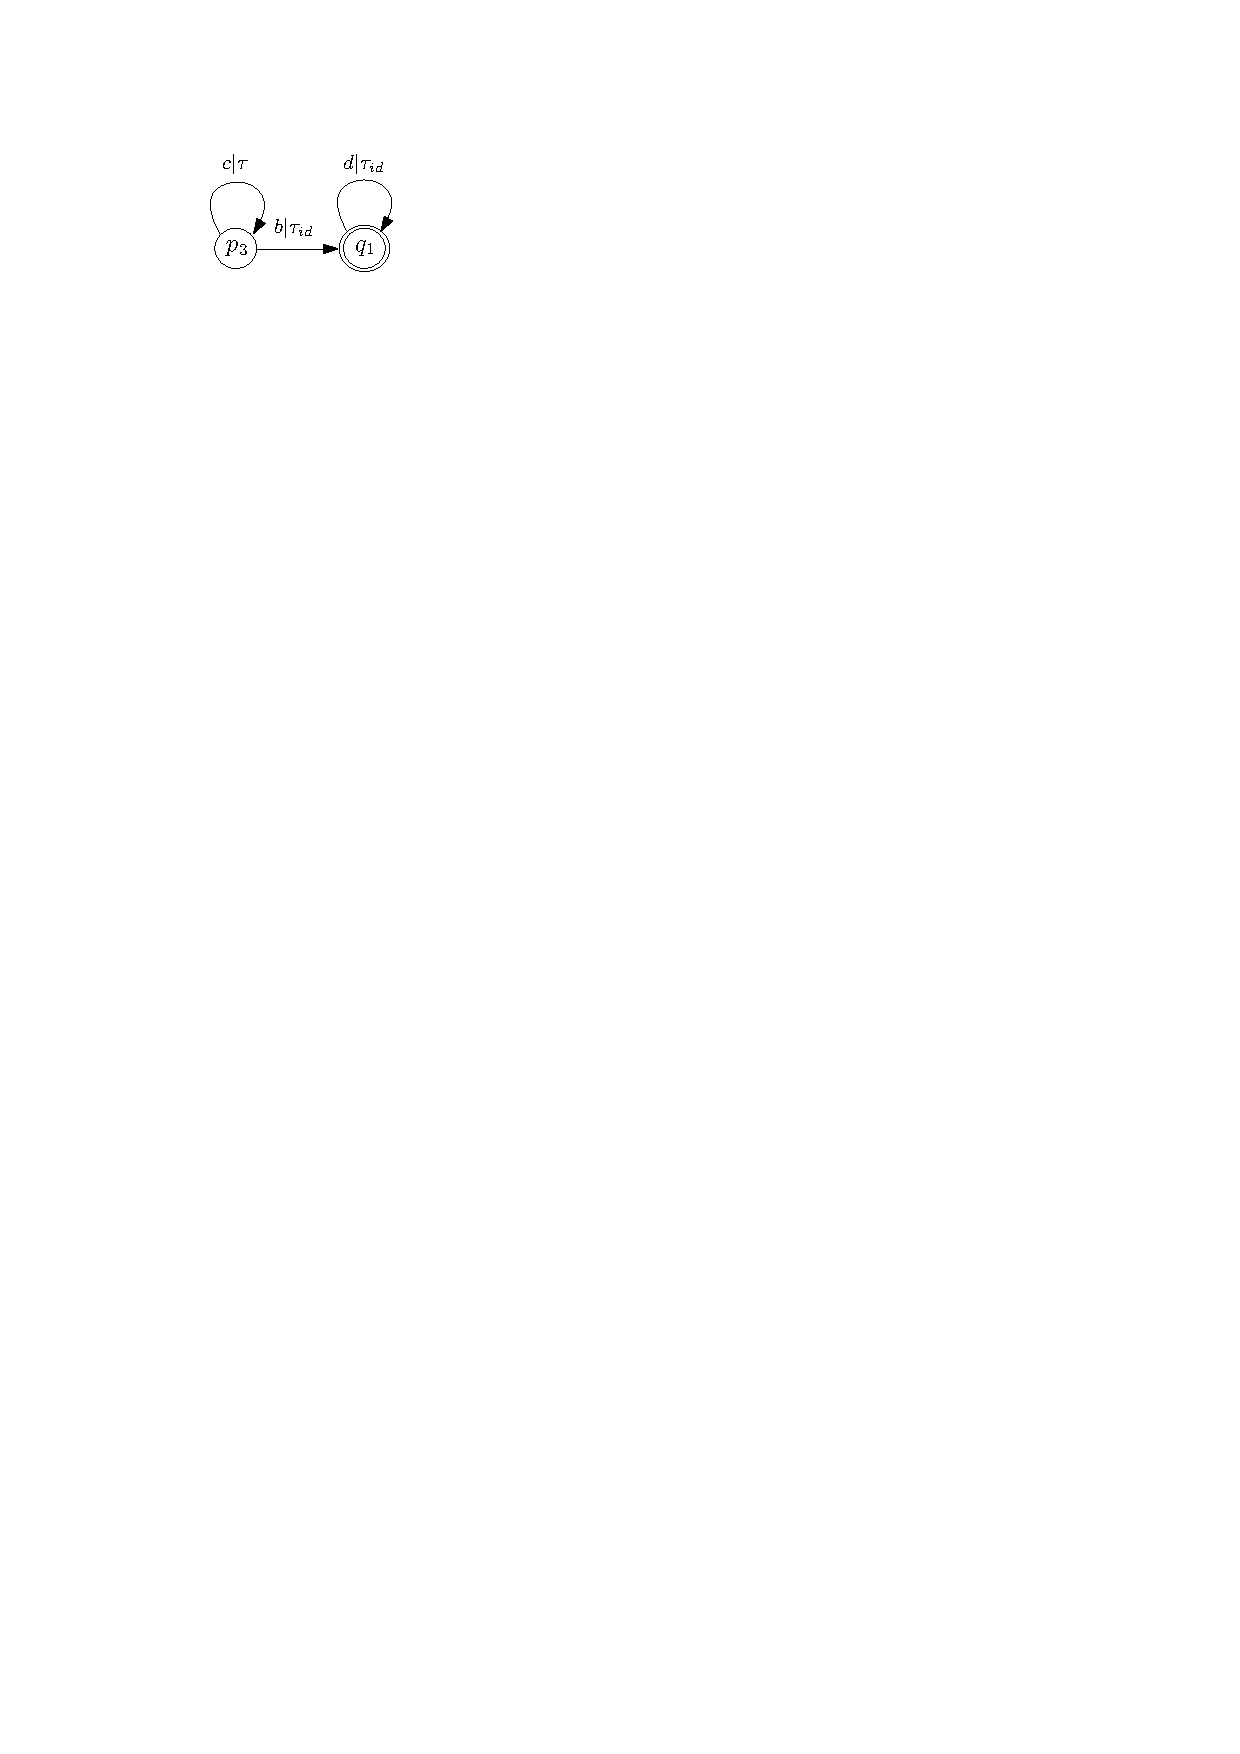
\includegraphics[scale = 0.9]{pwpotrnfa-example.pdf}
	\caption{An example of $\Pp$-\WOTrNFA}\label{fig-ptrnfa-exmp}
\end{figure}
\qed
\end{example}

For a $\Pp$-{\WOTrNFA} $\Aut$, $pre^*_\Pp(\ConfSet(\Aut))$  denotes the set of configurations $(p, w)$ of $\Pp$ such that $(p, w) \xRightarrow{\Pp} (p', w')$ for some $(p', w') \in \ConfSet(\Aut)$. Accordingly, $post^*_\Pp(\ConfSet(\Aut))$ denotes the set of configurations $(p, w)$ of $\Pp$ such that $(p', w') \xRightarrow{\Pp} (p, w)$ for some $(p', w') \in \ConfSet(\Aut)$.





%%%%%%%%%%%%%%%%%%%%%%%%%%%%%%%%%%%%%%%%%%%%%%%%%
%%%%%%%%%%%%%%%%%%%%%%%%%%%%%%%%%%%%%%%%%%%%%%%%%
\subsubsection{Saturation} \label{sect:decidability}
Let $\Pp = (P, \Gamma, \TranSet, \Delta)$ be a  {\WOTrPDS} where $\Tranbasis$, the union-basis of  $\langle \TranSet \rangle$, is a wpo, and let $\Aut = (Q, \Gamma, \delta, F)$ be a $\Pp$-{\NFA}. %We prove Theorem~\ref{thm-wstrpds-reach} by 
We apply the saturation procedures from \cite{SM+15,Song18} to obtain a $\Pp$-{\WOTrNFA} $\Aut^{\pre^*}$ (resp. $\Pp$-{\WOTrNFA} $\Aut^{\post^*}$), which represents $pre^*_\Pp(\ConfSet(\Aut))$ (resp. $post^*_\Pp(\ConfSet(\Aut))$).

% Let $\Pp = (P, \Gamma, \TranSet, \Delta)$ be a  {\WOTrPDS} where $\Tranbasis$, the union-basis of  $\langle \TranSet \rangle$, is a wpo, and let $\Aut = (Q, \Gamma, \delta, F)$ be a $\Pp$-{\NFA}. %We prove Theorem~\ref{thm-wstrpds-reach} by 
% We apply the saturation procedures from \cite{SM+15,Song18} to obtain a $\Pp$-{\WOTrNFA} $\Aut^{pre^*}$, which represents $pre^*_\Pp(\ConfSet(\Aut))$ and 
%represents the set of configurations reachable from the initial configuration. 
%The termination of the saturation procedures is guaranteed by the assumption that the transduction closure is well-ordered.  Then the regular reachability problem is reduced to the {\WOTrNFA}-{\NFA} intersection problem for $\Aut$ and $\AutB$, which is decidable according to Proposition~\ref{prop-wstrnfa-nfa-intersect}.
%
%In the sequel, we first recall the two saturation procedure in \cite{SM+15,Song18}, then prove its termination.
%
%Let $\Aut = (Q', \Gamma, \delta', P, F')$ be a $\Pp$-{\WOTrNFA} such that for each pair of states $(q_1, q_2)$ and each $\gamma \in \Gamma_\varepsilon$, there is at most one $\tau'' \in \langle \TranSet \rangle$ satisying that $(q_1, \gamma, \tau'', q_2) \in \delta'$. 
%
%The $\Pp$-{\WOTrNFA} $\Aut^{pre^*}$ 
\paragraph{Computing $pre^*$:}
$\Aut^{\pre^*}$ is constructed by iteratively adding the transitions to $\Aut$, according to the following saturation rule. 
%$\Aa^{pre^*} $ is obtained from $\Aa$ by adding the transitions according to the following three saturation rules.

\smallskip

\fbox{
%
\begin{minipage}{0.9\textwidth}
%\begin{enumerate}
    Let $\Aut'$ be the current $\Pp$-{\WOTrNFA}.
     For $(p_1, \gamma, w, \tau, p_2) \in \Delta$ and $p_2  \xRightarrow{w\mid\tau'} q'$ in $\Aut'$, suppose that a $\Tranbasis$-representation of $\tau\circ\tau'$ is $\beta_1 \cup \cdots \cup \beta_n$ where $\beta_i \in \Tranbasis$ for each $i \in [n]$,  %we do the following: 
%     Suppose that a $\Tranbasis$-representation of $\tau\circ\tau'$ is $\beta_1 \cup \cdots \cup \beta_n$ where $\beta_i \in \Tranbasis$ for each $i \in [n]$.
     %
     for each $i \in [n]$ such that there does \emph{not} exist a transition $(p_1, \gamma, \tau'', q')$ in $\Aut'$ with $\tau'' \preceq \beta_i$ (i.e. $\tau'' \supseteq \beta_i$),  we update $\Aut'$ by adding a transition $(p_1, \gamma, \beta_i, q')$.
     %
%     if there is a transition $(p_1, \gamma, \tau'', q')$ in the current $\Pp$-{\WOTrNFA}, then we replace $(p_1, \gamma, \tau'', q')$ with the transition $(p_1, \gamma, (\tau\circ\tau') \cup \tau'', q')$, otherwise, we add a transition $(p_1, \gamma,\tau\circ\tau', q')$.
%\end{enumerate}
\end{minipage}
}
\smallskip

\paragraph{Computing $post^*$:}
$\Aut^{\post^*}$ is constructed by iteratively adding the transitions to $\Aut$, according to the following saturation rule. 
%$\Aa^{pre^*} $ is obtained from $\Aa$ by adding the transitions according to the following three saturation rules.

\smallskip

\fbox{

\begin{minipage}{0.9\textwidth}
    Let $\Aut'$ be the current $\Pp$-{\WOTrNFA}. For $(p_1, \gamma, w, \tau, p_2) \in \Delta$, and $p_1  \xRightarrow{\gamma\mid\tau'} q'$ in $\Aut'$, 
    suppose that a $\Tranbasis$-representation of $\overline{\tau}\circ\tau'$ is $\beta_1 \cup \cdots \cup \beta_n$ where $\beta_i \in \Tranbasis$ for each $i \in [n]$, 
    \begin{enumerate}
        \item if $w = \epsilon$ or $w=\gamma_1$, for each $i \in [n]$ such that there does \emph{not} exist a transition $(p_2, w, \tau'', q')$ in $\Aut'$ with $\tau'' \preceq \beta_i$ (i.e. $\tau'' \supseteq \beta_i$),  we update $\Aut'$ by adding a transition $(p_2, w, \beta_i, q')$.
        \item if $w = \gamma_1\gamma_2$, 
            \begin{itemize}
                \item suppose that a $\Tranbasis$-representation of $\tau_{\id}$ is $\beta_1' \cup \cdots \cup \beta_m'$ where $\beta_i' \in \Tranbasis$ for each $i \in [m]$, then for each $i\in[m]$, we update $\Aut'$ by adding a transition $(p_2,\gamma_1,\beta_i',\langle p_2,\gamma_1\rangle)$,
                \item for each $i \in [n]$ such that there does \emph{not} exist a transition $(\langle p_2,\gamma_1\rangle, \gamma_2, \tau'', q')$ in $\Aut'$ with $\tau'' \preceq \beta_i$ (i.e. $\tau'' \supseteq \beta_i$), we update $\Aut'$ by adding a transition $(\langle p_2,\gamma_1\rangle, \gamma_2, \beta_i, q')$.
            \end{itemize}

    \end{enumerate}
\end{minipage}
}
\smallskip
%Note that the aforementioned saturation rule guarantees the following property is preserved in the construction: For each pair of states $(q_1, q_2)$ and each $\gamma \in \Gamma_\varepsilon$, there is at most one $\tau'' \in \langle \TranSet \rangle$ satisying that $(q_1, \gamma, \tau'', q_2) \in \delta'$.


We now show that the  saturation procedure for computing $\Aut^{pre^*}$ terminates. 
%The proof for computing $\Aut^{pre^*}$ is similar.
%
Towards contradiction, suppose that 
%the saturation procedure for computing $\Aut^{pre^*}$ 
it does not terminate. From the construction of $\Aut^{pre^*}$, there must be $q_1, q_2 \in Q'$, $\gamma \in \Gamma_\varepsilon$, and an infinite sequence of transductions $\beta_1, \beta_2, \cdots \in \Tranbasis$ such that the transitions $(q_1, \gamma, \beta_1, q_2) $, $(q_1, \gamma, \beta_2, q_2) $, $\cdots$ are added one by one,  and for every $i > 1$ and $j \le i$, $\beta_j \not \preceq \beta_i$,  that is, either $\beta_j$ and $\beta_i$ are incomparable or $\beta_j \succ \beta_i$. From infinite Ramsey theorem (cf. Theorem 9.1.2 in \cite{Rein00}), there must be an infinite sequence $i_1 < i_2 < \cdots$ such that $\beta_{i_1}, \beta_{i_2}, \cdots$ is either an infinite antichain or an infinite strictly descending chain. This contradicts the assumption that $(\Tranbasis, \preceq)$ is a wpo. 
%$\tau_1 \subset \tau_2 \subset \cdots$, that is, $\tau_1, \tau_2, \cdots$ is a strictly ascending chain with respect to $\subseteq$, thus a strictly descending chain with respect to $\preceq$. This contradicts the assumption that $(\langle \TranSet\rangle, \preceq) $ is a wpo.


\begin{example}
Let us continue Example~\ref{exmp-wpotrpds}. Let $\Aut = (Q, \Gamma, \delta, F)$ be the $\Pp$-{\NFA} recognizing the configurations $\{(p_3, b^m d^n \bot) \mid m > 0, n > 0\}$ (see Figure~\ref{fig-pnfa-exmp}). More specifically, $Q= P \cup \{q_1, q_2, q_3\}$, $F= \{q_3\}$, and $\delta$ is illustrated by the edges in Figure~\ref{fig-pnfa-exmp} (where the identity transduction $\tau_{id}$ in the transitions is omitted).  
%More specifically, $Q = \{p_3, q_1, q_2\}$
%
\begin{figure}[htb]
    \centering
	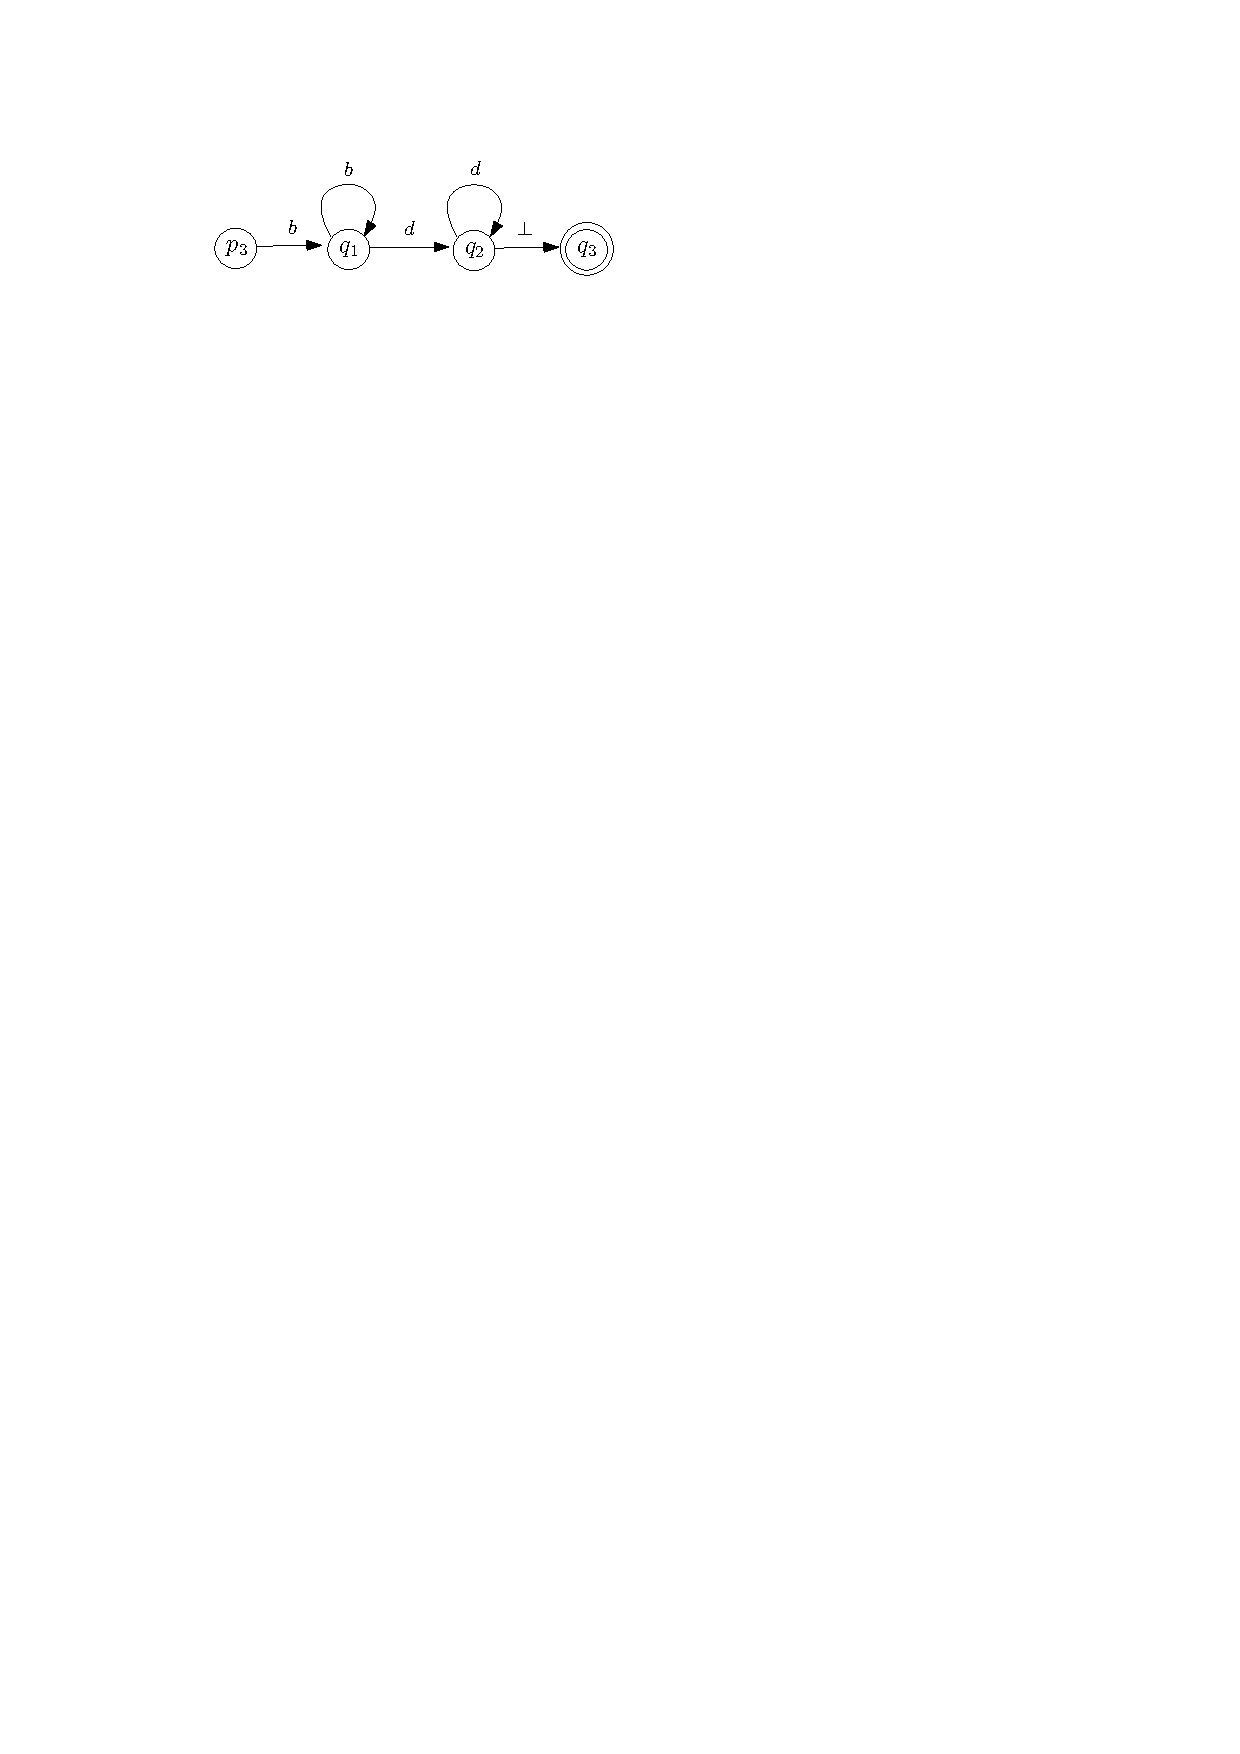
\includegraphics[scale = 0.9]{pnfa-example.pdf}
	\caption{An example of $\Pp$-{\NFA} $\Aut$}\label{fig-pnfa-exmp}
\end{figure}

Then we apply the saturation rule to add transitions.
\begin{itemize}
\item In the beginning, because $(p_3, a, \varepsilon, \tau_{id}, p_3) \in \Delta$ and $p_3 \xRightarrow{\varepsilon | \tau_{id}} p_3$ in $\Aut$, the transition $(p_3, a, \tau_{id}, p_3)$ is added according to the saturation rule. Similarly, the transition $(p_3, c, \tau_{id}, p_3)$ is added. 
%
\item Because $(p_3, c, ac, \tau, p_3) \in \Delta$, $p_3 \xRightarrow{ac | \tau_{id}} p_3$  in the current $\Pp$-{\WOTrNFA}, $\tau \circ \tau_{id} = \tau \in \Tranbasis$, and 
 there already exists a transition $(p_3, c, \tau_{id}, p_3)$, moreover, $\tau_{id} \not \preceq \tau$, the transition $(p_3, c, \tau, p_3)$ is added according to the saturation rule. 
%
\item Similarly, since $(p_2, b, cb, \tau_{id}, p_3) \in \Delta$, $p_3 \xRightarrow{cb | \tau_{id}} q_1$ and $p_3 \xRightarrow{cb | \tau} q_1$ in the current $\Pp$-{\WOTrNFA}, two transitions $(p_2, b, \tau_{id}, q_1)$  and $(p_2, b, \tau, q_1)$ are added. 
%
\item Furthermore, because $(p_1, a, ba, \tau_{id}, p_2) \in \Delta$ and $p_2 \xRightarrow{ba | \tau_{id} \cup \tau} q_2$ in the current $\Pp$-{\WOTrNFA} (This follows from $p_2 \xrightarrow{b | \tau} q_1$, $q_1 \xrightarrow{d | \tau_{id}} q_2$, and $(\lceil a, d\rfloor^{-1} \tau) \circ \tau_{id} = \tau_{id} \cup \tau$.), two transitions $(p_1, a, \tau_{id}, q_2)$  and $(p_1, a, \tau, q_2)$ are added.
%
%\item Furthermore, because $(p_2, b, cb, \tau_{id}, p_3) \in \Delta$, $p_3 \xRightarrow{cb | \tau} q_1$ in the current $\Pp$-{\WOTrNFA}, $ \tau_{id} \circ \tau = \tau \in \Tranbasis$, and there already exists a transition $(p_2, b, \tau_{id}, q_1)$, moreover, $\tau_{id} \not \preceq \tau$,
%the transition $(p_2, b, \tau, q_1)$ is added. 
\end{itemize}
By iterating this process, in the end, we obtain $\Aut^{pre*}$, as illustrated in Figure~\ref{fig-saturation-exmp}.
\begin{figure}[htb]
    \centering
	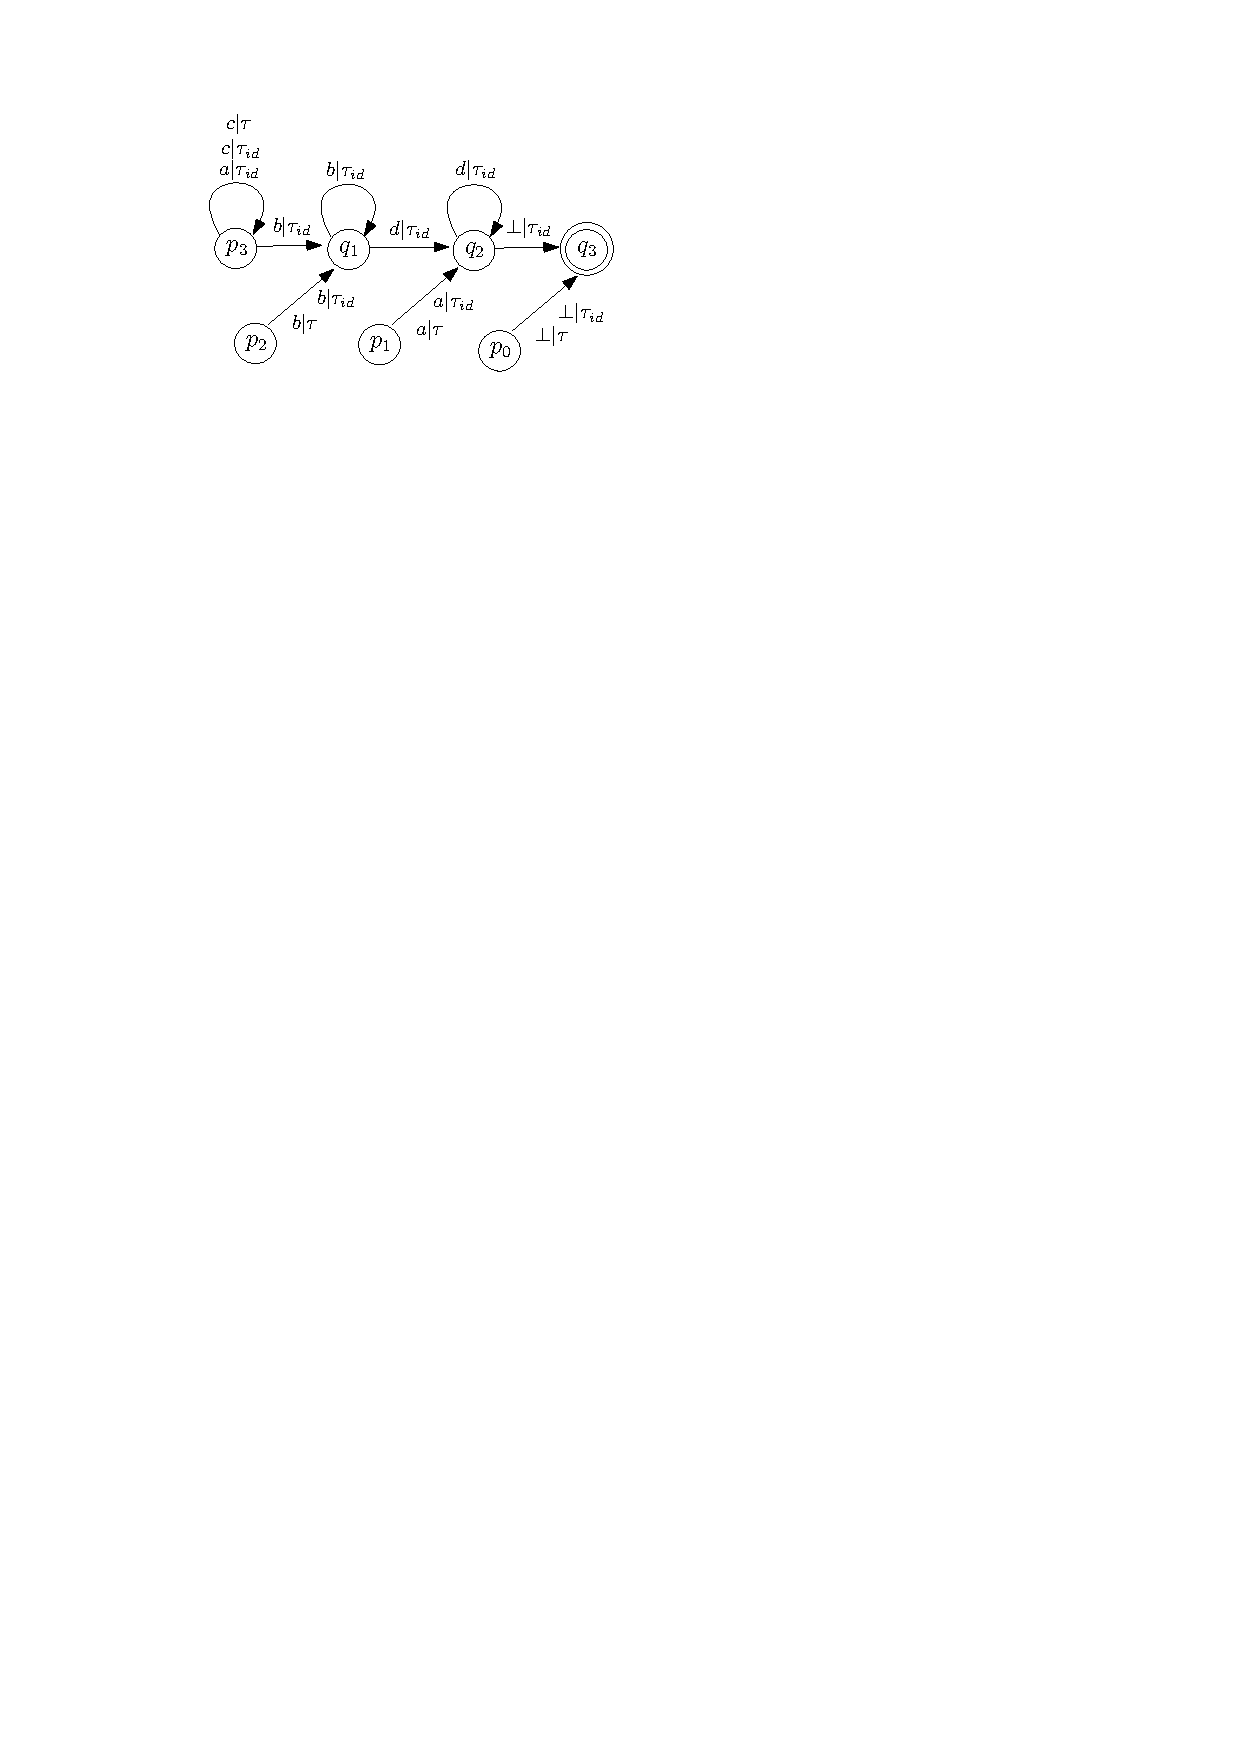
\includegraphics[scale = 0.9]{saturation-example.pdf}
	\caption{The $\Pp$-{\WOTrNFA} $\Aut^{pre*}$}\label{fig-saturation-exmp}
\end{figure}
\qed
\end{example}

Given the {\WOTrPDS} $\Pp= (P, \Gamma, \TranSet, \Delta)$, $p_1, p_2 \in P$, and two regular languages $L_1, L_2$ represented by {\NFA}s $\Aut_1 = (Q_1, \Gamma, \delta_1, I_1, F_1)$ and $\Aut_2 = (Q_2, \Gamma, \delta_2, I_2, F_2)$ respectively, the regular reachability problem is reduced to the intersection problem of the $\Pp$-{\WOTrNFA} $(\Aut_2[p_2])^{pre*}$ and the $\Pp$-{\NFA} $\Aut_1[p_1]$, 
i.e., checking $\ConfSet((\Aut_2[p_2])^{pre*}) \cap \ConfSet(\Aut_1[p_1]) \neq \emptyset$, where $\Aut_1[p_1]$ is obtained from $\Aut_1$ by adding a transition $(p_1, a, q)$ for each $(q_0, a, q) \in \delta_1$ with $q_0 \in I_1$, similarly for $\Aut_2[p_2]$. Then Theorem~\ref{thm-wstrpds-reach} follows from Proposition~\ref{prop-wstrnfa-nfa-intersect} in the next subsection.

%Here when we add a transition $(p,\gamma,\tau'',p')$ into $\Aa$, if there exists a transition $(p, \gamma,\tau',p')$ in the current automaton, we modify the transition $(p,\gamma,\tau',p')$ to $(p,\gamma,\tau'\cup\tau'',p')$ instead of adding $(p,\gamma,\tau'',p')$.


\subsubsection{The intersection problem of {\WOTrNFA} and {\NFA}} \label{sec:fatrnfa}
%\begin{definition}[{\WOTrNFA}-{\NFA} intersection problem]
The {\WOTrNFA}-{\NFA} intersection problem is, for given $\Pp$-{\WOTrNFA} $\Aut$ and $\Pp$-{\NFA} $\AutB$, to decide  whether $\ConfSet(\Aut) \cap \ConfSet(\AutB) = \emptyset$. We shall show that this problem %the {\WOTrNFA}-{\NFA} intersection problem to 
can be reduced to (polynomially many) instances of the sub-covering problem of a downward-WSTS, which is decidable by Theorem~\ref{thm-dwsts}.
%\end{definition}

%The rest of this section is devoted to the proof of the following result.
\begin{proposition}\label{prop-wstrnfa-nfa-intersect}
	The {\WOTrNFA}-{\NFA} intersection problem is decidable.
\end{proposition}

%For technical convenience, we define another partial order $\preceq$ on $\langle \TranSet \rangle$ as follows: $\tau_1 \preceq \tau_2$ if $\tau_1 \supseteq \tau_2$. Moreover, we use $\tau_1 \prec \tau_2$ to denote $\tau_1 \supset \tau_2$ (i.e. $\tau_1 \supseteq \tau_2$ but $\tau_1 \neq \tau_2$).

%From the fact that $(\langle \TranSet \rangle, \subseteq)$ is dually well-ordered, namely, it satisfies the ACC condition and contains no infinite antichain, we deduce that $(\langle \TranSet \rangle, \preceq)$ is well-ordered, namely, it satisfies the DCC condition and contains no infinite antichain.

%$(\langle \TranSet \rangle, \preceq)$ is well-ordered


%In the sequel, we are going to prove Proposition~\ref{prop-wstrnfa-nfa-intersect} by reducing 

%Its proof relies on the decidability of the sub-covering problem of downward-WSTS (\cite{FS01}).
% $(T, \rightarrow, \preceq)$.

\begin{proof}
%Let us fix a {\WOTrPDS} $\Pp = (P, \Gamma, \TranSet, \Delta)$, 
Assume a $\Pp$-{\WOTrNFA} $\Aut = (Q, \Gamma, \delta, F)$ and a $\Pp$-{\NFA} $\AutB = (Q', \Gamma, \delta', F')$.
We construct a downward-WSTS $\wstsnodes_{\Aut,\AutB} = (S, \rightarrow, \preceq)$ 
%
%The basic idea of $\wstsnodes_{\Aut,\AutB}$ is 
to simulate the synchronized runs of $\Aut$ and $\AutB$, where
\begin{itemize}
	\item $S = Q \times \Tranbasis \times Q'$, (Intuitively, $(q, \beta, q') \in S$ means that the current states of $\Aut$ and $\AutB$ are $q$ and $q'$ respectively, and $\beta$ is the transduction to be applied to the remaining suffix of the input string.)
	%
	\item the transition relation $\xrightarrow{}$ is defined as follows:  for every state $(q_1, \beta_1, q'_1)$ in $S$ and transition rules $(q_1, b, \beta, q_2) \in \delta$ and $(q'_1, a, q'_2) \in \delta'$, suppose that a $\Tranbasis$-representation of $( \lceil a, b \rfloor^{-1} \beta_1) \circ \beta$ is $\beta'_1 \cup \cdots \cup \beta'_k$,  then we have $(q_1, \beta_1, q'_1) \xrightarrow{} (q_2, \beta'_i, q'_2)$ for every $i \in [k]$, (Intuitively, $b$ is obtained from $a$ by applying the transduction $\beta_1$.)
%	
%	 and $(q_2, \tau_2, q'_2)$ in $ S$, $(q_1, \tau_1, q'_1) \rightarrow (q_2, \tau_2, q'_2)$ iff $\tau_1 \neq \emptyset$, and there are $a, b \in \Gamma_\varepsilon$ and a transduction $\tau$ such that $(q_1, b, \tau, q_2) \in \delta$, $(q'_1, a, q'_2) \in \delta'$, and $\tau_2 =( \lceil a, b \rfloor^{-1} \tau_1) \circ \tau$, 
	%
	\item for states $(q_1, \beta_1, q'_1)$ and $(q_2, \beta_2, q'_2)$ in $S$, $(q_1, \beta_1, q'_1) \preceq (q_2, \beta_2, q'_2)$ iff $q_1= q_2$, $q'_1 = q'_2$, and $\beta_1 \preceq \beta_2$.
\end{itemize}

To show that $\wstsnodes_{\Aut,\AutB} = (S, \rightarrow, \preceq)$ is a downward-WSTS, we first observe that $(S, \preceq)$ is a wpo since $(\Tranbasis, \preceq)$ is a wpo. Moreover, we shall show that $\rightarrow$ is downward reflexive-compatible with respect to $\preceq$. Namely, if $(q_1, \beta_1, q'_1) \rightarrow (q_2, \beta_2, q'_2)$ and $(q_1, \beta_1, q'_1) \succeq (q_3, \beta_3, q'_3)$, then there is $(q_4, \beta_4, q'_4)$ such that $(q_3, \beta_3, q'_3) \rightarrow (q_4, \beta_4, q'_4)$ and $(q_2, \beta_2, q'_2) \succeq (q_4, \beta_4, q'_4)$. 

From $(q_1, \beta_1, q'_1) \rightarrow (q_2, \beta_2, q'_2)$, there are $a, b \in \Gamma_\varepsilon$ and $\beta \in \Tranbasis$ such that $(q_1, b, \beta, q_2) \in \delta$, $(q'_1, a, q'_2) \in \delta'$, and $\beta_2$ occurs as a disjunct in a $\Tranbasis$-representation of $( \lceil a, b \rfloor^{-1} \beta_1) \circ \beta$. 

From $(q_1, \beta_1, q'_1) \succeq (q_3, \beta_3, q'_3)$, we have that $q_1 = q_3$, $q'_1 = q'_3$, and $\beta_3 \preceq \beta_1$. Therefore, $ ( \lceil a, b \rfloor^{-1} \beta_3) \circ \beta \preceq ( \lceil a, b \rfloor^{-1} \beta_1) \circ \beta$. Furthermore, since $\beta_2 \subseteq ( \lceil a, b \rfloor^{-1} \beta_1) \circ \beta $, we have $( \lceil a, b \rfloor^{-1} \beta_1) \circ \beta  \preceq \beta_2$. Then $ ( \lceil a, b \rfloor^{-1} \beta_3)  \circ \beta \preceq \beta_2$. From the distributivity of $\preceq$ over $\Tranbasis$-representations, we know that there is a disjunct $\beta_4$ of a $\Tranbasis$-representation of $( \lceil a, b \rfloor^{-1} \beta_3)  \circ \beta$ such that $\beta_4 \preceq \beta_2$.
Let $q_4 = q_2$ and $q'_4= q'_2$. Then $(q_1, \beta_3, q'_1) \rightarrow (q_2, \beta_4, q'_2)=(q_4, \beta_4, q'_4)$ and $(q_2, \beta_2, q'_2) \succeq (q_4, \beta_4, q'_4)$.

%From $(q_1, \beta_1, q'_1) \succeq (q_3, \beta_3, q'_3)$, we know that $q_1 = q_3$, $q'_1 = q'_3$, and $\beta_1 \subseteq \beta_3$.  Therefore, $\beta_2 = ( \lceil a, b \rfloor^{-1} \beta_1) \circ \tau \subseteq ( \lceil a, b \rfloor^{-1} \beta_3) \circ \tau = \beta_4$. We deduce that $\tau_2 \succeq \tau_4$ and $(q_2, \tau_2, q'_2) \succeq (q_4, \tau_4, q'_4)$. 

Therefore, $\rightarrow$ is downward reflexive-compatible with respect to $\preceq$. Furthermore, we show that $\wstsnodes_{\Aut,\AutB}$ has effective $\Succ$ and decidable $\preceq$.
\begin{itemize}
	%\item Since $(\wstsnodes_{\Aut,\AutB}, \rightarrow, \preceq)$ has strong downward-compatibility, it follows that it also has reflexive downward-compatibility.
	%
	\item Given a state $(q_1, \beta_1, q'_1)$, $\Succ((q_1, \beta_1, q'_1))$ can be computed effectively as follows: Enumerate all the pairs of transition rules $(q_1, b, \beta, q_2) \in \delta$ (there are only finitely many of them) and $(q'_1, a, q'_2) \in \delta'$, and for every such pair of transitions, compute a $\Tranbasis$-representation of $( \lceil a, b \rfloor^{-1} \beta_1) \circ \beta$, say $\beta'_1 \cup \cdots \cup \beta'_k$, then for each $i \in [k]$, put $(q_2, \beta'_i, q'_2)$ into $\Succ((q_1, \beta_1, q'_1))$.
	%
	\item Finally, given two states $(q_1, \tau_1, q'_1)$ and $(q_2, \tau_2, q'_2)$ (where $\tau_1, \tau_2$ are given as {\NFT}s), from Proposition~\ref{prop-nft-inclusion}, we can effectively decide whether $\tau_1 \preceq \tau_2$, namely, $\tau_2 \subseteq \tau_1$. Therefore, $\wstsnodes_{\Aut,\AutB}$ has decidable $\preceq$.
\end{itemize}

Then $\ConfSet(\Aut) \cap \ConfSet(\AutB) \neq \emptyset$ iff $p \xRightarrow{w | \tau} q$, $p \xRightarrow{w} q'$, and $(\varepsilon, \varepsilon) \in \tau$ for some $p \in P$, $w \in \Gamma^*$, $\tau \in \langle \TranSet \rangle$, $q \in F$, and $q' \in F'$. Suppose that a $\Tranbasis$-representation of $\tau_{id}$ is $\beta_1 \cup \cdots \cup \beta_k$. 
The construction of $\wstsnodes_{\Aut,\AutB}$ entails that $p \xRightarrow{w | \tau} q$, $p \xRightarrow{w} q'$, and $(\varepsilon, \varepsilon) \in \tau$ for some $w \in \Gamma^*$  and $\tau \in \langle \TranSet \rangle$  iff $(q, \beta', q')$ is reachable from $(p, \beta_i, p)$ in $\wstsnodes_{\Aut,\AutB}$ and $\beta' \preceq \tau_\varepsilon$ for some $\beta' \in \Tranbasis$ and $i \in [k]$, where $\beta'$ occurs as a disjunct of a $\Tranbasis$-representation of $\tau$. 
%
Furthermore, $(q, \beta', q')$ is reachable from $(p, \beta_i, p)$ in $\wstsnodes_{\Aut,\AutB}$ and $\beta' \preceq \tau_\varepsilon$ for some $\beta' \in \Tranbasis$ and $i \in [k]$ iff $(q, \beta', q')$ is reachable from $(p, \beta_i, p)$ in $\wstsnodes_{\Aut,\AutB}$ and $(q, \beta', q')$ sub-covers $(q, \tau_\varepsilon, q')$ for some $\beta' \in \Tranbasis$ and $i \in [k]$. Therefore, we deduce that \emph{$\ConfSet(\Aut) \cap \ConfSet(\AutB) \neq \emptyset$ iff there are $p \in P$, $q \in F$, $q' \in F'$, and $i \in [k]$ such that starting from $(p, \beta_i, p)$, a state that sub-covers $(q, \tau_\varepsilon, q')$ can be reached}.
%\end{quote}
We conclude from Theorem~\ref{thm-dwsts} that the {\WOTrNFA}-{\NFA} intersection problem is decidable.
\end{proof}


\subsubsection{Proof of Theorem~\ref{thm:st-amass-reach}}\label{sec-proof-reach}
Our idea is to ues {\WOTrPDS} $\Pp_{\Mm}$ to simulate the behaviors fo $\Mm$, recall that we use $\tau_{B, A}$ to simulate $A\xrightarrow{\startactivity(\phi_{\rtfflag})}B$ with $\phi_{\rtfflag}\models\rtfflag\wedge\neg\ctpflag$.
However, such a direct simulation would entail an \emph{infinite} antichain in the transduction closure: $\tau^n_{B, A}$  (where $n \ge 1$), i.e. the $n$-fold composition of $\tau_{B,A}$, is the transduction that removes the first $n$ occurrences of $B$ from the input string and add $n$ $A$'s in the beginning. It is easy to observe that for every $i, j$ with $i \neq j$, $\tau^i_{B, A}$ and $\tau^j_{B, A}$ are incomparable with respect to $\preceq$, namely, neither $\tau^i_{B, A} \subseteq \tau^j_{B, A}$, nor $\tau^j_{B, A} \subseteq \tau^i_{B, A}$. Therefore, $\tau_{B, A}, \tau^2_{B, A}, \tau^3_{B, A}, \cdots$ comprises an infinite antichain with respect to $\preceq$. 

To ensure that the transduction closure of $\Pp_\Mm$  has a well-partially-ordered union-basis, we
apply the following tricks: when simulating $A\xrightarrow{\startactivity(\phi_{\rtfflag})}B$ with $A \neq B$,
\begin{itemize}
\item instead of moving the first occurrence of $B$ to the beginning of the input string, we replace the first occurrence of $B$ with a dummy symbol $\dag$ and push $B$ into the stack, and
%
\item $A\xrightarrow{\startactivity(\phi_{\rtfflag})}B$ is simulated by the transition rules $p \xrightarrow{A / BA | \tau_{B, \dag}} p$ and  $p \xrightarrow{A / BA | \tau_{\not B}} p$, where $\tau_{B, \dag}$ is the transduction that replaces \emph{at least the first occurrence of $B$ with $\dag$}. More precisely, $\tau_{B, \dag}$ nondeterministically chooses some $n \ge 1$ and replaces each of the first $n$ occurrences of $B$ with $\dag$.
\end{itemize}
%\tl{revisit here}
The aforementioned tricks are justified by the observation that the transition $A\xrightarrow{\startactivity(\phi_{\rtfflag})}B$ could be continuously applied for multiple times: Namely, when the topmost occurrence of $B$ is moved to the top of the stack, $B$ can be popped and $A$ becomes the top activity of the stack again. Then the transition $A\xrightarrow{\startactivity(\phi_{\rtfflag})}B$ can be applied for the second time to move the top second occurrence of $B$  (referring to the original contents of the stack) to the top. Furthermore, this process can be continued if there are still some occurrences of $B$ in the stack. Therefore, the simulation of $A\xrightarrow{\startactivity(\phi_{\rtfflag})}B)$ by $p \xrightarrow{A / BA | \tau_{B, \dag}} p$ and  $p \xrightarrow{A / BA | \tau_{\not B}} p$ is sound in the sense that it does \emph{not} introduce unreachable configurations.

%We first show that a  {\ASS} $\Aut = (Act, A_0,\Delta)$ can be simulated by a pushdown system with transductions $\Pp_\Aut = (P_\Aut, \Gamma_\Aut, \TranSet_\Aut, \Delta_\Aut)$. Then we prove that $(\langle \TranSet_\Aut \rangle, \preceq)$ is well-ordered, that is, $\Pp_\Aut$ is a {\WOTrPDS}. The decidability of the configuration reachability problem of {\ASS} then follows from Theorem~\ref{thm-wstrpds-reach}.

\paragraph*{From $\Mm$ to $\Pp_\Mm$} 
The {\WOTrPDS} $\Pp_\Mm = (P_\Mm, \Gamma_\Mm, \TranSet_\Mm, \Delta_\Mm)$ where 
\begin{itemize}
\item $P_{\Mm} = \{p_0\}\cup\{ p_{B}\mid B\in\act\}$,
\item $\Gamma_{\Mm} = \act \cup \{\dag\}$, 
\item $\TranSet_\Mm = \{\tau_{\id} \}\cup \{\tau_{B, \dag} \mid B \in \act\} \cup \{\tau_{B} \mid B \in \act\}  \cup \{\tau_{\not B} \mid B \in \act\}$, where $\tau_B$ is the transduction that checks that $B$ occurs in the input string but keeps the input string unchanged, and 
\item $\Delta_{\Mm}$ is defined as follows:
        \begin{itemize}
            \item for each $A \in \act$, $(p_0, A, \varepsilon, \tau_{\id}, p_0) \in \Delta_{\Mm}$, (Recall that $\POP$ can be applied anytime in $\Mm$.)
			\item for each transition $A\xrightarrow{\startactivity(\phi)}B$, 
			\begin{itemize}
				\item if $\phi\models\stpflag$ and $A\neq B$, or $\phi=\bot$, we have $(p_0, A, BA, \tau_{\id}, p_0) \in \Delta_{\Mm}$, 
				\item if $\phi\models\ctpflag$, such that $A\neq B$, we have 
				\begin{itemize}
					\item $(p_0, A, BA, \tau_{\not B}, p_0) \in \Delta_{\Mm}$, 
					\item $(p_0, A, \varepsilon, \tau_{B}, p_B) \in \Delta_{\Mm}$, $(p_B, B, B, \tau_{\id}, p_0)  \in \Delta_{\Mm}$, and for each $\gamma \in \Gamma_\Mm \setminus \{B\}$, $(p_B, \gamma, \varepsilon, \tau_{\id}, p_B) \in \Delta_{\Mm}$, 
				\end{itemize}
				\item if $\phi\models\rtfflag\wedge\neg\ctpflag$, such that $A\neq B$, we have 
                we have $(p_0, A, BA, \tau_{\not B}, p_0) \in \Delta_{\Mm}$ 
                and $(p_0, A, BA, \tau_{B, \dag}, p_0) \in \Delta_{\Mm}$.
			\end{itemize}
            %
        \end{itemize}
\end{itemize}
%$\tau_{\CTK} = (\{p_0, q_f\}, \Gamma \cup \{\dag, \bot\}, \delta_{\CTK}, p_0, \{q_f\})$, where $\delta_{\CTK}$ is defined as follows.
%\begin{itemize}
%    \item for each $\gamma \in \Gamma \cup \{\dag\}$, we have $(p_0, \gamma, \dag, p_0) \in \delta_{\CTK}$,
%    \item we have $(p_0, \bot, \bot, q_f) \in \delta_{\CTK}$.
%\end{itemize}
%Intuitively, $\tau_{\CTK}$ transduces $w\bot$ into $\dag^{|w|}\bot$.



To show that $\Pp_\Mm$ is a {\WOTrPDS}, it is sufficient to show the following result. 
%$\langle \TranSet_\Aut \rangle$ has a union-basis $\Tranbasis$ satisfying the four conditions in Definition~\ref{def:defatpds}.

\begin{proposition}\label{lem-transet-wo}
$\langle \TranSet_\Mm \rangle$ has a union-basis $\Tranbasis$ satisfying the four conditions in Definition~\ref{def:defatpds}.
\end{proposition}

We now complete the proof of Theorem~\ref{thm:st-amass-reach}. For a given {\NFA} $\AutB = (Q, \act, \delta, I, F)$ over $\act$, let $\AutB'$ be the {\NFA} obtained from $\AutB$ by adding the transitions $(q, \dag, q)$ for every $q \in Q$. Then $\ConfSet(\Mm) \cap \ConfSet(\AutB) \neq \emptyset$ iff there is $w \in \ConfSet(\AutB')$ such that $(p_0, A_0) \xRightarrow{\Pp_\Mm} (p_0, w)$.
%$pre^*_{\Pp_\Aut}(\ConfSet(\AutB'[p_0])) \cap \{(p_0, A_0)\} \neq \emptyset$, where $\AutB'[p_0]$ is obtained from $\AutB'$ by adding the state $p_0$ and the transitions $(p_0, a, q)$ for all $(p, a, q) \in \delta$ with $p \in I$. 
From Theorem~\ref{thm-wstrpds-reach}, we conclude that Theorem~\ref{thm:st-amass-reach} holds.

The rest of this section is devoted to the proof of Proposition~\ref{lem-transet-wo}, Proposition~\ref{prop-tranbasis-ef} and Proposition~\ref{prop-tranbasis-udist}.


\subsection*{Proof of Proposition~\ref{lem-transet-wo}}
To prove Proposition~\ref{lem-transet-wo}, we first define $\Tranbasis_\Mm$.
For technical convenience, we fix a linear order $<$ on $Act$. Moreover, we introduce some additional notations for transductions.
\begin{itemize}
\item $\tau_\dag$ (resp. $\tau_{\not \dag}$) is the transduction that checks that $\dag$ occurs at least once (resp. $\dag$ does not occur), but keep the input string unchanged, 
%
\item $\tau_{\mathcircled{\Lambda}}$ is the transduction that checks that the set of symbols occurring in the input string is exactly $\Lambda$, %(i.e. all the symbols in the input string are from $\Lambda$ and each symbol in $\Lambda$ occurs in the input string), 
but keeps the input string unchanged. 
\end{itemize}

We then define $\Tranbasis_\Mm$ as the union of $\{\emptyset, \tau_\varepsilon\}$ and the set of transductions of the  form $\tau_{\dag} \circ \tau^{n_1}_{A_1, \dag} \circ \cdots \circ \tau^{n_k}_{A_k, \dag} \circ \tau_{\mathcircled{\Lambda}}$ or $\tau_{\not \dag} \circ \tau^{n_1}_{A_1, \dag} \circ \cdots \circ \tau^{n_k}_{A_k, \dag} \circ \tau_{\mathcircled{\Lambda}}$ such that 
1) $A_i \in Act$ and $n_i \ge 1$ for every $i \in [k]$, 
2) $A_1 < \cdots < A_k$ (which implies that they are distinct), 
3) $\Lambda \subseteq \Gamma_\Mm$ is nonempty. Note that here it is possible that $k=0$.

It remains to show that $\Tranbasis_\Aut$ satisfies the four conditions in Definition~\ref{def:defatpds}.

First, by the definition of $\Tranbasis_\Aut$, we have that $\{\emptyset, \tau_{\varepsilon}\} \subseteq \Tranbasis_\Aut$.

To show that $(\Tranbasis_\Aut, \preceq)$ is a wpo, it is sufficient to show that for every $k > 0$, $A_1 < \cdots < A_k$, and $\emptyset \neq \Lambda \subseteq \Gamma_\Aut$, the set of transductions of the form $\tau_{\alpha} \circ \tau^{n_1}_{A_1, \dag} \circ \cdots \circ \tau^{n_k}_{A_k, \dag} \circ \tau_{\mathcircled{\Lambda}}$  is a wpo (where $\alpha \in \{\dag, \not \dag\}$).  
%
It is easy to observe that if $\tau_{\alpha} \circ \tau^{n_1}_{A_1, \dag} \circ \cdots \circ \tau^{n_k}_{A_k, \dag} \circ \tau_{\mathcircled{\Lambda}} \neq \emptyset$ and $\tau_{\alpha} \circ \tau^{n'_1}_{A_1, \dag} \circ \cdots \circ \tau^{n'_k}_{A_k, \dag} \circ \tau_{\mathcircled{\Lambda}} \neq \emptyset$, 
then 
$\tau_{\alpha} \circ \tau^{n_1}_{A_1, \dag} \circ \cdots \circ \tau^{n_k}_{A_k, \dag} \circ \tau_{\mathcircled{\Lambda}} \preceq \tau_{\alpha} \circ \tau^{n'_1}_{A_1, \dag} \circ \cdots \circ \tau^{n'_k}_{A_k, \dag} \circ \tau_{\mathcircled{\Lambda}}$ iff $\tau_{\alpha} \circ \tau^{n_1}_{A_1, \dag} \circ \cdots \circ \tau^{n_k}_{A_k, \dag} \circ \tau_{\mathcircled{\Lambda}} \supseteq \tau_{\alpha} \circ \tau^{n'_1}_{A_1, \dag} \circ \cdots \circ \tau^{n'_k}_{A_k, \dag} \circ \tau_{\mathcircled{\Lambda}}$ iff $n_1 \le n'_1$, $\cdots$, and $n_k \le n'_k$. According to Dickson's lemma \cite{Kruskal72,Milner1985},  $(\Nat^k, \leq)$ is a wpo. We deduce that  $(\Tranbasis_\Aut, \preceq)$ is a wpo.

The verification of the third and fourth conditions in Definition~\ref{def:defatpds} for $\Tranbasis_\Aut$ is given by the following two propositions.

\begin{proposition}\label{prop-tranbasis-ef}
For each $\tau \in \langle \TranSet_\Mm \rangle$, a $\Tranbasis_\Mm$-representation $\beta_\tau$ can be computed effectively.
\end{proposition}

\begin{proposition}\label{prop-tranbasis-udist}
$\preceq$ is union-distributive over $\Tranbasis_\Mm$-representations.
\end{proposition}


\subsection*{Proof of Proposition~\ref{prop-tranbasis-ef}}
\begin{proof}
	We prove by a structural induction on the definition of $\langle \TranSet_\Mm \rangle$.
	
%	We first notice that every finite union of {\UFNF} $\beta_1 \cup \cdots \cup \beta_m$ can be turned into an {\AUNF} $\beta'_1 \cup \cdots \cup \beta'_n$, where $\beta'_1, \cdots, \beta'_n$ are antichains, by iterating the following process until no more {\UFNF} can be removed: if $\beta_i \preceq \beta_j$ (that is, $\beta_j \subseteq \beta_i$),  we remove $\beta_j$. Therefore, in the proof below, to show   $\beta_1 \cup \cdots \cup \beta_m$ is an {\AUNF}, we only need to show (i) in Definition~\ref{def-nf}.
	%ignore the requirement that $\beta_1, \cdots, \beta_m$ are antichains.
	
	\smallskip
	\noindent \emph{Base case.} We show that $\tau_{id}$ and all $\tau_{B}$, $\tau_{\not B}$, and $\tau_{B, \dag}$ for $B \in Act$ can be rewritten as $\Tranbasis_\Mm$-representations.
	%
	\begin{itemize}
	\item $\tau_{id} = \bigcup\limits_{\emptyset \neq \Lambda  \subseteq\Gamma_{\Mm}} (\tau_\dag \circ \tau_{\Lambda} \cup \tau_{{\not \dag}} \circ \tau_{\Lambda})$, 
	%
	\item $ \tau_{B} = \bigcup\limits_{ \Lambda \subseteq\Gamma_{\Mm}, B \in \Lambda} (\tau_\dag \circ \tau_{\Lambda} \cup \tau_{{\not \dag}} \circ \tau_{\Lambda}),$
	% \cup \left(\bigcup\limits_{\Lambda \subseteq \Gamma_{\Aut}\setminus \{\dag\}, B \in \Lambda} \tau_{\not \dag} \circ \tau_{\Lambda}\right),$$  
	%
	\item	$ \tau_{\not B} =
	\bigcup\limits_{\emptyset \neq \Lambda \subseteq\Gamma_{\Mm}, B \not \in \Lambda} (\tau_\dag \circ \tau_{\Lambda} \cup \tau_{\not \dag} \circ \tau_{\Lambda}),$  
	%
	\item $\tau_{B,\dag} = \bigcup\limits_{\emptyset \neq \Lambda \subseteq \Gamma_{\Mm}}(\tau_{\dag} \circ \tau_{B,\dag}^1\circ\tau_{\Lambda} \cup \tau_{\not \dag} \circ \tau_{B,\dag}^1\circ\tau_{\Lambda} )$.
	%
%	$\emptyset =\tau_\dag \circ \tau_{\{A\}}$ for every $A \in Act$. 
	%Note that the composition of $\tau_{A,\dag}^1$ and  $\tau_{\{A\}}$ is equal to $\emptyset$, since $\tau_{A,\dag}^1$ implies that $\dag$ must occur in the output string of $\tau_{A,\dag}^1$, while $\tau_{\{A\}}$ requires that $\dag$ does not occur.
	%
%	\item $\tau_{\id} = \bigcup\limits_{\emptyset \neq \Lambda \subseteq \Gamma_{\Aut}}(\tau_\dag \circ \tau_{\Lambda} \cup \tau_{\not \dag} \circ \tau_\Lambda)$.
	\end{itemize}
	
	For the induction step, we show the following claim. 
	
	\noindent \emph{Claim. Suppose that $\beta_1, \beta_2 \in \Tranbasis_\Mm$ and $\gamma, \gamma' \in \Gamma_\Mm$. Then $\beta_1 \circ \beta_2$ and $\lceil \gamma, \gamma' \rfloor^{-1}\beta_1$ can be rewritten into $\Tranbasis_\Mm$-representations.}
	
	\smallskip
	
	\noindent \emph{Proof of the claim.}
	%
	We consider $\beta_1 \circ \beta_2$ first.
	%

	Suppose that $\beta_1 = \tau_{\alpha_1} \circ \tau^{n_{1,1}}_{A_{1,1}, \dag} \circ \cdots \circ \tau^{n_{1, k_1}}_{A_{1,k_1}, \dag} \circ \tau_{\mathcircled{\Lambda_1}}$ and $\beta_2 = \tau_{\alpha_2} \circ \tau^{n_{2,1}}_{A_{2,1}, \dag} \circ \cdots \circ \tau^{n_{2, k_2}}_{A_{2,k_2}, \dag} \circ \tau_{\mathcircled{\Lambda_2}}$, where $\alpha_1, \alpha_2 \in \{\dag, \not \dag\}$.
	
	If $\beta_1 \circ \beta_2 = \emptyset$, then $\emptyset$ is already a $\Tranbasis_\Mm$-representation of $\beta_1 \circ \beta_2$. 
	
	Below we assume that $\beta_1 \circ \beta_2 \neq \emptyset$. This implies that $\beta_1 \neq \emptyset$ and $\beta_2 \neq \emptyset$.
	% 
	We exemplify the proof for the case that $\alpha_1 = {\not \dag}$ and  $\alpha_2 = \dag$.
	
	In this case, $\Lambda_1 =  \{A_{2,1}, \cdots, A_{2, k_2}\} \cup \Lambda_2$. The arguments proceed as follows. 
	Each symbol in the outputs of $\beta_1$ must be either in $\{A_{2,1}, \cdots, A_{2, k_2}\}$ or in $\Lambda_2$, i.e., $\Lambda_1 \subseteq   \{A_{2,1}, \cdots, A_{2, k_2}\} \cup \Lambda_2$. On the other hand, all the symbols in $\{A_{2,1}, \cdots, A_{2, k_2}\} \cup \Lambda_2$, except $\dag$, must occur in the inputs of $\beta_2$, namely, the outputs of $\beta_1$, thus  $(\{A_{2,1}, \cdots, A_{2, k_2}\} \cup \Lambda_2) \setminus \{\dag\} \subseteq \Lambda_1$.
	Therefore, we have that
	$(\{A_{2,1}, \cdots, A_{2, k_2}\} \cup \Lambda_2) \setminus \{\dag\} \subseteq \Lambda_1 \subseteq  \{A_{2,1}, \cdots, A_{2, k_2}\} \cup \Lambda_2$, that is, $\Lambda_1 = (\{A_{2,1}, \cdots, A_{2, k_2}\} \cup \Lambda_2) \setminus \{\dag\}$ or $\Lambda_1 =  \{A_{2,1}, \cdots, A_{2, k_2}\} \cup \Lambda_2$.
	%
	Moreover, $\alpha_2 = \dag$, and thus $\dag \in \Lambda_1$. Hence  $\Lambda_1 =  \{A_{2,1}, \cdots, A_{2, k_2}\} \cup \Lambda_2$.
	%
	%If $\Lambda_1 = (\{A_{2,1}, \cdots, A_{2, k_2}\} \cup \Lambda_2) \setminus \{\dag\}$, then $k_1 = 0$ (otherwise, $\dag \in \Lambda_1$). 
	%
	%Since $\beta_2 \neq \emptyset$ implies that all the symbols in $\{A_{2,1}, \cdots, A_{2, k_2}\} \cup \Lambda_2$, except $\dag$, must occur in the input strings of $\beta_2$,  we deduce that 
	%$$\beta_1 \circ \beta_2 = \tau_{\not \dag} \circ \tau_{\Lambda_1} \circ \beta_2 = 
	%\tau_{\not \dag} \circ \tau^{n_{2,1}}_{A_{2,1}, \dag} \circ \cdots \circ \tau^{n_{2, k_2}}_{A_{2,k_2}, \dag} \circ \tau_{\mathcircled{\Lambda_2}}.$$
	%
	
	Furthermore, we have $k_1 > 0$ because otherwise $\beta_1 = \tau_{\not \dag} \circ \tau_{\Lambda_1} = \emptyset$, contradicting the assumption that $\beta_1 \circ \beta_2 \neq \emptyset$. 
	%
	%$\beta_1 \circ \beta_2 = \tau_{\not \dag} \circ \tau_{\Lambda_1} \circ \beta_2 = 
	%\tau_{\dag} \circ \tau^{n_{2,1}}_{A_{2,1}, \dag} \circ \cdots \circ \tau^{n_{2, k_2}}_{A_{2,k_2}, \dag} \circ \tau_{\mathcircled{\Lambda_2}}$.
	%
	%Since $k_1 > 0$, we do not know for sure that $\dag$ occurs in the input strings of $\beta_1$. Therefore, 
	Consequently, 
	%
	$$\beta_1 \circ \beta_2 = 
	%\tau_{\dag} \circ \tau^{n'_{1}}_{A'_{1}, \dag} \circ \cdots \circ \tau^{n'_{k'}}_{A'_{k'}, \dag} \circ \tau_{\mathcircled{\Lambda_2}}\ \cup\ 
	\tau_{\not \dag} \circ \tau^{n'_{1}}_{A'_{1}, \dag} \circ \cdots \circ \tau^{n'_{k'}}_{A'_{k'}, \dag} \circ \tau_{\mathcircled{\Lambda_2}},$$
	%
	%
	where $\tau^{n'_{1}}_{A'_{1}, \dag} \circ \cdots \circ \tau^{n'_{k'}}_{A'_{k'}, \dag}$ is obtained by combining 
	$ \tau^{n_{1,1}}_{A_{1,1}, \dag} \circ \cdots \circ \tau^{n_{1, k_1}}_{A_{1, k_1}, \dag}$
	and 
	$ \tau^{n_{2,1}}_{A_{2,1}, \dag} \circ \cdots \circ \tau^{n_{2, k_2}}_{A_{2,k_2}, \dag}$. More precisely, $\tau^{n'_{1}}_{A'_{1}, \dag} \circ \cdots \circ \tau^{n'_{k'}}_{A'_{k'}, \dag}$ is obtained by reordering the transductions $ \tau^{n_{1,1}}_{A_{1,1}, \dag}, \cdots, \tau^{n_{1, k_1}}_{A_{1, k_1}, \dag},  \tau^{n_{2,1}}_{A_{2,1}, \dag}, \cdots, \tau^{n_{2, k_2}}_{A_{2,k_2}, \dag}$ according to the linear order on $Act$,
	and merging $\tau^{n_{1,j_1}}_{A_{1, j_1}, \dag}$ and $\tau^{n_{2, j_2}}_{A_{2, j_2}, \dag}$, thus creating $\tau^{n_{1,j_1} + n_{2, j_2}}_{A_{1, j_1}, \dag}$, for every $j_1 \in [k_1]$ and $j_2 \in [k_2]$ such that $A_{1, j_1} = A_{2, j_2}$.  
	
	Next, let us consider $\lceil \gamma, \gamma' \rfloor^{-1} \beta_1$. 
	%
	%If $\alpha_1 = \dag$, then 
	\begin{itemize}
		%\item if $\gamma  = \dag$ and $\gamma' = \dag$, then $\lfloor \gamma, \gamma' \rceil^{-1} \beta_1 = \beta_1$,
		%
		\item If $\gamma = A_{1, j}$ and $\gamma' = \dag$ for some $j \in [k_1]$, then if $n_{1,j} \ge 2$, we have
		%
		$$\lceil \gamma, \gamma' \rfloor^{-1} \beta_1 = \tau_{ \alpha_1} \circ \tau^{n_{1,1}}_{A_{1,1}, \dag} \circ \cdots \circ \tau^{n_{1,j-1}}_{A_{1,j-1}, \dag}  \circ \tau^{n_{1,j}-1}_{A_{1,j}, \dag}  \circ  \tau^{n_{1, j+1}}_{A_{1, j+1}, \dag}  \circ \cdots \circ \tau^{n_{1, k_1}}_{A_{1, k_1}, \dag} \circ \tau_{\mathcircled{\Lambda_1}},$$ 
		%
		otherwise, $n_{1,j} = 1$, since $\lceil \gamma, \gamma' \rfloor^{-1} \tau_{A_{1,j}, \dag} = \lceil A_{1, j}, \dag \rfloor^{-1} \tau_{A_{1,j}, \dag} = \tau_{id} \cup \tau_{A_{1,j}, \dag}$,  we have
		%
		$$
		\begin{array}{l c l}
		\lceil \gamma, \gamma' \rfloor^{-1} \beta_1 & = & \tau_{\alpha_1} \circ \tau^{n_{1,1}}_{A_{1,1}, \dag} \circ \cdots \circ \tau^{n_{1,j-1}}_{A_{1,j-1}, \dag}  \circ \tau^{n_{1,j+1}}_{A_{1,j+1}, \dag} \cdots \circ \tau^{n_{1, k_1}}_{A_{1, k_1}, \dag} \circ \tau_{\mathcircled{\Lambda_1}}\ \cup  \\ 
		& & \tau_{\alpha_1} \circ \tau^{n_{1,1}}_{A_{1,1}, \dag} \circ \cdots \circ \tau^{n_{1,j-1}}_{A_{1,j-1}, \dag}  \circ \tau_{A_{1,j}, \dag} \cup \tau^{n_{1,j+1}}_{A_{1,j+1}, \dag} \cdots \circ \tau^{n_{1, k_1}}_{A_{1, k_1}, \dag} \circ \tau_{\mathcircled{\Lambda_1}}.
		\end{array}
		$$
		Therefore, in this case, $\lceil \gamma, \gamma' \rfloor^{-1} \beta_1$ can be rewritten into a $\Tranbasis$-representation.
		%%
		\item If $\gamma \in \Lambda_1 \setminus \{A_{1,1}, \cdots, A_{1, k_1}\}$ and $\gamma' = \gamma$, then $\lceil \gamma, \gamma' \rfloor^{-1} \beta_1 = \beta_1$. 
		%%
		\item For all the other cases, we have $\lceil \gamma, \gamma' \rfloor^{-1} \beta_1 = \emptyset$.
	\end{itemize}
	\qed
	
	\smallskip
	\noindent\emph{Induction step.} Assume that $\tau_1$, $\tau_2$, and $\tau$ have been rewritten into $\Tranbasis$-representations. We show that $\tau_1 \circ \tau_2$, $\tau_1 \cup \tau_2$, and $\lfloor \gamma, \gamma' \rfloor^{-1} \tau$ can be rewritten into $\Tranbasis$-representations as well.
	
	%We now complete the induction step.
	
	Case $\tau_1 \circ \tau_2$: Suppose that  $\tau_1$ and $\tau_2$ can be rewritten into the $\Tranbasis$-representations $ \beta_{1,1} \cup \cdots \cup \beta_{1, m_1}$ and $\beta_{2,1} \cup \cdots \cup \beta_{2, m_2}$  respectively.
	% where $\beta_{i, j} = \tau_{\alpha_i} \circ \tau^{n_{i, 1}}_{A_{i, 1}, \dag} \circ \cdots \circ \tau^{n_{i, k_{i,j}}}_{A_{i, k_{i,j}}, \dag} \circ \tau_{\mathcircled{\Lambda_i}}$ for every $i \in \{1,2\}$ and $j \in [m_i]$. 
	
	Then $\tau_1 \circ \tau_2$ is equivalent to $\bigcup \limits_{j_1 \in [m_1]} \bigcup \limits_{j_2 \in [m_2]} \beta_{1, j_1} \circ \beta_{2, j_2}$. From the Claim, we know that each of $ \beta_{1, j_1} \circ \beta_{2, j_2}$ can be rewritten into $\Tranbasis$-representations. Thus $\tau_1 \circ \tau_2$ can be rewritten into $\Tranbasis$-representations as well.
	
	Case $\tau_1 \cup \tau_2$: Trivial.
	
	Case $\lceil \gamma, \gamma' \rfloor^{-1} \tau$: Suppose that $\tau$ can be rewritten into a $\Tranbasis$-representation $ \beta_{1} \cup \cdots \cup \beta_{m}$. 
	%where $\beta_{j} = \tau_{\alpha} \circ \tau^{n_{1}}_{A_{1}, \dag} \circ \cdots \circ \tau^{n_{ k_{j}}}_{A_{k_{j}}, \dag} \circ \tau_{\mathcircled{\Lambda}}$ for every $j \in [m]$. 
	Then $\lceil \gamma, \gamma' \rfloor^{-1} \tau = \bigcup \limits_{j \in [m]} \lceil \gamma, \gamma' \rfloor^{-1} \beta_j$. From the claim, each of $\lceil \gamma, \gamma' \rfloor^{-1} \beta_j$ can be rewritten into $\Tranbasis$-representations. Thus $\lceil \gamma, \gamma' \rfloor^{-1} \tau$ can be rewritten into $\Tranbasis$-representations as well.
\end{proof}

\subsection*{Proof of Proposition~\ref{prop-tranbasis-udist}}
\begin{proof}

Suppose that $\beta \in \Tranbasis_\Mm$ and $\tau \in \langle \TranSet_\Mm \rangle$ whose $\Tranbasis_\Mm$-representation is $\beta_\tau=\beta_{\tau, 1} \cup \cdots \cup \beta_{\tau, n_\tau}$, and $\tau \preceq \beta$. We show $ \beta_{\tau, i} \preceq \beta$ for some $i \in [n_\tau]$.

%Let us consider the ``only if'' direction. Suppose $\tau_2 \succeq \tau_1$, i.e. $\tau_1 \subseteq \tau_2$.

From $\tau \preceq \beta$, we know $\beta \subseteq \tau$.

If $\beta = \emptyset$ or $\tau_\varepsilon$, then the proof is trivial. 

Let us assume that $\beta \neq \emptyset, \tau_\varepsilon$ in the sequel.
Then $\beta = \tau_{\alpha'} \circ \tau^{n'_{1}}_{A'_{1}, \dag} \circ \cdots \circ  \tau^{n'_{k'}}_{A'_{ k'}, \dag} \circ \tau_{\mathcircled{\Lambda'}}$.

Let us assume $\alpha' = \dag$ first. Suppose $\Lambda' = \{B'_{1}, \cdots, B'_{ l'}, \dag\}$.  Then we define a pair $(w, w')$ such that $w' \in \beta(w)$ as follows. 
%
$$(w, w') = (\dag, \dag) ((A'_{1})^{n'_{1}}, \dag^{n'_{1}}) \cdots ((A'_{k'})^{n'_{k'}}, \dag^{n'_{k'}}) (B'_{1}, B'_{1}) \cdots (B'_{l'}, B'_{l'}) (\dag, \dag)$$ 
%
where 
\begin{itemize}
\item the input string is the concatenation of one $\dag$, $n'_{1}$ occurrences of $A'_{1}$, $\cdots$, and $n'_{k'}$ occurrences of $A'_{k'}$, as well as one $B'_1$, $\cdots$, one $B'_{l'}$, and finally one $\dag$, 
%
\item for every $j \in [k']$,  all $n'_{j}$ occurrences of $A'_{j}$ are transformed to $\dag$, and all the other symbols in the input string are left unchanged.
\end{itemize}
Since $\beta \subseteq \tau$, we know that $(w, w') \in \beta_{\tau, i}$ for some $i \in [n_\tau]$. 
Let $ \beta_{\tau, i} = \tau_{\alpha_i} \circ \tau^{n_{i,1}}_{A_{i,1}, \dag} \circ \cdots \circ  \tau^{n_{i, k_i}}_{A_{i,k_i}, \dag} \circ \tau_{\mathcircled{\Lambda_i}}$.
% and $\Lambda_i = \{B_{i,1}, \cdots, B_{i, l_i}, \dag\}$.
Then $\alpha_i = \dag$, $k_i = k'$, and for every $j \in [k_i]$, $A_{i, j} = A'_{j}$ and $n_{i, j} \le n'_{ j}$, moreover, $\Lambda_i = \Lambda'$.
Therefore, we deduce that $\beta \subseteq  \beta_{\tau, i}$, i.e. $\beta_{\tau, i} \preceq \beta$.

Next, let us consider $\alpha' = {\not \dag}$. If $k' = 0$, then $\Lambda' = \{B'_1, \cdots, B'_{l'}\}$ with $B'_{1}, \cdots, B'_{ l'} \in Act$. Otherwise,  $\Lambda' = \{ B'_{1}, \cdots, B'_{l'}, \dag\}$ with $B'_{1}, \cdots, B'_{ l'} \in Act$.
Let us define 
$$(w, w') = (A^{n'_{1}}_{1}, \dag^{n'_{1}}) \cdots (A^{n'_{k'}}_{k'}, \dag^{n'_{ k'}}) (B'_{1}, B'_{1}) \cdots (B'_{ l'}, B'_{ l'}).$$

Since $\beta \subseteq \tau$, we know that $(w, w') \in \beta_{\tau, i}$ for some $i \in [n_\tau]$. 
Let $ \beta_{\tau, i} = \tau_{\alpha_i} \circ \tau^{n_{i,1}}_{A_{i,1}, \dag} \circ \cdots \circ  \tau^{n_{i, k_i}}_{A_{i,k_i}, \dag} \circ \tau_{\mathcircled{\Lambda_i}}$.
% and $\Lambda_i = \{B_{i,1}, \cdots, B_{i, l_i}, \dag\}$.
%
Then $\alpha_i = {\not \dag}$, $k_i = k'$, and for every $j \in [k_i]$, $A_{i, j} = A'_{j}$ and $n_{i, j} \le n'_{ j}$, moreover, $\Lambda_i = \Lambda'$.
Therefore, we deduce that $\beta \subseteq \beta_{\tau, i}$, i.e. $\beta_{\tau, i} \preceq \beta$.
\end{proof}



%===================================================================================================
%\section{Configuration reachability problem of $\STK$-dominating $\AMASS$} \label{sec:reach}

%!TEX root = main.tex

%For simplicity, we assume that $\Mm$ contains $\standard$ and $\singletask$ activities only. 
%The proof of Theorem~\ref{thm:st-amass-reach} is technically the most challenging part of this paper. 
%To ease the understanding, we shall prove the configuration reachability problem of $\STK$-dominating $\LMAMASS$ (resp. $\STK$-dominating $\IFAMASS$) is decidable in Section~\ref{sec:reach-lmamass} (resp. Section~\ref{sec:reach-ifamass}) first, then prove the configuration reachability problem of $\STK$-dominating $\AMASS$ is decidable in Section~\ref{sec:reach-amass}.


% Following the same approach as the semantic definition, we address the problem step by step in these three scenarios, i.e., $\LMAMASS$, $\IFAMASS$ and {\AMASS}.
% To tackle the configuration reachability problem for $\STK$-dominating $\AMASS$, we consider three case, i.e., 
% $(A,\STK(A'))\notin\Delta$, $\lmd(A_0)=\singletask$ and $\lmd(A_0)\neq\singletask$. 


\section{Configuration reachability problem of $\AMASS$}\label{sec-conf-reach}

In this paper, we focus on the configuration reachability problem of $\AMASS$. This problem is fundamental to the formal (static) analysis and verification of the behaviors of Android apps with respect to the multitasking mechanism.  

Let $\Mm =(\act, A_0, \lmd, \aft, \Delta)$ be an  {\AMASS}. Then we define $\RConfs(\Mm)$ as the set of configurations $\rho$ that are reachable from the initial configuration, that is, 
$(A_0, \aft(A_0)) \xRightarrow[\Mm]{} \rho$. 
Let $(\Aut_1,\cdots,\Aut_k)$ be an {\NFA} tuple over the alphabet $\act$. We define $\Rel((\Aut_1, \cdots, \Aut_k))$ as $(S_1, \cdots, S_k)$ such that for each $i \in [k]$, $S_i \in \Lang(\Aut_i)$. Moreover, let $\theta = \aname_1\cdots\aname_k$ be an affinity sequence. Then $\confs((\theta, (\Aut_1,\cdots,\Aut_k)))$, \emph{the set of configurations accepted by $(\theta, (\Aut_1,\cdots,\Aut_k))$}, is defined as as the set of configurations $\rho = ((S_1,\aname'_1),\cdots,(S_k,\aname'_k))$  such that $(S_1, \cdots, S_k) \in \Rel((\Aut_1, \cdots, \Aut_k))$, and for each $i \in [k]$, $\aname_i=\aname_i'$.
%
% $\confs((\theta, (\Aut_1,\cdots,\Aut_k)))$, \emph{the set of configurations accepted by $(\theta, (\Aut_1,\cdots,\Aut_k))$}, as the set of configurations $\rho = ((S_1,\aname'_1),\cdots,(S_k,\aname'_k))$  such that for each $i \in [k]$, $\aname_i=\aname_i'$ and $S_i \in \Lang(\Aut_i)$. 
Then \emph{the configuration reachability problem} of {\AMASS} is defined as follows. 
\begin{quote}
Given an {\AMASS} $\Mm= (\act, A_0, \lmd, \aft, \Delta)$, an affinity sequence $\theta = \aname_1\cdots\aname_k$, and an {\NFA} tuple $(\Aut_1,\cdots,\Aut_k)$ over the alphabet $\act$, decide whether $ \confs({(\theta, (\Aut_1,\cdots,\Aut_k))}) \cap \RConfs(\Mm) \neq \emptyset$.
\end{quote}

As we have seen, the semantics of {\AMASS} in Section~\ref{sec:amass} is rather complicated. Therefore, it is highly challenging to achieve a decision procedure for the configuration reachability problem of {\AMASS}. In this paper, we restrict our attention to a sub-model of {\AMASS}, called $\STK$-dominating {\AMASS}, and design a decision procedure for it. We shall see later on that the decision procedure for the sub-model is already quite involved and requires nontrivial novel ideas.  

%Due to the semantics of {\AMASS} defined in Section~\ref{sec:semantics-amass} is highly complicated, it is difficult to provide a decision algorithm for solving the configuration reachability problem of {\AMASS}. To this end, we introduce a fragment of {\AMASS} called STK-dominating {\AMASS}, which accommodates all launch mdoes and intent flags. 

\begin{definition}[$\STK$-dominating \AMASS] \label{def:stk-amass}
    An $\AMASS$  $\Mm = (\act, A_0, \lmd, \aft, \Delta)$ is said to be \emph{$\STK$-dominating} if the following constraints are satisfied.
    \begin{enumerate}
		\item $\back\in\Delta$,
        \item the task affinities of $\singletask$-activities (if there is any) are mutually distinct,
%        \item for each transition $A \xrightarrow{\startactivity(\phi)} B\in\Delta$ such that $A\in\act_{\singleinstance}$, it holds that $B\in\act_{\singleinstance}\cup\act_{\singletask}$,
        \item for each transition $A \xrightarrow{\startactivity(\phi)} B\in\Delta$ such that $A \in \act_\singleinstance$ or $\phi\models \ntkflag$, we have $B \in \act_{\singleinstance} \cup \act_{\singletask}$.
    \end{enumerate}
\end{definition}
Intuitively, in an $\STK$-dominating $\AMASS$ $\Mm$, the task creation or task switching actions are all triggered by the $\singleinstance$ or $\singletask$ launch mode, more precisely,  
each task of $\Mm$ contains at most one $\STK$-activity, moreover, whenever a task creation or task switching action occurs, the launched activity is of $\singleinstance$ or $\singletask$ launch mode, equivalently speaking, 
whenever an $\standard$ or $\singletop$-activity is started, no task creation or task switching actions occur.  %This intuition is formalized by the proposition below.
%For the two sub-models of $\AMASS$, i.e., $\LMAMASS$ and $\IFAMASS$, an $\LMAMASS$ (resp. $\IFAMASS$) is said to be $\STK$-dominating if the above four constraints are satisfied.

\begin{example}
	We will use the following three examples to illustrate the concept of $\STK$-dominating $\AMASS$. \zhilin{the example to be cleaned}
	%, $\STK$-dominating $\IFAMASS$ and $\STK$-dominating $\AMASS$ respectively.

Let $\Mm_{\textsf{LM}}=(\act_{\textsf{LM}},A_0,\lmd_{\textsf{LM}},\aft_{\textsf{LM}},\Delta_{\textsf{LM}})$ be an $\STK$-dominating $\LMAMASS$, where $\act_{\textsf{LM}} = \{A_0, A_1,B_0,B_1\}$, the functions $\lmd_{\textsf{LM}}$ and $\aft_{\textsf{LM}}$ are defined in Table~\ref{tab-attribute-stk}.
\begin{table}[htbp]
	\begin{center}
	\begin{tabular}{|c|c|c|c|c|c|}
	\hline
	Activity & $\lmd_{\textsf{LM}}$ & $\aft_{\textsf{LM}}$\\
	\hline
	$A_0$ & $\STD$ & 0\\
	\hline
	$A_1$ & $\STD$ & 1 \\
	\hline
	$B_0$ & $\STK$ & 0 \\
	\hline
	$B_1$ & $\STK$ & 1 \\
	\hline
	\end{tabular}
	\caption{Attributes of activities}
	\label{tab-attribute-stk}
	\end{center}
\end{table}
		
Moreover, $\Delta_{\textsf{LM}} = \{\back,\tau_1, \tau_2, \tau_3, \tau_4, \tau_5\}$, where 
		$\tau_1 = A_0 \xrightarrow{\startactivity(\bot)} B_0$,
		$\tau_2 = A_0 \xrightarrow{\startactivity(\bot)} B_1$,
		$\tau_3 = A_1 \xrightarrow{\startactivity(\bot)} B_0$.
		$\tau_4 = B_0 \xrightarrow{\startactivity(\bot)} A_0$,
		$\tau_5 = B_1 \xrightarrow{\startactivity(\bot)} A_1$,
	Then the configurations that are reachable from the initial configuration $(([A_0], 0))$ by executing the transition rules from $\Delta_{\textsf{LM}}$ are illustrated in Figure~\ref{stk-lmasm-example}, where the vertices denote the configurations and the edges denote the elements of $\xrightarrow[\Mm_{\textsf{LM}}]{}$. 
	For instance, 
	\begin{itemize}
	\item if $A_0 \xrightarrow{\startactivity(\bot)} B_1$ is applied to the configuration $(([A_0],0))$, then a new task $([B_1],1)$ is created, since $\lmd_{\textsf{LM}}(B_1) = \STK$ and $\gettsk((([A_0],0)), B_1) = *$, resulting to the configuration $(([B_1],1),([A_0],0))$,
	%
	\item if $A_1 \xrightarrow{\startactivity(\bot)} B_0$ is applied to the configuration $(([A_1B_1],1),([A_0B_0A_0],0))$, then the task $([A_0B_0A_0],0)$ is moved to the top and all the activities above $B_0$, which is $A_0$ here, are removed from the task, since $\lmd_{\textsf{LM}}(B_0) = \STK$,
	$$\gettsk((([A_1B_1],1),([A_0B_0A_0],0)), B_0) = ([A_0B_0A_0],0)$$
	and $B_0$ occurs in $([A_0B_0A_0],0)$, resulting to the configuration $(([B_0A_0],0),([A_1B_1],1))$,
	%
	\item if $A_1 \xrightarrow{\startactivity(\bot)} B_0$ is applied to the configuration $(([A_1B_1],1),([A_0B_0],0))$, then the task $([A_0B_0],0)$ is moved to the top and all the activities above $B_0$, which is $A_0$ here, are removed from the task, since $\lmd_{\textsf{LM}}(B_0) = \STK$,
	$$\gettsk((([A_1B_1],1),([A_0B_0],0)), B_0) = ([A_0B_0],0)$$
	and $B_0$ occurs in $([A_0B_0],0)$, resulting to the configuration $(([B_0],0),([A_1B_1],1))$,
	%
	\item if $A_1 \xrightarrow{\startactivity(\bot)} B_0$ is applied to the configuration $(([A_1B_1],1),([A_0],0))$, then the task $([A_0],0)$ is moved to the top and $B_0$ is pushed to the task, since $\lmd_{\textsf{LM}}(B_0) = \STK$,
	$$\gettsk((([A_1B_1],1),([A_0],0)), B_0) = ([A_0],0)$$
	and $B_0$ does not occur in $([A_0],0)$, resulting to the configuration $(([B_0A_0],0),([A_1B_1],1))$,
	%
	\item if $\back$ is applied to the configuration $(([B_0A_0], 0))$, then $B_0$ is removed from the task, since $|[B_0A_0]|  > 1$, resulting to the configuration $(([A_0], 0))$,
	%
	\item if $\back$ is applied to the configuration $(([B_1],1),([A_0B_0A_0],0))$, then the task $([B_1], 1)$ is removed, since $|[B_1]| = 1$, resulting to the configuration $(([A_0B_0A_0], 0))$,

	\end{itemize}
	Note that for $\Mm_{\textsf{LM}}$, there are only finitely many configurations reachable from the initial configuration, which may not be the case for $\STK$-dominating $\LMAMASS$ in general.  
	\begin{figure}
		% \vspace{-3mm}
			\centering
			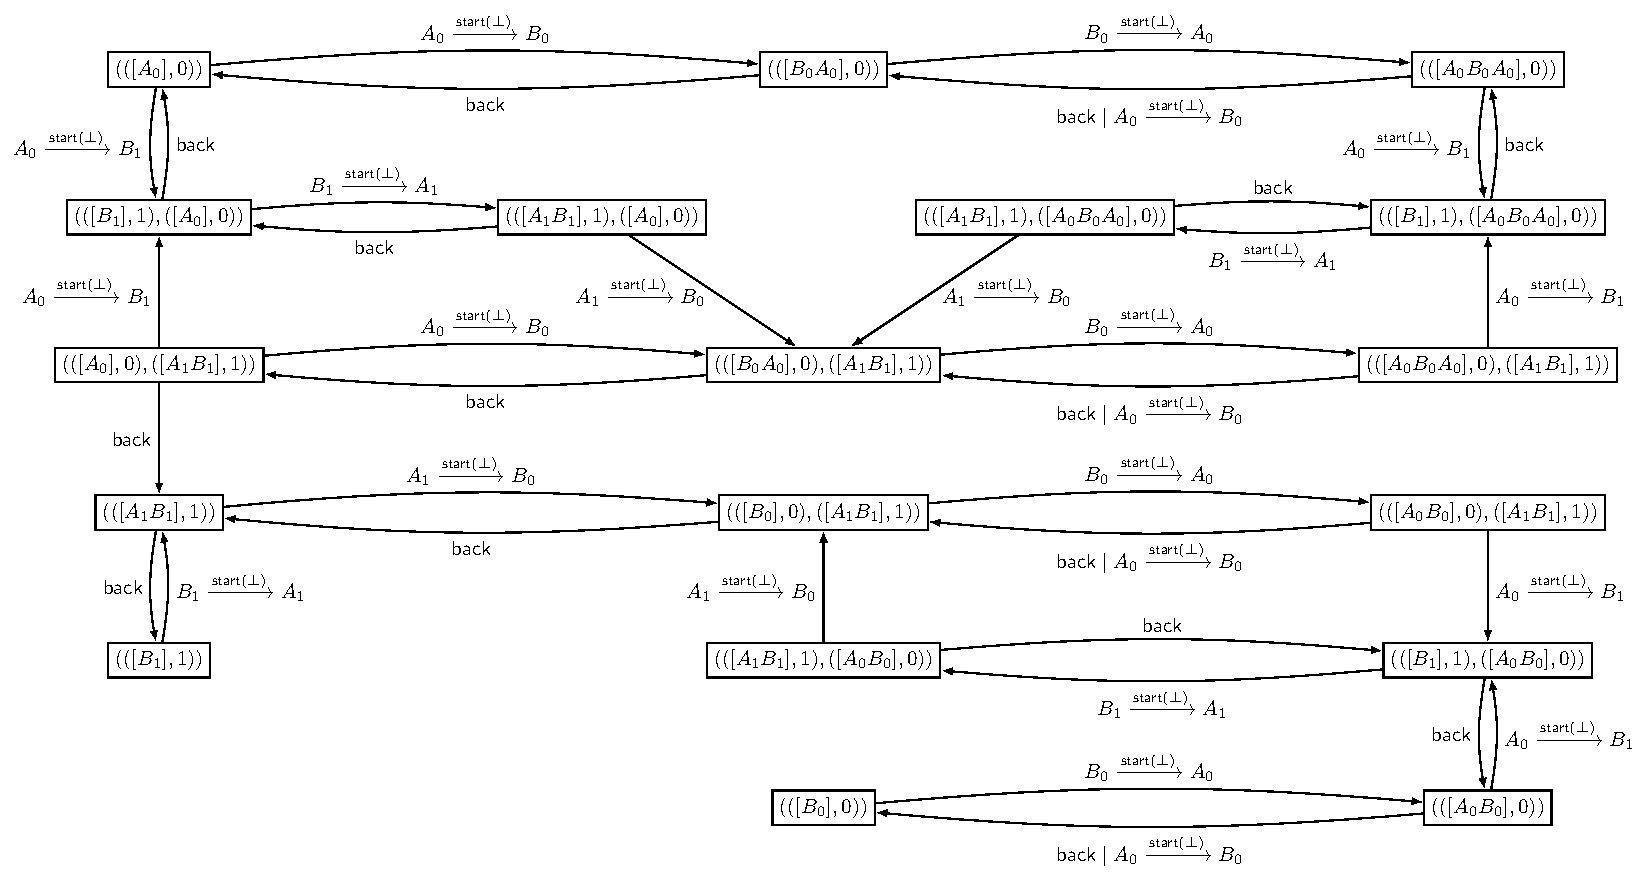
\includegraphics[scale = 0.55]{stk-lmasm-example.pdf}
			\caption{Configurations reachable from the initial configuration $(([A_0], 0))$ in the $\STK$-dominating $\LMAMASS$ $\Mm_{\textsf{LM}}$}
				%in $\phi$
		% \vspace{-6mm}	
		\label{stk-lmasm-example}
	\end{figure}

Let $\Mm_{\textsf{IF}}=(\act_{\textsf{IF}},A,\lmd_{\textsf{IF}},\aft_{\textsf{IF}},\Delta_{\textsf{IF}})$ be an $\STK$-dominating $\IFAMASS$, where $\act_{\textsf{IF}} = \{A, B\}$, and $\lmd_{\textsf{IF}}(A) = \lmd_{\textsf{IF}}(B) = \STD$, $\aft_{\textsf{IF}}(A) = \lmd_{\textsf{IF}}(B) = 1$.
	Moreover, $\Delta_{\textsf{IF}} = \{\back, \tau_1, \tau_2, \tau_3 \}$, where 
	$\tau_1 = A\xrightarrow[]{\startactivity(\bot)}B$,
	$\tau_2 = B\xrightarrow[]{\startactivity(\bot)}A$,
	$\tau_2 = B\xrightarrow[]{\startactivity(\rtfflag)}A$.
	Then the configurations that are reachable from the initial configuration $[A]$ by executing the transition rules from $\Delta_{\textsf{IF}}$ are illustrated in Figure~\ref{stk-ifasm-example}, where the vertices denote the configurations and the edges denote the elements of $\xrightarrow[\Mm_{\textsf{IF}}]{}$. 
	For instance, 
	\begin{itemize}
	\item if $B \xrightarrow{\startactivity(\rtfflag)} A$ is applied to the configuration $[B]$, then $A$ is pushed to the task, since $\phi\models\rtfflag$ and $A$ dose not occur in the task $[B]$, resulting to the configuration $[AB]$,
	%
	\item if $B \xrightarrow{\startactivity(\rtfflag)} A$ is applied to the configuration $[BA]$, then $A$ is moved to the top of the task, since $\phi\models\rtfflag$ and $A$ occurs in the task $[BA]$, resulting to the configuration $[AB]$,
	%
	\item if $B \xrightarrow{\startactivity(\rtfflag)} A$ is applied to the configuration $[BABA]$, then the topmost $A$ is moved to the top of the task, since $\phi\models\rtfflag$ and $A$ occurs in the task $[BABA]$, resulting to the configuration $[ABBA]$,
	%

	\end{itemize}
	Note that for $\Mm_{\textsf{IF}}$, there are infinite many configurations reachable from the initial configuration. Therefore, we will only display configurations with a length no greater than $4$.

	\begin{figure}
		% \vspace{-3mm}
			\centering
			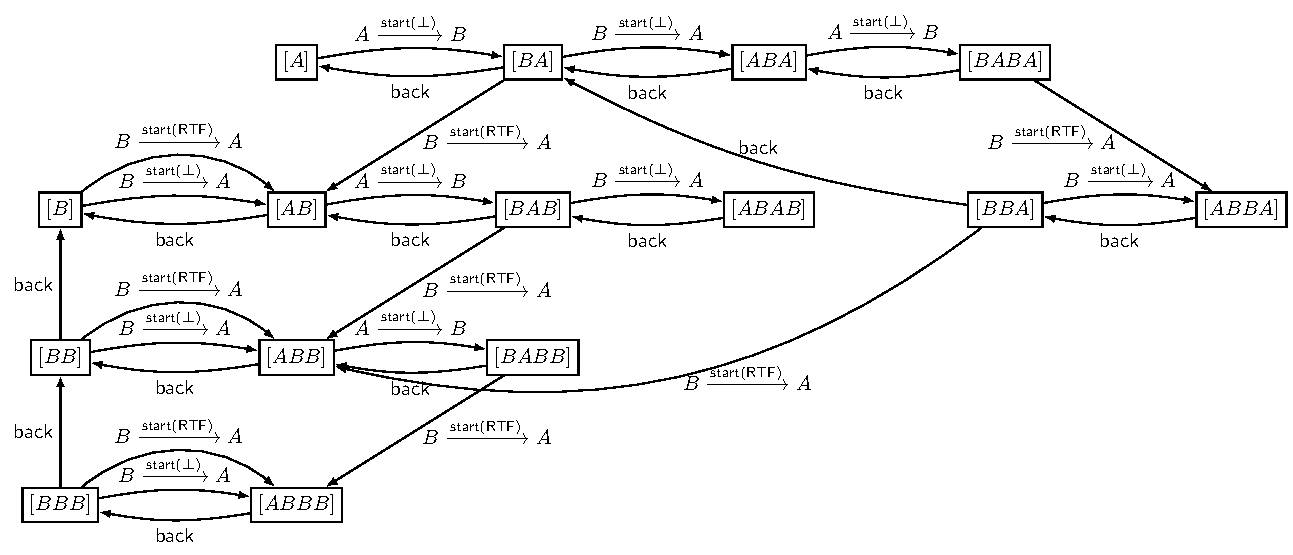
\includegraphics[scale = 0.65]{stk-ifasm-example.pdf}
			\caption{Configurations reachable from the initial configuration $[A]$ in the $\STK$-dominating $\IFAMASS$ $\Mm_{\textsf{IF}}$}
				%in $\phi$
		% \vspace{-6mm}	
		\label{stk-ifasm-example}
	\end{figure}

Let $\Mm=(\act_{\textsf{LM}},A_0,\lmd_{\textsf{LM}},\aft_{\textsf{LM}},\Delta)$ be an $\STK$-dominating $\AMASS$, where $\Delta = \{\back,\tau_1, \tau_2, \tau_3, \tau_4, \tau_5\}$, where 
		$\tau_1 = A_0 \xrightarrow{\startactivity(\bot)} A_1$,
		$\tau_2 = A_1 \xrightarrow{\startactivity(\bot)} B_0$,
		$\tau_3 = B_0 \xrightarrow{\startactivity(\rtfflag)} A_1$,
		$\tau_4 = A_1 \xrightarrow{\startactivity(\bot)} B_1$,
		$\tau_5 = B_1 \xrightarrow{\startactivity(\bot)} B_0$.
	Then the configurations that are reachable from the initial configuration $(([A_0], 0))$ by executing the transition rules from $\Delta$ are illustrated in Figure~\ref{stk-asm-example}, where the vertices denote the configurations and the edges denote the elements of $\xrightarrow[\Mm]{}$. 
	For instance, 
	\begin{itemize}
	\item if $B_0 \xrightarrow{\startactivity(\rtfflag)} A_1$ is applied to the configuration $(([B_0A_1A_0],0),([B_1],1))$, then $A_1$ is moved to the top of the top task $([B_0A_1A_0],0)$, since $\phi\models\rtfflag$ and $\lmd_{\textsf{IF}}(A_1) = \STD$ and $A_1$ occurs in the task $([B_0A_1A_0],0)$, resulting to the configuration $(([A_1B_0A_0],0),([B_1],1))$,
	%
	\item if $A_1 \xrightarrow{\startactivity(\bot)} B_0$ is applied to the configuration $(([A_1B_0A_0],0),([B_1],1))$, then all the activities above $B_0$, which is $A_1$ here, are removed from the task $([A_1B_0A_0],0)$, since $\lmd_{\textsf{LM}}(B_0) = \STK$, 
	$$\gettsk((([A_1B_0A_0],0),([B_1],1)), B_0) = ([A_1B_0A_0],0)$$
	and $B_0$ occurs in the task $([A_1B_0A_0],0)$, resulting to the configuration $(([B_0A_0],0),([B_1],1))$,
	%
	\item if $B_1 \xrightarrow{\startactivity(\bot)} B_0$ is applied to the configuration $(([B_1],1),([A_1A_0], 0))$, then the task $([A_1A_0], 0)$ is moved to the top and $B_0$ is pushed to the task,
	since $\lmd_{\textsf{LM}}(B_0) = \STK$, 
	$$\gettsk((([B_1],1),([A_1A_0], 0)), B_0) = ([A_1A_0], 0)$$
	and $B_0$ dose not occur in the task $([A_1A_0], 0)$, resulting to the configuration $(([B_0A_1A_0],0),([B_1],1))$.
	\end{itemize}
	Note that for $\Mm$, there are only finitely many configurations reachable from the initial configuration, which may not be the case for $\STK$-dominating $\AMASS$ in general.  
	\begin{figure}
		% \vspace{-3mm}
			\centering
			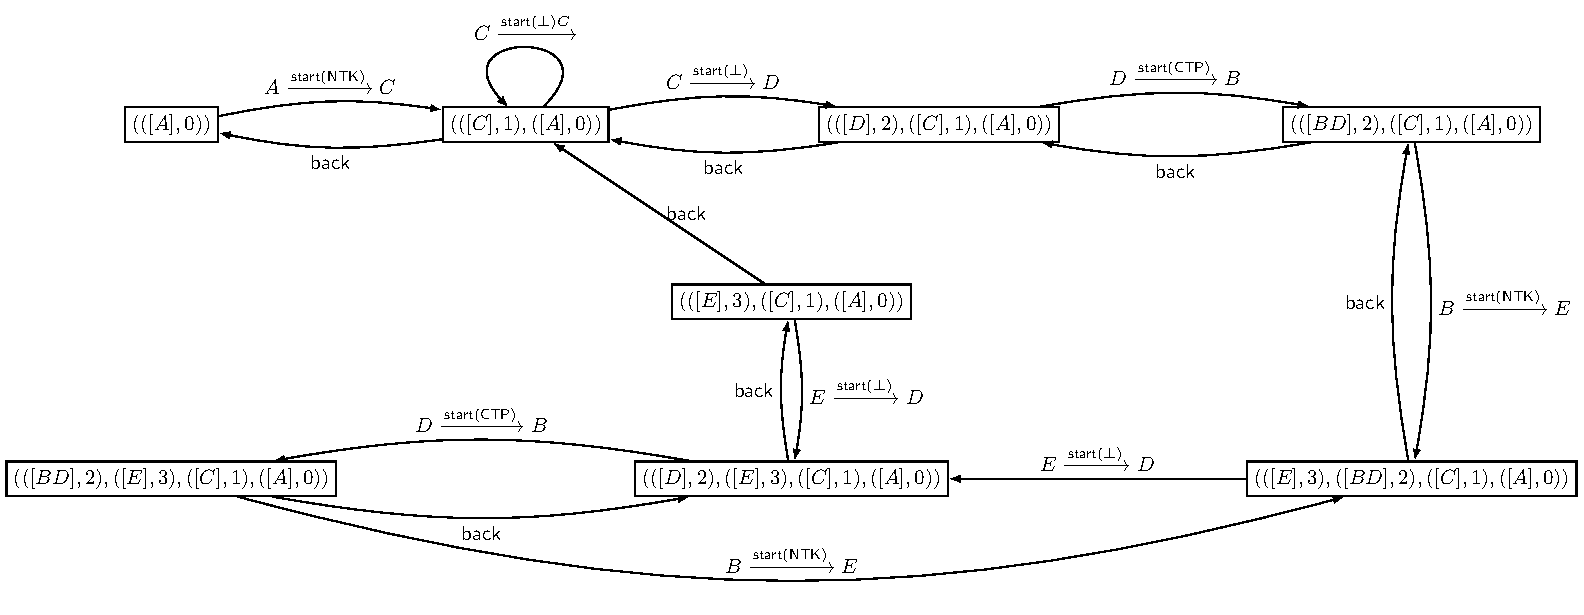
\includegraphics[scale = 0.6]{stk-asm-example.pdf}
			\caption{Configurations reachable from the initial configuration $(([A_0], 0))$ in the $\STK$-dominating $\AMASS$ $\Mm$}
				%in $\phi$
		% \vspace{-6mm}	
		\label{stk-asm-example}
	\end{figure}

% example of STK-dominating AMASS here. \zhilin{three examples for $\LMAMASS$, $\IFAMASS$, and $\AMASS$ respectively, to be used in the decision procedure.}
\end{example}


\begin{proposition}\label{prop-stk}
    Let $\Mm=(\act,A_0,\lmd,\aft,\Delta)$ be an $\STK$-dominating $\AMASS$. Then each configuration $\rho$ that is reached from the initial configuration $(([A_0],\aft(A_0)))$ in $\Mm$ satisfies the following constraints:
    \begin{enumerate}
        \item for each $\STK$-activity $A\in\act$ with $\aft(A)\neq\aft(A_0)$, $A$ can only occur at the bottom of some task in $\rho$, 
        \item $\rho$ contains at most one $\standard/\singletop$-task, which, when it exists, has the same affinity as $A_0$.
		% \item $\SIT$ activity has the same effects with $\STK$ activity.
    \end{enumerate}
\end{proposition}

We are ready to state the main result of this paper. 

\begin{theorem}\label{thm:st-amass-reach}
The configuration reachability problem of $\STK$-dominating $\AMASS$ is decidable.
\end{theorem}

The rest of this paper is devoted to the proof of Theorem~\ref{thm:st-amass-reach}. Since the decision procedure is involved, to ease the understanding, we present the decision procedure for $\singletask$-dominating $\LMAMASS$ first (Section~\ref{sec:reach-lmamass}), then $\singletask$-dominating $\IFAMASS$ (Section~\ref{sec:reach-ifamass}), and finally consider $\singletask$-dominating $\AMASS$ in its most general case (Section~\ref{sec:reach-amass}). 

For technical convenience, let us assume that \emph{the affinities of $\singleinstance$-activities are mutually distinct, moreover, they are different from those of the other activities}, that is, for each $A, B \in \act_\singleinstance$ with $A \neq B$, we have $\aft(A) \neq \aft(B)$, moreover, $\aft(\act_\singleinstance) \cap \aft(\act \setminus \act_\singleinstance) = \emptyset$. Note that this assumption is not a restriction, since regarding the task allocation mechanism, the affinities of $\singleinstance$-activities are redundant and independent of those of the other activities. With this assumption, the task allocation mechanism (formalized by $\gettsk(\rho, B)$) can be specified by the \emph{name function} $\namefun_B(\theta)$ defined in the sequel:  Let $\theta = \aname_1 \cdots \aname_k$ and $B \in \act$. Then $\namefun_B(\theta) = i$ if $\aft(B) = \aname_i$ for some $i \in [k]$, and $\namefun_B(\theta) = \bot$ otherwise. Note that the invariant of configurations, that is, the task affinities of every two non-$\singleinstance$ tasks are mutually distinct, guarantees the well-definedness of $\namefun_B(\theta)$.

%For simplicity, we assume that $\Mm$ contains $\standard$ and $\singletask$ activities only. 
%The proof of Theorem~\ref{thm:st-amass-reach} is technically the most challenging part of this paper. 
%To ease the understanding, we shall prove the configuration reachability problem of $\STK$-dominating $\LMAMASS$ (resp. $\STK$-dominating $\IFAMASS$) is decidable in Section~\ref{sec:reach-lmamass} (resp. Section~\ref{sec:reach-ifamass}) first, then prove the configuration reachability problem of $\STK$-dominating $\AMASS$ is decidable in Section~\ref{sec:reach-amass}.



\section{Configuration reachability problem of $\STK$-dominating $\LMAMASS$}\label{sec:reach-lmamass}
%!TEX root = main.tex

%Recall that the definition of $\STK$-dominating $\LMAMASS$, then we let $\tau= A\xrightarrow{\startactivity(\bot)}B$ and let $\rho = (S_1, \cdots, S_n)$ be the current configuration for some $n \ge 1$ and $\topact(\rho) = A$. 

%we define the semantics of $\STK$-dominating $\LMAMASS$ as follows:
%\begin{itemize}
%    \item If $\lmd(B) = \STD$, then $\rho' = \push(\rho, B)$,
%    \item If $\lmd(B) = \STK$, then 
%    \begin{itemize}
%        \item if $\gettsk(\rho, B) = S_i$ for some $i\in[n]$, then
%        \begin{itemize}
 %           \item if $B \not \in S_i$, then $\rho' = \push(\mvtsktop(\rho, i), B)$,
 %           \item if $B  \in S_i$, 	then $\rho' =  \clrtop(\mvtsktop(\rho, i), B)$,
 %       \end{itemize}
%    \item if $\gettsk(\rho, B) = *$, then $\rho' = \newtsk(\rho, B)$.
%    \end{itemize}
%\end{itemize}

Let us assume that $\Mm=(\act,A_0,\lmd,\aft,\Delta)$ is an $\singletask$-dominating $\LMAMASS$.

We show how to solve the configuration reachability problem of $\Mm$.  
Let $(\Aut_1,\cdots,\Aut_k)$ be an {\NFA} tuple over the alphabet $\act$, and $\theta = \aname_1\cdots\aname_k$ be an affinity sequence. 
Our goal is to decide whether there is a configuration $\rho$ that is reachable from the initial configuration and accepted by $(\theta, (\Aut_1,\cdots,\Aut_k))$.
% satisfying that for each $i\in[k]$, $\aname_i=\aname_i'$, $S_i\in\ConfSet(\Aut_i)$, moreover, $(([A_0],\aft(A_0)))\xRightarrow[\Mm]{}\rho$.

The main idea is to show that the set of configurations that are reachable from the initial configuration can be represented finitely as recognizable relations defined in the sequel. 

\begin{definition}[Recognisable relations]
A $k$-ary string relation $R \subseteq (\act^*)^k$ is \emph{recognisable}  if it is a finite union of products of regular languages, that is, $R=\bigcup \limits_{i =1 }^n L_{i,1} \times \cdots \times L_{i, k}$, where each $L_{i,j}$ is a regular language. An {\NFA}-representation of $R$ is $\{(\Aut_{i,1},\cdots,\Aut_{i,k})\}_{i\in[n]}$, where each $\Aut_{i,j}$ is an {\NFA} defining $L_{i,j}$, that is, $\Lang(\Aut_{i,j}) = L_{i,j}$.
\end{definition}

%Our approach to tackle this case is to simulate the behaviors of a single task by a {\PDS}, and use a set of {\NFA} tuples to represent the configurations of {\AMASS} $\Mm$.
%Theorem~\ref{thm:iff-recog} shows the reachability problem of $\STK$-dominating $\LMAMASS$ is decidable, and we prove Theorem~\ref{thm:iff-recog} by Lemma~\ref{lem:iff-forward} and Lemma~\ref{lem:iff-backward}.

Let $\Theta_\Mm = \left \{ \aname_1 \cdots \aname_k \in (\aft(\act))^+ \mid k \le |\act_{\singleinstance}| + |\aft(\act)| \right\}$. Intuitively, $\Theta_\Mm$ denotes the set of affinity sequences  in the configurations of $\Mm$. For each $\theta=\aname_1 \cdots \aname_k \in \Theta_\Mm$, we define 
%
$$
\begin{array}{l}
\RLang(\Mm, \theta) = \\
\ \ \left\{(S_1, \cdots, S_k) \in (\aft^+)^k\ \big{\vert}\  ([A_0], \aft(A_0)) \xRightarrow[\Mm]{} ((S_1, \aname_1), \cdots, (S_k, \aname_k)) \right\}.
\end{array}
$$ 
%
Since each task $S_i$ can be seen as a string from $\act^+$, $\RLang(\Mm, \theta)$ can be seen as a $k$-ary string relation over $\act^+$. 


\begin{lemma}\label{lem:iff-recog}
    For each $\theta \in \Theta_\Mm$, $\RLang(\Mm, \theta)$ is a recognizable relation and its $\NFA$-representation can be effectively computed.
\end{lemma} 
% We solve the reachability problem in this case by deciding whether there is a {\WOTrNFA}-representation $(\theta,(\Aut_1,\cdots,\Aut_k))$ of $\conf_{\theta}$ for $\theta\in\Theta_{\Mm}$, satisfying $\Aut_i\cap\Aut_i\neq\emptyset$ for each $i\in[k]$ with $\ConfSet(\Aut_i) = \ConfSet_i$.

According to Lemma~\ref{lem:iff-recog}, for each $\theta = \aname_1 \cdots \aname_k \in \Theta_\Mm$, an {\NFA}-representation of $\RLang(\Mm, \theta)$, say $(\Aut_{\theta, i,1},\cdots,\Aut_{\theta, i,k})_{i \in [n_\theta]}$, can be effectively computed. 
Then the configuration reachability problem of $\Mm$ is solved as follows: If there is $\theta =  \aname_1 \cdots \aname_k \in \Theta_\Mm$ such that $\Lang(\Aut_{\theta, i, j}) \cap \Lang(\Aut_j) \neq \emptyset$ for each $j \in [k]$, then report ``yes'', otherwise, report ``no''.

% The rest of this section is devoted to the proof of Theorem~\ref{thm:iff-recog}.
The rest of this section is devoted to the proof of Lemma~\ref{lem:iff-recog}. We shall distinguish whether $\lmd(A_0) = \STK$ or not. 
The former case is simpler because, by Proposition~\ref{prop-stk}, all tasks will be rooted at $\STK$ activities. For the latter, the more general case, the back stack may contain, apart from the tasks rooted at $\STK$ activities, one single task rooted at $A_0$. 
We shall consider the two cases in Section~\ref{sec:lmamass-stk} and Section~\ref{sec:lmamass-nostk} respectively.

%Let us introduce a notation. 


\subsection{The case $\lmd(A_0) = \STK$}\label{sec:lmamass-stk}

In this case, we prove Lemma~\ref{lem:iff-recog} by showing that the set of configurations that are reachable from the initial configuration can be \emph{saturated by repeatedly applying a finite set of rules}. 

Before presenting the rules, let us introduce several notations. 

Let $A \in \act_\singletask\cup\act_{\singleinstance}$. 
We define a {\PDS} $\Pp_{A} = (P, \Gamma_{A}, \Delta_{A})$, where 
\begin{itemize}
\item $P = \{p_0, p_{\pop}\}$, 
\item $\Gamma_{A} = \act_{\standard}\cup\act_{\singletop}\cup\{A\}$ if $\lmd(A) = \singletask$, $\Gamma_{A} = \{A\}$ otherwise.
\item $\Delta_{A}$ is defined as follows: 
\begin{itemize}
%\item $(p_1, A, p_1) \in \Delta_A$. 
%
\item For each activity $A' \in \Gamma_A $, we have $(p_0, A', \epsilon, p_0) \in \Delta_{A}$.
%
\item For each transition rule $A' \xrightarrow{\startactivity(\bot)} A'' \in \Delta$ such that $\lmd(A') \neq \singleinstance$ and $\lmd(A'') \neq  \singleinstance$, 
\begin{itemize}
    \item if either $\lmd(A'') = \STD$ or $\lmd(A'') = \singletop$ and $A' \neq A''$, we have $(p_0, A', A''A', p_0) \in \Delta_{A}$,    
    % \item For each transition $A\xrightarrow{\startactivity(\bot)}B\in\Delta$, if $\lmd(B) = \STP$ and $A\neq B$, then $(p_0, A, BA, p_0)\in\Delta_{A'}$,
    \item if $\lmd(A) = \singletask$, $A' \neq A$ and $A'' = A$, then $(p_0, A', \epsilon, p_{\pop}) \in \Delta_{A}$, and for each $B \in \Gamma_{A} \setminus \{A\}$, $(p_{\pop}, B, \epsilon, p_{\pop}) \in \Delta_{A}$, moreover, $(p_{\pop}, A, A, p_0) \in \Delta_{A}$. (Intuitively, these transition rules simulate the action of popping the task until reaching an instance of $A$. )
\end{itemize}
\end{itemize}
Note that in the definition of $\Delta_{A}$, the transition rules $A' \xrightarrow{\startactivity(\bot)} A'' \in \Delta$ satisfying the following condition are ignored: $\lmd(A') = \singleinstance$, or $\lmd(A'') = \singleinstance$, or $\lmd(A'') = \singletask$ and $A'' \neq A$. 
Moreover, if $\lmd(A) = \singleinstance$, according to the definition of $\STK$-dominating $\LMAMASS$ and $\Pp_A$, we know that $\Delta_A = \{(p_0,A,\epsilon,p_0)\}$.
\end{itemize}
Intuitively, $\Pp_{A}$ simulates the behavior of a task of $\Mm$ where $A$ is already in the bottom of the task. 


%By slightly abusing the notation, for a $\Pp_{A}$-{\NFA} $\Aut$ where $p_0$ is the only initial state, let us use $\Lang(\Aut)$ to denote $w \in \act^+$ such that $(p_0, w) \in \conf_{\Aut}$. 
In the sequel, we define the $\Pp_{A}$-{\NFA}s $\Aut_{A}$ and $\Aut_{A\rightsquigarrow B}$ for $B \in \Gamma_A$ such that $\Lang(\Aut_A) = \{A\}$ and $\Lang(\Aut_{A\rightsquigarrow B}) =B\act^* \cap \Lang((\Aut_{A})^{\post^*}_{\Pp_A})$. 
\begin{itemize}
    \item $\Aut_{A} = (P', \Gamma_A, \{(p_0, A, p_f)\},\{p_0\},\{p_f\} )$, where $P' = P \cup \{p_f\} \cup \{\langle p_0,A'\rangle \mid A'\in\Gamma_A\}$ with $p_f \not \in P$.  
    %
    \item For $B \in \Gamma_A$, $\Aut_{A\rightsquigarrow B}$ is obtained from $(\Aut_{A})^{\post^*}_{\Pp_A}$ by \emph{removing all non-$B$ transitions out of $p_0$}, then removing all transitions that cannot be reached from $p_0$. 
\end{itemize}
Note that it is possible that $\Lang(\Aut_{A\rightsquigarrow B}) = \emptyset$.
From the definition of $\Pp_A$, $\Aut_A$, and $\Aut_{A\rightsquigarrow B}$, we know that $\Lang((\Aut_A)^{\post^*}_{\Pp_A}) = \bigcup\limits_{B\in\Gamma_A} \Lang(\Aut_{A\rightsquigarrow B})$ and $\Lang(\Aut_{A\rightsquigarrow A}) = \Lang(\Aut_A)$. 
%Note that for each $S\in\ConfSet(\Aut_A^B)$, we have $\btmact(S) = A$.

%The main idea is to show that the set of configurations that are reachable from the initial configurations can be 

%
%We start with a simpler case, i.e., $\lmd(A_0)=\STK$. Intuitively, for a configuration $\rho = (S_1,\cdots,S_k)$, there is an {\NFA}-representation $(\Aut_1,\cdots,\Aut_k)$ in $\AutReach$ satisfying that $S_i\in\ConfSet(\Aut_i)$ for each $i\in[k]$. From the Proposition~\ref{prop-stk}, we know each task $S_i$ is rooted at an $\STK$-activity which sits on the bottom of $S_i$. Suppose $\topact(S_1) = A$. When a transition $A\xrightarrow{\startactivity(\bot)}B$ with $B\in\act_{\STK}$ is fired, according to the semantics of $\Mm$, the $B$-task of $\rho$, say $S_i$, is switched to the top of $\rho$ and changed into $[B]$. To simulate this,  we add the tuple $(\Aut_i',\Aut_1,\cdots,\Aut_{i-1},\Aut_{i+1},\cdots,\Aut_k)$ into $\AutReach$ with $\ConfSet(\Aut_i') = [B]$.

We are ready to present the procedure that computes effectively $\AutReach$, a finite set of pairs $(\aname_1 \cdots \aname_k, (\Aut_1, \cdots, \Aut_k))$ where each of $\Aut_i$'s are of the form $\Aut_{A\rightsquigarrow B}$ for $A \in \act_\singletask\cup\act_\singleinstance$ and $B \in \Gamma_A$, by repeatedly applying a finite set of saturation rules, such that
\[\RConfs(\Mm) = \bigcup \limits_{(\aname_1 \cdots \aname_k, (\Aut_1, \cdots, \Aut_k)) \in \AutReach} \confs((\aname_1 \cdots \aname_k, (\Aut_1, \cdots, \Aut_k))).\]

Initially, let $\AutReach := \{(\aft(A_0),(\Aut_{A_0}))\}$.
Then it adds pairs to $\AutReach$, according to the following saturation rules, until no more pairs can be added. 

\smallskip
\fbox
{
\begin{minipage}{0.9\textwidth}
\begin{enumerate}
    %
    \item If $A \xrightarrow{\startactivity(\bot)}A' \in\Delta$, $\lmd(A')=\STK$ or $\singleinstance$, $(\theta, (\Aut_1,\cdots,\Aut_k)) \in \AutReach$ such that $\Lang(\Aut_1) \neq \emptyset$ and $\Aut_1 = \Aut_{B\rightsquigarrow A}$ for some $B \in \act_\singletask\cup\act_\singleinstance$, moreover, $\namefun_{A'}(\theta) = \bot$,
    then let $\AutReach: = \AutReach \cup \{(\aft(A')\theta, (\Aut_{A'},\Aut_1,\cdots,\Aut_k))\}$.
    % where $\Aut_1'$ is obtained from $\Aut_1$ by 
    % removing all non-$A$ transitions out of $p_0$, then removing all transitions cannot be reached from $p_0$.
        \textbf{[launch an $A'$-task]}

    \item If $A \xrightarrow{\startactivity(\bot)}A' \in\Delta$, $\lmd(A')=\STK$ or $\singleinstance$, $(\theta, (\Aut_1,\cdots,\Aut_k)) \in \AutReach$ such that $\Lang(\Aut_1) \neq \emptyset$ and $\Aut_1 = \Aut_{B\rightsquigarrow A}$ for some $B \in \act_\singletask\cup\act_\singleinstance$, moreover, $\namefun_{A'}(\theta) = i$ for some $i \in [k]$ with $i > 1$, 
        then let $\AutReach:= \AutReach \cup \{(\theta', (\Aut_{A'}, \Aut_1, \cdots,\Aut_{i-1},\Aut_{i+1},\cdots,\Aut_{k}))\}$, where $\theta' = \aname_i\aname_1\dots\aname_{i-1}\aname_{i+1}\dots\aname_k$. 
        % and $\Aut_1'$ is obtained from $\Aut_1$ by removing all non-$A$ transitions out of $p_0$, then removing all transitions cannot be reached from $p_0$.
        \textbf{[escalate the $A'$-task to be the top and reset its content to $[A']$]}
        %
    \item If $(\aname_1 \cdots \aname_k, (\Aut_1,\cdots,\Aut_k)) \in \AutReach$ and $k>1$, then let $\AutReach := \AutReach \cup \{(\aname_2\dots\aname_k, (\Aut_2,\cdots,\Aut_k))\}$.
        \textbf{[pop all activities in the top task]}
%
    \item If $(\theta, (\Aut_1,\cdots,\Aut_k)) \in \AutReach$, $\Aut_1 = \Aut_{A\rightsquigarrow B}$ for some $A\in\act_{\STK}\cup\act_{\SIT}$ and $B \in \Gamma_A$, and $B'  \in \Gamma_A$ such that $\Lang(\Aut_{A\rightsquigarrow B'}) \neq \emptyset$, then let 
    $\AutReach := \AutReach \cup \{(\theta, (\Aut_{A\rightsquigarrow B'}, \Aut_2,\cdots,\Aut_k))\}$. 
    % then adds the tuple $(\theta, (\Aut_1^{\post^*},\Aut_2,\cdots,\Aut_k))$ to $\AutReach$.
%    such that $\Aut_1 = \Aut_A^B$ for some $A\in\act_{\STK},B\in\act$, then adds the tuple $(\theta, (\Aut_A^{B'},\Aut_2,\cdots,\Aut_k))$ to $\AutReach$ for each $B'\in\act$ with $\ConfSet(\Aut_A^{B'})\neq\emptyset$.
        \textbf{[simulate the behaviors of the top task]}
\end{enumerate}
\end{minipage}
}

\medskip

The aforementioned procedure terminates since $\Theta_\Mm$ is finite and the set of {\NFA}s $\Aut_{A\rightsquigarrow B}$ occurring in $\AutReach$ is finite.
Let $\AutReach_f$ denote the value of $\AutReach$ when the aforementioned procedure terminates. 




%We are going to present a procedure to compute the {\NFA}-representations of $\conf_\theta$ for $\theta \in \Theta_\Mm$. Specifically, the procedure computes a set of tuples $(\aname_1 \cdots \aname_k, (\Aut_1, \cdots, \Aut_k))$, denoted by $\AutReach$, such that for each $\theta =  \aname_1 \cdots \aname_k$, the {\NFA}-tuples $(\Aut_1, \cdots, \Aut_k)$ with $(\theta, (\Aut_1, \cdots, \Aut_k)) \in \AutReach$ constitute an {\NFA}-representation of $\conf_\theta$. 

% Moreover, all these {\NFA}s in $\AutReach$ are satisfied that the states are from $Q$, $p_1$ (resp. $p_f$) is the only initial (resp. final) state.

% To compute $\AutReach$, we need an additional notation $\topact_{A}(\Aut)$ for a $\Pp_{A}$-{\NFA} $\Aut$, an activity $A\in\act$ and we require that $\ConfSet(\Aut)\cap\ConfSet(A\act^*)\neq\emptyset$. Moreover we have $\ConfSet(\topact_{A}(\Aut)) = \ConfSet(\Aut)\cap\ConfSet(A\act^*)$, and $\topact_{A}(\Aut)$ could be obtained from $\Aut$ by removing all non-$A$ transitions out of $p_1$, then removing all transitions cannot be reached from $p_1$.
% which intuitively specifies how to obtain a new {\NFA} from $\Aut$ 
% when an $\STK$ activity $A$ is started. Moreover, we let $\Aut = (Q', \act, \delta, \{p_b\}, \{p_f\})$ for some $b\in\{0,1\}$, and we let all transitions out of $p_b$ are labeled with $B$, hence all strings accepted by $\Aut$ must (resp. \emph{not}) contain $A_0'$, if $b = 0$ (resp. $b=1$) and started with $B$.
% Then we define 


%Moreover, all these {\NFA}s in $\AutReach$ are in form $\Aut_A^B$ for some $A\in\act_{\STK}, B\in\act$. 

%For each $\theta=\aname_1\dots\aname_k\in\Theta_{\Mm}$ and an $\NFA$-tuple $(\Aut_1, \cdots, \Aut_k)$, we use $\Lang(\theta, (\Aut_1, \cdots, \Aut_k))$ to denote the set of $(S_1, \cdots, S_k) \in (\act^+)^k$ such that $((S_1, \aname_1), \cdots, (S_k, \aname_k)) \in \confs((\theta, (\Aut_1, \cdots, \Aut_k)))$.

We are going to prove Lemma~\ref{lem:iff-recog} for the case $\lmd(A_0) = \singletask$, that is, for each $\theta=\aname_1\dots\aname_k\in\Theta_{\Mm}$, 
%
\[\RLang(\Mm, \theta) = \bigcup \limits_{(\theta, (\Aut_1, \cdots, \Aut_k)) \in \AutReach_f} \Rel((\Aut_1, \cdots, \Aut_k)).\]

We prove the equation by showing the left-hand side is a subset of the right-hand side and vice versa. 

\paragraph*{The proof of $\RLang(\Mm, \theta) \subseteq \bigcup \limits_{(\theta, (\Aut_1, \cdots, \Aut_k)) \in \AutReach_f} \Rel((\Aut_1, \cdots, \Aut_k))$}

%\begin{lemma}\label{lem:iff-forward}
%    Let $\AutReach$ be the set computed by the aforementioned saturation procedure. Then for each $\theta=\aname_1\dots\aname_k\in\Theta_{\Mm}$, we have
%    $$\conf_{\theta}\subseteq\bigcup \limits_{(\theta, (\Aut_1, \dots, \Aut_k)) \in \AutReach} \ConfSet(\Aut_1) \times \dots \times \ConfSet(\Aut_k).$$
%\end{lemma}

%\begin{lemma}\label{lem:iff-forward}
%    Let $\AutReach$ be the set computed by the aforementioned saturation procedure. Then for each $\theta=\aname_1\dots\aname_k\in\Theta_{\Mm}$, we have
%    $$\conf_{\theta}\subseteq\bigcup \limits_{(\theta, (\Aut_1, \dots, \Aut_k)) \in \AutReach} \ConfSet(\Aut_1) \times \dots \times \ConfSet(\Aut_k).$$
%\end{lemma}

\begin{proof}
For $n \ge 1$, let $\xrightarrow[\Mm]{}^n$ denote the $n$-fold composition of $\xrightarrow[\Mm]{}$. Moreover, by convention, let $\xrightarrow[\Mm]{}^0$ be the identity relation on $\confs(\Mm)$. 
Then for each $\theta = \aname_1 \dots \aname_k \in \Theta_\Mm$, we prove by an induction on $n \ge 0$ the following claim.

\smallskip

\noindent {\bf Claim}. \emph{For each $n \ge 0$ and configuration $\rho =  ((S_1, \aname_1), \cdots, (S_k, \aname_k))$ such that 
%
$([A_0], \aft(A_0)) \xrightarrow[\Mm]{}^n \rho$,  let $\theta  = \aname_1 \cdots \aname_k$, then 
%
there is  $(\Aut_1, \dots, \Aut_k)$ such that $(\theta, (\Aut_1, \dots, \Aut_k)) \in \AutReach_f$ and $(S_1, \cdots, S_k) \in \Rel((\Aut_1,\cdots, \Aut_k))$}.   

%$\rho \in  \ConfSet(\Aut_1) \times \dots \times \ConfSet(\Aut_k)$.

\smallskip

\noindent \emph{Induction base $n = 0$}. From $([A_0], \aft(A_0)) \xrightarrow[\Mm]{}^0 \rho$, we have $\rho = ([A_0], \aft(A_0))$. From the computation of $\AutReach_f$, we know that $(\aft(A_0), (\Aut_{A_0})) \in \AutReach_f$. Since $[A_0] \in \Lang(\Aut_{A_0})$, the claim holds for $n = 0$. 

\smallskip

\noindent \emph{Induction step $n > 0$}. Suppose the claim holds for $n-1$. Assuming $([A_0], \aft(A_0)) \xrightarrow[\Mm]{}^n \rho =  ((S_1, \aname_1), \dots, (S_k, \aname_k))$, we are going to show that there is  $(\theta, (\Aut_1, \dots, \Aut_k)) \in \AutReach_f$ such that $(S_1, \cdots, S_k) \in \Rel((\Aut_1,\cdots, \Aut_k))$, that is, $S_i \in \Lang(\Aut_i)$ for each $i \in [k]$. 

From $([A_0], \aft(A_0)) \xrightarrow[\Mm]{}^n \rho$,  we know that there are a configuration $\rho' = ((S'_1, \aname'_1), \dots, (S'_l, \aname'_l))$ and a transition rule $\tau$ such that $([A_0]) \xrightarrow[\Mm]{}^{n-1} \rho' \xrightarrow[\Mm]{\tau} \rho$.

Let $\theta'= \aname'_1 \cdots \aname'_l$. Then from the induction hypothesis, there exists $(\theta', (\Aut'_1, \dots, \Aut'_l)) \in \AutReach_f$ such that $S'_j \in \Lang(\Aut'_j)$ for each $j \in [l]$. Moreover, let $A \in \act_\singletask\cup\act_\singleinstance$ and $B \in \Gamma_A$ such that $\Aut'_1 = \Aut_{A \rightsquigarrow B}$. 

If $\tau = \back$, then we distinguish between whether $|S'_1| > 1$ or not. 
\begin{itemize}
\item If $|S'_1| > 1$, then $\theta' = \theta$, $k=l$, $S'_1 = [B] \cdot S_1$, and $(S'_2, \cdots, S'_l) = (S_2, \cdots, S_k)$. 
Therefore, $S_1 \in \Lang(\Aut_{A \rightsquigarrow B'})$ for some $B'$. According to the 4th saturation rule, $(\theta, (\Aut_{A \rightsquigarrow B'}, \Aut'_1, \cdots, \Aut'_l)) \in \AutReach_f$. Since $(S_1, \cdots, S_k) \in \Rel((\Aut_{A \rightsquigarrow B'}, \Aut'_2, \cdots, \Aut'_l))$, we conclude that the claim holds for $n$ in this situation. 
%
\item If $|S'_1| = 1$, then $k = l - 1$, and $(S_1,\cdots,S_k) = (S_2',\cdots,S_l')$. According to the 3rd saturation rule, $(\theta, (\Aut_2',\cdots,\Aut_l')) \in \AutReach_f$. From $(S_1,\dots,S_k) = (S'_2, \cdots, S'_l) \in \Lang(\Aut_2') \times \cdots \times \Lang(\Aut_l') = \Rel((\Aut'_2, \cdots, \Aut'_l))$, we conclude that the claim holds for $n$ in this situation. 
\end{itemize}


Let us assume $\tau = B \xrightarrow{\startactivity(\bot)} C$ in the sequel. From the definition of $\singletask$-dominating $\AMASS$, there are the following three cases. 
\begin{itemize}
\item $\lmd(B) \neq \singleinstance$ and $\lmd(C) = \standard$ or $\singletop$, 
%
\item $\lmd(B) \neq \singleinstance$ and $\lmd(C) = \singletask$ or $\singleinstance$, 
%
\item $\lmd(B) = \singleinstance$ and $\lmd(C) = \singletask$ or $\singleinstance$. 
\end{itemize}

\smallskip

\noindent \emph{Case $\lmd(B) \neq \singleinstance$ and $\lmd(C) = \standard$ or $\singletop$}. In this case, $\theta = \theta'$. Moreover, $\rho = \rho'$ or $\rho$ is obtained from $\rho'$ by pushing $C$ to the top task.

If $\rho = \rho'$, then we are done. 

If $\rho$ is obtained from $\rho'$ by pushing $C$ to the top task, then $S_1 \in \Lang(\Aut_{A \rightsquigarrow C})$. Moreover, from the 4th saturation rule, we know that $(\theta, (\Aut_{A \rightsquigarrow C}, \Aut'_2, \cdots, \Aut'_l)) \in \AutReach_f$. 
Since 
$$(S_1, \cdots, S_k) \in \Lang(\Aut_{A \rightsquigarrow C}) \times \Lang(\Aut'_2) \times \cdots \times \Lang(\Aut'_l) = \Rel(\Aut_{A \rightsquigarrow C}, \Aut'_2, \cdots, \Aut'_l),$$ 
we conclude that the claim holds for $n$ in this case. 

\smallskip

\noindent \emph{Case $\lmd(B) \neq \singleinstance$ and $\lmd(C) = \singletask$ or $\singleinstance$}. 

If $C = A$, then $S_1 = [A]$. From the 4th saturation rule, $(\Aut_{A \rightsquigarrow A} = \Aut_A, \Aut'_2, \cdots, \Aut'_l) \in \AutReach_f$. Since $(S_1, \cdots, S_k) \in \Rel((\Aut_A, \Aut'_2, \cdots, \Aut'_l))$, we conclude that the claim holds for $n$ in this case. 

Let us assume $C \neq A$ in the sequel.  Then $\theta' \neq \theta$.  We distinguish between the following two subcases. 
\begin{itemize}
    \item \emph{Subcase $\namefun_{C}(\theta') = \bot$}. Then $k=l+1$, $S_1' \in \Lang(\Aut_{A\rightsquigarrow B})$, $S_1=[C]$, and $(S_2,\cdots,S_k)=(S_1',\cdots,S_l')$.  According to the 1st saturation rule, $(\theta, (\Aut_{C}, \Aut_1', \cdots, \Aut_l')) \in \AutReach_f$.
    %, where $\Lang(\Aut_1') \cap A\act^* \neq \emptyset$, and $S_1=[A']\in\ConfSet(\Aut_{A'})$, 
   From $(S_1, \cdots, S_k) = ([C], S_1', \cdots, S_l') \in \Lang(\Aut_{C}) \times \Lang(\Aut_1') \times \cdots \times \Lang(\Aut_l')$, we conclude that the claim holds for $n$ in this subcase.
    %
    \item \emph{Subcase $\namefun_{C}(\theta') = i \neq \bot$, and $i > 1$}: Then $k = l$, 
    $S'_1  \in \Lang(\Aut_{A\rightsquigarrow B})$, $S_1 = [C]$, $(S_2, \dots, S_k) = (S'_1, \dots, S'_{i-1}, S'_{i+1}, \dots, S'_l)$. According to the 2nd saturation rule, we know that $(\theta, (\Aut_{C}, \Aut_1',\cdots, \Aut_{i-1}', \Aut_{i+1}', \cdots, \Aut_{l}')) \in \AutReach_f$. 
%    where $\ConfSet(\Aut_1')\cap A\act^*\neq\emptyset$, and  $S_1=[A']\in\ConfSet(\Aut_{A'})$, 
    From 
    $$
    \begin{array}{l}
    	(S_1,\cdots,S_k) = ([C], S_1', \cdots, S_{i-1}', S_{i+1}', \cdots, S_l') \in \\
    	\ \ \Lang(\Aut_{C}) \times \Lang(\Aut_1') \times \cdots \times \Lang(\Aut_{i-1}') \times \Lang(\Aut_{i+1}')\times \cdots \times \Lang(\Aut_{l}'),
    \end{array}
    $$  
    we conclude that the claim holds for $n$ in this subcase. 
%
\end{itemize}

\smallskip

\noindent \emph{Case $\lmd(B) = \singleinstance$ and $\lmd(C) = \singletask$ or $\singleinstance$}. 

The discussion is similar to the previous case. 


%%%%%%%%%%%%%%%%%%% original proof removed
%%%%%%%%%%%%%%%%%%% original proof removed
\hide{
%Moreover, $\rho$ is obtained from $\rho'$ by a transition of $\Mm$. 
We distinguish between the cases $\theta' = \theta$ and $\theta' \neq \theta$.

\smallskip

\noindent \emph{Case $\theta' = \theta$}.
In this case, the configuration $\rho$ is obtained from $\rho'$ by only updating the content of the top task. 


% Moreover if $\lmd(A) = \singleinstance$ then we have $\rho = \rho'$, we know that the claim holds for $n$. Therefore we consider $\lmd(A)$
Therefore $(p_0,S_1')\xRightarrow{\Pp_{A}}(p_0,S_1)$, $l=k$, and $(S_2',\cdots,S_l')=(S_2,\cdots,S_k)$. 
%
%Let $\Aut'_1 = \Aut_{A, B}$ for some $A \in \act_\singletask$ and $B \in \act \setminus \act_\singleinstance$. 
From  $S'_1 \in \Lang(\Aut'_1)$, we have
%where we let $\Aut_1' = \Aut_A^B$ is a $\Pp_A$-{\NFA} for some $A \in \act_{\STK}, B\in\act$, 
$S_1 \in \Lang((\Aut_1')^{\post^*}_{\Pp_A})$. Moreover, from $\Lang(\Aut_1') = \Lang(\Aut_{A\rightsquigarrow B}) \subseteq \Lang((\Aut_A)^{\post^*}_{\Pp_A})$, we deduce $\Lang((\Aut_1')^{\post^*}_{\Pp_A}) \subseteq \Lang((\Aut_A)^{\post^*}_{\Pp_A})$. Therefore, $S_1 \in \Lang((\Aut_A)^{\post^*}_{\Pp_A})$. 

From $ \Lang((\Aut_A)^{\post^*}_{\Pp_A}) = \bigcup \limits_{B' \in \Gamma_A } \Lang(\Aut_{A\rightsquigarrow B'})$, we know that $S_1 \in \Lang(\Aut_{A\rightsquigarrow B'})$ for some $B'$. 
Furthermore, according to the aforementioned 4th saturation rule, we know that $(\theta, (\Aut_{A\rightsquigarrow B'}, \Aut_2', \cdots, \Aut'_l)) \in \AutReach_f$.
From $\rho = (S_1, \cdots, S_k) \in \Lang(\Aut_{A\rightsquigarrow B'}) \times \Lang(\Aut_2') \times \cdots \times \Lang(\Aut'_l)$, we know that the claim holds for $n$. 

\paragraph{Case $\theta' \neq \theta$}
In this case, the top task of $\rho$ is different from that of $\rho'$.  There are the following three subcases. 
\begin{itemize}
    \item \emph{Subcase $\tau = B \xrightarrow{\startactivity(\bot)} B'$, $\lmd(B') = \STK$ or $\SIT$, and $\namefun_{B'}(\theta') = \bot$}. Then $k=l+1$, $S_1' \in \Lang(\Aut_{A\rightsquigarrow B})$, $S_1=[B']$, and $(S_2,\cdots,S_k)=(S_1',\cdots,S_l')$.  According to the 1st saturation rule, $(\theta, (\Aut_{B'}, \Aut_1', \cdots, \Aut_l')) \in \AutReach_f$.
    %, where $\Lang(\Aut_1') \cap A\act^* \neq \emptyset$, and $S_1=[A']\in\ConfSet(\Aut_{A'})$, 
   From $(S_1, \cdots, S_k) = ([B'], S_1', \cdots, S_l') \in \Lang(\Aut_{B'}) \times \Lang(\Aut_1') \times \cdots \times \Lang(\Aut_l')$, we conclude that the claim holds for $n$ in this subcase.
    %
    \item \emph{Subcase $\tau = B \xrightarrow{\startactivity(\bot)} B'$, $\lmd(B')=\STK$ or $\SIT$, $\namefun_{B'}(\theta') = i \neq \bot$, and $i > 1$}: Then $k = l$, 
    $S'_1  \in \Lang(\Aut_{A\rightsquigarrow B})$, $S_1 = [B']$, $(S_2, \dots, S_k) = (S'_1, \dots, S'_{i-1}, S'_{i+1}, \dots, S'_l)$. According to the 2nd saturation rule, we know that $(\theta, (\Aut_{B'}, \Aut_1',\cdots, \Aut_{i-1}', \Aut_{i+1}', \cdots, \Aut_{l}')) \in \AutReach_f$. 
%    where $\ConfSet(\Aut_1')\cap A\act^*\neq\emptyset$, and  $S_1=[A']\in\ConfSet(\Aut_{A'})$, 
    From 
    $$
    \begin{array}{l}
    	(S_1,\cdots,S_k) = ([B'], S_1', \cdots, S_{i-1}', S_{i+1}', \cdots, S_l') \in \\
    	\ \ \Lang(\Aut_{B'}) \times \Lang(\Aut_1') \times \cdots \times \Lang(\Aut_{i-1}') \times \Lang(\Aut_{i+1}')\times \cdots \times \Lang(\Aut_{l}'),
    \end{array}
    $$  
    we conclude that the claim holds for $n$ in this subcase. 
%
    \item \emph{Subcase $\tau = \back$ and $|S_1'|=1$}. Then $k = l - 1$, and $(S_1,\cdots,S_k) = (S_2',\cdots,S_l')$.  According to the 3rd saturation rule, $(\theta, (\Aut_2',\cdots,\Aut_l')) \in \AutReach_f$. From $(S_1,\dots,S_k) = (S'_2, \cdots, S'_l) \in \Lang(\Aut_2') \times \cdots \times \Lang(\Aut_l')$, we conclude that the claim holds for $n$ in this subcase. 
\end{itemize}
}
%%%%%%%%%%%%%%%%%%% original proof removed
%%%%%%%%%%%%%%%%%%% original proof removed
\end{proof}


\paragraph*{The proof of $\bigcup \limits_{(\theta, (\Aut_1, \cdots, \Aut_k)) \in \AutReach_f}  \Rel((\Aut_1, \cdots, \Aut_k)) \subseteq \RRel(\Mm, \theta)$}

%\begin{lemma}\label{lem:iff-backward}
%    Let $\AutReach$ be the set computed by the aforementioned saturation procedure. Then for each $\theta = \aname_1 \dots \aname_k \in \Theta_\Mm$, we have 
%    $$\bigcup \limits_{(\theta, (\Aut_1, \dots, \Aut_k)) \in \AutReach} \ConfSet(\Aut_1) \times \dots \times \ConfSet(\Aut_k) \subseteq \conf_\theta.$$
%\end{lemma}

\begin{proof}
Since $\AutReach_f$ is computed by applying the saturation rules and adding the tuples into $\AutReach$,  let us use $\AutReach_0$ to denote $\{(\aft(A_0), \Aut_{A_0})\}$, use $\AutReach_1$ to denote the set obtained by adding a tuple to $\AutReach_0$, and for $n \ge 2$, use $\AutReach_n$ to denote the set obtained by adding a new tuple to $\AutReach_{n-1}$. 
We prove by an induction on $n \ge 0$ the following claim.  

\smallskip
\noindent {\bf Claim}. For each $n \ge 0$, if $(\theta, (\Aut_1, \cdots, \Aut_k)) \in \AutReach_n$ with $\theta = \aname_1 \cdots \aname_k$ and $(S_1,\dots,S_k) \in \Rel((\Aut_1, \cdots, \Aut_k))$, then $(([A_0], \aft(A_0))) \xRightarrow[\Mm]{} ((S_1, \aname_1), \cdots, (S_k, \aname_k))$.

\smallskip

%    Let $\AutReach_n$ be the set computed by the aforementioned saturation procedure after the $n$-th tuple $(\theta,(\Aut_1,\dots,\Aut_k))$ is added, 


\noindent \emph{Induction base $n = 0$}. 
Because $\AutReach_0 = \{(\aft(A_0),(\Aut_{A_0}))\}$, if $(S_1, \cdots, S_k) \in \Rel((\Aut_{A_0}))$, then $k=1$ and $S_1 = [A_0]$. Since $(([A_0], \aft(A_0))) \xRightarrow[\Mm]{} (([A_0], \aft(A_0)))$, it follows that the claim holds for $n = 0$. 

\smallskip

\noindent \emph{Induction step $n > 0$}. 
Suppose that $(\theta, (\Aut_1, \cdots, \Aut_k)) \in \AutReach_n$ with $\theta = \aname_1 \cdots \aname_k$ and $(S_1,\dots,S_k) \in \Rel((\Aut_1, \cdots, \Aut_k))$. 

If $(\theta, (\Aut_1, \cdots, \Aut_k)) \in \AutReach_{n-1}$, then the claim follows directly from the induction hypothesis. 

Next, let us assume that $(\theta, (\Aut_1, \cdots, \Aut_k)) \not \in  \AutReach_{n-1}$.
Therefore, $\AutReach_{n} = \AutReach_{n-1} \cup \{(\theta,(\Aut_1,\dots,\Aut_k))\}$.  
%
%Then the $n$-th tuple $(\theta,(\Aut_1,\dots,\Aut_k))$ is added which obtained from $(\theta',(\Aut_1',\dots,\Aut_l'))\in \AutReach_{n-1}$.
We distinguish which saturation rule is used to add $(\theta,(\Aut_1,\dots,\Aut_k))$.


\paragraph*{The 1st saturation rule} Then  there are a transition rule $\tau = A \xrightarrow{\startactivity(\bot)} A'  \in \Delta$ and $(\theta', (\Aut'_1, \cdots, \Aut'_l)) \in \AutReach_{n-1}$ such that $\lmd(A')=\STK$ or $\singleinstance$, $\Lang(\Aut'_1) \neq \emptyset$, $\Aut'_1 = \Aut_{B\rightsquigarrow A}$ for some $B \in \act_\singletask\cup\act_\singleinstance$, $\namefun_{A'}(\theta') = \bot$, $\theta = \aft(A') \theta'$, and $(\Aut_1, \cdots, \Aut_k) = (\Aut_{A'}, \Aut'_1, \cdots, \Aut'_l)$. 
Evidently, $\aname_1 = \aft(A')$ and $\theta' = \aname_2 \cdots \aname_k$. 

Suppose $(S_1,\dots,S_k) \in \Rel((\Aut_1, \cdots, \Aut_k))$. Then $S_1 = [A']$ and $(S_2, \cdots, S_k) \in \Rel((\Aut'_1, \cdots, \Aut'_l))$. 

From $(\theta', (\Aut'_1, \cdots, \Aut'_l)) \in \AutReach_{n-1}$ and the induction hypothesis, we know that $(([A_0], \aft(A_0))) \xRightarrow[\Mm]{} ((S_2, \aname_2), \cdots, (S_k, \aname_k))$. 

From $\Aut'_1 = \Aut_{B\rightsquigarrow A}$, $S_2 \in \Lang(\Aut'_1)$, $A \xrightarrow{\startactivity(\bot)}A'  \in \Delta$, $\namefun_{A'}(\theta') = \bot$, we know that 
$((S_2, \aname_2), \cdots, (S_k, \aname_k)) \xrightarrow[\Mm]{} (([A'], \aft(A')), (S_2, \aname_2), \cdots, (S_k, \aname_k))$.
Therefore, 
$(([A_0], \aft(A_0))) \xRightarrow[\Mm]{} (([A'], \aft(A')), (S_2, \aname_2), \cdots, (S_k, \aname_k))$. 
The claim holds for $n$ in this case. 

%$A \xrightarrow{\startactivity(\bot)}A'  \in \Delta$, $\lmd(A')=\STK$, $\namefun_{A'}(\theta') = \bot$ $(\theta,(\Aut_1,\dots,\Aut_k))$ is obtained from $(\theta',(\Aut_1',\dots,\Aut_l'))$ by the first saturation rule [$A\xrightarrow{\startactivity(\bot)}A' \in\Delta$ with $\lmd(A')=\STK$, $\namefun_{A'}(\theta') = \bot$]} :

\paragraph*{The 2nd saturation rule} Then there are a transition rule $\tau = A \xrightarrow{\startactivity(\bot)} A'  \in \Delta$ and $(\theta', (\Aut'_1, \cdots, \Aut'_l)) \in \AutReach_{n-1}$ such that $\lmd(A')=\STK$ or $\singleinstance$, $\Lang(\Aut'_1) \neq \emptyset$, $\Aut'_1 = \Aut_{B\rightsquigarrow A}$ for some $B \in \act_\singletask \cup \act_\singleinstance$, $\namefun_{A'}(\theta') = i > 1$, 
$\theta' = \aname_2  \cdots  \aname_{i} \aname_1  \aname_{i+1}  \cdots  \aname_k$, and 
$(\Aut_1, \cdots, \Aut_k) = (\Aut_{A'}, \Aut'_1, \cdots, \Aut'_{i-1}, \Aut'_{i+1}, \cdots, \Aut'_l)$. Evidently, $k = l$.

From 
%
$$(S_1, \cdots, S_k) \in \Rel((\Aut_1, \cdots, \Aut_k)) = \Rel((\Aut_{A'}, \Aut'_1, \cdots, \Aut'_{i-1}, \Aut'_{i+1}, \cdots, \Aut'_k)),$$ 
%
we know that $S_1 = [A']$, $(S_2, \cdots, S_i) \in \Rel((\Aut'_1, \cdots, \Aut'_{i-1}))$, and $(S_{i+1}, \cdots, S_k) \in \Rel((\Aut'_{i+1}, \cdots, \Aut'_k))$. 

Let $S' \in \Lang(\Aut'_i)$. Then $(S_2, \cdots, S_i, S', S_{i+1}, \cdots, S_k) \in \Rel(\Aut'_1, \cdots, \Aut'_k)$.
From $(\theta', (\Aut'_1, \cdots, \Aut'_k)) \in \AutReach_{n-1}$ and the induction hypothesis, we know that  
%
$$(([A_0], \aft(A_0))) \xRightarrow[\Mm]{} ((S_2, \aname_2), \cdots, (S_i, \aname_i), (S', \aname_1), (S_{i+1}, \aname_{i+1}), \cdots, (S_k, \aname_k)).$$ 

From $S_2 \in \Lang(\Aut'_1) = \Lang(\Aut_{B\rightsquigarrow A})$,  $\tau = A \xrightarrow{\startactivity(\bot)} A'$, $\namefun_{A'}(\theta') = i > 1$, 
$\theta' = \aname_2  \cdots  \aname_{i} \aname_1  \aname_{i+1}  \cdots  \aname_k$, we deduce that 
$$
\begin{array}{l}
((S_2, \aname_2), \cdots, (S_i, \aname_i), (S', \aname_1), (S_{i+1}, \aname_{i+1}), \cdots, (S_k, \aname_k)) \xrightarrow[\Mm]{} \\
(([A'], \aname_1), (S_2, \aname_2), \cdots, (S_i, \aname_i), (S_{i+1}, \aname_{i+1}), \cdots, (S_k, \aname_k)).
\end{array}
$$ 

Since $S_1 = [A']$, we have
$(([A_0], \aft(A_0))) \xRightarrow[\Mm]{} ((S_1, \aname_1), \cdots, (S_k, \aname_k)).$
%
Therefore, in this case, the claim holds for $n$.


\paragraph*{The 3rd saturation rule} Then $\tau = \back$, $(\theta', (\Aut'_1, \cdots, \Aut'_l)) \in \AutReach_{n-1}$,  $\theta' = \aname' \theta$ for some $\aname'$, $\Aut'_1 = \Aut_{A'}$ for some $A' \in \act_\singletask\cup \act_\singleinstance$, and $(\Aut_1, \cdots, \Aut_k) = (\Aut'_2, \cdots, \Aut'_l)$.

From $(S_1, \cdots, S_k) \in \Rel((\Aut_1, \cdots, \Aut_k)) = \Rel((\Aut'_2, \cdots, \Aut'_l))$, we know that $([A'], S_1, \cdots, S_k) \in \Rel((\Aut'_1, \Aut'_2, \cdots, \Aut'_l))$. 
Then according to $(\theta', (\Aut'_1, \cdots, \Aut'_l)) \in \AutReach_{n-1}$ and the induction hypothesis, we know that 
$$(([A_0], \aft(A_0))) \xRightarrow[\Mm]{} (([A'], \aname'), (S_1, \aname_1), \cdots, (S_k, \aname_k)).$$ 

Moreover, $(([A'], \aname'), (S_1, \aname_1), \cdots, (S_k, \aname_k)) \xrightarrow[\Mm]{} ((S_1, \aname_1), \cdots, (S_k, \aname_k))$. Therefore, we deduce 
$$(([A_0], \aft(A_0))) \xRightarrow[\Mm]{} ((S_1, \aname_1), \cdots, (S_k, \aname_k)).$$ 
We conclude that the claim holds for $n$ in this case. 

\paragraph*{The 4th saturation rule} Then $\Aut_1 = \Aut_{A\rightsquigarrow B}$ for some $A \in \act_\singletask \cup \act_\singleinstance$ and $B \in \Gamma_A$,  and $(\theta, (\Aut_{A\rightsquigarrow B'}, \Aut_2, \cdots, \Aut_k)) \in \AutReach_{n-1}$ for  some $B' \in \Gamma_A$. 

Therefore, $(S'_1, S_2, \cdots, S_k) \in \Rel((\Aut_{A\rightsquigarrow B'}, \Aut_2, \cdots, \Aut_k))$ for some $S'_1 \in \Lang(\Aut_{A\rightsquigarrow B'})$. 

Then according to the induction hypothesis, 
$$(([A_0], \aft(A_0))) \xRightarrow[\Mm]{} ((S'_1, \aname_1), (S_2, \aname_2), \cdots, (S_k, \aname_k)).$$

From $S'_1 \in \Lang(\Aut_{A\rightsquigarrow B'})$, $S_1 \in \Lang(\Aut_{A\rightsquigarrow B})$, and the definition of $\Pp_A$, we know that $(p_0, S'_1) \xRightarrow{\Pp_A} (p_0, [A]) \xRightarrow{\Pp_A} (p_0, S_1)$. 

Therefore, 
$$((S'_1, \aname_1), (S_2, \aname_2), \cdots, (S_k, \aname_k)) \xRightarrow[\Mm]{} ((S_1, \aname_1), (S_2, \aname_2), \cdots, (S_k, \aname_k)).$$
It follows that 
$$(([A_0], \aft(A_0))) \xRightarrow[\Mm]{} ((S_1, \aname_1), (S_2, \aname_2), \cdots, (S_k, \aname_k)).$$
We conclude that the claim holds for $n$ in this case. 
%Since $[A] \in \Lang((\Aut_{A, B'})^{\post^*}_{\Pp_A})$  and $S_1 \in \Lang(\Aut_{A, B}) \subseteq \Lang((\Aut_A)^{\post^*}_{\Pp_A})$, 
\end{proof}



\subsection{The case $\lmd(A_0) \neq \STK$}\label{sec:lmamass-nostk}
%
We then turn to the more general case $\lmd(A_0)\neq\STK$ which is more involved. In this case we prove Lemma~\ref{lem:iff-recog} by also showing the set of configurations that are reachable from the initial configuration can be saturated by repeatedly applying a finite set of rules.

Without loss of generality, we assume that there is $A'_0 \in \act$ such that $\lmd(A_0')=\STK$ and $\aft(A_0') = \aft(A_0)$. Note that such an $A'_0$ is unique, if it exists, since the task affinities of $\singletask$ activities are mutually distinct, according to the definition of $\singletask$-dominating $\AMASS$. The situation that there does not exist $A'_0 \in \act$ such that $\lmd(A_0')=\STK$ and $\aft(A_0') = \aft(A_0)$ can be reasoned about in a simpler and similar way. 

%We assume that $\lmd(A_0')=\STK$ and $\aft(A_0') = \aft(A_0)$. Then an $A_0'$-task can only surface when the original $A_0$-task is popped empty. 
%If this happens, no $A_0$-task will be recreated again, and thus, it is the same case with $\lmd(A_0) = \STK$,
%the challenging case is that we have both $A_0$-task and non-$A_0'$-tasks. 

Because $\lmd(A_0) \neq \singletask$, the $A_0$-task is different from all the other tasks where the bottom activities are $\singletask$-activities. The difference is manifested  when a transition $A \xrightarrow{\startactivity(\bot)} A'_0$ is applied. In this case, although the $A_0$-task will be moved to the top (if it is not the top task), its content will not be reset to $A_0$, instead, all the activities above $A'_0$ (if there is any) will be popped, but everything below $A'_0$ (including $A'_0$ itself) will be preserved.  

%The difficulty is the bottom activity of $A_0$-task is not $A_0'$, since when the transition $A\xrightarrow{\startactivity(\bot)}A_0'$ is fired, the content of $A_0$-task is not $[A_0']$. Hence the behaviors of $A_0$-task is different from the non-$A_0$-tasks.  

Before presenting the rules, let us introduce some notations. At first, for each $A \in \act_\singletask \cup \act_\singleinstance$, we can still define a {\PDS} $\Pp_A$ as in Section~\ref{sec:lmamass-stk}, to simulate the behavior of an $A$-task. 
%Similar to the $\Pp_{A}$ defined in Section~\ref{sec:lmamass-stk},
Moreover, we define a {\PDS} $\Pp_{A_0}=(P_{A_0}, \Gamma_{A_0},\Delta_{A_0})$, to simulate the behavior of an $A_0$-task,  where
%$\Mm$ where $A_0$ is already in the bottom of the task, where
\begin{itemize}
    \item $P_{A_0} = \{p_0,p_1,p_{\pop}\}$,
    \item $\Gamma_{A_0} = \act_\standard \cup \act_\singletop \cup \{A_0'\}$,
    \item $\Delta_{A_0}$ is defined as follows:
    \begin{itemize}
        \item for each $A\in\Gamma_{A_0}$, 
            \begin{itemize}
                \item if $A=A_0'$, we have $(p_1,A,\epsilon,p_0)\in\Delta_{A_0}$,
                \item otherwise, for each $b\in\{0,1\}$, we have $(p_b,A,\epsilon,p_b)\in\Delta_{A_0}$, 
            \end{itemize}
        \item for each transition rule $A\xrightarrow{\startactivity(\bot)}A' \in \Delta$ such that $A, A' \in \Gamma_{A_0}$,
        \begin{itemize}
            \item if either $\lmd(A') = \STD$ or $\lmd(A')=\STP$ and $A\neq A'$, then for each $b\in\{0,1\}$ we have $(p_b,A,A'A,p_b)\in\Delta_{A_0}$,
            \item if $A\neq A_0'$ and $A'=A_0'$, we have 
            \begin{itemize}
                \item $(p_0, A, A_0'A, p_1) \in \Delta_{A_0}$, (Intuitively, this transition rule simulates the action of pushing $A_0'$ in the task.)
                \item $(p_1, A, \epsilon, p_{\pop}) \in \Delta_{A_0}$, and for each $B\in\Gamma_{A_0}\setminus\{A_0'\}$, we have $(p_{\pop},B,\epsilon,p_{\pop})\in\Delta_{A_0}$, moreover, $(p_{\pop},A_0',A_0',p_1)\in\Delta_{A_0}$. (Intuitively, these transition rules simulate the action of popping the activities until reaching $A_0'$.)
            \end{itemize}
        \end{itemize}
    \end{itemize}
\end{itemize}

In the sequel, we define the following $\Pp_{A_0}$-{\NFA}s.   
\begin{itemize}
    \item $\Aut_{A_0} = (\{p_0, p_1, p_\pop, p_f\}, \Gamma_{A_0}, \{(p_0,A_0,p_f)\}, \{p_0\}, \{p_f\})$. (It is easy to see $\Lang(\Aut_{A_0}) = \{A_0\}$. )
    %where $P_{A_0}' = P_{A_0'}\cup\{p_f\}\cup\{\langle p_b,A\rangle\mid b\in\{0,1\}, A\in\Gamma_{A_0}\}$.
    \item For each $B \in \Gamma_{A_0} \setminus \{A_0'\}$, $\Aut_{A_0\rightsquigarrow B}$ is obtained from $(\Aut_{A_0})^{\post^*}_{\Pp_{A_0}}(p_0)$ by \emph{removing all non-$B$ transitions out of $p_0$}, then removing all transitions that are unreachable from $p_0$. (From the construction, $\Lang(\Aut_{A_0\rightsquigarrow B}) = B\act^* \cap \Lang((\Aut_{A_0})^{\post^*}_{\Pp_{A_0}}(p_0))$.)
    \item For each $B\in\Gamma_{A_0}$ and $C\in\Gamma_{A_0}\setminus\{A_0'\}$, 
    \begin{itemize}
        \item if $B = A_0'$, then $\Aut_{A_0\stackrel{C}\rightsquigarrow A_0'}$ is obtained from $\Aut_{A_0 \rightsquigarrow C}$ by first removing all the transitions out of $p_1$, then adding for each transition $(p_0, C, p)$ the two transitions $(p_1, A'_0, \langle p_1, A'_0 \rangle)$ and $(\langle p_1, A'_0 \rangle, C, p)$, and changing the set of initial states to $\{p_1\}$,  (From the construction, $\Lang(\Aut_{A_0\stackrel{C}\rightsquigarrow A'_0})  = \{A'_0 w \mid w \in  \Lang(\Aut_{A_0 \rightsquigarrow C}) \}$.)
        
%         all non-$A'_0$ transitions out of $p_1$, then for each transition $(p_1, A'_0, p')$, removing all non-$C$ transitions out of $p'$, and finally removing all transitions that are unreachable from $p_1$, 
%                $\Aut_{A_0\rightsquigarrow C}$ by adding the transitions $(p_1,A_0',\langle p_1,A_0'\rangle)$ and $(\langle p_1, A_0'\rangle, C, p)$ if $p_0\xRightarrow[\Aut_{A_0\rightsquigarrow C}]{C}p$, then removing all transitions out of $p_0$ and removing all transitions cannot be reached from $p_0$.
%
        \item if $B \neq A_0'$, then $\Aut_{A_0\stackrel{C}\rightsquigarrow B}$ is obtained from $(\Aut_{A_0\stackrel{C}\rightsquigarrow A_0'})^{\post^*}_{\Pp_{A_0}}(p_1)$ by first removing all  non-$B$ transitions out of $p_1$, then removing all non-$C$ transitions out of $\langle p_1, A'_0\rangle$, and finally removing all transitions that are unreachable from $p_1$. (From the construction, $\Lang(\Aut_{A_0\stackrel{C}\rightsquigarrow B})  = B\act^*A_0'C\act^*\cap\Lang((\Aut_{A_0 \stackrel{C}\rightsquigarrow A_0'})^{\post^*}_{\Pp_{A_0}}(p_1)) \}$.)
    \end{itemize}
\end{itemize}
Note that the states in these $\Pp_{A_0}$-{\NFA}s are from the set $\{p_0, p_1, p_\pop, p_f\} \cup \{p_0, p_1, p_\pop\} \times \Gamma_{A_0}$.
Moreover, from the aforementioned construction of these $\Pp_{A_0}$-{\NFA}s and the fact that each time when $A'_0$ is pushed in a transition of $\Pp_{A_0}$, the transition is of the form $(p_0, A, A_0'A, p_1)$, we know that the states $\langle p_0, A'_0\rangle$ and $\langle p_\pop, A'_0\rangle$ are never used in the transitions of these $\Pp_{A_0}$-{\NFA}s, thus they can be ignored, in other words, only the state $\langle p_1, A'_0\rangle$ is actually used in the transitions of these $\Pp_{A_0}$-{\NFA}s. 


%%%%%%%%%%%%%%%%%%%%%%%% redundant and removed 
%%%%%%%%%%%%%%%%%%%%%%%% redundant and removed 
\hide{
In the sequel, we define the following $\Pp_{A_0}$-{\NFA}s,  
\begin{itemize}
    \item $\Aut_{A_0}$ such that $\Lang(\Aut_{A_0}) = \{A_0\}$, 
    \item $\Aut_{A_0\rightsquigarrow B}$ for $B \in \Gamma_{A_0} \setminus \{A_0'\}$ such that $\Lang(\Aut_{A_0\rightsquigarrow B}) = B\act^* \cap \Lang((\Aut_{A_0})^{\post^*}_{\Pp_{A_0}}(p_0))$,
    \item $\Aut_{A_0\stackrel{C}\rightsquigarrow B}$ for $B\in\Gamma_{A_0}$ and $C\in\Gamma_{A_0}\setminus\{A_0'\}$  such that
    $$
    \Lang(\Aut_{A_0\stackrel{C}\rightsquigarrow B})  = 
    \left\{ 
    \begin{array}{lc}
        \{A'_0 w \mid w \in  \Lang(\Aut_{A_0 \rightsquigarrow C}) \} & \mbox{ if } B=A_0', \\
        B\act^*A_0'C\act^*\cap\Lang((\Aut_{A_0 \stackrel{C}\rightsquigarrow A_0'})^{\post^*}_{\Pp_{A_0}}(p_1))& \mbox{ otherwise}.
    \end{array}
\right.$$
    % \ \ $\{[A_0']\cdot S\mid S\in\Lang(\Aut_{A_0\rightsquigarrow C})\}$, if $B = A_0'$,\\
    % \ \ $B\act^*A_0'C\act^*\cap\Lang((\Aut_{A_0 \stackrel{C}\rightsquigarrow A_0'})^{\post^*}_{\Pp'_{A_0}}(p_1))$, if $B\neq A_0'$.
\end{itemize}
}
%%%%%%%%%%%%%%%%%%%%%%%% redundant and removed 
%%%%%%%%%%%%%%%%%%%%%%%% redundant and removed 


Note that it is possible that $\Lang(\Aut_{A_0\rightsquigarrow B}) =\emptyset$ or $\Lang(\Aut_{A_0\stackrel{C}\rightsquigarrow B})=\emptyset$. From the construction, we have the following observations. 
\begin{itemize}
    \item $p_0,p_1$ (resp. $p_f$) has no incoming (resp. outgoing) transitions in $\Aut_{A_0}$, $\Aut_{A_0\rightsquigarrow B}$ and $\Aut_{A_0\stackrel{C}\rightsquigarrow B}$.
    %
    \item All the incoming non-$\varepsilon$ transitions of $\langle p_b, A\rangle$ for $b \in \{0,1\}$ and $A \in \Gamma_{A_0}$ in $\Aut_{A_0\rightsquigarrow B}$ and $\Aut_{A_0\stackrel{C}\rightsquigarrow B}$ are $A$-transitions.
 %moreover, $\langle p_1, A\rangle$ for $A\in\Gamma_{A_0}$ cannot be reached from $p_0$ in $\Aut_{A_0\stackrel{C}\rightsquigarrow B}$,
    %
%    \item $\Lang(\Aut_{A_0})\subseteq\Lang(\Aut_{A_0\rightsquigarrow A_0})$, 
    %
    \item For each $B \in \Gamma_{A_0} \setminus \{A'_0\}$ such that $\Lang(\Aut_{A_0 \rightsquigarrow B}) \neq \emptyset$,  we have $A_0 \in \Lang((\Aut_{A_0 \rightsquigarrow B})^{\post^*}_{\Pp_{A_0}}(p_0))$.  (Intuitively, the configuration $(p_0, A_0)$ is reachable from $(p_0, w)$ for every $w \in \Lang(\Aut_{A_0 \rightsquigarrow B})$ in $\Pp_{A_0}$. ) 
    %As a result, for $B \in \Gamma_{A_0} \setminus \{A'_0\}$ such that $\Lang(\Aut_{A_0 \rightsquigarrow B}) \neq \emptyset$, we have $\Lang((\Aut_{A_0})^{\post^*}_{\Pp_{A_0}}(p_0)) \subseteq \Lang((\Aut_{A_0 \rightsquigarrow B})^{\post^*}_{\Pp_{A_0}}(p_0))$.
\end{itemize}

%Moreover, we have the following proposition of $\Aut_{A_0\stackrel{C}\rightsquigarrow A_0'}$,
%
%%%%%%%%%%%%%%%%%%%%%%%%%%%%%%%%%%%%%%%% removed
%%%%%%%%%%%%%%%%%%%%%%%%%%%%%%%%%%%%%%%% removed
\hide{
\begin{proposition}\label{prop:nfa-A_0}
    Let $C\in\Gamma_{A_0}\setminus\{A_0'\}$ and $B\in\Gamma_{A_0}$, we have
\begin{enumerate}
    \item $\Lang(\Aut_{A_0\stackrel{C}\rightsquigarrow A_0'}) = \{[A_0']\cdot S \mid S\in\Lang(\Aut_{A_0\rightsquigarrow C})\}$.
    \item $\Lang(\Aut_{A_0 \stackrel{C}{\rightsquigarrow} A_0'}) = \{[A_0'] \cdot S \mid S'\cdot [A_0']\cdot S\in\Lang(\Aut_{A_0\stackrel{C}\rightsquigarrow B})\}$.
\end{enumerate}
    
\end{proposition}

\paragraph*{The proof of $\Lang(\Aut_{A_0\stackrel{C}\rightsquigarrow A_0'}) = \{[A_0']\cdot S \mid S\in\Lang(\Aut_{A_0\rightsquigarrow C})\}$}
\begin{proof}
    We prove the equation by showing the left-hand side is a subset of the right-hand side and vice versa.

    We prove the left-hand side first, $\Lang(\Aut_{A_0\stackrel{C}\rightsquigarrow A_0'}) \subseteq \{[A_0']\cdot S \mid S\in\Lang(\Aut_{A_0\rightsquigarrow C})\}$, that is 
    for each $S\in \Lang(\Aut_{A_0\stackrel{C}\rightsquigarrow A_0'})$, $S = [A_0']\cdot S'$ for some $S'$, $S'\in \Lang(\Aut_{A_0\rightsquigarrow C})$.
    % for each $S\in\Lang(\Aut_{A_0\stackrel{C}\rightsquigarrow A_0'})$, $S \in\{[A_0']\cdot S \mid S\in\Lang(\Aut_{A_0\rightsquigarrow C})\}$.

    From the definition of $\Aut_{A_0\stackrel{C}\rightsquigarrow A_0'}$ and $\Aut_{A_0\rightsquigarrow C}$, we know that $p_1, \langle p_1,A_0'\rangle$ have no ingoing and outgoing transitions in $\Aut_{A_0\rightsquigarrow C}$, hence $S$ must use the transitions $(p_1,A_0',\langle p_1,A_0'\rangle)$ and $(\langle p_1,A_0'\rangle, C, p)$ for some $p\in P_{A_0}'$ where $p_0\xRightarrow[\Aut_{A_0\rightsquigarrow C}]{C}p$, moreover,
    % we know that $S$ must use the transition $(p_1,A_0',\langle p_1,A_0'\rangle)$. From $\Lang(\Aut_{A_0\rightsquigarrow C})\cap \act^*A_0'\act^* = \emptyset$, we know that $\langle p_1,A_0'\rangle$ has no ingoing transitions in $\Aut_{A_0\rightsquigarrow C}$ which implies that $\langle p_1,A_0'\rangle$ has no outgoing transitions in $\Aut_{A_0\rightsquigarrow C}$, and since $p_1$ has no ingoing transitions, we know that $S$ must use the transition $(\langle p_1,A_0'\rangle, C, p)$ for some $p\in P_{A_0}'$ where $p_0\xRightarrow[\Aut_{A_0\rightsquigarrow C}]{C}p$, moreover,

    % we know that for each $S'\in\Lang(\Aut_{A_0\stackrel{C}\rightsquigarrow A_0'})$, $S' = [A_0',C]\cdot S$ for some $S\in\act^*$, moreover,
    $$p_1\xrightarrow[\Aut_{A_0\stackrel{C}\rightsquigarrow A_0'}]{A_0'}\langle p_1,A_0'\rangle\xrightarrow[\Aut_{A_0\stackrel{C}\rightsquigarrow A_0'}]{C}p\xRightarrow[\Aut_{A_0\stackrel{C}\rightsquigarrow A_0'}]{S''}p_f,$$
    where $S = [A_0']\cdot S' = [A_0'C]\cdot S''$ for some $S''\in\act^*$, moreover, since $p_1, \langle p_1,A_0'\rangle$ have no ingoing and outgoing transitions in $\Aut_{A_0\rightsquigarrow C}$, we know that there is no new transitions in $p\xRightarrow[\Aut_{A_0\stackrel{C}\rightsquigarrow A_0'}]{S''}p_f$, then
    $$p_0\xRightarrow[\Aut_{A_0\rightsquigarrow C}]{C}p\xRightarrow[\Aut_{A_0\rightsquigarrow C}]{S''}p_f,$$
    therefore $S' = [C]\cdot S''\in\Lang(\Aut_{A_0\rightsquigarrow C})$.
    % we now prove $[C]\cdot S\in\Lang(\Aut_{A_0\rightsquigarrow C})$.

    Now we prove the right-hand side, $\{[A_0']\cdot S \mid S\in\Lang(\Aut_{A_0\rightsquigarrow C})\}\subseteq \Lang(\Aut_{A_0\stackrel{C}\rightsquigarrow A_0'}) $, that is 
    for each $S\in\Lang(\Aut_{A_0\rightsquigarrow C})$, $[A_0']\cdot S\in\Lang(\Aut_{A_0\stackrel{C}\rightsquigarrow A_0'})$.
    % for each $S \in\{[A_0']\cdot S \mid S\in\Lang(\Aut_{A_0\rightsquigarrow C})\}$, $S\in\Lang(\Aut_{A_0\stackrel{C}\rightsquigarrow A_0'})$.

    From the definition of $\Aut_{A_0\rightsquigarrow C}$, we know that for each $S\in \Lang(\Aut_{A_0\rightsquigarrow C})$, $S = [C]\cdot S'$ for some $S'\in\act^*$, hence there exists some $p\in P_{A_0}'$, 
    $$p_0\xRightarrow[\Aut_{A_0\rightsquigarrow C}]{C}p\xRightarrow[\Aut_{A_0\rightsquigarrow C}]{S'}p_f.$$
    From the definition of $\Aut_{A_0\stackrel{C}\rightsquigarrow A_0'}$, we know that
    $$p_1\xrightarrow[\Aut_{A_0\stackrel{C}\rightsquigarrow A_0'}]{A_0'}\langle p_1,A_0'\rangle\xrightarrow[\Aut_{A_0\stackrel{C}\rightsquigarrow A_0'}]{C}p\xRightarrow[\Aut_{A_0\stackrel{C}\rightsquigarrow A_0'}]{S'}p_f,$$
    therefore, $[A_0']\cdot S = [A_0'C]\cdot S'\in\Lang(\Aut_{A_0\stackrel{C}\rightsquigarrow A_0'})$.
\end{proof}

\paragraph*{The proof of $\Lang(\Aut_{A_0\stackrel{C}\rightsquigarrow A_0'}) = \{[A_0']\cdot S \mid S'\cdot [A_0']\cdot S\in\Lang(\Aut_{A_0\stackrel{C}\rightsquigarrow B})\}$}.
\begin{proof}
    We prove the equation by showing the left-hand side is a subset of the right-hand side and vice versa.

    We prove the left-hand side first, $\Lang(\Aut_{A_0\stackrel{C}\rightsquigarrow A_0'}) \subseteq \{[A_0']\cdot S \mid S'\cdot [A_0']\cdot S\in\Lang(\Aut_{A_0\stackrel{C}\rightsquigarrow B})\}$, that is for each 
    $S\in\Lang(\Aut_{A_0\stackrel{C}\rightsquigarrow A_0'})$, $S = [A_0']\cdot S'$ for some $S'$, $S''\cdot[A_0']\cdot S'\in\Lang(\Aut_{A_0\stackrel{C}\rightsquigarrow B})$ for some $S''$.
    % $S\in\Lang(\Aut_{A_0\stackrel{C}\rightsquigarrow A_0'})$, $S \in\{[A_0']\cdot S \mid S'\cdot [A_0']\cdot S\in\Lang(\Aut_{A_0\stackrel{C}\rightsquigarrow B})\}$.

    From 
    $$\Lang(\Aut_{A_0\stackrel{C}\rightsquigarrow A_0'}) = \{[A_0']\cdot S\mid S\in \Lang(\Aut_{A_0\rightsquigarrow C})\}$$
    and the definition of $\Aut_{A_0\rightsquigarrow C}$, we know that $S' = [C]\cdot S'''$ for some $S'''$, 
    % for each $S\in\Lang(\Aut_{A_0\stackrel{C}\rightsquigarrow A_0'})$, $S\cap A_0'C\act^*\neq\emptyset$, then we let $S = [A_0'C]\cdot S'$ for some $S'\in\act^*$, 
    moreover, there exists some $S''\in B\act^*$, $(p_1,[A_0'C]\cdot S''')\xRightarrow{\Pp_{A_0}'}(p_1, S''\cdot [A_0'C]\cdot S''')$, hence $S''\cdot [A_0'C]\cdot S''' \in \Lang((\Aut_{A_0\stackrel{C}\rightsquigarrow A_0'})^{\post^*}_{\Pp'_{A_0}})$.

    From the definition of $\Aut_{A_0\stackrel{C}\rightsquigarrow B}$, we know that $$\Lang(\Aut_{A_0\stackrel{C}\rightsquigarrow B}) = B\act^*A_0'C\act^*\cap\Lang((\Aut_{A_0\stackrel{C}\rightsquigarrow A_0'})^{\post^*}_{\Pp'_{A_0}}),$$
    hence we have $S''\cdot[A_0']\cdot S' = S''\cdot[A_0'C]\cdot S''' \in\Lang(\Aut_{A_0\stackrel{C}\rightsquigarrow B})$.

    Now we prove the right-hand side, $\{[A_0']\cdot S \mid S'\cdot [A_0']\cdot S\in\Lang(\Aut_{A_0\stackrel{C}\rightsquigarrow B})\}\subseteq \Lang(\Aut_{A_0\stackrel{C}\rightsquigarrow A_0'})$, that is for each 
    $S'\cdot[A_0']\cdot S\in\Lang(\Aut_{A_0\stackrel{C}\rightsquigarrow B})$, $[A_0']\cdot S\in\Lang(\Aut_{A_0\stackrel{C}\rightsquigarrow A_0'})$.
    
    % $S \in\{[A_0']\cdot S \mid S'\cdot [A_0']\cdot S\in\Lang(\Aut_{A_0\stackrel{C}\rightsquigarrow B})\}$, $S\in\Lang(\Aut_{A_0\stackrel{C}\rightsquigarrow A_0'})$.

    From the definition of $\Aut_{A_0\stackrel{C}\rightsquigarrow B}$, we know that $S\cap C\act^*\neq\emptyset$, hence we let $S = [C]\cdot S''$ for some $S''$, then $S'\cdot[A_0'C]\cdot S''\in\Lang(\Aut_{A_0\stackrel{C}\rightsquigarrow B})$. 
    
    From $$\Lang((\Aut_{A_0\stackrel{C}\rightsquigarrow A_0'})^{\post^*}_{\Pp'_{A_0}}) = \Lang((\Aut_{A_0})^{\post^*}_{\Pp'_{A_0}})\cup\bigcup\limits_{B'\in\Gamma_{A_0}}\Lang(\Aut_{A_0\stackrel{C}\rightsquigarrow B'}),$$
    we know that
    $$S'\cdot[A_0'C]\cdot S''\in \Lang((\Aut_{A_0\stackrel{C}\rightsquigarrow A_0'})^{\post^*}_{\Pp'_{A_0}}),$$
    moreover, from the definition of $\Pp'_{A_0}$, we know that,
    $$[C]\cdot S''\in \Lang((\Aut_{A_0\stackrel{C}\rightsquigarrow A_0'})^{\post^*}_{\Pp'_{A_0}}).$$

    % From $$\Lang((\Aut_{A_0\stackrel{C}\rightsquigarrow A_0'})^{\post^*}_{\Pp'_{A_0}}) = \Lang((\Aut_{A_0})^{\post^*}_{\Pp'_{A_0}})\cup\bigcup\limits_{B'\in\Gamma_{A_0}}\Lang(\Aut_{A_0\stackrel{C}\rightsquigarrow B'}),$$
    Since $[C]\cdot S''\cap \act^*A_0'\act^* = \emptyset$, we know that $$[C]\cdot S''\in \Lang((\Aut_{A_0})^{\post^*}_{\Pp'_{A_0}}(p_0)).$$
    From the definition of $\Aut_{A_0\rightsquigarrow C}$, we know that $[C]\cdot S''\in \Lang(\Aut_{A_0\rightsquigarrow C})$,
    moreover, we have $[A_0']\cdot S' = [A_0'C]\cdot S''\in \Lang(\Aut_{A_0\stackrel{C}\rightsquigarrow A_0'})$.
\end{proof}
}
%%%%%%%%%%%%%%%%%%%%%%%%%%%%%%%%%%%%%%%% removed
%%%%%%%%%%%%%%%%%%%%%%%%%%%%%%%%%%%%%%%% removed

We are ready to present the procedure that computes effectively $\AutReach$, a finite set of pairs $(\aname_1\cdots\aname_k,(\Aut_1,\cdots,\Aut_k))$ where each of $\Aut_i$'s are of the forms as follows:
\begin{itemize}
    \item $\Aut_{A\rightsquigarrow B}$ for $A\in\act_{\STK}\cup\act_{\SIT}$ and $B\in\Gamma_A$,
    % \item $\Aut_{A_0}$,
    \item $\Aut_{A_0\rightsquigarrow B}$ for $B\in\Gamma_{A_0}\setminus\{A_0'\}$,
    \item $\Aut_{A_0\stackrel{C}\rightsquigarrow B}$ for $B\in\Gamma_{A_0}$, $C\in\Gamma_{A_0}\setminus\{A_0'\}$.
\end{itemize}
Initially, let $\AutReach := \{(\aft(A_0),(\Aut_{A_0\rightsquigarrow A_0}))\}$.
% where $\Aut_{A_0} = (Q_{A_0}, \act, \delta_{A_0}, \{p_0\}, \{p_f\})$, where $\delta_{A_0} = \{(p_0,A_0,p_f)\}$.
% where $\Lambda = [\gamma_{\init}]$ if $\gamma_{\init}\in\Gamma_{\STK}$, $\Lambda = []$ otherwise. 
Then it adds pairs to $\AutReach$, according to the following saturation rules, until no more pairs can be added.

\smallskip
\fbox
{
\begin{minipage}{\textwidth}
{\small
\begin{enumerate}
    %
    \item If $A \xrightarrow{\startactivity(\bot)}A' \in\Delta$, $\lmd(A')=\STK$ or $\singleinstance$, $(\theta, (\Aut_1,\cdots,\Aut_k)) \in \AutReach$ such that 
    $\Aut_1 = \Aut_{B \rightsquigarrow A}$ or $\Aut_{B \stackrel{C}{\rightsquigarrow} A}$ for some $B$ and $C$,
    % $\Lang(\Aut_1) \neq \emptyset$ and $\Aut_1 = \Aut_{B, A}$ for some $B \in \act_\singletask$ or $\Aut_1 = \Aut_{A_0,A}$ or $\Aut_1 = \Aut_{A_0,A,B}$ for some $B\in\act\setminus(\act_{\SIT}\cup\{A_0'\})$ 
    moreover, $\namefun_{A'}(\theta) = \bot$,
    then let $\AutReach: = \AutReach \cup \{(\aft(A')\theta, (\Aut_{A'},\Aut_1,\cdots,\Aut_k))\}$.
    % where $\Aut_1'$ is obtained from $\Aut_1$ by 
    % removing all non-$A$ transitions out of $p_0$, then removing all transitions cannot be reached from $p_0$.
        \textbf{[launch an $A'$-task]}

    \item If $A \xrightarrow{\startactivity(\bot)}A' \in\Delta$, $\lmd(A')=\STK$ or $\singleinstance$, $(\theta, (\Aut_1,\cdots,\Aut_k)) \in \AutReach$ such that 
    $\Aut_1 = \Aut_{B \rightsquigarrow A}$ or $\Aut_{B \stackrel{C}{\rightsquigarrow} A}$ for some $B$ and $C$,
    % $\Lang(\Aut_1) \neq \emptyset$ and $\Aut_1 = \Aut_{B, A}$ for some $B \in \act_\singletask$ or $\Aut_1 = \Aut_{A_0,A}$ or $\Aut_1 = \Aut_{A_0,A,B}$ for some $B\in\act\setminus(\act_{\SIT}\cup\{A_0'\})$, 
    moreover, $\namefun_{A'}(\theta) = i$ for some $i \in [k]$ with $i > 1$, then
    \begin{itemize}
        \item if $\Aut_i = \Aut_{A'\rightsquigarrow B'}$ for some $B' \in \Gamma_{A'}$,
        then let $\AutReach:= \AutReach \cup \{(\theta', (\Aut_{A'}, \Aut_1, \cdots,\Aut_{i-1},\Aut_{i+1},\cdots,\Aut_{k}))\}$, 
        % where $\theta' = \aname_i\aname_1\dots\aname_{i-1}\aname_{i+1}\dots\aname_k$. 
        % and $\Aut_1'$ is obtained from $\Aut_1$ by removing all non-$A$ transitions out of $p_0$, then removing all transitions cannot be reached from $p_0$.
        \textbf{[escalate the $A'$-task to be the top and reset its content to $[A']$]}
        \item if $\Aut_i = \Aut_{A_0\rightsquigarrow B'}$ or $\Aut_{A_0 \stackrel{B'}{\rightsquigarrow} C'}$ for some $B' \in \Gamma_{A_0}\setminus\{A_0'\}$ and $C' \in \Gamma_{A_0}$,
        then $A' = A'_0$,  let 
        $\AutReach:= \AutReach \cup \{(\theta', (\Aut_{A_0\stackrel{B'} {\rightsquigarrow} A_0'}, \Aut_1, \cdots,\Aut_{i-1},\Aut_{i+1},\cdots,\Aut_{k}))\}$,  
        % and $\Aut_1'$ is obtained from $\Aut_1$ by removing all non-$A$ transitions out of $p_0$, then removing all transitions cannot be reached from $p_0$.
        \textbf{[escalate the $A_0$-task to be the top and push $A_0'$ to the top task or pop the top task until reach an instance of $A_0'$]}
    \end{itemize}
        where $\theta' = \aname_i\aname_1\dots\aname_{i-1}\aname_{i+1}\dots\aname_k$. 
        %
    \item If $(\aname_1 \cdots \aname_k, (\Aut_1,\cdots,\Aut_k)) \in \AutReach$ and $k>1$, then let $\AutReach := \AutReach \cup \{(\aname_2\dots\aname_k, (\Aut_2,\cdots,\Aut_k))\}$.
        \textbf{[pop all activities in the top task]}
%
    \item If $(\theta, (\Aut_1,\cdots,\Aut_k)) \in \AutReach$, then
    \begin{itemize}
        \item if $\Aut_1 = \Aut_{A\rightsquigarrow B}$ for some $A\in\act_{\STK}\cup\act_{\SIT}$ and $B \in \Gamma_A$, moreover, $\Lang(\Aut_{A\rightsquigarrow B'}) \neq \emptyset$ for $B'  \in \Gamma_A$, then let $\AutReach := \AutReach \cup \{(\theta, (\Aut_{A\rightsquigarrow B'}, \Aut_2,\cdots,\Aut_k))\}$,
        %
%        \item if $\Aut_1 = \Aut_{A_0\rightsquigarrow B}$ and $\Lang(\Aut_{A_0\rightsquigarrow B'}) \neq \emptyset$ for $B, B' \in \Gamma_{A_0}\setminus\{A_0'\}$, then  $\AutReach := \AutReach \cup \{(\theta, (\Aut_{A_0 \rightsquigarrow B'}, \Aut_2,\cdots,\Aut_k))\}$,
      
      \item if  $\Aut_1 = \Aut_{A_0\rightsquigarrow B}$ for some $B \in \Gamma_{A_0} \setminus \{A'_0\}$, then
      \begin{itemize}
      \item if $\Lang(\Aut_{A_0\rightsquigarrow B'}) \neq \emptyset$ for $B' \in \Gamma_{A_0}\setminus\{A_0'\}$, then $\AutReach := \AutReach \cup \{(\theta, (\Aut_{A_0 \rightsquigarrow B'}, \Aut_2,\cdots,\Aut_k))\}$,
      %
      \item if $\Lang(\Aut_{A_0 \rightsquigarrow C}) \neq \emptyset$, $C \xrightarrow[]{\startactivity(\bot)} A_0' \in \Delta$, and $\Lang(\Aut_{A_0 \stackrel{C}{\rightsquigarrow} B'}) \neq \emptyset$ for $B, C \in \Gamma_{A_0} \setminus \{A'_0\}$ and $B' \in \Gamma_{A_0}$, then let $\AutReach := \AutReach \cup \{(\theta, (\Aut_{A_0\stackrel{C}\rightsquigarrow B'}, \Aut_2,\cdots,\Aut_k))\}$,
      \end{itemize}
        % \item if $\Aut_1 = \Aut_{A_0\rightsquigarrow B}$ for some $B\in\Gamma_{A_0}\setminus\{A_0'\}$ such that $B\xrightarrow[]{\startactivity(\bot)}A_0'\in\Delta$, then let $\AutReach := \AutReach \cup \{(\theta, (\Aut_{A_0\stackrel{B}\rightsquigarrow A_0'}, \Aut_2,\cdots,\Aut_k))\}$,
        \item if $\Aut_1 = \Aut_{A_0\stackrel{C}\rightsquigarrow B}$ for $C \in\Gamma_{A_0}\setminus\{A_0'\}$ and $B \in \Gamma_{A_0}$, then 
        \begin{itemize}
        \item let $\AutReach := \AutReach \cup \{(\theta, (\Aut_{A_0\rightsquigarrow C}, \Aut_2,\cdots,\Aut_k))\}$, 
        %
       \item if $\Lang(\Aut_{A_0 \stackrel{C}{\rightsquigarrow} B'}) \neq \emptyset$ for $B' \in \Gamma_{A_0}$, then let $\AutReach := \AutReach \cup \{(\theta, (\Aut_{A_0\stackrel{C}{\rightsquigarrow} B'}, \Aut_2,\cdots,\Aut_k))\}$.
       \end{itemize}
        % \item if $\Aut_1 = \Aut_{A_0\stackrel{C}\rightsquigarrow A_0'}$ for some $C\in\Gamma_{A_0}\setminus\{A_0'\}$ and $B\in\Gamma_{A_0}$ such that $\Lang(\Aut_{A_0\stackrel{C}\rightsquigarrow B})\neq\emptyset$, then let $\AutReach := \AutReach \cup \{(\theta, (\Aut_{A_0\stackrel{C}\rightsquigarrow B}, \Aut_2,\cdots,\Aut_k))\}$.
    \end{itemize}
    % then adds the tuple $(\theta, (\Aut_1^{\post^*},\Aut_2,\cdots,\Aut_k))$ to $\AutReach$.
%    such that $\Aut_1 = \Aut_A^B$ for some $A\in\act_{\STK},B\in\act$, then adds the tuple $(\theta, (\Aut_A^{B'},\Aut_2,\cdots,\Aut_k))$ to $\AutReach$ for each $B'\in\act$ with $\ConfSet(\Aut_A^{B'})\neq\emptyset$.
        \textbf{[simulate the behaviors of the top task]}
\end{enumerate}
}
\end{minipage}
}


\smallskip

The aforementioned 4th saturation rule is justified by the following proposition. 
%about $(\Aut_{A_0})^{\post^*}_{\Pp_{A_0}}$, $(\Aut_{A_0 \rightsquigarrow B})^{\post^*}_{\Pp_{A_0}}$ and $(\Aut_{A_0\stackrel{C}\rightsquigarrow B})^{\post^*}_{\Pp_{A_0}}$.

\begin{proposition} \label{prop-lm-A0-post}
The following facts hold for $(\Aut_{A_0 \rightsquigarrow B})^{\post^*}_{\Pp_{A_0}}$ and $(\Aut_{A_0\stackrel{C}\rightsquigarrow B})^{\post^*}_{\Pp_{A_0}}$.
\begin{itemize}
%    \item $\Lang((\Aut_{A_0})^{\post^*}_{\Pp_{A_0}}(p_0)) = \bigcup\limits_{B\in\Gamma_{A_0}\setminus\{A_0'\}} \Lang(\Aut_{A_0\rightsquigarrow B})$ and  
%    $$\Lang((\Aut_{A_0})^{\post^*}_{\Pp_{A_0}}(p_1)) = \bigcup\limits_{\Lang(\Aut_{A_0\rightsquigarrow C})\neq\emptyset,C \xrightarrow{\startactivity(\bot)}A'_0 \in \Delta, B' \in \Gamma_{A_0}} \Lang(\Aut_{A_0\stackrel{C}\rightsquigarrow B'}).$$ 
   %
    \item If $ \Lang(\Aut_{A_0 \rightsquigarrow B}) \neq \emptyset$, then $\Lang((\Aut_{A_0 \rightsquigarrow B})^{\post^*}_{\Pp_{A_0}}(p_0)) = \bigcup\limits_{B' \in \Gamma_{A_0}\setminus\{A_0'\}} \Lang(\Aut_{A_0\rightsquigarrow B'})$ and
    $$\Lang((\Aut_{A_0 \rightsquigarrow B})^{\post^*}_{\Pp_{A_0}}(p_1))  = \bigcup\limits_{\Lang(\Aut_{A_0\rightsquigarrow C})\neq\emptyset,C \xrightarrow{\startactivity(\bot)}A'_0 \in \Delta, B' \in \Gamma_{A_0}} \Lang(\Aut_{A_0\stackrel{C}\rightsquigarrow B'}).$$
        (Note that some of $\Lang(\Aut_{A_0\stackrel{C}\rightsquigarrow B'})$ here may be empty. ) 
    %moreover, for each $w \in \Lang((\Aut_{A_0})^{\post^*}_{\Pp_{A_0}}(p_0))$, $A_0'$ does not  occur in $w$. As a result, 
    %
%    \item For $B, B' \in \Gamma_{A_0} \setminus \{A'_0\}$ such that $\Lang(\Aut_{A_0\rightsquigarrow B}) \neq \emptyset$ and $\Lang(\Aut_{A_0\rightsquigarrow B'}) \neq \emptyset$, we have $\Lang(\Aut_{A_0\rightsquigarrow B'}) \subseteq  \Lang((\Aut_{A_0 \rightsquigarrow B})^{\post^*}_{\Pp_{A_0}}(p_0))$.
%

    %
%    \item $\Lang((\Aut_{A_0})^{\post^*}_{\Pp_{A_0}}(p_1)) = \bigcup\limits_{B\in\Gamma_{A_0},\Lang(\Aut_{A_0\rightsquigarrow C})\neq\emptyset,C\xrightarrow{\startactivity(\bot)}A_0\in\Delta}\Lang(\Aut_{A_0\stackrel{C}\rightsquigarrow B})$, 
%    moreover, for each $S\in\Lang(\Aut_{A_0\stackrel{C}\rightsquigarrow B})$, $A_0'\in S$ and $A_0'$ occurs in $S$ exactly once.
%
    \item If $ \Lang(\Aut_{A_0\stackrel{C}\rightsquigarrow B}) \neq \emptyset$, then $\Lang((\Aut_{A_0\stackrel{C}\rightsquigarrow B})^{\post^*}_{\Pp_{A_0}}(p_0)) = \Lang((\Aut_{A_0 \rightsquigarrow C})^{\post^*}_{\Pp_{A_0}}(p_0))$ and 
    $$\Lang((\Aut_{A_0\stackrel{C}\rightsquigarrow B})^{\post^*}_{\Pp_{A_0}}(p_1)) = 
    \bigcup\limits_{B'\in\Gamma_{A_0}}\Lang(\Aut_{A_0\stackrel{C}\rightsquigarrow B'}) \cup  \Lang((\Aut_{A_0 \rightsquigarrow C})^{\post^*}_{\Pp_{A_0}}(p_1)).$$
\end{itemize}
\end{proposition}

The aforementioned saturation procedure terminates since $\Theta_\Mm$ is finite and the set of {\NFA}s $\Aut_{A\rightsquigarrow B}$, $\Aut_{A_0\rightsquigarrow B}$ and $\Aut_{A_0\stackrel{C}\rightsquigarrow B}$ occurring in $\AutReach$ is finite.
Let $\AutReach_f$ denote the value of $\AutReach$ when the aforementioned procedure terminates. 

We are going to prove Lemma~\ref{lem:iff-recog} for the case $\lmd(A_0) \neq \singletask$, that is, for each $\theta=\aname_1\dots\aname_k\in\Theta_{\Mm}$, 
%
\[\RLang(\Mm, \theta) = \bigcup \limits_{(\theta, (\Aut_1, \cdots, \Aut_k)) \in \AutReach_f} \Rel((\Aut_1, \cdots, \Aut_k)).\]

We prove the equation by showing the left-hand side is a subset of the right-hand side and vice versa. 

\paragraph*{The proof of $\RLang(\Mm, \theta) \subseteq \bigcup \limits_{(\theta, (\Aut_1, \cdots, \Aut_k)) \in \AutReach_f} \Rel((\Aut_1, \cdots, \Aut_k))$}
\begin{proof}
    For $n \ge 1$, let $\xrightarrow[\Mm]{}^n$ denote the $n$-fold composition of $\xrightarrow[\Mm]{}$. Moreover, by convention, let $\xrightarrow[\Mm]{}^0$ be the identity relation on $\confs(\Mm)$. 
    Then for each $\theta = \aname_1 \dots \aname_k \in \Theta_\Mm$, we prove by an induction on $n \ge 0$ the following claim.
    
    \smallskip
    
    \noindent {\bf Claim}. \emph{For each $n \ge 0$ and configuration $\rho =  ((S_1, \aname_1), \cdots, (S_k, \aname_k))$ such that 
    %
    $(([A_0], \aft(A_0))) \xrightarrow[\Mm]{}^n \rho$, let $\theta = \aname_1 \cdots \aname_k$, then  
    %
    there is  $(\Aut_1, \dots, \Aut_k)$ such that $(\theta, (\Aut_1, \dots, \Aut_k)) \in \AutReach_f$ and $(S_1, \cdots, S_k) \in \Rel((\Aut_1,\cdots, \Aut_k))$}.   
    
    %$\rho \in  \ConfSet(\Aut_1) \times \dots \times \ConfSet(\Aut_k)$.
    
    \smallskip
    
    \noindent \emph{Induction base $n = 0$}. From $(([A_0], \aft(A_0))) \xrightarrow[\Mm]{}^0 \rho$, we have $\rho = (([A_0], \aft(A_0)))$. From the computation of $\AutReach_f$, we know that $(\aft(A_0), (\Aut_{A_0\rightsquigarrow A_0})) \in \AutReach_f$. Since $[A_0] \in \Lang(\Aut_{A_0})\subseteq\Lang(\Aut_{A_0\rightsquigarrow A_0})$, the claim holds for $n = 0$. 
    
    \smallskip
    
    \noindent \emph{Induction step $n > 0$}. Suppose the claim holds for $n-1$. Assuming $(([A_0], \aft(A_0))) \xrightarrow[\Mm]{}^n \rho =  ((S_1, \aname_1), \dots, (S_k, \aname_k))$, we are going to show that there is  $(\Aut_1, \dots, \Aut_k)$ such that $(\theta, (\Aut_1, \dots, \Aut_k)) \in \AutReach_f$ and $(S_1, \cdots, S_k) \in \Rel((\Aut_1,\cdots, \Aut_k))$, that is, $S_i \in \Lang(\Aut_i)$ for each $i \in [k]$. 
    
    From $(([A_0], \aft(A_0))) \xrightarrow[\Mm]{}^n \rho$,  we know that there is a configuration $\rho' = ((S'_1, \aname'_1), \dots, (S'_l, \aname'_l))$ such that $(([A_0], \aft(A_0))) \xrightarrow[\Mm]{}^{n-1} \rho' \xrightarrow[\Mm]{} \rho$.
    
    Let $\theta'= \aname'_1 \cdots \aname'_l$. Then from the induction hypothesis, there exists $(\theta', (\Aut'_1, \dots, \Aut'_l)) \in \AutReach_f$ such that $S'_j \in \Lang(\Aut'_j)$ for each $j \in [l]$. Moreover, $\Aut'_1$ is of one of the following forms,
 \begin{itemize}
   \item  $\Aut'_1 = \Aut_{A \rightsquigarrow B}$ for some $A \in \act_\singletask \cup \act_\singleinstance$ and $B \in \Gamma_A$, 
   \item $\Aut'_1 = \Aut_{A_0 \rightsquigarrow B}$ for some $B \in \Gamma_{A_0} \setminus \{A'_0\}$, 
   \item $\Aut'_1 = \Aut_{A_0 \stackrel{C}{\rightsquigarrow} B}$ for some $C \in \Gamma_{A_0} \setminus \{A'_0\}$ and $B \in \Gamma_{A_0}$. 
  \end{itemize}
    % Moreover, let $A \in \act_\singletask$ and $B \in \act \setminus \act_\singleinstance$ such that $\Aut'_1 = \Aut_{A, B}$. 
    
If $\tau = \back$, then we distinguish between whether $|S'_1| > 1$ or not. 
\begin{itemize}
\item If $|S'_1| > 1$, then $\theta' = \theta$, $k=l$, and $(S'_2, \cdots, S'_l) = (S_2, \cdots, S_k)$. 
\begin{itemize}
\item If $\Aut'_1 = \Aut_{A \rightsquigarrow B}$  for some $A \in \act_\singletask \cup \act_\singleinstance$ and $B \in \Gamma_A$, then $S_1 \in \Lang(\Aut_{A \rightsquigarrow B'})$ for some $B'$.  According to the 4th saturation rule, $(\theta, (\Aut_{A \rightsquigarrow B'}, \Aut'_1, \cdots, \Aut'_l)) \in \AutReach_f$. Since $(S_1, \cdots, S_k) \in \Rel((\Aut_{A \rightsquigarrow B'}, \Aut'_2, \cdots, \Aut'_l))$, we conclude that the claim holds for $n$ in this situation. 
%
\item If $\Aut'_1 = \Aut_{A_0 \rightsquigarrow B}$  for some $B \in \Gamma_{A_0} \setminus \{A'_0\}$, then the discussion is similar to the previous case, i.e. $\Aut'_1 = \Aut_{A \rightsquigarrow B}$. 
%
\item If $\Aut'_1 = \Aut_{A_0 \stackrel{C}{\rightsquigarrow} A'_0}$ for some $C \in \Gamma_{A_0} \setminus \{A'_0\}$, then $S_1 \in \Lang(\Aut_{A \rightsquigarrow C})$. According to the 4th saturation rule, $(\theta, (\Aut_{A \rightsquigarrow C}, \Aut'_1, \cdots, \Aut'_l)) \in \AutReach_f$. Since $(S_1, \cdots, S_k) \in \Rel((\Aut_{A \rightsquigarrow C}, \Aut'_2, \cdots, \Aut'_l))$, we conclude that the claim holds for $n$ in this situation. 
%
\item If $\Aut'_1 = \Aut_{A_0 \stackrel{C}{\rightsquigarrow} B}$ for some $C \in \Gamma_{A_0} \setminus \{A'_0\}$ and $B \in \Gamma_{A_0}$ such that $B \neq A'_0$, then $S_1 \in \Lang(\Aut_{A_0 \stackrel{C}{\rightsquigarrow} B'})$ for some $B'$. According to the 4th saturation rule, we have $(\theta, (\Aut_{A_0 \stackrel{C}{\rightsquigarrow} B'}, \Aut'_1, \cdots, \Aut'_l)) \in \AutReach_f$. Since 
%
$$(S_1, \cdots, S_k) \in \Rel((\Aut_{A_0 \stackrel{C}{\rightsquigarrow} B'}, \Aut'_2, \cdots, \Aut'_l)),$$ 
%
we conclude that the claim holds for $n$ in this situation. 
%
\end{itemize}
%
\item If $|S'_1| = 1$, then $k = l - 1$, and $(S_1,\cdots,S_k) = (S_2',\cdots,S_l')$. According to the 3rd saturation rule, $(\theta, (\Aut_2',\cdots,\Aut_l')) \in \AutReach_f$. From $(S_1,\dots,S_k) = (S'_2, \cdots, S'_l) \in \Lang(\Aut_2') \times \cdots \times \Lang(\Aut_l') = \Rel((\Aut'_2, \cdots, \Aut'_l))$, we conclude that the claim holds for $n$ in this situation. 
\end{itemize}


Let us assume $\tau = B \xrightarrow{\startactivity(\bot)} B'$ in the sequel. From the definition of $\singletask$-dominating $\AMASS$, there are the following three cases. 
\begin{itemize}
\item $\lmd(B) \neq \singleinstance$ and $\lmd(B') = \standard$ or $\singletop$, 
%
\item $\lmd(B) \neq \singleinstance$ and $\lmd(B') = \singletask$ or $\singleinstance$, 
%
\item $\lmd(B) = \singleinstance$ and $\lmd(B') = \singletask$ or $\singleinstance$. 
\end{itemize}

\smallskip

\noindent \emph{Case $\lmd(B) \neq \singleinstance$ and $\lmd(B') = \standard$ or $\singletop$}. In this case, $\theta = \theta'$. Moreover, $\rho = \rho'$ or $\rho$ is obtained from $\rho'$ by pushing $C$ to the top task.

If $\rho = \rho'$, then we are done. 

If $\rho$ is obtained from $\rho'$ by pushing $B'$ to the top task, then we distinguish between the different forms of $\Aut'_1$. 
\begin{itemize}
\item If $\Aut'_1 = \Aut_{A \rightsquigarrow B}$ for some $A \in \act_\singletask \cup \act_\singleinstance$, then 
 $S_1 \in  \Lang(\Aut_{A \rightsquigarrow B'})$. According to the 4th saturation rule, $(\theta, (\Aut_{A \rightsquigarrow B'}, \Aut'_2, \cdots, \Aut'_l)) \in \AutReach_f$. Since $(S_1, \cdots, S_k) \in \Rel((\Aut_{A \rightsquigarrow B'}, \Aut'_2, \cdots, \Aut'_l))$, we know that the claim holds for $n$ in this situation.

%
\item If $\Aut'_1 = \Aut_{A_0 \rightsquigarrow B}$, then the discussion is similar. 
%
\item If $\Aut'_1 = \Aut_{A_0 \stackrel{C}{\rightsquigarrow} B}$ for some $C \in \Gamma_{A_0} \setminus \{A'_0\}$, then $S_1 \in  \Lang(\Aut_{A \stackrel{C}{\rightsquigarrow} B'})$.  According to the 4th saturation rule, $(\theta, (\Aut_{A \stackrel{C}{\rightsquigarrow} B'}, \Aut'_2, \cdots, \Aut'_l)) \in \AutReach_f$. Since $(S_1, \cdots, S_k) \in \Rel((\Aut_{A \stackrel{C}{\rightsquigarrow} B'}, \Aut'_2, \cdots, \Aut'_l))$, we know that the claim holds for $n$ in this situation.
\end{itemize}

\smallskip

\noindent \emph{Case $\lmd(B) \neq \singleinstance$ and $\lmd(B') = \singletask$ or $\singleinstance$}. 

If $\theta = \theta'$, then we distinguish between the forms of $\Aut'_1$. 
\begin{itemize}
\item If $\Aut'_1 = \Aut_{A \rightsquigarrow B}$ for some $A \in \act_\singletask \cup \act_\singleinstance$, then $B' = A$ and $S_1 = [A]$. According to the 4th saturation rule, $(\theta, (\Aut_{A \rightsquigarrow A} = \Aut_A, \Aut'_2, \cdots, \Aut'_l)) \in \AutReach_f$. Since $(S_1, \cdots, S_k) \in \Rel((\Aut_{A \rightsquigarrow A}, \Aut'_2, \cdots, \Aut'_l))$, we know that the claim holds for $n$ in this situation.

%
\item If $\Aut'_1 = \Aut_{A_0 \rightsquigarrow B}$, then $B' = A'_0$ and $S_1 = [A'_0] \cdot S'_1$.  According to the 4th saturation rule, $(\theta, (\Aut_{A_0 \stackrel{B}{\rightsquigarrow} A'_0}, \Aut'_2, \cdots, \Aut'_l)) \in \AutReach_f$. Since $(S_1, \cdots, S_k) \in \Rel((\Aut_{A_0 \stackrel{B}{\rightsquigarrow} A'_0}, \Aut'_2, \cdots, \Aut'_l))$, we know that the claim holds for $n$ in this situation.

%
\item If $\Aut'_1 = \Aut_{A_0 \stackrel{C}{\rightsquigarrow} B}$ for some $C \in \Gamma_{A_0} \setminus \{A'_0\}$, then $B' = A'_0$ and $S_1 \in  \Lang(\Aut_{A \stackrel{C}{\rightsquigarrow} A'_0})$.  According to the 4th saturation rule, $(\theta, (\Aut_{A \stackrel{C}{\rightsquigarrow} A'_0}, \Aut'_2, \cdots, \Aut'_l)) \in \AutReach_f$. Since $(S_1, \cdots, S_k) \in \Rel((\Aut_{A \stackrel{C}{\rightsquigarrow} A'_0}, \Aut'_2, \cdots, \Aut'_l))$, we know that the claim holds for $n$ in this situation.
\end{itemize}

Let us assume $\theta \neq \theta'$ in the sequel. We distinguish between the following two subcases. 
\begin{itemize}
    \item \emph{Subcase $\namefun_{B'}(\theta') = \bot$}. Then $k=l+1$, $S_1=[B']$, and $(S_2,\cdots,S_k)=(S_1',\cdots,S_l')$.  According to the 1st saturation rule, $(\theta, (\Aut_{B'}, \Aut_1', \cdots, \Aut_l')) \in \AutReach_f$.
    %, where $\Lang(\Aut_1') \cap A\act^* \neq \emptyset$, and $S_1=[A']\in\ConfSet(\Aut_{A'})$, 
   From $(S_1, \cdots, S_k) = ([B'], S_1', \cdots, S_l') \in \Lang(\Aut_{B'}) \times \Lang(\Aut_1') \times \cdots \times \Lang(\Aut_l')$, we conclude that the claim holds for $n$ in this subcase.
    %
    \item \emph{Subcase $\namefun_{B'}(\theta') = i \neq \bot$ and $i > 1$}. Then $k = l$ and $(S_2, \dots, S_k) = (S'_1, \dots, S'_{i-1}, S'_{i+1}, \dots, S'_l)$. 
%    Moreover, $S_1$ depends on the form of $\Aut'_i$. 
\begin{itemize}
\item If $\Aut'_i = \Aut_{B' \rightsquigarrow C'}$ for some $C' \in \Gamma_{B'}$, then $S_1 = [B']$. According to the 2nd saturation rule, $(\theta, (\Aut_{B'}, \Aut'_1, \cdots, \Aut'_{i-1}, \Aut'_{i+1}, \cdots, \Aut'_l)) \in \AutReach_f$. Since $(S_1, \cdots, S_k) \in \Rel((\Aut_{B'}, \Aut'_1, \cdots, \Aut'_{i-1}, \Aut'_{i+1}, \cdots, \Aut'_l))$, we know that the claim holds for $n$ in this situation.
%
\item If $\Aut'_i = \Aut_{A_0 \rightsquigarrow C}$ for some $C \in \Gamma_{A_0} \setminus \{A'_0\}$, then $B' = A'_0$ and $S_1 = [A'_0] \cdot S'_i \in \Lang(\Aut_{A_0 \stackrel{C}{\rightsquigarrow} A'_0})$.  According to the 2nd saturation rule, $(\theta, (\Aut_{A_0 \stackrel{C}{\rightsquigarrow} A'_0}, \Aut'_1, \cdots, \Aut'_{i-1}, \Aut'_{i+1}, \cdots, \Aut'_l)) \in \AutReach_f$. Since $(S_1, \cdots, S_k) \in \Rel((\Aut_{A_0 \stackrel{B}{\rightsquigarrow} A'_0}, \Aut'_1, \cdots, \Aut'_{i-1}, \Aut'_{i+1}, \cdots, \Aut'_l))$, we know that the claim holds for $n$ in this situation.

%
\item If $\Aut'_i = \Aut_{A_0 \stackrel{C}{\rightsquigarrow} C'}$ for some $C \in \Gamma_{A_0} \setminus \{A'_0\}$ and $C' \in \Gamma_{A_0}$, then $B' = A'_0$ and $S_1 \in  \Lang(\Aut_{A \stackrel{C}{\rightsquigarrow} A'_0})$.  According to the 2nd saturation rule, $(\theta, (\Aut_{A \stackrel{C}{\rightsquigarrow} A'_0}, \Aut'_1, \cdots, \Aut'_{i-1}, \Aut'_{i+1}, \cdots, \Aut'_l)) \in \AutReach_f$. Since $(S_1, \cdots, S_k) \in \Rel((\Aut_{A \stackrel{C}{\rightsquigarrow} A'_0}, \Aut'_1, \cdots, \Aut'_{i-1}, \Aut'_{i+1}, \cdots, \Aut'_l))$, we know that the claim holds for $n$ in this situation.
\end{itemize}
\end{itemize}
 
 \smallskip
 
 \noindent \emph{Case $\lmd(B) = \singleinstance$ and $\lmd(B') = \singletask$ or $\singleinstance$}. 
 
 The discussion is similar to the previous case. 
    
%%%%%%%%%%%%%%%%% the original proof removed
%%%%%%%%%%%%%%%%% the original proof removed
\hide{
    %Moreover, $\rho$ is obtained from $\rho'$ by a transition of $\Mm$. 
    We distinguish between the two situations $\theta' = \theta$ and $\theta' \neq \theta$.
    
    \smallskip
    
    \noindent \emph{Situation $\theta' = \theta$}.
    In this situation, the configuration $\rho$ is obtained from $\rho'$ by only updating the content of the top task. There are the following three sub-siutations.
    \begin{itemize}
        \item \emph{Sub-situation $\Aut'_1 = \Aut_{A\rightsquigarrow B}$ for some $A \in \act_\singletask\cup\act_\singleinstance$ and $B \in \Gamma_{A}$.} This arguments for this sub-situation are similar to the case $\lmd(A_0) = \STK$.
        %
        \item \emph{Sub-situation $\Aut'_1 = \Aut_{A_0\rightsquigarrow B}$ for some $B \in \Gamma_{A_0}\setminus\{A_0'\}$.}
%

    From $\theta' = \theta$ and the definition of $\Pp_{A_0}$, we know that $(p_0,S_1') \xRightarrow{\Pp_{A_0}}(p_b,S_1)$ for some $b\in\{0,1\}$, $l=k$, and $(S_2',\cdots,S_l')=(S_2,\cdots,S_k)$. 
    %
    %Let $\Aut'_1 = \Aut_{A, B}$ for some $A \in \act_\singletask$ and $B \in \act \setminus \act_\singleinstance$. 
    From  $S'_1 \in \Lang(\Aut'_1)$, we have
    %where we let $\Aut_1' = \Aut_A^B$ is a $\Pp_A$-{\NFA} for some $A \in \act_{\STK}, B\in\act$, 
    $S_1 \in \Lang((\Aut_1')^{\post^*}_{\Pp_{A_0}}(p_b)) =  \Lang((\Aut_{A_0\rightsquigarrow B})^{\post^*}_{\Pp_{A_0}}(p_b))$. 
    According to Proposition~\ref{prop-lm-A0-post}, 
    $$\Lang((\Aut_{A_0 \rightsquigarrow B})^{\post^*}_{\Pp_{A_0}}(p_0)) = \bigcup\limits_{B' \in \Gamma_{A_0}\setminus\{A_0'\}} \Lang(\Aut_{A_0\rightsquigarrow B'})$$ 
    and
    $$\Lang((\Aut_{A_0 \rightsquigarrow B})^{\post^*}_{\Pp_{A_0}}(p_1))  = \bigcup\limits_{\Lang(\Aut_{A_0\rightsquigarrow C})\neq\emptyset, C \xrightarrow{\startactivity(\bot)}A'_0 \in \Delta, B' \in \Gamma_{A_0}} \Lang(\Aut_{A_0\stackrel{C}\rightsquigarrow B'}).$$
   
   Therefore, either $S_1 \in \Lang(\Aut_{A_0 \rightsquigarrow B'})$  for some $B' \in \Gamma_{A_0}$ or 
   $S_1 \in \Lang(\Aut_{A_0 \stackrel{C}{\rightsquigarrow} B'})$ for some $C \in \Gamma_{A_0} \setminus \{A'_0\}$ and $B' \in \Gamma_{A_0}$ such that $\Lang(\Aut_{A_0\rightsquigarrow C})\neq\emptyset$ and $C \xrightarrow{\startactivity(\bot)}A'_0 \in \Delta$.
   
   From the 4th saturation rule, we know that $(\theta, (\Aut_{A_0 \rightsquigarrow B'}, \Aut'_2, \cdots, \Aut'_l)) \in \AutReach_f$ or $(\theta, (\Aut_{A_0 \stackrel{C}{\rightsquigarrow} B'}, \Aut'_2, \cdots, \Aut'_l)) \in \AutReach_f$. Since $(S_1, \cdots, S_k) \in \Lang(\Aut_{A_0 \rightsquigarrow B'}) \times \Lang(\Aut'_2) \times \cdots \times \Lang(\Aut'_l) = \Rel((\Aut_{A_0 \rightsquigarrow B'}, \Aut'_2, \cdots, \Aut'_l))$ or $(S_1, \cdots, S_k) \in \Lang(\Aut_{A_0 \stackrel{C}{\rightsquigarrow} B'}) \times \Lang(\Aut'_2) \times \cdots \times \Lang(\Aut'_l) = \Rel((\Aut_{A_0 \stackrel{C}{\rightsquigarrow} B'}, \Aut'_2, \cdots, \Aut'_l))$, we conclude that the claim holds for $n$. 
    
%    Moreover, from $\Lang(\Aut_1') = \Lang(\Aut_{A_0\rightsquigarrow B}) \subseteq \Lang((\Aut_{A_0})^{\post^*}_{\Pp_{A_0}})$, we deduce $\Lang((\Aut_1')^{\post^*}_{\Pp_{A_0}}) \subseteq \Lang((\Aut_{A_0})^{\post^*}_{\Pp_{A_0}})$. Therefore, $S_1 \in \Lang((\Aut_{A_0})^{\post^*}_{\Pp_{A_0}}(p_b))$. 
%    
%    From 
%    $ \Lang((\Aut_{A_0})^{\post^*}_{\Pp'_{A_0}}) = \Lang((\Aut_{A_0})^{\post^*}_{\Pp'_{A_0}}(p_0))\cup\Lang((\Aut_{A_0})^{\post^*}_{\Pp'_{A_0}}(p_1))$, moreover,
%     $$\Lang((\Aut_{A_0})^{\post^*}_{\Pp_{A_0}}(p_0)) = \bigcup\limits_{B'\in\Gamma_{A_0}\setminus\{A_0'\}}\Lang(\Aut_{A_0\rightsquigarrow B'}),$$
%     $$\Lang((\Aut_{A_0})^{\post^*}_{\Pp_{A_0}}(p_1)) = \bigcup\limits_{\Lang(\Aut_{A_0\rightsquigarrow C})\neq\emptyset,C \xrightarrow{\startactivity(\bot)}A'_0 \in \Delta, B' \in \Gamma_{A_0}}\Lang(\Aut_{A_0\stackrel{C}\rightsquigarrow B'}), $$
%     we know that $S_1 \in \Lang(\Aut_{A_0\rightsquigarrow B'})$ or $S_1 \in \Lang(\Aut_{A_0\stackrel{C}\rightsquigarrow B'})$ for some $B',C$.
%    Moreover, according to the aforementioned 4th saturation rule, we know that 
%    $(\theta, (\Aut_{A_0 \rightsquigarrow B'}, \Aut_2', \cdots, \Aut'_l)) \in \AutReach_f$ or
%    $(\theta, (\Aut_{A_0 \stackrel{C}{\rightsquigarrow} B'}, \Aut_2', \cdots, \Aut'_l)) \in \AutReach_f$.
%    Therefore, $(S_1, \cdots, S_k) \in \Lang(\Aut_{A_0\rightsquigarrow B'}) \times \Lang(\Aut_2') \times \cdots \times \Lang(\Aut'_l) = \Rel(\Aut_{A_0\rightsquigarrow B'}, \Aut_2', \cdots, \Aut'_l)$, or $(S_1, \cdots, S_k) \in \Lang(\Aut_{A_0\stackrel{C}\rightsquigarrow B'}) \times \Lang(\Aut_2') \times \cdots \times \Lang(\Aut'_l) = \Rel(\Aut_{A_0\stackrel{C}\rightsquigarrow B'}, \Aut_2', \cdots, \Aut'_l)$. We conclude that the claim holds for $n$. 

        \item \emph{Sub-situation $\Aut'_1 = \Aut_{A_0\stackrel{C}\rightsquigarrow B}$ for $B\in\Gamma_{A_0}$ and $C \in \Gamma_{A_0}\setminus\{A_0'\}$.}
    Then $(p_1,S_1') \xRightarrow{\Pp_{A_0}}(p_b, S_1)$ for some $b\in\{0,1\}$, $l=k$, and $(S_2',\cdots,S_l')=(S_2,\cdots,S_k)$. 
    %
    %Let $\Aut'_1 = \Aut_{A, B}$ for some $A \in \act_\singletask$ and $B \in \act \setminus \act_\singleinstance$. 
    From  $S'_1 \in \Lang(\Aut'_1)$, we have
    %where we let $\Aut_1' = \Aut_A^B$ is a $\Pp_A$-{\NFA} for some $A \in \act_{\STK}, B\in\act$, 
    $S_1 \in \Lang((\Aut_1')^{\post^*}_{\Pp'_{A_0}}(p_b))$. 
    % Moreover, from $\Lang(\Aut_1') = \Lang(\Aut_{A_0\stackrel{C}\rightsquigarrow B}) \subseteq \Lang((\Aut_{A_0})^{\post^*}_{\Pp'_{A_0}})$, we deduce $\Lang((\Aut_1')^{\post^*}_{\Pp_A}) \subseteq \Lang((\Aut_{A_0})^{\post^*}_{\Pp'_{A_0}})$. Therefore, $S_1 \in \Lang((\Aut_{A_0})^{\post^*}_{\Pp'_{A_0}})$. 
    According to Proposition~\ref{prop-lm-A0-post},  
    $$
    \begin{array}{l c l}
    \Lang((\Aut_1')^{\post^*}_{\Pp_{A_0}}(p_0)) & = & \Lang((\Aut_{A_0\stackrel{C}\rightsquigarrow B})^{\post^*}_{\Pp_{A_0}}(p_0)) =\Lang((\Aut_{A_0 \rightsquigarrow C})^{\post^*}_{\Pp_{A_0}}(p_0)) \\
    & = & \bigcup\limits_{B' \in \Gamma_{A_0}\setminus\{A_0'\}} \Lang(\Aut_{A_0\rightsquigarrow B'})
    \end{array}
    $$ 
      and  
     $$\Lang((\Aut_{A_0\stackrel{C}\rightsquigarrow B})^{\post^*}_{\Pp_{A_0}}(p_1)) = 
    \bigcup\limits_{B'\in\Gamma_{A_0}} \Lang(\Aut_{A_0\stackrel{C}\rightsquigarrow B'}) \cup  \Lang((\Aut_{A_0 \rightsquigarrow C})^{\post^*}_{\Pp_{A_0}}(p_1)).$$
 
 Therefore, 
 \begin{itemize}
	\item if $b = 0$, then  $S_1 \in \Lang(\Aut_{A_0\rightsquigarrow B'})$ for some $B'$,
	\item if $b = 1$, then $S_1 \in \Lang(\Aut_{A_0\stackrel{C}{\rightsquigarrow} B'})$ for some $B'$ or $S_1 \in \Lang(\Aut_{A_0\stackrel{C'}{\rightsquigarrow} B'})$ for some $C', B'$ such that $\Lang(\Aut_{A_0\rightsquigarrow C'}) \neq \emptyset$ and $C' \xrightarrow[]{\startactivity(\bot)} A'_0 \in \Delta$.
\end{itemize} 
  
  Let us first consider $b =0$. According to the 4th saturation rule, we know $(\theta, (\Aut_{A_0\rightsquigarrow C}, \Aut'_2, \cdots, \Aut'_l)) \in \AutReach_f$. As a result, according to the 4th saturation rule again, $(\theta, (\Aut_{A_0\rightsquigarrow B'}, \Aut'_2, \cdots, \Aut'_l)) \in \AutReach_f$. Since $(S_1, \cdots, S_k) \in \Lang(\Aut_{A_0 \rightsquigarrow B'}) \times \Lang(\Aut'_2) \times \cdots \times \Lang(\Aut'_l) = \Rel(\Aut_{A_0 \rightsquigarrow B'}, \Aut'_2, \cdots, \Aut'_l)$, we conclude that the claim holds for $n$ when $b=0$. 
  
  Then let us consider $b = 1$. 
  \begin{itemize}
  \item If $S_1 \in \Lang(\Aut_{A_0\stackrel{C}{\rightsquigarrow} B'})$, then according to the 4th saturation rule, we know $(\Aut_{A_0\stackrel{C}{\rightsquigarrow} B'}, \Aut'_2, \cdots, \Aut'_l) \in \AutReach_f$. Therefore, the claim holds for $n$ in this situation.   
   \item If $S_1 \in \Lang(\Aut_{A_0\stackrel{C'}{\rightsquigarrow} B'})$, $\Lang(\Aut_{A_0\rightsquigarrow C'}) \neq \emptyset$, and $C' \xrightarrow[]{\startactivity(\bot)} A'_0 \in \Delta$, then 
   according to the 4th saturation rule, $(\theta, (\Aut_{A_0\rightsquigarrow C}, \Aut'_2, \cdots, \Aut'_l)) \in \AutReach_f$. Moreover, according to the 4th saturation rule again, we have $(\theta, (\Aut_{A_0\rightsquigarrow C'}, \Aut'_2, \cdots, \Aut'_l)) \in \AutReach_f$ and $(\theta, (\Aut_{A_0\stackrel{C'}{\rightsquigarrow} B'}, \Aut'_2, \cdots, \Aut'_l)) \in \AutReach_f$. 
   Since $(S_1, \cdots, S_k) \in \Rel((\Aut_{A_0\stackrel{C'}{\rightsquigarrow} B'}, \Aut'_2, \cdots, \Aut'_l))$,  we conclude that the claim holds for $n$ in this situation. 
   \end{itemize}
%    we know that $S_1\in\Lang((\Aut_{A_0})^{\post^*}_{\Pp'_{A_0}})$ or $S_1\in\Lang(\Aut_{A_0\stackrel{C}\rightsquigarrow B'})$ for some $B'$. If $S_1\in\Lang((\Aut_{A_0})^{\post^*}_{\Pp'_{A_0}})$ we have proved in the second subcase, hence we consider $S_1\in\Lang(\Aut_{A_0\stackrel{C}\rightsquigarrow B'})$ for some $B'$. 
%    Furthermore, according to the aforementioned 4th saturation rule, we know  
 %   $(\theta, (\Aut_{A_0\stackrel{C}\rightsquigarrow B'}, \Aut_2', \cdots, \Aut'_l)) \in \AutReach_f$.
%    From $\rho = (S_1, \cdots, S_k) \in \Lang(\Aut_{A_0\stackrel{C}\rightsquigarrow B'}) \times \Lang(\Aut_2') \times \cdots \times \Lang(\Aut'_l)$, we know that the claim holds for $n$. 
    \end{itemize}
   
%   \zhilin{stopped here}
    
    \paragraph{Situation $\theta' \neq \theta$}
    In this case, the top task of $\rho$ is different from that of $\rho'$.  There are the following three subcases. 
    \begin{itemize}
        \item \emph{Subcase $\tau = B \xrightarrow{\startactivity(\bot)} B'$, $\lmd(B') = \STK$ or $\SIT$, and $\namefun_{B'}(\theta') = \bot$}. Then $k=l+1$, 
        $S_1'\in\Lang(\Aut_1')$ with $S_1'\cap B\act^*\neq\emptyset$, moreover,
        $S_1' \in \Lang(\Aut_{A\rightsquigarrow B})$ for some $A\in\act_{\STK}\cup\act_{\SIT}$ or $S_1'\in\Lang(\Aut_{A_0\rightsquigarrow B})$ or $S_1'\in\Lang(\Aut_{A_0\stackrel{C}\rightsquigarrow B})$ for some $C\in\Gamma_{A_0}\setminus\{A_0'\}$, 
        $S_1=[B']$, and $(S_2,\cdots,S_k)=(S_1',\cdots,S_l')$.  According to the 1st saturation rule, $(\theta, (\Aut_{B'}, \Aut_1', \cdots, \Aut_l')) \in \AutReach_f$.
        %, where $\Lang(\Aut_1') \cap A\act^* \neq \emptyset$, and $S_1=[A']\in\ConfSet(\Aut_{A'})$, 
       From $(S_1, \cdots, S_k) = ([B'], S_1', \cdots, S_l') \in \Lang(\Aut_{B'}) \times \Lang(\Aut_1') \times \cdots \times \Lang(\Aut_l')$, we conclude that the claim holds for $n$ in this subcase.
        %
        \item \emph{Subcase $\tau = B \xrightarrow{\startactivity(\bot)} B'$, $\lmd(B')=\STK$, $\namefun_{B'}(\theta') = i \neq \bot$, and $i > 1$}: Then $k = l$, 
        \begin{itemize}
            \item if $S_i'\in\Lang(\Aut_i') = \Lang(\Aut_{B'\rightsquigarrow C})$ for some $C\in\Gamma_{B'}$, 
            $S_1'\in\Lang(\Aut_1')$ with $S_1'\cap B\act^*\neq \emptyset$, moreover,
            $S_1' \in \Lang(\Aut_{A\rightsquigarrow B})$ for some $A\in\act_{\STK}\cup\act_{\SIT}$ or $S_1'\in\Lang(\Aut_{A_0\rightsquigarrow B})$ or $S_1'\in\Lang(\Aut_{A_0\stackrel{D}\rightsquigarrow B})$ for some $D\in\Gamma_{A_0}\setminus\{A_0'\}$, 
            $S_1 = [B']$, $(S_2, \dots, S_k) = (S'_1, \dots, S'_{i-1}, S'_{i+1}, \dots, S'_l)$. According to the 2nd saturation rule, we know that 
            $$(\theta, (\Aut_{B'}, \Aut_1',\cdots, \Aut_{i-1}', \Aut_{i+1}', \cdots, \Aut_{l}')) \in \AutReach_f.$$
            From 
            $$
            \begin{array}{l}
                (S_1,\cdots,S_k) = ([B'], S_1', \cdots, S_{i-1}', S_{i+1}', \cdots, S_l') \in \\
                \ \ \Lang(\Aut_{B'}) \times \Lang(\Aut_1') \times \cdots \times \Lang(\Aut_{i-1}') \times \Lang(\Aut_{i+1}')\times \cdots \times \Lang(\Aut_{l}'),
            \end{array}
            $$  
            we conclude that the claim holds for $n$ in this subcase. 
            \item if $S_i'\in\Lang(\Aut_i') = \Lang(\Aut_{A_0\rightsquigarrow C})$ for some $C\in\Gamma_{A_0}\setminus\{A_0'\}$, moreover $B' = A_0'$, $A_0'\notin S_i'$, $S_1' \in \Lang(\Aut_{A\rightsquigarrow B})$ for some $A\in\act_\STK\cup\act_\SIT$, $S_1 = [A_0']\cdot S_i'$, $(S_2, \dots, S_k) = (S'_1, \dots, S'_{i-1}, S'_{i+1}, \dots, S'_l)$. According to the 2nd saturation rule, we know that 
            $$(\theta, (\Aut_{A_0\stackrel{C}\rightsquigarrow A_0'}, \Aut_1',\cdots, \Aut_{i-1}', \Aut_{i+1}', \cdots, \Aut_{l}')) \in \AutReach_f.$$
            From $\Lang(\Aut_{A_0\stackrel{C}\rightsquigarrow A_0'}) = \{[A_0']\cdot S\mid S \in \Lang(\Aut_{A_0\rightsquigarrow C})\}$, we know that $[A_0']\cdot S_i'\in \Lang(\Aut_{A_0\stackrel{C}\rightsquigarrow A_0'})$. From
            % $S_i'\in\Lang(\Aut_i') = \Lang(\Aut_{A_0\rightsquigarrow C})$ and $\Lang(\Aut_{A_0\rightsquigarrow C}) = C\act^*\cap \Lang((\Aut_{A_0})^{\post^*}_{\Pp'_{A_0}})$, we let $S_i' = [C]\cdot S$, hence we know that there is some $p\in P_{A_0}'$,
            % $$p_0\xRightarrow[\Aut_{A_0\rightsquigarrow C}]{C}p\xRightarrow[\Aut_{A_0\rightsquigarrow C}]{S}p_f.$$
            % From the definition of $\Aut_{A_0\stackrel{C}\rightsquigarrow A_0'}$, we know that,
            % $$p_1\xrightarrow[\Aut_{A_0\stackrel{C}\rightsquigarrow A_0'}]{A_0'}\langle p_1,A_0'\rangle \xRightarrow[\Aut_{A_0\stackrel{C}\rightsquigarrow A_0'}]{C}p\xRightarrow[\Aut_{A_0\stackrel{C}\rightsquigarrow A_0'}]{S}p_f,$$
            % hence we have $[A_0'C]\cdot S = [A_0']\cdot S_i'\in\Lang(\Aut_{A_0\stackrel{C}\rightsquigarrow A_0'})$, therefore,
            % From $\Lang(\Aut_{A_0\stackrel{C}\rightsquigarrow A_0'}) = \{[A_0']\cdot S\mid S\in\Lang(\Aut_{A_0\rightsquigarrow C})\}$, 
            % we know that $S_1 = [A_0']\cdot S_i' \in\Lang(\Aut_{A_0\stackrel{C}\rightsquigarrow A_0'})$, therefore,
            $$
            \begin{array}{l}
                (S_1,\cdots,S_k) = ([A_0']\cdot S_i', S_1', \cdots, S_{i-1}', S_{i+1}', \cdots, S_l') \in \\
                \ \ \Lang(\Aut_{A_0\stackrel{C}\rightsquigarrow A_0'}) \times \Lang(\Aut_1') \times \cdots \times \Lang(\Aut_{i-1}') \times \Lang(\Aut_{i+1}')\times \cdots \times \Lang(\Aut_{l}'),
            \end{array}
            $$  
            we conclude that the claim holds for $n$ in this subcase. 
            \item if $S_i' \in \Lang(\Aut_i') = \Lang(\Aut_{A_0\stackrel{C}\rightsquigarrow D})$ for some $C\in\Gamma_{A_0}\setminus\{A_0'\}$, $D\in\Gamma_{A_0}$, moreover $B' = A_0'$, $S_i' = S\cdot [A_0]\cdot S'$ for some $S,S'\in\Gamma_{A_0}^*$ with $A_0'\notin S$, $S_1' \in \Lang(\Aut_{A\rightsquigarrow B})$ for some $A\in\act_\STK\cup\act_\SIT$, $S_1 = [A_0]\cdot S'$, $(S_2, \dots, S_k) = (S'_1, \dots, S'_{i-1}, S'_{i+1}, \dots, S'_l)$. According to the 2nd saturation rule, we know that 
            $$(\theta, (\Aut_{A_0\stackrel{C}\rightsquigarrow A_0'}, \Aut_1',\cdots, \Aut_{i-1}', \Aut_{i+1}', \cdots, \Aut_{l}')) \in \AutReach_f.$$
            From 
            $\Lang(\Aut_{A_0\stackrel{C}\rightsquigarrow A_0'}) = \{[A_0']\cdot S\mid S'\cdot[A_0']\cdot S\in\Lang(\Aut_{A_0\stackrel{C}\rightsquigarrow D})\}$,
            we know that $[A_0']\cdot S'\in\Lang(\Aut_{A_0\stackrel{C}\rightsquigarrow A_0'})$. From
            % From $\Lang(\Aut_{A_0\stackrel{C}\rightsquigarrow D}) = D\act^*A_0'C\act^* \cap \Lang((\Aut_{A_0\stackrel{C}\rightsquigarrow A_0'})^{\post^*}_{\Pp'_{A_0}})$, we know that $(p_1,[A_0'C]\cdot S')\xRightarrow{\Pp'_{A_0}}(p_1, [D]\cdot S\cdot [A_0'C]\cdot S')$,
            % From $\Lang(\Aut_{A_0\stackrel{C}\rightsquigarrow A_0'}) = \{[A_0'C]\cdot S'\mid [D]\cdot S\cdot[A_0'C]\cdot S'\in\Lang(\Aut_{A_0\stackrel{C}\rightsquigarrow D})\}$, we know that $S_1 = [A_0'C]\cdot S'\in\Lang(\Aut_{A_0\stackrel{C}\rightsquigarrow A_0'})$, therefore,
            $$
            \begin{array}{l}
                (S_1,\cdots,S_k) = ([A_0']\cdot S', S_1', \cdots, S_{i-1}', S_{i+1}', \cdots, S_l') \in \\
                \ \ \Lang(\Aut_{A_0\stackrel{C}\rightsquigarrow A_0'}) \times \Lang(\Aut_1') \times \cdots \times \Lang(\Aut_{i-1}') \times \Lang(\Aut_{i+1}')\times \cdots \times \Lang(\Aut_{l}'),
            \end{array}
            $$  
            we conclude that the claim holds for $n$ in this subcase. 
        \end{itemize}
    %
        \item \emph{Subcase $\tau = \back$ and $|S_1'|=1$}. Then $k = l - 1$, and $(S_1,\cdots,S_k) = (S_2',\cdots,S_l')$.  According to the 3rd saturation rule, $(\theta, (\Aut_2',\cdots,\Aut_l')) \in \AutReach_f$. From $(S_1,\dots,S_k) = (S'_2, \cdots, S'_l) \in \Lang(\Aut_2') \times \cdots \times \Lang(\Aut_l')$, we conclude that the claim holds for $n$ in this subcase. 
    \end{itemize}
}
%%%%%%%%%%%%%%%%% the original proof removed
%%%%%%%%%%%%%%%%% the original proof removed
%
\qed
    \end{proof}


    \paragraph*{The proof of $\bigcup \limits_{(\theta, (\Aut_1, \cdots, \Aut_k)) \in \AutReach_f}  \Rel((\Aut_1, \cdots, \Aut_k)) \subseteq \RRel(\Mm, \theta)$}

%\begin{lemma}\label{lem:iff-backward}
%    Let $\AutReach$ be the set computed by the aforementioned saturation procedure. Then for each $\theta = \aname_1 \dots \aname_k \in \Theta_\Mm$, we have 
%    $$\bigcup \limits_{(\theta, (\Aut_1, \dots, \Aut_k)) \in \AutReach} \ConfSet(\Aut_1) \times \dots \times \ConfSet(\Aut_k) \subseteq \conf_\theta.$$
%\end{lemma}

\begin{proof}
Since $\AutReach_f$ is computed by applying the saturation rules and adding the tuples into $\AutReach$,  let us use $\AutReach_0$ to denote $\{(\aft(A_0), \Aut_{A_0\rightsquigarrow A_0})\}$, use $\AutReach_1$ to denote the set obtained by adding a tuple to $\AutReach_0$, and for $n \ge 2$, use $\AutReach_n$ to denote the set obtained by adding a new tuple to $\AutReach_{n-1}$. 
We prove by an induction on $n \ge 0$ the following claim.  

\smallskip
\noindent {\bf Claim}. For each $n \ge 0$, if $(\theta, (\Aut_1, \cdots, \Aut_k)) \in \AutReach_n$ with $\theta = \aname_1 \cdots \aname_k$ and $(S_1,\dots,S_k) \in \Rel((\Aut_1, \cdots, \Aut_k))$, then $$(([A_0], \aft(A_0))) \xRightarrow[\Mm]{} ((S_1, \aname_1), \cdots, (S_k, \aname_k)).$$

\smallskip

%    Let $\AutReach_n$ be the set computed by the aforementioned saturation procedure after the $n$-th tuple $(\theta,(\Aut_1,\dots,\Aut_k))$ is added, 


\noindent \emph{Induction base $n = 0$}. 
Because $\AutReach_0 = \{(\aft(A_0),(\Aut_{A_0\rightsquigarrow A_0}))\}$, if $(S_1, \cdots, S_k) \in \Rel((\Aut_{A_0\rightsquigarrow A_0}))$, then $k=1$ and $S_1 \in\Lang(\Aut_{A_0\rightsquigarrow A_0})$. 

From $\Lang(\Aut_{A_0\rightsquigarrow A_0}) \subseteq \Lang((\Aut_{A_0})^{\post^*}_{\Pp_{A_0}}(p_0))$, we know $S_1\in \Lang((\Aut_{A_0})^{\post^*}_{\Pp_{A_0}}(p_0))$. Therefore, $(p_0,[A_0])\xRightarrow{\Pp_{A_0}}(p_0,S_1)$. From the definition of $\Pp_{A_0}$, we have $(([A_0], \aft(A_0))) \xRightarrow[\Mm]{} ((S_1, \aft(A_0)))$. Thus, the claim holds for $n = 0$. 

\smallskip

\noindent \emph{Induction step $n > 0$}. 
Suppose that $(\theta, (\Aut_1, \cdots, \Aut_k)) \in \AutReach_n$ with $\theta = \aname_1 \cdots \aname_k$ and $(S_1,\dots,S_k) \in \Rel((\Aut_1, \cdots, \Aut_k))$. 

If $(\theta, (\Aut_1, \cdots, \Aut_k)) \in \AutReach_{n-1}$, then the claim follows directly from the induction hypothesis. 

Next, let us assume that $(\theta, (\Aut_1, \cdots, \Aut_k)) \not \in  \AutReach_{n-1}$.
Therefore, $\AutReach_{n} = \AutReach_{n-1} \cup \{(\theta,(\Aut_1,\dots,\Aut_k))\}$.  
%
%Then the $n$-th tuple $(\theta,(\Aut_1,\dots,\Aut_k))$ is added which obtained from $(\theta',(\Aut_1',\dots,\Aut_l'))\in \AutReach_{n-1}$.
We distinguish which saturation rule is used to add $(\theta,(\Aut_1,\dots,\Aut_k))$.


\paragraph*{The 1st saturation rule} Then  there are a transition rule $\tau = A \xrightarrow{\startactivity(\bot)} A'  \in \Delta$ and $(\theta', (\Aut'_1, \cdots, \Aut'_l)) \in \AutReach_{n-1}$ such that $\lmd(A')=\STK$ or $\singleinstance$, $\Aut'_1 = \Aut_{B \rightsquigarrow A}$ or $\Aut_{B \stackrel{C}{\rightsquigarrow} A}$ for some $B$ and $C$,
% which implies that $\Aut'_1 = \Aut_{B\rightsquigarrow A}$ for some $B \in \act_\singletask\cup\act_\singleinstance$ or $\Aut'_1 = \Aut_{A_0\rightsquigarrow A}$ or $\Aut'_1 = \Aut_{A_0\stackrel{C}\rightsquigarrow A}$ for some $C\in\Gamma_{A_0}\setminus\{A_0'\}$, 
$\namefun_{A'}(\theta') = \bot$, $\theta = \aft(A') \theta'$, and $(\Aut_1, \cdots, \Aut_k) = (\Aut_{A'}, \Aut'_1, \cdots, \Aut'_l)$. 
Evidently, $\aname_1 = \aft(A')$ and $\theta' = \aname_2 \cdots \aname_k$. 

Let $(S_1,\dots,S_k) \in \Rel((\Aut_1, \cdots, \Aut_k))$. Then $S_1 = [A']$ and $(S_2, \cdots, S_k) \in \Rel((\Aut'_1, \cdots, \Aut'_l))$. 

From $(\theta', (\Aut'_1, \cdots, \Aut'_l)) \in \AutReach_{n-1}$ and the induction hypothesis, we know that $(([A_0], \aft(A_0))) \xRightarrow[\Mm]{} ((S_2, \aname_2), \cdots, (S_k, \aname_k))$. 

Because $S_2 \in \Lang(\Aut'_1)$ and $\Aut'_1 = \Aut_{B \rightsquigarrow A}$ or $\Aut_{B \stackrel{C}{\rightsquigarrow} A}$, we know that $S_2 = [A] \cdot S'_2$ for some $S'_2$.  
Since $A \xrightarrow{\startactivity(\bot)}A'  \in \Delta$, $\namefun_{A'}(\theta') = \bot$, we deduce that 
$$((S_2, \aname_2), \cdots, (S_k, \aname_k)) \xrightarrow[\Mm]{} (([A'], \aft(A')), (S_2, \aname_2), \cdots, (S_k, \aname_k)).$$
Therefore, 
$$(([A_0], \aft(A_0))) \xRightarrow[\Mm]{} (([A'], \aft(A')), (S_2, \aname_2), \cdots, (S_k, \aname_k)).$$ 
%
From $(([A'], \aft(A')), (S_2, \aname_2), \cdots, (S_k, \aname_k)) = ((S_1, \aname_1), (S_2, \aname_2), \cdots, (S_k, \aname_k))$, we deduce that  
$$(([A_0], \aft(A_0))) \xRightarrow[\Mm]{} ((S_1, \aname_1), (S_2, \aname_2), \cdots, (S_k, \aname_k)).$$ 
Thus, the claim holds for $n$ in this case. 

% From $\Aut'_1 = \Aut_{B\rightsquigarrow A}$ or $\Aut'_1 = \Aut_{A_0\rightsquigarrow A}$ or $\Aut'_1 = \Aut_{A_0\stackrel{C}\rightsquigarrow A}$, 
%From $\Lang(\Aut'_1)\cap A\act^* \neq \emptyset$,
%$S_2 \in \Lang(\Aut'_1)$, $A \xrightarrow{\startactivity(\bot)}A'  \in \Delta$, $\namefun_{A'}(\theta') = \bot$, we know that 
%$$((S_2, \aname_2), \cdots, (S_k, \aname_k)) \xrightarrow[\Mm]{} (([A'], \aft(A')), (S_2, \aname_2), \cdots, (S_k, \aname_k)).$$
%Therefore, 
%$(([A_0], \aft(A_0))) \xRightarrow[\Mm]{} (([A'], \aft(A')), (S_2, \aname_2), \cdots, (S_k, \aname_k))$. 
%The claim holds for $n$ in this case. 

%$A \xrightarrow{\startactivity(\bot)}A'  \in \Delta$, $\lmd(A')=\STK$, $\namefun_{A'}(\theta') = \bot$ $(\theta,(\Aut_1,\dots,\Aut_k))$ is obtained from $(\theta',(\Aut_1',\dots,\Aut_l'))$ by the first saturation rule [$A\xrightarrow{\startactivity(\bot)}A' \in\Delta$ with $\lmd(A')=\STK$, $\namefun_{A'}(\theta') = \bot$]} :

\paragraph*{The 2nd saturation rule} Then there are a transition rule $\tau = A \xrightarrow{\startactivity(\bot)} A'  \in \Delta$ and $(\theta', (\Aut'_1, \cdots, \Aut'_l)) \in \AutReach_{n-1}$ such that $\lmd(A')=\STK$ or $\singleinstance$, $\Aut'_1 = \Aut_{B \rightsquigarrow A}$ or $\Aut_{B \stackrel{C}{\rightsquigarrow} A}$ for some $B$ and $C$, $\namefun_{A'}(\theta') = i > 1$, 
$\theta' = \aname_2  \cdots  \aname_{i} \aname_1  \aname_{i+1}  \cdots  \aname_k$.
Evidently, $k = l$. There are the following two situations. 

Let us first consider the situation $\Aut_i' = \Aut_{A'\rightsquigarrow B'}$ for some $B' \in \Gamma_{A'}$. 
Then 
%
$$(\Aut_1, \cdots, \Aut_k) = (\Aut_{A'}, \Aut'_1, \cdots, \Aut'_{i-1}, \Aut'_{i+1}, \cdots, \Aut'_l).$$  

From 
%
$$(S_1, \cdots, S_k) \in \Rel((\Aut_1, \cdots, \Aut_k)) = \Rel((\Aut_{A'}, \Aut'_1, \cdots, \Aut'_{i-1}, \Aut'_{i+1}, \cdots, \Aut'_k)),$$ 
%
we know $S_1 = [A']$, $(S_2, \cdots, S_i) \in \Rel((\Aut'_1, \cdots, \Aut'_{i-1}))$, and $(S_{i+1}, \cdots, S_k) \in \Rel((\Aut'_{i+1}, \cdots, \Aut'_k))$. 

Let $S' \in \Lang(\Aut'_i)$. Then $(S_2, \cdots, S_i, S', S_{i+1}, \cdots, S_k) \in \Rel(\Aut'_1, \cdots, \Aut'_k)$.
From $(\theta', (\Aut'_1, \cdots, \Aut'_k)) \in \AutReach_{n-1}$ and the induction hypothesis, we know that  
%
$$(([A_0], \aft(A_0))) \xRightarrow[\Mm]{} ((S_2, \aname_2), \cdots, (S_i, \aname_i), (S', \aname_1), (S_{i+1}, \aname_{i+1}), \cdots, (S_k, \aname_k)).$$ 

Because $\Aut'_1 = \Aut_{B \rightsquigarrow A}$ or $\Aut_{B \stackrel{C}{\rightsquigarrow} A}$, $S_2 \in \Lang(\Aut'_1)$,  $\tau = A \xrightarrow{\startactivity(\bot)} A'$, and $\namefun_{A'}(\theta') = i > 1$, 
%$\theta' = \aname_2  \cdots  \aname_{i} \aname_1  \aname_{i+1}  \cdots  \aname_k$, 
we deduce that 
$$
\begin{array}{l}
((S_2, \aname_2), \cdots, (S_i, \aname_i), (S', \aname_1), (S_{i+1}, \aname_{i+1}), \cdots, (S_k, \aname_k)) \xrightarrow[\Mm]{} \\
(([A'], \aname_1), (S_2, \aname_2), \cdots, (S_i, \aname_i), (S_{i+1}, \aname_{i+1}), \cdots, (S_k, \aname_k)).
\end{array}
$$ 

Since $S_1 = [A']$, we have
$(([A_0], \aft(A_0))) \xRightarrow[\Mm]{} ((S_1, \aname_1), \cdots, (S_k, \aname_k)).$
%
Therefore, the claim holds for $n$ in this situation.


Let us consider the situation $\Aut_i' = \Aut_{A_0 \rightsquigarrow B'}$ or $\Aut_{A_0 \stackrel{B'}{\rightsquigarrow} C'}$ for some $B' \in\Gamma_{A_0}\setminus\{A_0'\}$ and $C' \in \Gamma_{A_0}$. 

Then $A' = A_0'$ and
$$(\Aut_1, \cdots, \Aut_k) = (\Aut_{A_0\stackrel{B'}{\rightsquigarrow} A_0'}, \Aut'_1, \cdots, \Aut'_{i-1}, \Aut'_{i+1}, \cdots, \Aut'_l).$$ 
From 
%
$$(S_1, \cdots, S_k) \in \Rel((\Aut_1, \cdots, \Aut_k)) = \Rel((\Aut_{A_0\stackrel{B'}{\rightsquigarrow} A_0'}, \Aut'_1, \cdots, \Aut'_{i-1}, \Aut'_{i+1}, \cdots, \Aut'_k)),$$ 
we know that $S_1 \in \Lang(\Aut_{A_0\stackrel{B'}{\rightsquigarrow} A_0'})$, $(S_2, \cdots, S_{i}) \in \Rel((\Aut'_1, \cdots, \Aut'_{i-1}))$ and $(S_{i+1}, \cdots, S_k) \in \Rel((\Aut'_{i+1}, \cdots, \Aut'_k))$. 

Let us define a string $S'_1 \in \Lang(\Aut'_i)$ as follows. 
\begin{itemize} 
\item If $\Aut_i' = \Aut_{A_0 \rightsquigarrow B'}$, then $S'_1$ is defined as the string in $\Lang(\Aut_{A_0 \rightsquigarrow B'})  = \Lang(\Aut'_i)$ such that $S_1 = [A'_0] \cdot S'_1$.  Such a string exists since $S_1 \in \Lang(\Aut_{A_0\stackrel{B'}{\rightsquigarrow} A_0'})$. 
%we know that $S_1 = [A'_0] \cdot S'_1$ for some $S'_1 \in \Lang(\Aut_{A_0 \rightsquigarrow B'}) = \Lang(\Aut'_i)$. 
%
\item If $\Aut'_i = \Aut_{A_0 \stackrel{B'}{\rightsquigarrow} C'}$, then from $S_1 \in \Lang(\Aut_{A_0\stackrel{B'}{\rightsquigarrow} A_0'})$, we know that there is $S''$ such that $S'' S_1 \in \Lang(\Aut_{A_0 \stackrel{B'}{\rightsquigarrow} C'}) = \Lang(\Aut'_i)$. Let $S'_1 = S''S_1$ in this case. 
\end{itemize}

Then we have  $(S_2, \cdots, S_i, S'_1, S_{i+1}, \cdots, S_k) \in \Rel((\Aut'_1, \cdots, \Aut'_k))$.
From the induction hypothesis, 
$$(([A_0], \aft(A_0))) \xRightarrow[\Mm]{} ((S_2, \aname_2), \cdots, (S_i, \aname_i), (S'_1, \aname_1), (S_{i+1}, \aname_{i+1}), \cdots, (S_k, \aname_k)).$$ 
%
Because $S_2 \in \Lang(\Aut'_1)$, $\Aut'_1 = \Aut_{B \rightsquigarrow A}$ or $\Aut_{B \stackrel{C}{\rightsquigarrow} A}$, $\tau = A \xrightarrow{\startactivity(\bot)} A'  \in \Delta$, $\namefun_{A'}(\theta') = i > 1$, we deduce that 
$$
\begin{array}{l}
((S_2, \aname_2), \cdots, (S_i, \aname_i), (S'_1, \aname_1), (S_{i+1}, \aname_{i+1}), \cdots, (S_k, \aname_k)) \xrightarrow[\Mm]{} \\
((S_1, \aname_1), (S_2, \aname_2), \cdots, (S_i, \aname_i), (S_{i+1}, \aname_{i+1}), \cdots, (S_k, \aname_k)).
\end{array}
$$
Therefore, 
$$
\begin{array}{l}
(([A_0], \aft(A_0))) \xRightarrow[\Mm]{} ((S_1, \aname_1), \cdots, (S_k, \aname_k)).
\end{array}
$$
We conclude that the claim holds for $n$ in this situation.

\paragraph*{The 3rd saturation rule} In this situation, there are $\aname'$ and $\Aut'_1$ such that $(\aname' \theta, (\Aut'_1, \Aut_1, \cdots, \Aut_k)) \in \AutReach_{n-1}$.
Let $S' \in \Lang(\Aut'_1)$. Then $(S', S_1, \cdots, S_k) \in \Rel((\Aut'_1, \Aut_1, \cdots, \Aut_k))$. From the induction hypothesis, 
\[([A_0], \aft(A_0)) \xRightarrow[\Mm]{} ((S', \aname'), (S_1, \aname_1), \cdots, (S_k, \aname_k)). \]
Evidently, in $\Mm$, the configuration $((S_1, \aname_1), \cdots, (S_k, \aname_k))$ can be reached from the configuration $((S', \aname'), (S_1, \aname_1), \cdots, (S_k, \aname_k))$ by repeatedly applying the $\back$ action. Therefore, 
\[ ((S', \aname'), (S_1, \aname_1), \cdots, (S_k, \aname_k))  \xRightarrow[\Mm]{} ((S_1, \aname_1), \cdots, (S_k, \aname_k)). \]

We deduce that 
 \[([A_0], \aft(A_0)) \xRightarrow[\Mm]{} ((S_1, \aname_1), \cdots, (S_k, \aname_k)). \]
 The claim holds for $n$ in this case. 
 
\paragraph*{The 4th saturation rule} Then $(\Aut'_1, \Aut_2, \cdots, \Aut_k) \in \AutReach_{n-1}$ for some $\Aut'_1$ satisfying one of the following conditions. 
\begin{itemize}
\item $\Aut_1 = \Aut_{A \rightsquigarrow B}$ and $\Aut'_1 = \Aut_{A \rightsquigarrow B'}$ for $A \in \act_\singletask \cup \act_\singleinstance$ and $B, B' \in \Gamma_A$. 
%
\item $\Aut_1 = \Aut_{A_0 \rightsquigarrow B}$ and $\Aut'_1 = \Aut_{A_0 \rightsquigarrow B'}$ for $B, B' \in \Gamma_{A_0} \setminus \{A'_0\}$.  
%
\item $\Aut_1 = \Aut_{A_0 \stackrel{B}{\rightsquigarrow} C}$, $\Aut'_1 = \Aut_{A_0 \rightsquigarrow B'}$, and $B \xrightarrow{\startactivity(\bot)} A'_0 \in \Delta$ for $B, B' \in \Gamma_{A_0} \setminus \{A'_0\}$ and $C \in \Gamma_{A_0}$. 
%
\item $\Aut_1 = \Aut_{A_0 \rightsquigarrow B}$ and $\Aut'_1 = \Aut_{A_0 \stackrel{B}{\rightsquigarrow} C}$ for $B \in \Gamma_{A_0} \setminus \{A'_0\}$ and $C \in \Gamma_{A_0}$. 
%
\item $\Aut_1 = \Aut_{A_0 \stackrel{B}{\rightsquigarrow} C}$ and $\Aut'_1 = \Aut_{A_0 \stackrel{B}{\rightsquigarrow} C'}$ for $B \in \Gamma_{A_0} \setminus \{A'_0\}$ and $C, C' \in \Gamma_{A_0}$.
\end{itemize}

For each of the aforementioned conditions, 
we can show that there is $S'_1 \in \Lang(\Aut'_1)$ such that $(p_{b'}, S'_1) \xRightarrow{\Mm} (p_b, S_1)$ for some $b, b' \in \{0, 1\}$.  
It follows that $(S'_1, S_2, \cdots, S_k) \in \Rel((\Aut'_1, \Aut_2, \cdots, \Aut_k))$ and
 \[((S'_1, \aname_1), (S_2, \aname_2), \cdots, (S_k, \aname_k)) \xRightarrow[\Mm]{} ((S_1, \aname_1), (S_2, \aname_2), \cdots, (S_k, \aname_k)). \]
 % 
Then according to the induction hypothesis, 
 \[([A_0], \aft(A_0)) \xRightarrow[\Mm]{} ((S'_1, \aname_1), (S_2, \aname_2), \cdots, (S_k, \aname_k)). \]
It follows that  
 \[([A_0], \aft(A_0)) \xRightarrow[\Mm]{} ((S_1, \aname_1), (S_2, \aname_2), \cdots, (S_k, \aname_k)). \]
We conclude that the claim holds for $n$ in this situation.  

It remains to show that such a string $S'_1$ exists. 
\begin{itemize}
\item If $\Aut_1 = \Aut_{A \rightsquigarrow B}$ and $\Aut'_1 = \Aut_{A \rightsquigarrow B'}$, then $(p_0, S'_1) \xRightarrow{\Pp_A} (p_0, S_1)$ for some $S'_1 \in \Lang(\Aut'_1)$. 
%
\item The arguments for the second condition are similar. 
%
\item If $\Aut_1 = \Aut_{A_0 \stackrel{B}{\rightsquigarrow} C}$, $\Aut'_1 = \Aut_{A_0 \rightsquigarrow B'}$, and $B \xrightarrow{\startactivity(\bot)} A'_0 \in \Delta$, then $(p_0, S'_1) \xRightarrow{\Pp_{A_0}} (p_0, S''_1) \xRightarrow{\Pp_{A_0}} (p_1, S_1)$ for some $S'_1 \in \Lang(\Aut'_1)$ and $S''_1 \in \Lang(\Aut_{A_0 \rightsquigarrow B})$. 
%
\item If $\Aut_1 = \Aut_{A_0 \rightsquigarrow B}$ and $\Aut'_1 = \Aut_{A_0 \stackrel{B}{\rightsquigarrow} C}$, then $(p_1, S'_1) \xRightarrow{\Pp_{A_0}}  (p_0, S_1)$ for some $S'_1 \in \Lang(\Aut'_1)$. 
%
\item If $\Aut_1 = \Aut_{A_0 \stackrel{B}{\rightsquigarrow} C}$ and $\Aut'_1 = \Aut_{A_0 \stackrel{B}{\rightsquigarrow} C'}$, then $(p_1, S'_1) \xRightarrow{\Pp_{A_0}}  (p_1, S_1)$ for some $S'_1 \in \Lang(\Aut'_1)$. 
\end{itemize}

 
 
 %%%%%%%%% the original texts removed
  %%%%%%%%% the original texts removed
 \hide{
Therefore, $(S'_1, S_2, \cdots, S_k) \in \Rel((\Aut_{A\rightsquigarrow B'}, \Aut_2, \cdots, \Aut_k))$ for some $S'_1 \in \Lang(\Aut_{A\rightsquigarrow B'})$. 

Then according to the induction hypothesis, 
$$(([A_0], \aft(A_0))) \xRightarrow[\Mm]{} ((S'_1, \aname_1), (S_2, \aname_2), \cdots, (S_k, \aname_k)).$$

From $S'_1 \in \Lang(\Aut_{A\rightsquigarrow B'})$, $S_1 \in \Lang(\Aut_{A\rightsquigarrow B})$, and the definition of $\Pp_A$, we know that $(p_0, S'_1) \xRightarrow{\Pp_A} (p_0, [A]) \xRightarrow{\Pp_A} (p_0, S_1)$. 

Therefore, 
$$((S'_1, \aname_1), (S_2, \aname_2), \cdots, (S_k, \aname_k)) \xRightarrow[\Mm]{} ((S_1, \aname_1), (S_2, \aname_2), \cdots, (S_k, \aname_k)).$$
It follows that 
$$(([A_0], \aft(A_0))) \xRightarrow[\Mm]{} ((S_1, \aname_1), (S_2, \aname_2), \cdots, (S_k, \aname_k)).$$
We conclude that the claim holds for $n$ in this case. 
    \item if $\Aut_1' = \Aut_{A_0\rightsquigarrow B'}$ for some $B'\in\Gamma_{A_0}\setminus\{A_0'\}$, then $\Aut_1 = \Aut_{A_0\rightsquigarrow B}$ for some $B\in\Gamma_{A_0}\setminus\{A_0'\}$.

Therefore, $(S'_1, S_2, \cdots, S_k) \in \Rel((\Aut_{A_0\rightsquigarrow B'}, \Aut_2, \cdots, \Aut_k))$ for some $S'_1 \in \Lang(\Aut_{A_0\rightsquigarrow B'})$. 

Then according to the induction hypothesis, 
$$(([A_0], \aft(A_0))) \xRightarrow[\Mm]{} ((S'_1, \aname_1), (S_2, \aname_2), \cdots, (S_k, \aname_k)).$$

From $S'_1 \in \Lang(\Aut_{A_0\rightsquigarrow B'})$, $S_1 \in \Lang(\Aut_{A_0\rightsquigarrow B})$, and the definition of $\Pp'_{A_0}$, we know that $(p_0, S'_1) \xRightarrow{\Pp'_{A_0}} (p_0, [A_0]) \xRightarrow{\Pp'_{A_0}} (p_0, S_1)$. 

Therefore, 
$$((S'_1, \aname_1), (S_2, \aname_2), \cdots, (S_k, \aname_k)) \xRightarrow[\Mm]{} ((S_1, \aname_1), (S_2, \aname_2), \cdots, (S_k, \aname_k)).$$
It follows that 
$$(([A_0], \aft(A_0))) \xRightarrow[\Mm]{} ((S_1, \aname_1), (S_2, \aname_2), \cdots, (S_k, \aname_k)).$$
We conclude that the claim holds for $n$ in this case. 

Moreover if $B'\xrightarrow{\startactivity(\bot)}A_0'$, then $\Aut_1 = \Aut_{A_0\stackrel{B'}\rightsquigarrow A_0'}$.

From $\Lang(\Aut_{A_0\stackrel{B'}\rightsquigarrow A_0'}) = \{[A_0']\cdot S\mid S \in \Lang(\Aut_{A_0\rightsquigarrow B'})\}$, $S'_1 \in \Lang(\Aut_{A_0\rightsquigarrow B'})$ with $S'_1\cap B'\act^* \neq \emptyset$, $S_1 = [A_0']\cdot S'_1 \in \Lang(\Aut_{A_0\stackrel{B'}\rightsquigarrow A_0'})$ and $B'\xrightarrow{\startactivity(\bot)}A_0'$, we deduce that
% and the definition of $\Pp'_{A_0}$, we know that $(p_0, S'_1) \xRightarrow{\Pp'_{A_0}} (p_0, S_1)$. 
% Therefore, 
$$((S'_1, \aname_1), (S_2, \aname_2), \cdots, (S_k, \aname_k)) \xrightarrow[\Mm]{} ((S_1, \aname_1), (S_2, \aname_2), \cdots, (S_k, \aname_k)).$$
It follows that 
$$(([A_0], \aft(A_0))) \xRightarrow[\Mm]{} ((S_1, \aname_1), (S_2, \aname_2), \cdots, (S_k, \aname_k)).$$
We conclude that the claim holds for $n$ in this case. 
    \item if $\Aut_1' = \Aut_{A_0\stackrel{C}\rightsquigarrow A_0'}$ for some $C\in\Gamma_{A_0}\setminus\{A_0'\}$, then $\Aut_1 = \Aut_{A_0\rightsquigarrow C}$.

Therefore, $(S'_1, S_2, \cdots, S_k) \in \Rel((\Aut_{A_0\stackrel{C}\rightsquigarrow A_0'}, \Aut_2, \cdots, \Aut_k))$ for some $S'_1 \in \Lang(\Aut_{A_0\stackrel{C}\rightsquigarrow A_0'})$. 

Then according to the induction hypothesis, 
$$(([A_0], \aft(A_0))) \xRightarrow[\Mm]{} ((S'_1, \aname_1), (S_2, \aname_2), \cdots, (S_k, \aname_k)).$$
From $\Lang(\Aut_{A_0\stackrel{C}\rightsquigarrow A_0'}) = \{[A_0']\cdot S\mid S \in \Lang(\Aut_{A_0\rightsquigarrow C})\}$,  $S_1\in\Lang(\Aut_{A_0\rightsquigarrow C})$, $S'_1 = [A_0']\cdot S_1\in\Lang(\Aut_{A_0\stackrel{C}\rightsquigarrow A_0'})$, we deduce that
$$((S'_1, \aname_1), (S_2, \aname_2), \cdots, (S_k, \aname_k)) \xrightarrow[\Mm]{} ((S_1, \aname_1), (S_2, \aname_2), \cdots, (S_k, \aname_k)).$$
It follows that 
$$(([A_0], \aft(A_0))) \xRightarrow[\Mm]{} ((S_1, \aname_1), (S_2, \aname_2), \cdots, (S_k, \aname_k)).$$
We conclude that the claim holds for $n$ in this case. 

Moreover, if $B\in\Gamma_{A_0}$ then $\Aut_1 = \Aut_{A_0\stackrel{C}\rightsquigarrow B}$.

From $S'_1 \in \Lang(\Aut_{A_0\stackrel{C}\rightsquigarrow A_0'})$, $S_1 \in \Lang(\Aut_{A_0\stackrel{C}\rightsquigarrow B})$, and the definition of $\Pp'_{A_0}$, we know that $(p_1, S'_1) \xRightarrow{\Pp'_{A_0}} (p_1, [A_0'C]\cdot S) \xRightarrow{\Pp'_{A_0}} (p_1, S_1)$ for some $S$.

Therefore, 
$$((S'_1, \aname_1), (S_2, \aname_2), \cdots, (S_k, \aname_k)) \xRightarrow[\Mm]{} ((S_1, \aname_1), (S_2, \aname_2), \cdots, (S_k, \aname_k)).$$
It follows that 
$$(([A_0], \aft(A_0))) \xRightarrow[\Mm]{} ((S_1, \aname_1), (S_2, \aname_2), \cdots, (S_k, \aname_k)).$$
We conclude that the claim holds for $n$ in this case. 
\end{itemize}
}
 %%%%%%%%% the original texts removed
  %%%%%%%%% the original texts removed

\qed
\end{proof}

\section{Configuration reachability problem of $\STK$-dominating $\IFAMASS$}\label{sec:reach-ifamass}
%!TEX root = main.tex

 \zhilin{stopped here}

Let us assume that $\Mm = (\act, A_0, \lmd, \aft, \Delta)$ is an $\STK$-dominating $\IFAMASS$.

In this case, there is only one task in $\Mm$, then the configuration reachability problem of $\Mm$ is defined as follows: 
\begin{quote}
Given an $\NFA$ $\Aut$ over the alphabet $\act$, decide whether $\ConfSet(\Aut)\cap \RConfs(\Mm) \neq \emptyset$.
\end{quote}
\hide{
Recall that the definition of $\STK$-dominating $\IFAMASS$, then we let $\tau= A\xrightarrow{\startactivity(\bot)}B$ and let $\rho = (S_1, \cdots, S_n)$ be the current configuration for some $n \ge 1$ and $\topact(\rho) = A$,  we define the semantics of $\STK$-dominating $\IFAMASS$ as follows:
\begin{itemize}
	\item If $\phi \models\ctpflag$ and $B \in \toptsk(\rho)$, then $\rho' =\clrtop(\rho, B)$,
	\item Otherwise,
	\begin{itemize}
		\item if $\phi \models \rtfflag$ and $B \in \toptsk(\rho)$, then $\rho'=\mvacttop(\rho, B)$,
		\item otherwise,
		\begin{itemize}
			\item if $\phi \models \stpflag$ and $B = \topact(\rho)$, then $\rho' = \rho$,
			\item otherwise, $\rho' = \push(\rho, B)$.
		\end{itemize}
	\end{itemize}
\end{itemize}
}
Our approach to tackle the configuration reachability problem of $\Mm$ is to simulate $\Mm$ by an extension of {\TrPDS}, i.e., pushdown systems with well-partially-ordered transductions ({\WOTrPDS}). In {\WOTrPDS}, the closure of transductions admits a basis which is well-partially-ordered with respect to the superset relation.
Theorem~\ref{thm-wstrpds-reach} shows the regular reachability problem of {\WOTrPDS} is decidable and Section~\ref{sec-proof-reach} proves the configuration reachability problem of $\STK$-dominating $\AMASS$ in this case is decidable.

Recall that there are four behaviors of $\Mm$ in this case, i.e., $\push$, $\mvacttop$, $\clrtop$ and $\Pop$.
The basic idea is to simulate the behaviorss of $\Mm$ by the transition rules of a {\TrPDS} $\Pp_{\Mm}$. While it is relatively easy to simulate the behaviors $\push, \clrtop, \Pop$, %by the transition rules of $\Pp_\Aut$, 
it is challenging to simulate $\mvacttop$. Given a transition $A\xrightarrow{\startactivity(\phi)}B$ with $\phi\models\rtfflag\wedge\neg\ctpflag$, the semantics requires to move the topmost occurrence of $B$ (if there is any) to the top of $\rho$. The most direct way to simulate it with $A \neq B$ is by two transition rules $p \xrightarrow{A / B | \tau_{B, A}} p$ and  $p \xrightarrow{A / BA | \tau_{\not B}} p$
%\jl{this should be $p \xrightarrow{A / BA | \tau_{\not B}} p$}
(where $p$ is a state in $\Pp_\Mm$), corresponding to the two situations that $B$ occurs/does no occur in the stack, where 
\begin{itemize}
\item $\tau_{B, A}$ is the transduction that removes the first occurrence of $B$ from the input string and adds $A$ in the beginning, and
%
\item $\tau_{\not B}$ checks that $B$ does not occur in the input string but keeps the input string unchanged. 
\end{itemize}

However, such a direct simulation would entail an \emph{infinite} transduction closure:
$\tau^n_{B, A}$  (where $n \ge 1$), i.e. the $n$-fold composition of $\tau_{B,A}$, is the transduction that removes the first $n$ occurrences of $B$ from the input string and add $n$ $A$'s in the beginning. 
Therefore, we could not use {\TrPDS} to simulate $\Mm$, 

\begin{definition}[Union-basis of transduction sets]\label{def-ubasis}
Let $\TranSet$ be a set of transductions and $\Tranbasis \subseteq \TranSet$. Then $\Tranbasis$ is called a \emph{union-basis} of $\TranSet$ if each $\tau \in \TranSet$ is equivalent to a finite union of transductions from $\Tranbasis$ (called a $\Tranbasis$-representation of $\tau$). 
%Moreover, if $\tau \in \TranSet$ is equivalent to $\tau_1 \cup \cdots \cup \tau_n$ with $\tau_i \in \Tranbasis$ for every $i \in [n]$, then $\tau_1 \cup \cdots \cup \tau_n$ is called a $\Tranbasis$-representation of $\tau$.
\end{definition}

%We are ready to define pushdown systems with well-partially-ordered transductions.
\begin{definition}[Pushdown systems with well-partially-ordered transductions, \WOTrPDS] \label{def:defatpds}
    A \emph{pushdown system with well-partially-ordered transductions} (\WOTrPDS) is a tuple $\Pp = (P, \Gamma, \TranSet, \Delta)$, 
    where $P$ is a finite set of $control\ states$, $\Gamma$ is a finite $stack\ alphabet$, $\TranSet \subseteq \UTrans$ is a finite set of letter-to-letter transductions, and $\Delta \subseteq P \times \Gamma \times \Gamma^{\le 2} \times \TranSet \times P$ is a finite set of transition rules, where $\Gamma^{\le 2} = \{\varepsilon\} \cup \Gamma \cup \Gamma \times \Gamma$. In other words, each transition in $\Delta$ is of one of the following forms, $(p, \gamma, \varepsilon, \tau, p')$, $(p, \gamma, \gamma',\tau, p')$, or $(p, \gamma, \gamma'_1 \gamma'_2, \tau, p')$ such that $\gamma, \gamma', \gamma'_1, \gamma'_2 \in \Gamma$ and $\tau \in \TranSet$. 
   Moreover, it is required that there is a union-basis $\Tranbasis \subseteq \langle \TranSet \rangle$ such that 
   \begin{itemize}
   \item $\{\emptyset, \tau_{\varepsilon}\} \subseteq \Tranbasis$,  (note here $\tau_{id}$ may not be in $\Tranbasis$)
   %
   \item  $(\Tranbasis, \preceq)$ is a wpo, namely, it satisfies DCC and does not contain infinite antichains, and
%
   \item for each $\tau \in \langle \TranSet \rangle$, a $\Tranbasis$-representation $\beta_\tau = \beta_{\tau, 1} \cup \cdots \cup \beta_{\tau, n_\tau}$ can be computed effectively, 
%
   \item $\preceq$ is union-distributive over $\Tranbasis$-representations, specifically, for each $\beta \in \Tranbasis$ and $\tau \in \langle \TranSet \rangle$ whose $\Tranbasis$-representation is $\beta_\tau=\beta_{\tau, 1} \cup \cdots \cup \beta_{\tau, n_\tau}$, if $\tau \preceq \beta$, then $ \beta_{\tau, i} \preceq \beta$ for some $i \in [n_\tau]$.
\end{itemize}
   % can be effectively rewritten as a finite union of transductions from $\Tranbasis$.
%   $(\langle \TranSet \rangle, \preceq)$ is a wpo, namely, it satisfies DCC and does not contain infinite antichains.
%The size of $\Pp$, denoted by $|\Pp|$, is defined as $|\Delta|$.
\end{definition}
For readability, we usually write a transition $(p, \gamma, w, \tau, p') \in \Delta$ as $p \xrightarrow{\gamma/w | \tau} p'$.

%Let $\Pp = (P, \Gamma, \TranSet, \Delta)$ be  a {\WOTrPDS}. 
A \emph{configuration} $c$ of $\Pp$ is a pair $(p, w)$, where $w = \gamma_1 \cdots \gamma_k \in \Gamma^*$ is the  stack content with $\gamma_1$ as the topmost symbol. We define a binary relation $\xrightarrow{\Pp}$ over the set of configurations as follows. Given two configurations $(p_1, w_1)$ and $(p_2, w_2)$, $(p_1, w_1) \xrightarrow{\Pp} (p_2, w_2)$ if $w_1 = \gamma w'_1$, and one of the following conditions holds,
\begin{itemize}
\item $p_1 \xrightarrow{\gamma/\varepsilon|\tau} p_2$ for some $\tau$ with  $w_2 \in \tau(w'_1)$, 
%
\item $p_1 \xrightarrow{\gamma/\gamma'|\tau} p_2$ for some $\gamma'$ and $\tau$ with $w_2 = \gamma' w'_2$ for some $w'_2 \in \tau(w'_1)$, 
%
\item $p_1 \xrightarrow{\gamma/\gamma' \gamma''|\tau} p_2$ for some $\gamma', \gamma''$ and $\tau$ with $w_2 = \gamma' \gamma'' w'_2$ for some $w'_2 \in \tau(w'_1)$.
\end{itemize}
Moreover, we use $\xRightarrow{\Pp}$ to denote the reflexive and transitive closure of $\xrightarrow{\Pp}$. We say that $(p_2, c_2)$ is \emph{reachable} from $(p_1, c_1)$ if $(p_1, c_1) \xRightarrow{\Pp} (p_2, c_2)$.
\begin{figure}[htb]
    \centering
	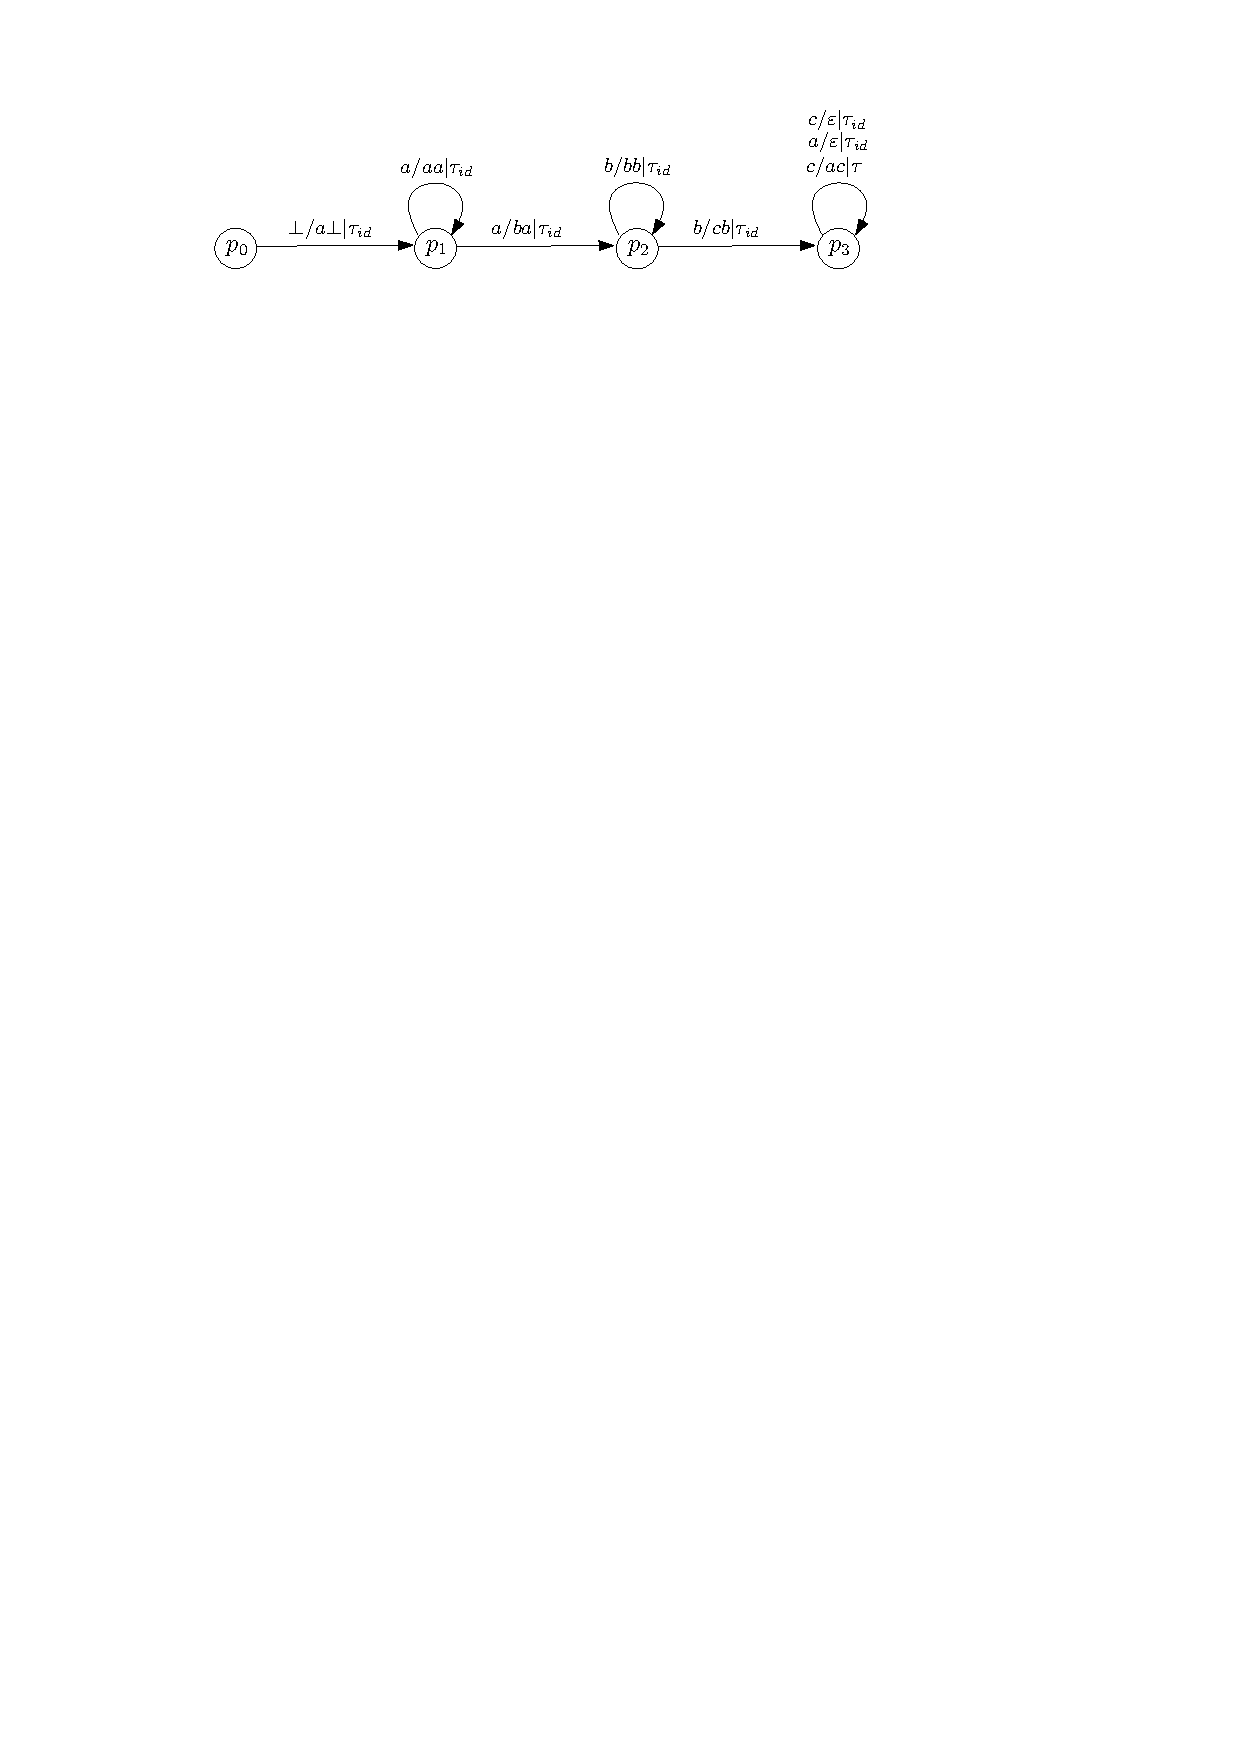
\includegraphics[scale = 0.9]{wstrpds-example.pdf}
	\caption{An example for \WOTrPDS}\label{fig-wstrpds-exmp}
\end{figure}

\begin{example}\label{exmp-wpotrpds}
Consider the {\WOTrPDS} $\Pp=(P, \Gamma, \TranSet, \Delta)$ (see Figure~\ref{fig-wstrpds-exmp}), where 
\begin{itemize}
\item $P = \{p_0, p_1, p_2, p_3\}$,  $\Gamma = \{\bot, a, b, c, d\}$,
% 
\item $\TranSet = \{\tau_{id}, \tau\}$, where $\tau$ is the transduction defined as follows: upon an input $w \in \Gamma^*$ where $a$ occurs at least once, it replaces at least the first occurrence of $a$ by $d$, more precisely, it nondeterministically chooses some $n \ge 1$ and replaces each of the first $n$ occurrences of $a$ in $w$ by $d$, for instance, $\tau(babad\bot) = \{bdbad\bot, bdbdd\bot\}$,
%
\item $\Delta$ is as illustrated in Figure~\ref{fig-wstrpds-exmp}, in particular, $(p_3, c, ac, \tau, p_3) \in \Delta$. 
%\left\{
%\begin{array}{l}
%(q_0, \bot, a\bot, \tau_{id}, q_1), (q_1, a, aa, \tau_{id}, q_1), (q_1, a, ba, \tau_{id}, q_2), (q_2, b, bb, \tau_{id}, q_2), \\
%(q_2, b, cb, \tau_{id}, q_3), (q_3, c, ac, \tau_1, q_3), (q_3, a, \epsilon, \tau_{id}, q_3) 
%\end{array}
%\right\}$.
\end{itemize}

From the definition of $\Delta$, $(p_3, bbdd\bot)$ is reachable from $(p_0, \bot)$, as witnessed by the following path in $\xrightarrow{\Pp}$, 
\[
\begin{array}{l}
(p_0, \bot) \xrightarrow{\Pp} (p_1, a \bot) \xrightarrow{\Pp} (p_1, aa \bot) \xrightarrow{\Pp} (p_2, baa \bot)  \xrightarrow{\Pp} (p_2, bbaa \bot)  \xrightarrow{\Pp} (p_3, cbbaa \bot)  \\
\xrightarrow{\Pp} (p_3, acbbdd \bot) \xrightarrow{\Pp} (p_3, cbbdd \bot)  \xrightarrow{\Pp} (p_3, bbdd \bot). 
\end{array}
\]
Note that, from the configuration $(p_3, cbbaa \bot)$, the transition $p_3 \xrightarrow{c/ac|\tau } p_3$ is applied. Then  $bbaa$ is transformed by $\tau$ into $bbdd$, moreover, $a$ is pushed. Therefore, the configuration $(p_3, acbbdd)$ is produced.

It is necessary to verify that $(\langle \TranSet \rangle, \preceq)$ has a well-partially-ordered union-basis $\Tranbasis$. First, we observe that $\tau^1 \supseteq \tau^2 \supseteq \cdots$, where $\tau^i$ for $i \ge 1$ is the $i$-fold composition of $\tau$, more specifically, $\tau^i$ nondeterministically replaces each of the first $n $ occurrences of $a$ in an input $w$ by $d$ for some $n \ge i$. It follows that $\tau^i \cup \tau^j = \tau^i$ for every $i < j$.
Moreover, $\lceil a, d \rfloor^{-1} \tau = \tau_{id} \cup \tau$. Therefore, the transduction closure $\langle \TranSet \rangle$ is $\{\emptyset, \tau_{id}, \tau_\varepsilon\} \cup \{\tau^i \mid i \ge 1\} \cup \{\tau_{\varepsilon} \cup \tau^i \mid i \ge 1\} \cup \{\tau_{id} \cup \tau^i \mid i \ge 1\}$. Let $\Tranbasis = \{\emptyset, \tau_{id}, \tau_\varepsilon\} \cup \{\tau^i \mid i \ge 1\}$. Then $\Tranbasis$ is a union-basis of $\langle \TranSet \rangle$. 
%, where $\tau^i$ is the $i$-fold composition of $\tau$, more specifically, $\tau^i$ nondeterministically replaces each of the first $n $ occurrences of $a$ in $w$ by $d$ for some $n \ge i$. 
%Note that $\tau_i$ is obtained as the $i$-fold composition of $\tau$. 
%
From $\tau^1 \supseteq \tau^2 \supseteq \cdots$, we deduce that each infinite descending chain of $(\Tranbasis, \preceq)$, i.e. each infinite ascending chain of $(\Tranbasis, \subseteq)$, eventually stabilizes at $\emptyset, \tau_{id}, \tau_\varepsilon$, or $\tau^i$ for some $i$. Thus $(\Tranbasis, \preceq)$ contains no infinite strictly descending chains, i.e. it satisfies the DCC condition. Moreover, from $\tau^1 \supseteq \tau^2 \supseteq \cdots$, we know that it contains no infinite antichains as well. We conclude that $(\Tranbasis, \preceq)$ is a wpo. The distributivity of $\preceq$ over $\Tranbasis$-representations is evident. \qed
%
%An example of {\WSTrPDS} here.
\end{example}

\begin{theorem}\label{thm-wstrpds-wpo}
	Given a {\WOTrPDS} $\Pp = (P, \Gamma, \TranSet, \Delta)$, and $\Tranbasis$ is the union-basis of $\langle \TranSet \rangle$, then $\overline{\Tranbasis}$ is the union-basis of $\langle \overline{\TranSet}\rangle$.
\end{theorem}
We prove Theorem~\ref{thm-wstrpds-wpo} by showing $\overline{\Tranbasis}$ satisfied the four conditions in Definition~\ref{def:defatpds}.
\begin{proof}
	First, by the definition of $\overline{\Tranbasis}$, we have that $\{\emptyset, \tau_{\epsilon}\}\subseteq \overline{\Tranbasis}$.

	Now we prove $(\overline{\Tranbasis}, \preceq)$ is a wpo. By the definition of $\overline{\Tranbasis}$, for every $\overline{\beta_1},\overline{\beta_2}\in\overline{\Tranbasis}$, if $\overline{\beta_1}\neq\emptyset$ and $\overline{\beta_2}\neq \emptyset$, then $\overline{\beta_1}\preceq\overline{\beta_2}$ iff $\beta_1\preceq\beta_2$. Since $(\Tranbasis, \preceq)$ is a wpo, we deduce that $(\overline{\Tranbasis}, \preceq)$ is a wpo.

	Then we prove for each $\overline{\tau}\in\langle\overline{\TranSet}\rangle$, a $\overline{\Tranbasis}$-representation $\beta_{\overline{\tau}}$ can be computed effectively.
	Since $\langle\overline{\TranSet}\rangle = \overline{\langle \TranSet \rangle}$, then for each $\overline{\tau}\in\langle\overline{\TranSet}\rangle$, we have $\tau \in \langle \TranSet \rangle$. 
	Suppose that $\tau$ can be rewritten into the $\Tranbasis$-representation $\beta_1\cup\cdots\cup\beta_m$, then it is easy to observe that $\overline{\tau} = \overline{\beta_1}\cup\cdots\cup\overline{\beta_m}$, where $\overline{\beta_1},\cdots,\overline{\beta_m} \in \overline{\Tranbasis}$. Therefore $\overline{\beta_1}\cup\cdots\cup\overline{\beta_m}$ is the $\overline{\Tranbasis}$-representation of $\overline{\tau}$.

	Finally, we prove $\preceq$ is union-distributive over $\overline{\Tranbasis}$-representations, specifically, for each $\overline{\beta} \in \overline{\Tranbasis}$ and $\overline{\tau} \in \langle \overline{\TranSet} \rangle$ whose $\overline{\Tranbasis}$-representation is $\beta_{\overline{\tau}}=\beta_{\overline{\tau}, 1} \cup \cdots \cup \beta_{\overline{\tau}, n_{\overline{\tau}}}$, if $\overline{\tau} \preceq \overline{\beta}$, then $ \beta_{\overline{\tau}, i} \preceq \overline{\beta}$ for some $i \in [n_{\overline{\tau}}]$.

	For each $\overline{\beta} \in \overline{\Tranbasis}$ and $\overline{\tau} \in \langle \overline{\TranSet} \rangle$ whose $\overline{\Tranbasis}$-representation is $\beta_{\overline{\tau}}=\beta_{\overline{\tau}, 1} \cup \cdots \cup \beta_{\overline{\tau}, n_{\overline{\tau}}}$, we have that $\beta\in\Tranbasis$ and $\tau = \beta_{\tau,1}\cup \cdots \cup \beta_{\tau,n_\tau} \in \TranSet$, where $n_\tau = n_{\overline{\tau}}$ and for each $i\in[n_\tau]$, $\beta_{\overline{\tau}, i} = \overline{\beta_{\tau, i}}$.
	Then if $\overline{\tau}\preceq\overline{\beta}$, we have $\tau \preceq \beta$, i.e., $\beta\subseteq \tau$. Since $\Tranbasis$ is the union-basis of $\langle \TranSet \rangle$, we have $\beta_{\tau, i}\preceq \beta$, i.e., $\beta\subseteq\beta_{\tau, i}$ for some $i\in[n_\tau]$. Then we have $\overline{\beta}\subseteq \beta_{\overline{\tau}, i}$, i.e., $\beta_{\overline{\tau}, i} \preceq \overline{\beta}$.
	\qed

\end{proof}

In this paper, we consider the \emph{regular reachability problem} of {\WOTrPDS}.
\begin{quote} 
	Given a {\WOTrPDS} $\Pp = (P, \Gamma, \TranSet, \Delta)$, control states $p_1, p_2 \in P$, regular languages $L_1, L_2$ over $\Gamma$, determine whether there exist %strings $w_1, w_2$ such that 
	$w_1 \in L_1$, $w_2 \in L_2$ such that $(p_1, w_1) \xRightarrow{\Pp} (p_2, w_2)$.
\end{quote}
%\begin{itemize}
%\item The \emph{reachability problem} is to check for two given configurations $(q_1, w_1)$ and $(q_2, w_2)$, whether $(q_1, w_1) \xRightarrow{\Pp} (q_2, w_2)$.
%
%\item 
%\end{itemize}

%We will show that the regular reachability problem of {\WOTrPDS} is decidable. In the next section, a model called finite automata with well-ordered transductions will be introduced, to represent sets of configurations of {\WOTrPDS}.


\begin{theorem}\label{thm-wstrpds-reach}
The regular reachability problem of {\WOTrPDS} is decidable.
\end{theorem}

Fix a  {\WOTrPDS} $\Pp = (P, \Gamma, \TranSet, \Delta)$. %and $\Aut = (Q, \Gamma, \delta, P, F)$ be a $\Pp$-{\NFA}. 
We show Theorem~\ref{thm-wstrpds-reach} via the saturation technique, which %by applying the saturation procedures from \cite{SM+15,Song18}. 
requires to represent the set of reachable configurations of $\Pp$. For traditional pushdown systems, a tailored {\NFA} (commonly referred to as P-automata in literature) suffices. For {\WOTrPDS}, we %generalize P-automata to 
introduce a new model, viz., \emph{finite automata with well-partially-ordered transductions} ({\WOTrNFA}), in Section~\ref{sec-wotrnfa}. 
Then in Section~\ref{sect:decidability}, we utilize the saturation technique to reduce the regular reachability problem of {\WOTrPDS} %the decidability % by reducing 
to the intersection problem of {\WOTrNFA} and {\NFA}, which is shown to be decidable in Section~\ref{sec:fatrnfa}.

We prove Theorem~\ref{thm:st-amass-reach} by showing that a {\WOTrPDS} $\Pp_\Mm = (P_\Mm, \Gamma_\Mm, \TranSet_\Mm, \Delta_\Mm)$ can be constructed from a given {\AMASS} $\Mm = (\act, A_0,\lmd,\aft,\Delta)$ to simulate the behaviors of $\Mm$. We show the details in Section~\ref{sec-proof-reach}


\subsection{Finite automata with well-partially-ordered transductions}\label{sec-wotrnfa}
 
\begin{definition}[Finite automata with well-partially-ordered transductions, {\WOTrNFA}] %[Finite automata with finite ascending chians and antichains transductions]
	Given a {\WOTrPDS} $\Pp=(P, \Gamma, \TranSet, \Delta)$ with $\Tranbasis$ as the union-basis of $\langle \TranSet \rangle$, a $\Pp$-{\WOTrNFA} is a tuple $\Aut =(Q, \Gamma, \delta, I, 
	F)$,
	where $Q$ is the set of states such that $P \subseteq Q$, $I\subseteq P\subseteq Q$ is the set of initial states, $F$ is the set of final states,  
	%and the set of initial states is $P$, %is a finite set of states, $\Sigma$ is a finite alphabet, 
	%$\TranSet$ is a finite set of transductions, %$I \subseteq Q$ (reps. $F \subseteq Q$) is a finite set of initial (reps. final) states, 
	and $\delta \subseteq Q \times \Gamma_\varepsilon \times \Tranbasis \times Q$ is a finite set of transition rules.

    A $\Pp$-{\WOTrNFA} $\Aut$ is called a {$\Pp$-{\NFA}} if for every $(q, a, \beta, q')$, $\beta = \tau_{id}$. 
\end{definition}

For convenience, we write a transition $(q, a, \beta, q')$ as $q \xrightarrow{a | \beta} q'$. 
To define the semantics of $\Aut$, we extend the transition rules $q \xrightarrow{a | \beta} q' \in \delta$  to a relation $q \xRightarrow{w | \tau} q'$ for a string $w$,  
%
%The relation $q \xRightarrow{w | \tau} q'$ is  
defined inductively as follows:
\begin{itemize}
	\item if $q \xrightarrow{a |\beta} q'$, then $q \xRightarrow{a | \beta} q'$, 
	%
	\item if $q \xRightarrow{w | \tau} q'$ and $q' \xrightarrow{b |\beta } q'' $, then $q \xRightarrow{w a | (\lceil a, b\rfloor^{-1}\tau) \circ \beta} q''$ for every $a \in \Gamma_\varepsilon$ such that $\lceil a, b\rfloor^{-1}\tau \neq \emptyset$.
\end{itemize}
Intuitively, $q \xRightarrow{w | \tau} q'$ means that in $\Aut$,  $q'$ is reached starting from $q$ after reading $w$. Moreover, the transduction $\tau$, which is  to be applied to the remaining suffix of the input string, is produced. Note that the transduction  $\tau \in \langle \TranSet \rangle$ in $q \xRightarrow{w | \tau} q'$ may not be in $\Tranbasis$. 

A configuration $(p, w)$ of $\Pp$ is accepted by $\Aut$ if $p\in I$ and $p \xRightarrow{w | \tau} q$ for some $q \in F$ and $\tau \in \langle \TranSet \rangle$ such that $(\varepsilon, \varepsilon) \in \tau$.
%
Let us use $\confs(\Aut)$ to denote the set of configurations of $\Pp$ accepted by $\Aut$.
Moreover, let $\ConfSet(\Aut)$ to denote the set of words $w$ such that $(p, w)\in\confs(\Aut)$ for some $p \in I$.
For a $\Pp$-$\WOTrNFA$ $\Aut = (Q, \Gamma, \delta, I, F)$, we use $\Aut(p')$ to denote to denote the $\Pp$-$\WOTrNFA$ obtained from $\Aut$ by replacing $I$ with $\{p'\}$.

It turns out that $\Pp$-{\WOTrNFA} is capable of representing \emph{non-regular} set of configurations, as %witnessed 
shown by the following example.
\begin{example}
Let $\Pp$ be the {\WOTrPDS} in Example~\ref{exmp-wpotrpds}. Consider the $\Pp$-{\WOTrNFA} $\Aut = (Q, \Gamma, \delta, I, F)$ in Figure~\ref{fig-ptrnfa-exmp}, where $F= \{q_1\}$ and $\tau$ is the transduction from $\Pp$ that replaces at least the first occurrence of $a$ by $d$. From $p_3 \xrightarrow{c | \tau} p_3$, $p_3 \xrightarrow{b | \tau_{id}} q_1$, we have $p_3  \xRightarrow{c b | (\lceil b, b\rfloor^{-1} \tau) \circ \tau_{id}} q_1$, thus $p_3 \xRightarrow{cb | \tau} q_1$. Moreover, from $q_1 \xrightarrow{d | \tau_{id}} q_1$, we deduce $p_3 \xRightarrow{c b a | (\lceil a, d\rfloor^{-1} \tau) \circ \tau_{id}} q_1$. Since $(\lceil a, d\rfloor^{-1} \tau) \circ \tau_{id} = \tau_{id} \cup \tau$, we have $p_3 \xRightarrow{c b a |  \tau_{id} \cup \tau} q_1$ and $(\epsilon, \epsilon) \in \tau_{id} \cup \tau$. Thus $(p_3, cba)$ is accepted by $\Aut$. On the other hand, although $p_3 \xRightarrow{cb | \tau} q_1$ with $q_1 \in F$, but $(\epsilon, \epsilon) \not \in \tau$, thus $(p_3, cb)$ is not accepted by $\Aut$.  Furthermore, we observe that for $m \ge 1$, $p_3 \xRightarrow{c^m | \tau^m} p_3$. From the fact that $\tau^m$ replaces at least $m$ occurrences of $a$ by $d$, we deduce that for each configuration of the form $(p_3, c^m b a^n)$ with $m,n \ge 1$, it is accepted by $\Aut$ iff $n \ge m$.  Therefore, $\confs(\Aut)$, the set of configurations accepted by $\Aut$, is non-regular. 
%
\begin{figure}[htb]
    \centering
	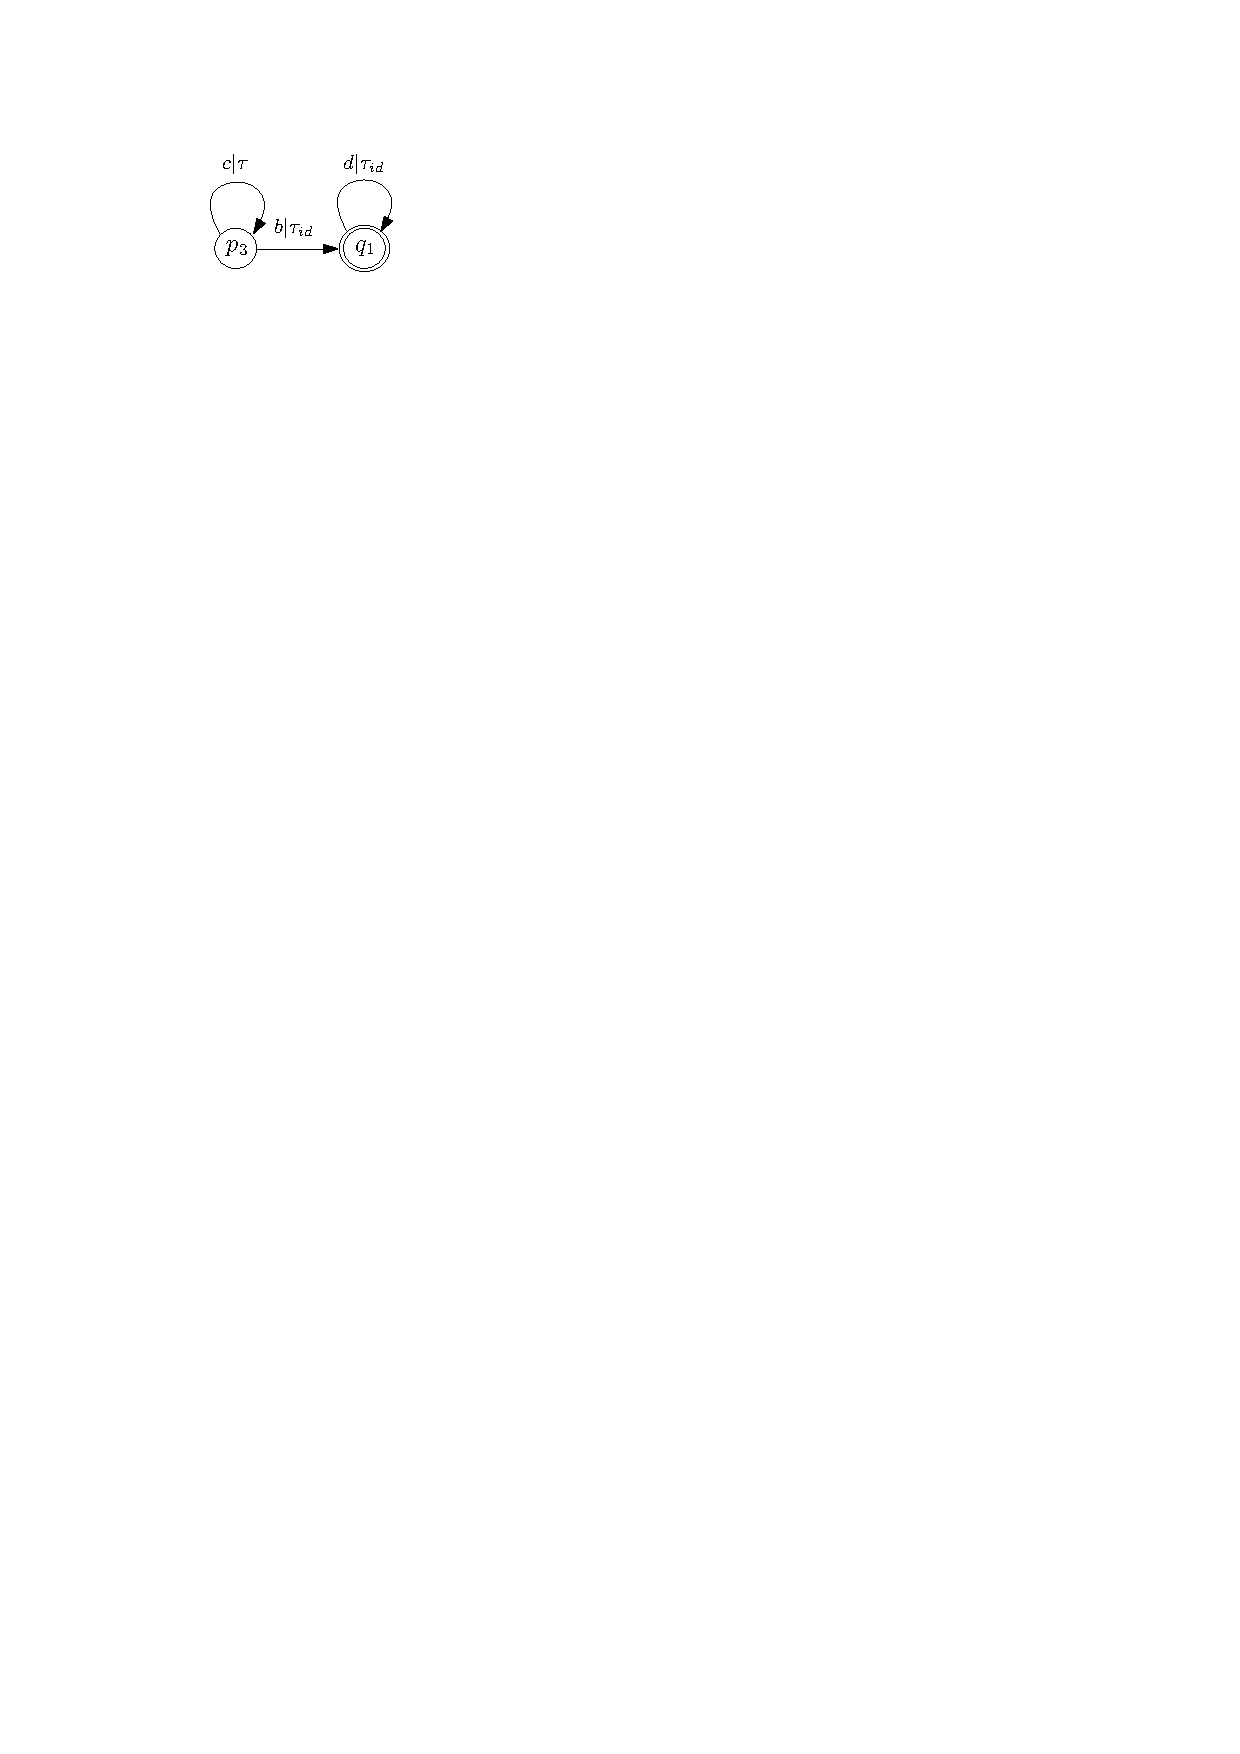
\includegraphics[scale = 0.9]{pwpotrnfa-example.pdf}
	\caption{An example of $\Pp$-\WOTrNFA}\label{fig-ptrnfa-exmp}
\end{figure}
\qed
\end{example}

For a $\Pp$-{\WOTrNFA} $\Aut$, $\pre^*_\Pp(\confs(\Aut))$  denotes the set of configurations $(p, w)$ of $\Pp$ such that $(p, w) \xRightarrow{\Pp} (p', w')$ for some $(p', w') \in \confs(\Aut)$. Accordingly, $\post^*_\Pp(\confs(\Aut))$ denotes the set of configurations $(p, w)$ of $\Pp$ such that $(p', w') \xRightarrow{\Pp} (p, w)$ for some $(p', w') \in \confs(\Aut)$.





%%%%%%%%%%%%%%%%%%%%%%%%%%%%%%%%%%%%%%%%%%%%%%%%%
%%%%%%%%%%%%%%%%%%%%%%%%%%%%%%%%%%%%%%%%%%%%%%%%%
\subsection{Saturation} \label{sect:decidability}
Let $\Pp = (P, \Gamma, \TranSet, \Delta)$ be a  {\WOTrPDS} where $\Tranbasis$, the union-basis of  $\langle \TranSet \rangle$, is a wpo, and let $\Aut = (Q, \Gamma, \delta, I, F)$ be a $\Pp$-{\WOTrNFA}. %We prove Theorem~\ref{thm-wstrpds-reach} by 
We apply the saturation procedures from \cite{SM+15,Song18} to obtain a $\Pp$-{\WOTrNFA} $\Aut^{\pre^*}_{\Pp}$ (resp. $\Pp$-{\WOTrNFA} $\Aut^{\post^*}_{\Pp}$), which represents $\pre^*_\Pp(\confs(\Aut))$ (resp. $\post^*_\Pp(\confs(\Aut))$).

% Let $\Pp = (P, \Gamma, \TranSet, \Delta)$ be a  {\WOTrPDS} where $\Tranbasis$, the union-basis of  $\langle \TranSet \rangle$, is a wpo, and let $\Aut = (Q, \Gamma, \delta, F)$ be a $\Pp$-{\NFA}. %We prove Theorem~\ref{thm-wstrpds-reach} by 
% We apply the saturation procedures from \cite{SM+15,Song18} to obtain a $\Pp$-{\WOTrNFA} $\Aut^{pre^*}$, which represents $pre^*_\Pp(\ConfSet(\Aut))$ and 
%represents the set of configurations reachable from the initial configuration. 
%The termination of the saturation procedures is guaranteed by the assumption that the transduction closure is well-ordered.  Then the regular reachability problem is reduced to the {\WOTrNFA}-{\NFA} intersection problem for $\Aut$ and $\AutB$, which is decidable according to Proposition~\ref{prop-wstrnfa-nfa-intersect}.
%
%In the sequel, we first recall the two saturation procedure in \cite{SM+15,Song18}, then prove its termination.
%
%Let $\Aut = (Q', \Gamma, \delta', P, F')$ be a $\Pp$-{\WOTrNFA} such that for each pair of states $(q_1, q_2)$ and each $\gamma \in \Gamma_\varepsilon$, there is at most one $\tau'' \in \langle \TranSet \rangle$ satisying that $(q_1, \gamma, \tau'', q_2) \in \delta'$. 
%
%The $\Pp$-{\WOTrNFA} $\Aut^{pre^*}$ 
\paragraph{Computing $\pre^*$}
$\Aut^{\pre^*}_{\Pp}$ is constructed by iteratively adding the transitions to $\Aut$, according to the following saturation rule. 
%$\Aa^{pre^*} $ is obtained from $\Aa$ by adding the transitions according to the following three saturation rules.

\smallskip

\fbox{
%
\begin{minipage}{0.9\textwidth}
%\begin{enumerate}
    Let $\Aut'$ be the current $\Pp$-{\WOTrNFA}.
     For $(p_1, \gamma, w, \tau, p_2) \in \Delta$ and $p_2  \xRightarrow{w\mid\tau'} q'$ in $\Aut'$, suppose that a $\Tranbasis$-representation of $\tau\circ\tau'$ is $\beta_1 \cup \cdots \cup \beta_n$ where $\beta_i \in \Tranbasis$ for each $i \in [n]$,  %we do the following: 
%     Suppose that a $\Tranbasis$-representation of $\tau\circ\tau'$ is $\beta_1 \cup \cdots \cup \beta_n$ where $\beta_i \in \Tranbasis$ for each $i \in [n]$.
     %
     for each $i \in [n]$ such that there does \emph{not} exist a transition $(p_1, \gamma, \tau'', q')$ in $\Aut'$ with $\tau'' \preceq \beta_i$ (i.e. $\tau'' \supseteq \beta_i$),  we update $\Aut'$ by adding a transition $(p_1, \gamma, \beta_i, q')$.
     %
%     if there is a transition $(p_1, \gamma, \tau'', q')$ in the current $\Pp$-{\WOTrNFA}, then we replace $(p_1, \gamma, \tau'', q')$ with the transition $(p_1, \gamma, (\tau\circ\tau') \cup \tau'', q')$, otherwise, we add a transition $(p_1, \gamma,\tau\circ\tau', q')$.
%\end{enumerate}
\end{minipage}
}
\smallskip

\paragraph{Computing $\post^*$}
$\Aut^{\post^*}_{\Pp}$ is constructed by iteratively adding the transitions to $\Aut$, according to the following saturation rule. 
%$\Aa^{pre^*} $ is obtained from $\Aa$ by adding the transitions according to the following three saturation rules.

\smallskip

\fbox{

\begin{minipage}{0.9\textwidth}
    Let $\Aut'$ be the current $\Pp$-{\WOTrNFA}. For $(p_1, \gamma, w, \tau, p_2) \in \Delta$, and $p_1  \xRightarrow{\gamma\mid\tau'} q'$ in $\Aut'$, 
    suppose that a $\Tranbasis$-representation of $\overline{\tau}\circ\tau'$ is $\beta_1 \cup \cdots \cup \beta_n$ where $\beta_i \in \Tranbasis$ for each $i \in [n]$, 
    \begin{enumerate}
        \item if $w = \epsilon$ or $w=\gamma_1$, for each $i \in [n]$ such that there does \emph{not} exist a transition $(p_2, w, \tau'', q')$ in $\Aut'$ with $\tau'' \preceq \beta_i$ (i.e. $\tau'' \supseteq \beta_i$),  we update $\Aut'$ by adding a transition $(p_2, w, \beta_i, q')$.
        \item if $w = \gamma_1\gamma_2$, 
            \begin{itemize}
                \item suppose that a $\Tranbasis$-representation of $\tau_{\id}$ is $\beta_1' \cup \cdots \cup \beta_m'$ where $\beta_i' \in \Tranbasis$ for each $i \in [m]$, then for each $i\in[m]$, we update $\Aut'$ by adding a transition $(p_2,\gamma_1,\beta_i',\langle p_2,\gamma_1\rangle)$,
                \item for each $i \in [n]$ such that there does \emph{not} exist a transition $(\langle p_2,\gamma_1\rangle, \gamma_2, \tau'', q')$ in $\Aut'$ with $\tau'' \preceq \beta_i$ (i.e. $\tau'' \supseteq \beta_i$), we update $\Aut'$ by adding a transition $(\langle p_2,\gamma_1\rangle, \gamma_2, \beta_i, q')$.
            \end{itemize}

    \end{enumerate}
\end{minipage}
}
\smallskip
%Note that the aforementioned saturation rule guarantees the following property is preserved in the construction: For each pair of states $(q_1, q_2)$ and each $\gamma \in \Gamma_\varepsilon$, there is at most one $\tau'' \in \langle \TranSet \rangle$ satisying that $(q_1, \gamma, \tau'', q_2) \in \delta'$.


We now show that the saturation procedure for computing $\Aut^{\pre^*}_{\Pp}$ terminates. 
%The proof for computing $\Aut^{pre^*}$ is similar.
%
Towards contradiction, suppose that 
%the saturation procedure for computing $\Aut^{pre^*}$ 
it does not terminate. From the construction of $\Aut^{\pre^*}_{\Pp}$, there must be $q_1, q_2 \in Q'$, $\gamma \in \Gamma_\varepsilon$, and an infinite sequence of transductions $\beta_1, \beta_2, \cdots \in \Tranbasis$ such that the transitions $(q_1, \gamma, \beta_1, q_2) $, $(q_1, \gamma, \beta_2, q_2) $, $\cdots$ are added one by one,  and for every $i > 1$ and $j \le i$, $\beta_j \not \preceq \beta_i$,  that is, either $\beta_j$ and $\beta_i$ are incomparable or $\beta_j \succ \beta_i$. From infinite Ramsey theorem (cf. Theorem 9.1.2 in \cite{Rein00}), there must be an infinite sequence $i_1 < i_2 < \cdots$ such that $\beta_{i_1}, \beta_{i_2}, \cdots$ is either an infinite antichain or an infinite strictly descending chain. This contradicts the assumption that $(\Tranbasis, \preceq)$ is a wpo. 
The proof for computing $\Aut^{\post^*}_{\Pp}$ is similar.
%$\tau_1 \subset \tau_2 \subset \cdots$, that is, $\tau_1, \tau_2, \cdots$ is a strictly ascending chain with respect to $\subseteq$, thus a strictly descending chain with respect to $\preceq$. This contradicts the assumption that $(\langle \TranSet\rangle, \preceq) $ is a wpo.


\begin{example}
Let us continue Example~\ref{exmp-wpotrpds}. Let $\Aut = (Q, \Gamma, \delta, I, F)$ be the $\Pp$-{\WOTrNFA} recognizing the configurations $\{(p_3, b^m d^n \bot) \mid m > 0, n > 0\}$ (see Figure~\ref{fig-pnfa-exmp}). More specifically, $Q= P \cup \{q_1, q_2, q_3\}$, $I = \{p_3\}$, $F= \{q_3\}$, and $\delta$ is illustrated by the edges in Figure~\ref{fig-pnfa-exmp} (where the identity transduction $\tau_{id}$ in the transitions is omitted).  
%More specifically, $Q = \{p_3, q_1, q_2\}$
%
\begin{figure}[htb]
    \centering
	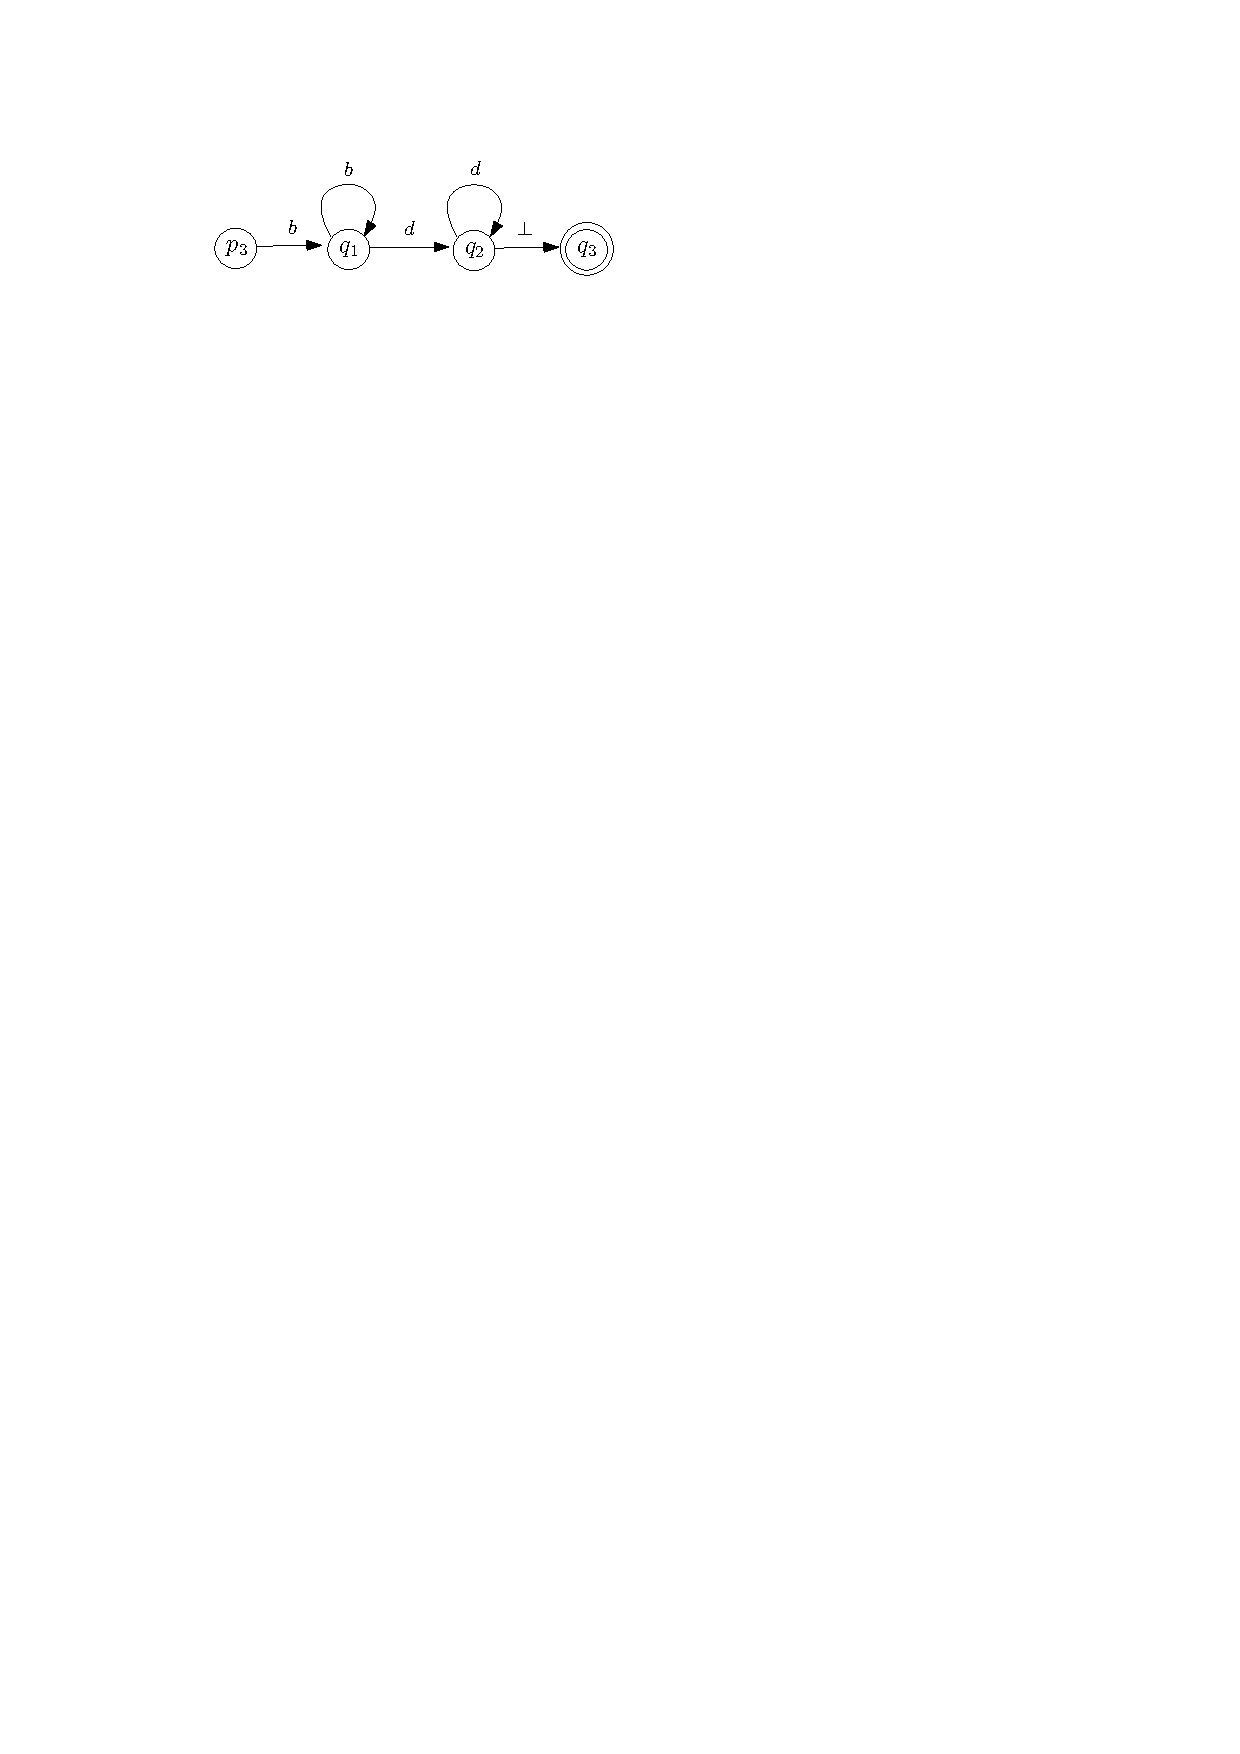
\includegraphics[scale = 0.9]{pnfa-example.pdf}
	\caption{An example of $\Pp$-{\WOTrNFA} $\Aut$}\label{fig-pnfa-exmp}
\end{figure}

Then we apply the saturation rule to add transitions.
\begin{itemize}
\item In the beginning, because $(p_3, a, \varepsilon, \tau_{id}, p_3) \in \Delta$ and $p_3 \xRightarrow{\varepsilon | \tau_{id}} p_3$ in $\Aut$, the transition $(p_3, a, \tau_{id}, p_3)$ is added according to the saturation rule. Similarly, the transition $(p_3, c, \tau_{id}, p_3)$ is added. 
%
\item Because $(p_3, c, ac, \tau, p_3) \in \Delta$, $p_3 \xRightarrow{ac | \tau_{id}} p_3$  in the current $\Pp$-{\WOTrNFA}, $\tau \circ \tau_{id} = \tau \in \Tranbasis$, and 
 there already exists a transition $(p_3, c, \tau_{id}, p_3)$, moreover, $\tau_{id} \not \preceq \tau$, the transition $(p_3, c, \tau, p_3)$ is added according to the saturation rule. 
%
\item Similarly, since $(p_2, b, cb, \tau_{id}, p_3) \in \Delta$, $p_3 \xRightarrow{cb | \tau_{id}} q_1$ and $p_3 \xRightarrow{cb | \tau} q_1$ in the current $\Pp$-{\WOTrNFA}, two transitions $(p_2, b, \tau_{id}, q_1)$  and $(p_2, b, \tau, q_1)$ are added. 
%
\item Furthermore, because $(p_1, a, ba, \tau_{id}, p_2) \in \Delta$ and $p_2 \xRightarrow{ba | \tau_{id} \cup \tau} q_2$ in the current $\Pp$-{\WOTrNFA} (This follows from $p_2 \xrightarrow{b | \tau} q_1$, $q_1 \xrightarrow{d | \tau_{id}} q_2$, and $(\lceil a, d\rfloor^{-1} \tau) \circ \tau_{id} = \tau_{id} \cup \tau$.), two transitions $(p_1, a, \tau_{id}, q_2)$  and $(p_1, a, \tau, q_2)$ are added.
%
%\item Furthermore, because $(p_2, b, cb, \tau_{id}, p_3) \in \Delta$, $p_3 \xRightarrow{cb | \tau} q_1$ in the current $\Pp$-{\WOTrNFA}, $ \tau_{id} \circ \tau = \tau \in \Tranbasis$, and there already exists a transition $(p_2, b, \tau_{id}, q_1)$, moreover, $\tau_{id} \not \preceq \tau$,
%the transition $(p_2, b, \tau, q_1)$ is added. 
\end{itemize}
By iterating this process, in the end, we obtain $\Aut^{\pre*}_{\Pp}$, as illustrated in Figure~\ref{fig-saturation-exmp}.
\begin{figure}[htb]
    \centering
	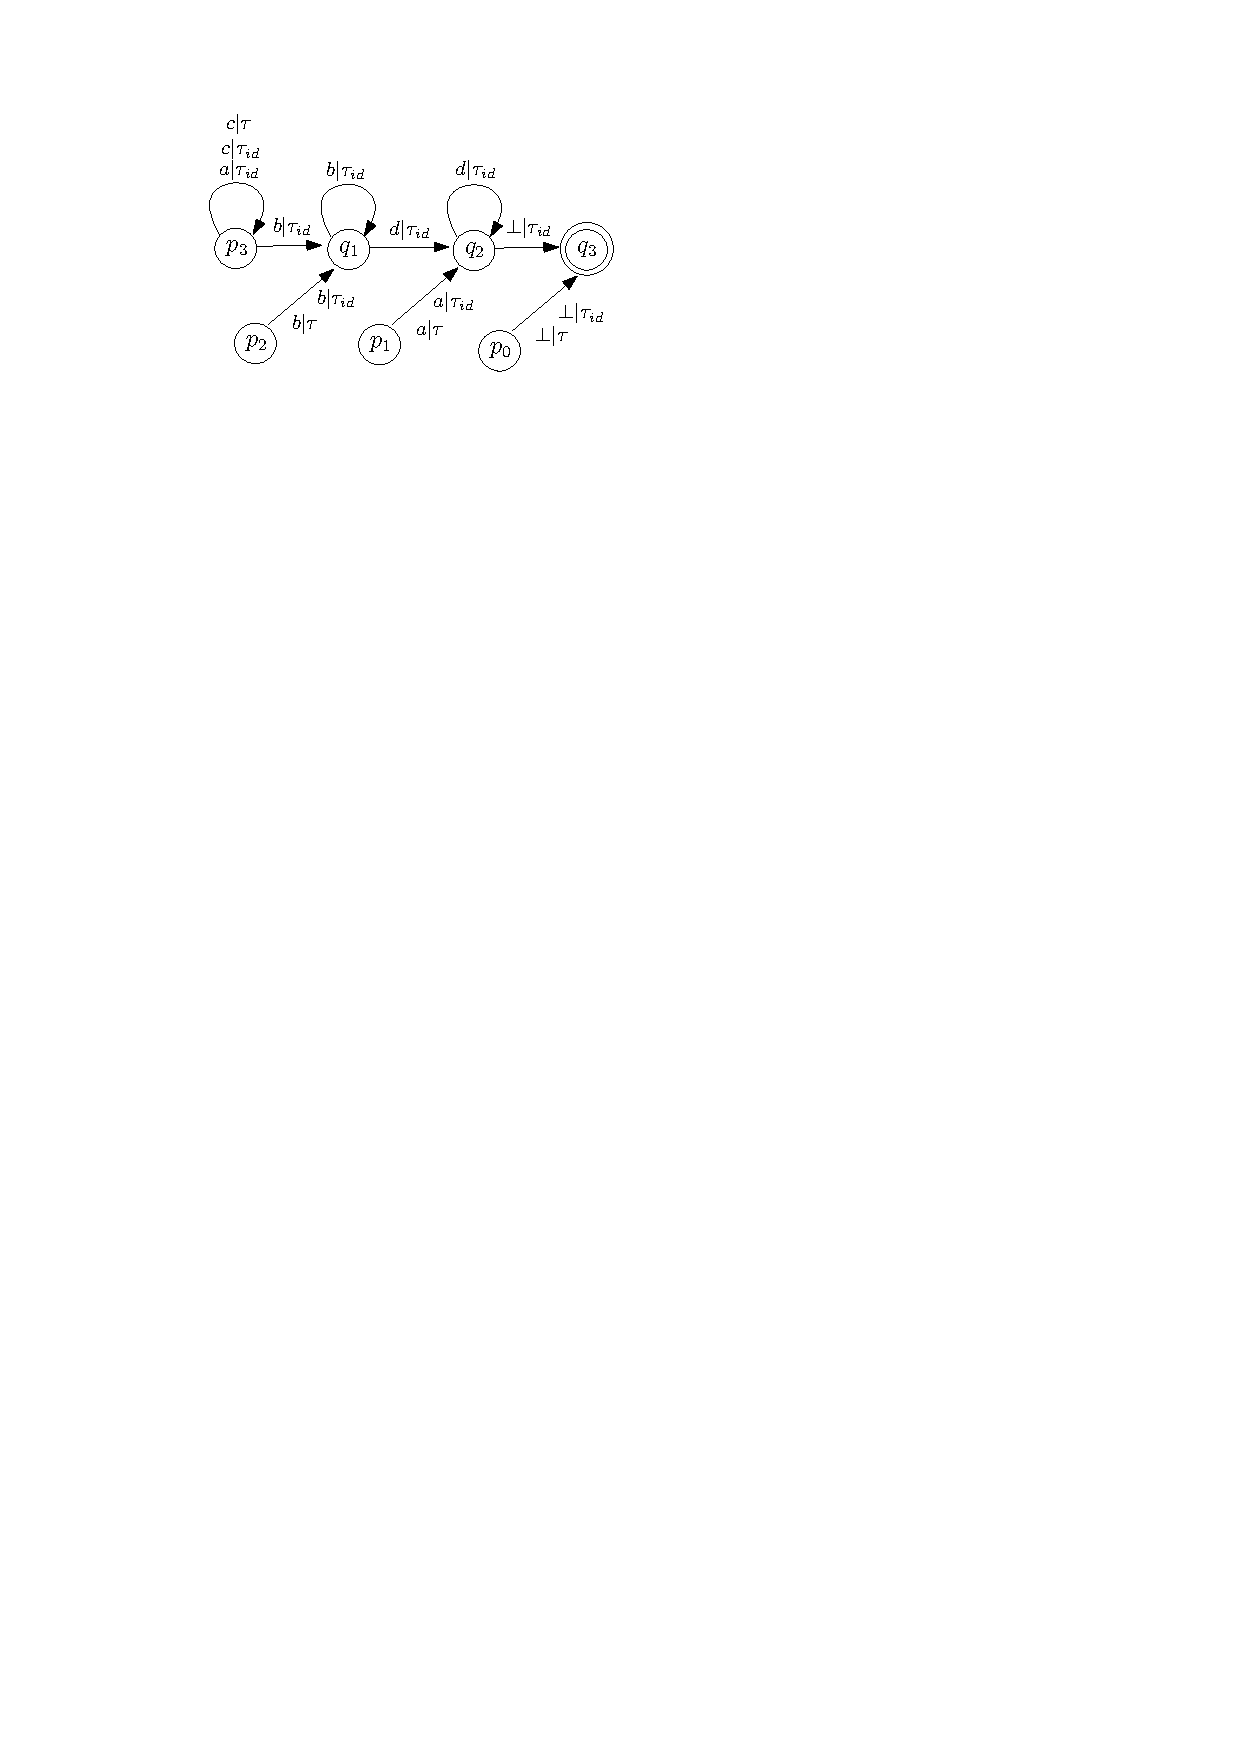
\includegraphics[scale = 0.9]{saturation-example.pdf}
	\caption{The $\Pp$-{\WOTrNFA} $\Aut^{\pre*}_{\Pp}$}\label{fig-saturation-exmp}
\end{figure}
\qed
\end{example}

Given the {\WOTrPDS} $\Pp= (P, \Gamma, \TranSet, \Delta)$, $p_1, p_2 \in P$, and two regular languages $L_1, L_2$ represented by {\NFA}s $\Aut_1 = (Q_1, \Gamma, \delta_1, I_1, F_1)$ and $\Aut_2 = (Q_2, \Gamma, \delta_2, I_2, F_2)$ respectively, the regular reachability problem is reduced to the intersection problem of the $\Pp$-{\WOTrNFA} $(\Aut_1'(p_1))^{\post*}_{\Pp}$ and the $\Pp$-{\NFA} $\Aut_2(p_2)$, 
i.e., checking $\ConfSet((\Aut_1'(p_1))^{\post*}_{\Pp}) \cap \ConfSet(\Aut_2(p_2)) \neq \emptyset$, where $\Aut_1' = (Q_1, \Gamma, \delta_1', I_1, F_1)$ and $\delta_1' = \{(p,\gamma,\tau_{\id}, p')\mid (p,\gamma,p')\in\delta_1\}$.
% where $\Aut_1[p_1]$ is obtained from $\Aut_1$ by adding a transition $(p_1, a, q)$ for each $(q_0, a, q) \in \delta_1$ with $q_0 \in I_1$, similarly for $\Aut_2[p_2]$. 
Then Theorem~\ref{thm-wstrpds-reach} follows from Proposition~\ref{prop-wstrnfa-nfa-intersect} in the next subsection.

%Here when we add a transition $(p,\gamma,\tau'',p')$ into $\Aa$, if there exists a transition $(p, \gamma,\tau',p')$ in the current automaton, we modify the transition $(p,\gamma,\tau',p')$ to $(p,\gamma,\tau'\cup\tau'',p')$ instead of adding $(p,\gamma,\tau'',p')$.


\subsection{The intersection problem of {\WOTrNFA} and {\NFA}} \label{sec:fatrnfa}
%\begin{definition}[{\WOTrNFA}-{\NFA} intersection problem]
The {\WOTrNFA}-{\NFA} intersection problem is, for given $\Pp$-{\WOTrNFA} $\Aut$ and $\Pp$-{\NFA} $\AutB$, to decide  whether $\ConfSet(\Aut) \cap \ConfSet(\AutB) = \emptyset$. We shall show that this problem %the {\WOTrNFA}-{\NFA} intersection problem to 
can be reduced to (polynomially many) instances of the sub-covering problem of a downward-WSTS, which is decidable by Theorem~\ref{thm-dwsts}.
%\end{definition}

%The rest of this section is devoted to the proof of the following result.
\begin{proposition}\label{prop-wstrnfa-nfa-intersect}
	The {\WOTrNFA}-{\NFA} intersection problem is decidable.
\end{proposition}

%For technical convenience, we define another partial order $\preceq$ on $\langle \TranSet \rangle$ as follows: $\tau_1 \preceq \tau_2$ if $\tau_1 \supseteq \tau_2$. Moreover, we use $\tau_1 \prec \tau_2$ to denote $\tau_1 \supset \tau_2$ (i.e. $\tau_1 \supseteq \tau_2$ but $\tau_1 \neq \tau_2$).

%From the fact that $(\langle \TranSet \rangle, \subseteq)$ is dually well-ordered, namely, it satisfies the ACC condition and contains no infinite antichain, we deduce that $(\langle \TranSet \rangle, \preceq)$ is well-ordered, namely, it satisfies the DCC condition and contains no infinite antichain.

%$(\langle \TranSet \rangle, \preceq)$ is well-ordered


%In the sequel, we are going to prove Proposition~\ref{prop-wstrnfa-nfa-intersect} by reducing 

%Its proof relies on the decidability of the sub-covering problem of downward-WSTS (\cite{FS01}).
% $(T, \rightarrow, \preceq)$.

\begin{proof}
%Let us fix a {\WOTrPDS} $\Pp = (P, \Gamma, \TranSet, \Delta)$, 
Assume a $\Pp$-{\WOTrNFA} $\Aut = (Q, \Gamma, \delta, I, F)$ and a $\Pp$-{\NFA} $\AutB = (Q', \Gamma, \delta', I', F')$.
We construct a downward-WSTS $\wstsnodes_{\Aut,\AutB} = (S, \rightarrow, \preceq)$ 
%
%The basic idea of $\wstsnodes_{\Aut,\AutB}$ is 
to simulate the synchronized runs of $\Aut$ and $\AutB$, where
\begin{itemize}
	\item $S = Q \times \Tranbasis \times Q'$, (Intuitively, $(q, \beta, q') \in S$ means that the current states of $\Aut$ and $\AutB$ are $q$ and $q'$ respectively, and $\beta$ is the transduction to be applied to the remaining suffix of the input string.)
	%
	\item the transition relation $\xrightarrow{}$ is defined as follows:  for every state $(q_1, \beta_1, q'_1)$ in $S$ and transition rules $(q_1, b, \beta, q_2) \in \delta$ and $(q'_1, a, q'_2) \in \delta'$, suppose that a $\Tranbasis$-representation of $( \lceil a, b \rfloor^{-1} \beta_1) \circ \beta$ is $\beta'_1 \cup \cdots \cup \beta'_k$,  then we have $(q_1, \beta_1, q'_1) \xrightarrow{} (q_2, \beta'_i, q'_2)$ for every $i \in [k]$, (Intuitively, $b$ is obtained from $a$ by applying the transduction $\beta_1$.)
%	
%	 and $(q_2, \tau_2, q'_2)$ in $ S$, $(q_1, \tau_1, q'_1) \rightarrow (q_2, \tau_2, q'_2)$ iff $\tau_1 \neq \emptyset$, and there are $a, b \in \Gamma_\varepsilon$ and a transduction $\tau$ such that $(q_1, b, \tau, q_2) \in \delta$, $(q'_1, a, q'_2) \in \delta'$, and $\tau_2 =( \lceil a, b \rfloor^{-1} \tau_1) \circ \tau$, 
	%
	\item for states $(q_1, \beta_1, q'_1)$ and $(q_2, \beta_2, q'_2)$ in $S$, $(q_1, \beta_1, q'_1) \preceq (q_2, \beta_2, q'_2)$ iff $q_1= q_2$, $q'_1 = q'_2$, and $\beta_1 \preceq \beta_2$.
\end{itemize}

To show that $\wstsnodes_{\Aut,\AutB} = (S, \rightarrow, \preceq)$ is a downward-WSTS, we first observe that $(S, \preceq)$ is a wpo since $(\Tranbasis, \preceq)$ is a wpo. Moreover, we shall show that $\rightarrow$ is downward reflexive-compatible with respect to $\preceq$. Namely, if $(q_1, \beta_1, q'_1) \rightarrow (q_2, \beta_2, q'_2)$ and $(q_1, \beta_1, q'_1) \succeq (q_3, \beta_3, q'_3)$, then there is $(q_4, \beta_4, q'_4)$ such that $(q_3, \beta_3, q'_3) \rightarrow (q_4, \beta_4, q'_4)$ and $(q_2, \beta_2, q'_2) \succeq (q_4, \beta_4, q'_4)$. 

From $(q_1, \beta_1, q'_1) \rightarrow (q_2, \beta_2, q'_2)$, there are $a, b \in \Gamma_\varepsilon$ and $\beta \in \Tranbasis$ such that $(q_1, b, \beta, q_2) \in \delta$, $(q'_1, a, q'_2) \in \delta'$, and $\beta_2$ occurs as a disjunct in a $\Tranbasis$-representation of $( \lceil a, b \rfloor^{-1} \beta_1) \circ \beta$. 

From $(q_1, \beta_1, q'_1) \succeq (q_3, \beta_3, q'_3)$, we have that $q_1 = q_3$, $q'_1 = q'_3$, and $\beta_3 \preceq \beta_1$. Therefore, $ ( \lceil a, b \rfloor^{-1} \beta_3) \circ \beta \preceq ( \lceil a, b \rfloor^{-1} \beta_1) \circ \beta$. Furthermore, since $\beta_2 \subseteq ( \lceil a, b \rfloor^{-1} \beta_1) \circ \beta $, we have $( \lceil a, b \rfloor^{-1} \beta_1) \circ \beta  \preceq \beta_2$. Then $ ( \lceil a, b \rfloor^{-1} \beta_3)  \circ \beta \preceq \beta_2$. From the distributivity of $\preceq$ over $\Tranbasis$-representations, we know that there is a disjunct $\beta_4$ of a $\Tranbasis$-representation of $( \lceil a, b \rfloor^{-1} \beta_3)  \circ \beta$ such that $\beta_4 \preceq \beta_2$.
Let $q_4 = q_2$ and $q'_4= q'_2$. Then $(q_1, \beta_3, q'_1) \rightarrow (q_2, \beta_4, q'_2)=(q_4, \beta_4, q'_4)$ and $(q_2, \beta_2, q'_2) \succeq (q_4, \beta_4, q'_4)$.

%From $(q_1, \beta_1, q'_1) \succeq (q_3, \beta_3, q'_3)$, we know that $q_1 = q_3$, $q'_1 = q'_3$, and $\beta_1 \subseteq \beta_3$.  Therefore, $\beta_2 = ( \lceil a, b \rfloor^{-1} \beta_1) \circ \tau \subseteq ( \lceil a, b \rfloor^{-1} \beta_3) \circ \tau = \beta_4$. We deduce that $\tau_2 \succeq \tau_4$ and $(q_2, \tau_2, q'_2) \succeq (q_4, \tau_4, q'_4)$. 

Therefore, $\rightarrow$ is downward reflexive-compatible with respect to $\preceq$. Furthermore, we show that $\wstsnodes_{\Aut,\AutB}$ has effective $\Succ$ and decidable $\preceq$.
\begin{itemize}
	%\item Since $(\wstsnodes_{\Aut,\AutB}, \rightarrow, \preceq)$ has strong downward-compatibility, it follows that it also has reflexive downward-compatibility.
	%
	\item Given a state $(q_1, \beta_1, q'_1)$, $\Succ((q_1, \beta_1, q'_1))$ can be computed effectively as follows: Enumerate all the pairs of transition rules $(q_1, b, \beta, q_2) \in \delta$ (there are only finitely many of them) and $(q'_1, a, q'_2) \in \delta'$, and for every such pair of transitions, compute a $\Tranbasis$-representation of $( \lceil a, b \rfloor^{-1} \beta_1) \circ \beta$, say $\beta'_1 \cup \cdots \cup \beta'_k$, then for each $i \in [k]$, put $(q_2, \beta'_i, q'_2)$ into $\Succ((q_1, \beta_1, q'_1))$.
	%
	\item Finally, given two states $(q_1, \tau_1, q'_1)$ and $(q_2, \tau_2, q'_2)$ (where $\tau_1, \tau_2$ are given as {\NFT}s), from Proposition~\ref{prop-nft-inclusion}, we can effectively decide whether $\tau_1 \preceq \tau_2$, namely, $\tau_2 \subseteq \tau_1$. Therefore, $\wstsnodes_{\Aut,\AutB}$ has decidable $\preceq$.
\end{itemize}

Then $\ConfSet(\Aut) \cap \ConfSet(\AutB) \neq \emptyset$ iff $p \xRightarrow{w | \tau} q$, $p' \xRightarrow{w} q'$, and $(\varepsilon, \varepsilon) \in \tau$ for some $p \in I$, $p'\in I'$, $w \in \Gamma^*$, $\tau \in \langle \TranSet \rangle$, $q \in F$, and $q' \in F'$. Suppose that a $\Tranbasis$-representation of $\tau_{id}$ is $\beta_1 \cup \cdots \cup \beta_k$. 
The construction of $\wstsnodes_{\Aut,\AutB}$ entails that $p \xRightarrow{w | \tau} q$, $p' \xRightarrow{w} q'$, and $(\varepsilon, \varepsilon) \in \tau$ for some $w \in \Gamma^*$  and $\tau \in \langle \TranSet \rangle$  iff $(q, \beta', q')$ is reachable from $(p, \beta_i, p')$ in $\wstsnodes_{\Aut,\AutB}$ and $\beta' \preceq \tau_\varepsilon$ for some $\beta' \in \Tranbasis$ and $i \in [k]$, where $\beta'$ occurs as a disjunct of a $\Tranbasis$-representation of $\tau$. 
%
Furthermore, $(q, \beta', q')$ is reachable from $(p, \beta_i, p')$ in $\wstsnodes_{\Aut,\AutB}$ and $\beta' \preceq \tau_\varepsilon$ for some $\beta' \in \Tranbasis$ and $i \in [k]$ iff $(q, \beta', q')$ is reachable from $(p, \beta_i, p')$ in $\wstsnodes_{\Aut,\AutB}$ and $(q, \beta', q')$ sub-covers $(q, \tau_\varepsilon, q')$ for some $\beta' \in \Tranbasis$ and $i \in [k]$. Therefore, we deduce that \emph{$\ConfSet(\Aut) \cap \ConfSet(\AutB) \neq \emptyset$ iff there are $p \in I$, $p' \in I'$, $q \in F$, $q' \in F'$, and $i \in [k]$ such that starting from $(p, \beta_i, p')$, a state that sub-covers $(q, \tau_\varepsilon, q')$ can be reached}.
%\end{quote}
We conclude from Theorem~\ref{thm-dwsts} that the {\WOTrNFA}-{\NFA} intersection problem is decidable.
\end{proof}


\subsection{Proof of Theorem~\ref{thm:st-amass-reach}}\label{sec-proof-reach}
Our idea is to ues {\WOTrPDS} $\Pp_{\Mm}$ to simulate the behaviors fo $\Mm$, recall that we use $\tau_{B, A}$ to simulate $A\xrightarrow{\startactivity(\phi_{\rtfflag})}B$ with $\phi_{\rtfflag}\models\rtfflag\wedge\neg\ctpflag$.
However, such a direct simulation would entail an \emph{infinite} antichain in the transduction closure: $\tau^n_{B, A}$  (where $n \ge 1$), i.e. the $n$-fold composition of $\tau_{B,A}$, is the transduction that removes the first $n$ occurrences of $B$ from the input string and add $n$ $A$'s in the beginning. It is easy to observe that for every $i, j$ with $i \neq j$, $\tau^i_{B, A}$ and $\tau^j_{B, A}$ are incomparable with respect to $\preceq$, namely, neither $\tau^i_{B, A} \subseteq \tau^j_{B, A}$, nor $\tau^j_{B, A} \subseteq \tau^i_{B, A}$. Therefore, $\tau_{B, A}, \tau^2_{B, A}, \tau^3_{B, A}, \cdots$ comprises an infinite antichain with respect to $\preceq$. 

To ensure that the transduction closure of $\Pp_\Mm$  has a well-partially-ordered union-basis, we
apply the following tricks: when simulating $A\xrightarrow{\startactivity(\phi_{\rtfflag})}B$ with $A \neq B$,
\begin{itemize}
\item instead of moving the first occurrence of $B$ to the beginning of the input string, we replace the first occurrence of $B$ with a dummy symbol $\dag$ and push $B$ into the stack, and
%
\item $A\xrightarrow{\startactivity(\phi_{\rtfflag})}B$ is simulated by the transition rules $p \xrightarrow{A / BA | \tau_{B, \dag}} p$ and  $p \xrightarrow{A / BA | \tau_{\not B}} p$, where $\tau_{B, \dag}$ is the transduction that replaces \emph{at least the first occurrence of $B$ with $\dag$}. More precisely, $\tau_{B, \dag}$ nondeterministically chooses some $n \ge 1$ and replaces each of the first $n$ occurrences of $B$ with $\dag$.
\end{itemize}
%\tl{revisit here}
The aforementioned tricks are justified by the observation that the transition $A\xrightarrow{\startactivity(\phi_{\rtfflag})}B$ could be continuously applied for multiple times: Namely, when the topmost occurrence of $B$ is moved to the top of the stack, $B$ can be popped and $A$ becomes the top activity of the stack again. Then the transition $A\xrightarrow{\startactivity(\phi_{\rtfflag})}B$ can be applied for the second time to move the top second occurrence of $B$  (referring to the original contents of the stack) to the top. Furthermore, this process can be continued if there are still some occurrences of $B$ in the stack. Therefore, the simulation of $A\xrightarrow{\startactivity(\phi_{\rtfflag})}B$ by $p \xrightarrow{A / BA | \tau_{B, \dag}} p$ and  $p \xrightarrow{A / BA | \tau_{\not B}} p$ is sound in the sense that it does \emph{not} introduce unreachable configurations.

%We first show that a  {\ASS} $\Aut = (Act, A_0,\Delta)$ can be simulated by a pushdown system with transductions $\Pp_\Aut = (P_\Aut, \Gamma_\Aut, \TranSet_\Aut, \Delta_\Aut)$. Then we prove that $(\langle \TranSet_\Aut \rangle, \preceq)$ is well-ordered, that is, $\Pp_\Aut$ is a {\WOTrPDS}. The decidability of the configuration reachability problem of {\ASS} then follows from Theorem~\ref{thm-wstrpds-reach}.

\paragraph*{From $\Mm$ to $\Pp_\Mm$} 
The {\WOTrPDS} $\Pp_\Mm = (P_\Mm, \Gamma_\Mm, \TranSet_\Mm, \Delta_\Mm)$ where 
\begin{itemize}
\item $P_{\Mm} = \{p_0\}\cup\{ p_{B}\mid B\in\act\}$,
\item $\Gamma_{\Mm} = \act \cup \{\dag\}$, 
\item $\TranSet_\Mm = \{\tau_{\id} \}\cup \{\tau_{B, \dag} \mid B \in \act\} \cup \{\tau_{B} \mid B \in \act\}  \cup \{\tau_{\not B} \mid B \in \act\}$, where $\tau_B$ is the transduction that checks that $B$ occurs in the input string but keeps the input string unchanged, and 
\item $\Delta_{\Mm}$ is defined as follows:
        \begin{itemize}
            \item for each $A \in \act$, $(p_0, A, \varepsilon, \tau_{\id}, p_0) \in \Delta_{\Mm}$, (Recall that $\back$ can be applied anytime in $\Mm$.)
			\item for each transition $A\xrightarrow{\startactivity(\phi)}B$, 
			\begin{itemize}
				\item if $\phi\models\stpflag$ and $A\neq B$, or $\phi=\bot$, we have $(p_0, A, BA, \tau_{\id}, p_0) \in \Delta_{\Mm}$, 
				\item if $\phi\models\ctpflag$, such that $A\neq B$, we have 
				\begin{itemize}
					\item $(p_0, A, BA, \tau_{\not B}, p_0) \in \Delta_{\Mm}$, 
					\item $(p_0, A, \varepsilon, \tau_{B}, p_B) \in \Delta_{\Mm}$, $(p_B, B, B, \tau_{\id}, p_0)  \in \Delta_{\Mm}$, and for each $\gamma \in \Gamma_\Mm \setminus \{B\}$, $(p_B, \gamma, \varepsilon, \tau_{\id}, p_B) \in \Delta_{\Mm}$, 
				\end{itemize}
				\item if $\phi\models\rtfflag\wedge\neg\ctpflag$, such that $A\neq B$, we have 
                we have $(p_0, A, BA, \tau_{\not B}, p_0) \in \Delta_{\Mm}$ 
                and $(p_0, A, BA, \tau_{B, \dag}, p_0) \in \Delta_{\Mm}$.
			\end{itemize}
            %
        \end{itemize}
\end{itemize}
%$\tau_{\CTK} = (\{p_0, q_f\}, \Gamma \cup \{\dag, \bot\}, \delta_{\CTK}, p_0, \{q_f\})$, where $\delta_{\CTK}$ is defined as follows.
%\begin{itemize}
%    \item for each $\gamma \in \Gamma \cup \{\dag\}$, we have $(p_0, \gamma, \dag, p_0) \in \delta_{\CTK}$,
%    \item we have $(p_0, \bot, \bot, q_f) \in \delta_{\CTK}$.
%\end{itemize}
%Intuitively, $\tau_{\CTK}$ transduces $w\bot$ into $\dag^{|w|}\bot$.

Let $\Aut_{A_0} = (P_\Mm, \Gamma_{\Mm}, \{p_0, A_0, \tau_{\id}, p_f\}, \{p_0\}, \{p_f\})$ be a $\Pp_{\Mm}$-$\WOTrNFA$, and $\Aut = (Q, \act, \delta, I, F)$ be an $\NFA$ over the alphabet $\act$, 
then the configuration reachability problem of $\Mm$ is solved as follows:  If $\ConfSet((\Aut_{A_0})^{\post^*}_{\Pp_{\Mm}})\cap \ConfSet(\Aut') \neq \emptyset$, where $\Aut'$ is obtained from $\Aut$ by adding the transitions $(q,\dag,q)$ for every $q \in Q$, then report ``yes'', otherwise, report ``no''.



To show that $\Pp_\Mm$ is a {\WOTrPDS}, it is sufficient to show the following result. 
%$\langle \TranSet_\Aut \rangle$ has a union-basis $\Tranbasis$ satisfying the four conditions in Definition~\ref{def:defatpds}.

\begin{proposition}\label{lem-transet-wo}
$\langle \TranSet_\Mm \rangle$ has a union-basis $\Tranbasis$ satisfying the four conditions in Definition~\ref{def:defatpds}.
\end{proposition}

% We now complete the proof of Theorem~\ref{thm:st-amass-reach}. For a given {\NFA} $\AutB = (Q, \act, \delta, I, F)$ over $\act$, let $\AutB'$ be the {\NFA} obtained from $\AutB$ by adding the transitions $(q, \dag, q)$ for every $q \in Q$. Then $\ConfSet(\Mm) \cap \ConfSet(\AutB) \neq \emptyset$ iff there is $w \in \ConfSet(\AutB')$ such that $(p_0, A_0) \xRightarrow{\Pp_\Mm} (p_0, w)$.
%$pre^*_{\Pp_\Aut}(\ConfSet(\AutB'[p_0])) \cap \{(p_0, A_0)\} \neq \emptyset$, where $\AutB'[p_0]$ is obtained from $\AutB'$ by adding the state $p_0$ and the transitions $(p_0, a, q)$ for all $(p, a, q) \in \delta$ with $p \in I$. 
From Theorem~\ref{thm-wstrpds-reach}, we conclude that Theorem~\ref{thm:st-amass-reach} holds.

The rest of this section is devoted to the proof of Proposition~\ref{lem-transet-wo}, Proposition~\ref{prop-tranbasis-ef} and Proposition~\ref{prop-tranbasis-udist}.


\subsection*{Proof of Proposition~\ref{lem-transet-wo}}
To prove Proposition~\ref{lem-transet-wo}, we first define $\Tranbasis_\Mm$.
For technical convenience, we fix a linear order $<$ on $\act$. Moreover, we introduce some additional notations for transductions.
\begin{itemize}
\item $\tau_\dag$ (resp. $\tau_{\not \dag}$) is the transduction that checks that $\dag$ occurs at least once (resp. $\dag$ does not occur), but keep the input string unchanged, 
%
\item $\tau_{\mathcircled{\Lambda}}$ is the transduction that checks that the set of symbols occurring in the input string is exactly $\Lambda$, %(i.e. all the symbols in the input string are from $\Lambda$ and each symbol in $\Lambda$ occurs in the input string), 
but keeps the input string unchanged. 
\end{itemize}

We then define $\Tranbasis_\Mm$ as the union of $\{\emptyset, \tau_\varepsilon\}$ and the set of transductions of the  form $\tau_{\dag} \circ \tau^{n_1}_{A_1, \dag} \circ \cdots \circ \tau^{n_k}_{A_k, \dag} \circ \tau_{\mathcircled{\Lambda}}$ or $\tau_{\not \dag} \circ \tau^{n_1}_{A_1, \dag} \circ \cdots \circ \tau^{n_k}_{A_k, \dag} \circ \tau_{\mathcircled{\Lambda}}$ such that 
1) $A_i \in \act$ and $n_i \ge 1$ for every $i \in [k]$, 
2) $A_1 < \cdots < A_k$ (which implies that they are distinct), 
3) $\Lambda \subseteq \Gamma_\Mm$ is nonempty. Note that here it is possible that $k=0$.

It remains to show that $\Tranbasis_\Mm$ satisfies the four conditions in Definition~\ref{def:defatpds}.

First, by the definition of $\Tranbasis_\Mm$, we have that $\{\emptyset, \tau_{\varepsilon}\} \subseteq \Tranbasis_\Mm$.

To show that $(\Tranbasis_\Mm, \preceq)$ is a wpo, it is sufficient to show that for every $k > 0$, $A_1 < \cdots < A_k$, and $\emptyset \neq \Lambda \subseteq \Gamma_\Mm$, the set of transductions of the form $\tau_{\alpha} \circ \tau^{n_1}_{A_1, \dag} \circ \cdots \circ \tau^{n_k}_{A_k, \dag} \circ \tau_{\mathcircled{\Lambda}}$  is a wpo (where $\alpha \in \{\dag, \not \dag\}$).  
%
It is easy to observe that if $\tau_{\alpha} \circ \tau^{n_1}_{A_1, \dag} \circ \cdots \circ \tau^{n_k}_{A_k, \dag} \circ \tau_{\mathcircled{\Lambda}} \neq \emptyset$ and $\tau_{\alpha} \circ \tau^{n'_1}_{A_1, \dag} \circ \cdots \circ \tau^{n'_k}_{A_k, \dag} \circ \tau_{\mathcircled{\Lambda}} \neq \emptyset$, 
then 
$\tau_{\alpha} \circ \tau^{n_1}_{A_1, \dag} \circ \cdots \circ \tau^{n_k}_{A_k, \dag} \circ \tau_{\mathcircled{\Lambda}} \preceq \tau_{\alpha} \circ \tau^{n'_1}_{A_1, \dag} \circ \cdots \circ \tau^{n'_k}_{A_k, \dag} \circ \tau_{\mathcircled{\Lambda}}$ iff $\tau_{\alpha} \circ \tau^{n_1}_{A_1, \dag} \circ \cdots \circ \tau^{n_k}_{A_k, \dag} \circ \tau_{\mathcircled{\Lambda}} \supseteq \tau_{\alpha} \circ \tau^{n'_1}_{A_1, \dag} \circ \cdots \circ \tau^{n'_k}_{A_k, \dag} \circ \tau_{\mathcircled{\Lambda}}$ iff $n_1 \le n'_1$, $\cdots$, and $n_k \le n'_k$. According to Dickson's lemma \cite{Kruskal72,Milner1985},  $(\Nat^k, \leq)$ is a wpo. We deduce that  $(\Tranbasis_\Mm, \preceq)$ is a wpo.

The verification of the third and fourth conditions in Definition~\ref{def:defatpds} for $\Tranbasis_\Mm$ is given by the following two propositions.

\begin{proposition}\label{prop-tranbasis-ef}
For each $\tau \in \langle \TranSet_\Mm \rangle$, a $\Tranbasis_\Mm$-representation $\beta_\tau$ can be computed effectively.
\end{proposition}

\begin{proposition}\label{prop-tranbasis-udist}
$\preceq$ is union-distributive over $\Tranbasis_\Mm$-representations.
\end{proposition}


\subsection*{Proof of Proposition~\ref{prop-tranbasis-ef}}
\begin{proof}
	We prove by a structural induction on the definition of $\langle \TranSet_\Mm \rangle$.
	
%	We first notice that every finite union of {\UFNF} $\beta_1 \cup \cdots \cup \beta_m$ can be turned into an {\AUNF} $\beta'_1 \cup \cdots \cup \beta'_n$, where $\beta'_1, \cdots, \beta'_n$ are antichains, by iterating the following process until no more {\UFNF} can be removed: if $\beta_i \preceq \beta_j$ (that is, $\beta_j \subseteq \beta_i$),  we remove $\beta_j$. Therefore, in the proof below, to show   $\beta_1 \cup \cdots \cup \beta_m$ is an {\AUNF}, we only need to show (i) in Definition~\ref{def-nf}.
	%ignore the requirement that $\beta_1, \cdots, \beta_m$ are antichains.
	
	\smallskip
	\noindent \emph{Base case.} We show that $\tau_{id}$ and all $\tau_{B}$, $\tau_{\not B}$, and $\tau_{B, \dag}$ for $B \in \act$ can be rewritten as $\Tranbasis_\Mm$-representations.
	%
	\begin{itemize}
	\item $\tau_{id} = \bigcup\limits_{\emptyset \neq \Lambda  \subseteq\Gamma_{\Mm}} (\tau_\dag \circ \tau_{\Lambda} \cup \tau_{{\not \dag}} \circ \tau_{\Lambda})$, 
	%
	\item $ \tau_{B} = \bigcup\limits_{ \Lambda \subseteq\Gamma_{\Mm}, B \in \Lambda} (\tau_\dag \circ \tau_{\Lambda} \cup \tau_{{\not \dag}} \circ \tau_{\Lambda}),$
	% \cup \left(\bigcup\limits_{\Lambda \subseteq \Gamma_{\Aut}\setminus \{\dag\}, B \in \Lambda} \tau_{\not \dag} \circ \tau_{\Lambda}\right),$$  
	%
	\item	$ \tau_{\not B} =
	\bigcup\limits_{\emptyset \neq \Lambda \subseteq\Gamma_{\Mm}, B \not \in \Lambda} (\tau_\dag \circ \tau_{\Lambda} \cup \tau_{\not \dag} \circ \tau_{\Lambda}),$  
	%
	\item $\tau_{B,\dag} = \bigcup\limits_{\emptyset \neq \Lambda \subseteq \Gamma_{\Mm}}(\tau_{\dag} \circ \tau_{B,\dag}^1\circ\tau_{\Lambda} \cup \tau_{\not \dag} \circ \tau_{B,\dag}^1\circ\tau_{\Lambda} )$.
	%
%	$\emptyset =\tau_\dag \circ \tau_{\{A\}}$ for every $A \in Act$. 
	%Note that the composition of $\tau_{A,\dag}^1$ and  $\tau_{\{A\}}$ is equal to $\emptyset$, since $\tau_{A,\dag}^1$ implies that $\dag$ must occur in the output string of $\tau_{A,\dag}^1$, while $\tau_{\{A\}}$ requires that $\dag$ does not occur.
	%
%	\item $\tau_{\id} = \bigcup\limits_{\emptyset \neq \Lambda \subseteq \Gamma_{\Aut}}(\tau_\dag \circ \tau_{\Lambda} \cup \tau_{\not \dag} \circ \tau_\Lambda)$.
	\end{itemize}
	
	For the induction step, we show the following claim. 
	
	\noindent \emph{Claim. Suppose that $\beta_1, \beta_2 \in \Tranbasis_\Mm$ and $\gamma, \gamma' \in \Gamma_\Mm$. Then $\beta_1 \circ \beta_2$ and $\lceil \gamma, \gamma' \rfloor^{-1}\beta_1$ can be rewritten into $\Tranbasis_\Mm$-representations.}
	
	\smallskip
	
	\noindent \emph{Proof of the claim.}
	%
	We consider $\beta_1 \circ \beta_2$ first.
	%

	Suppose that $\beta_1 = \tau_{\alpha_1} \circ \tau^{n_{1,1}}_{A_{1,1}, \dag} \circ \cdots \circ \tau^{n_{1, k_1}}_{A_{1,k_1}, \dag} \circ \tau_{\mathcircled{\Lambda_1}}$ and $\beta_2 = \tau_{\alpha_2} \circ \tau^{n_{2,1}}_{A_{2,1}, \dag} \circ \cdots \circ \tau^{n_{2, k_2}}_{A_{2,k_2}, \dag} \circ \tau_{\mathcircled{\Lambda_2}}$, where $\alpha_1, \alpha_2 \in \{\dag, \not \dag\}$.
	
	If $\beta_1 \circ \beta_2 = \emptyset$, then $\emptyset$ is already a $\Tranbasis_\Mm$-representation of $\beta_1 \circ \beta_2$. 
	
	Below we assume that $\beta_1 \circ \beta_2 \neq \emptyset$. This implies that $\beta_1 \neq \emptyset$ and $\beta_2 \neq \emptyset$.
	% 
	We exemplify the proof for the case that $\alpha_1 = {\not \dag}$ and  $\alpha_2 = \dag$.
	
	In this case, $\Lambda_1 =  \{A_{2,1}, \cdots, A_{2, k_2}\} \cup \Lambda_2$. The arguments proceed as follows. 
	Each symbol in the outputs of $\beta_1$ must be either in $\{A_{2,1}, \cdots, A_{2, k_2}\}$ or in $\Lambda_2$, i.e., $\Lambda_1 \subseteq   \{A_{2,1}, \cdots, A_{2, k_2}\} \cup \Lambda_2$. On the other hand, all the symbols in $\{A_{2,1}, \cdots, A_{2, k_2}\} \cup \Lambda_2$, except $\dag$, must occur in the inputs of $\beta_2$, namely, the outputs of $\beta_1$, thus  $(\{A_{2,1}, \cdots, A_{2, k_2}\} \cup \Lambda_2) \setminus \{\dag\} \subseteq \Lambda_1$.
	Therefore, we have that
	$(\{A_{2,1}, \cdots, A_{2, k_2}\} \cup \Lambda_2) \setminus \{\dag\} \subseteq \Lambda_1 \subseteq  \{A_{2,1}, \cdots, A_{2, k_2}\} \cup \Lambda_2$, that is, $\Lambda_1 = (\{A_{2,1}, \cdots, A_{2, k_2}\} \cup \Lambda_2) \setminus \{\dag\}$ or $\Lambda_1 =  \{A_{2,1}, \cdots, A_{2, k_2}\} \cup \Lambda_2$.
	%
	Moreover, $\alpha_2 = \dag$, and thus $\dag \in \Lambda_1$. Hence  $\Lambda_1 =  \{A_{2,1}, \cdots, A_{2, k_2}\} \cup \Lambda_2$.
	%
	%If $\Lambda_1 = (\{A_{2,1}, \cdots, A_{2, k_2}\} \cup \Lambda_2) \setminus \{\dag\}$, then $k_1 = 0$ (otherwise, $\dag \in \Lambda_1$). 
	%
	%Since $\beta_2 \neq \emptyset$ implies that all the symbols in $\{A_{2,1}, \cdots, A_{2, k_2}\} \cup \Lambda_2$, except $\dag$, must occur in the input strings of $\beta_2$,  we deduce that 
	%$$\beta_1 \circ \beta_2 = \tau_{\not \dag} \circ \tau_{\Lambda_1} \circ \beta_2 = 
	%\tau_{\not \dag} \circ \tau^{n_{2,1}}_{A_{2,1}, \dag} \circ \cdots \circ \tau^{n_{2, k_2}}_{A_{2,k_2}, \dag} \circ \tau_{\mathcircled{\Lambda_2}}.$$
	%
	
	Furthermore, we have $k_1 > 0$ because otherwise $\beta_1 = \tau_{\not \dag} \circ \tau_{\Lambda_1} = \emptyset$, contradicting the assumption that $\beta_1 \circ \beta_2 \neq \emptyset$. 
	%
	%$\beta_1 \circ \beta_2 = \tau_{\not \dag} \circ \tau_{\Lambda_1} \circ \beta_2 = 
	%\tau_{\dag} \circ \tau^{n_{2,1}}_{A_{2,1}, \dag} \circ \cdots \circ \tau^{n_{2, k_2}}_{A_{2,k_2}, \dag} \circ \tau_{\mathcircled{\Lambda_2}}$.
	%
	%Since $k_1 > 0$, we do not know for sure that $\dag$ occurs in the input strings of $\beta_1$. Therefore, 
	Consequently, 
	%
	$$\beta_1 \circ \beta_2 = 
	%\tau_{\dag} \circ \tau^{n'_{1}}_{A'_{1}, \dag} \circ \cdots \circ \tau^{n'_{k'}}_{A'_{k'}, \dag} \circ \tau_{\mathcircled{\Lambda_2}}\ \cup\ 
	\tau_{\not \dag} \circ \tau^{n'_{1}}_{A'_{1}, \dag} \circ \cdots \circ \tau^{n'_{k'}}_{A'_{k'}, \dag} \circ \tau_{\mathcircled{\Lambda_2}},$$
	%
	%
	where $\tau^{n'_{1}}_{A'_{1}, \dag} \circ \cdots \circ \tau^{n'_{k'}}_{A'_{k'}, \dag}$ is obtained by combining 
	$ \tau^{n_{1,1}}_{A_{1,1}, \dag} \circ \cdots \circ \tau^{n_{1, k_1}}_{A_{1, k_1}, \dag}$
	and 
	$ \tau^{n_{2,1}}_{A_{2,1}, \dag} \circ \cdots \circ \tau^{n_{2, k_2}}_{A_{2,k_2}, \dag}$. More precisely, $\tau^{n'_{1}}_{A'_{1}, \dag} \circ \cdots \circ \tau^{n'_{k'}}_{A'_{k'}, \dag}$ is obtained by reordering the transductions $ \tau^{n_{1,1}}_{A_{1,1}, \dag}, \cdots, \tau^{n_{1, k_1}}_{A_{1, k_1}, \dag},  \tau^{n_{2,1}}_{A_{2,1}, \dag}, \cdots, \tau^{n_{2, k_2}}_{A_{2,k_2}, \dag}$ according to the linear order on $\act$,
	and merging $\tau^{n_{1,j_1}}_{A_{1, j_1}, \dag}$ and $\tau^{n_{2, j_2}}_{A_{2, j_2}, \dag}$, thus creating $\tau^{n_{1,j_1} + n_{2, j_2}}_{A_{1, j_1}, \dag}$, for every $j_1 \in [k_1]$ and $j_2 \in [k_2]$ such that $A_{1, j_1} = A_{2, j_2}$.  
	
	Next, let us consider $\lceil \gamma, \gamma' \rfloor^{-1} \beta_1$. 
	%
	%If $\alpha_1 = \dag$, then 
	\begin{itemize}
		%\item if $\gamma  = \dag$ and $\gamma' = \dag$, then $\lfloor \gamma, \gamma' \rceil^{-1} \beta_1 = \beta_1$,
		%
		\item If $\gamma = A_{1, j}$ and $\gamma' = \dag$ for some $j \in [k_1]$, then if $n_{1,j} \ge 2$, we have
		%
		$$\lceil \gamma, \gamma' \rfloor^{-1} \beta_1 = \tau_{ \alpha_1} \circ \tau^{n_{1,1}}_{A_{1,1}, \dag} \circ \cdots \circ \tau^{n_{1,j-1}}_{A_{1,j-1}, \dag}  \circ \tau^{n_{1,j}-1}_{A_{1,j}, \dag}  \circ  \tau^{n_{1, j+1}}_{A_{1, j+1}, \dag}  \circ \cdots \circ \tau^{n_{1, k_1}}_{A_{1, k_1}, \dag} \circ \tau_{\mathcircled{\Lambda_1}},$$ 
		%
		otherwise, $n_{1,j} = 1$, since $\lceil \gamma, \gamma' \rfloor^{-1} \tau_{A_{1,j}, \dag} = \lceil A_{1, j}, \dag \rfloor^{-1} \tau_{A_{1,j}, \dag} = \tau_{id} \cup \tau_{A_{1,j}, \dag}$,  we have
		%
		$$
		\begin{array}{l c l}
		\lceil \gamma, \gamma' \rfloor^{-1} \beta_1 & = & \tau_{\alpha_1} \circ \tau^{n_{1,1}}_{A_{1,1}, \dag} \circ \cdots \circ \tau^{n_{1,j-1}}_{A_{1,j-1}, \dag}  \circ \tau^{n_{1,j+1}}_{A_{1,j+1}, \dag} \cdots \circ \tau^{n_{1, k_1}}_{A_{1, k_1}, \dag} \circ \tau_{\mathcircled{\Lambda_1}}\ \cup  \\ 
		& & \tau_{\alpha_1} \circ \tau^{n_{1,1}}_{A_{1,1}, \dag} \circ \cdots \circ \tau^{n_{1,j-1}}_{A_{1,j-1}, \dag}  \circ \tau_{A_{1,j}, \dag} \cup \tau^{n_{1,j+1}}_{A_{1,j+1}, \dag} \cdots \circ \tau^{n_{1, k_1}}_{A_{1, k_1}, \dag} \circ \tau_{\mathcircled{\Lambda_1}}.
		\end{array}
		$$
		Therefore, in this case, $\lceil \gamma, \gamma' \rfloor^{-1} \beta_1$ can be rewritten into a $\Tranbasis$-representation.
		%%
		\item If $\gamma \in \Lambda_1 \setminus \{A_{1,1}, \cdots, A_{1, k_1}\}$ and $\gamma' = \gamma$, then $\lceil \gamma, \gamma' \rfloor^{-1} \beta_1 = \beta_1$. 
		%%
		\item For all the other cases, we have $\lceil \gamma, \gamma' \rfloor^{-1} \beta_1 = \emptyset$.
	\end{itemize}
	\qed
	
	\smallskip
	\noindent\emph{Induction step.} Assume that $\tau_1$, $\tau_2$, and $\tau$ have been rewritten into $\Tranbasis$-representations. We show that $\tau_1 \circ \tau_2$, $\tau_1 \cup \tau_2$, and $\lfloor \gamma, \gamma' \rfloor^{-1} \tau$ can be rewritten into $\Tranbasis$-representations as well.
	
	%We now complete the induction step.
	
	Case $\tau_1 \circ \tau_2$: Suppose that  $\tau_1$ and $\tau_2$ can be rewritten into the $\Tranbasis$-representations $ \beta_{1,1} \cup \cdots \cup \beta_{1, m_1}$ and $\beta_{2,1} \cup \cdots \cup \beta_{2, m_2}$  respectively.
	% where $\beta_{i, j} = \tau_{\alpha_i} \circ \tau^{n_{i, 1}}_{A_{i, 1}, \dag} \circ \cdots \circ \tau^{n_{i, k_{i,j}}}_{A_{i, k_{i,j}}, \dag} \circ \tau_{\mathcircled{\Lambda_i}}$ for every $i \in \{1,2\}$ and $j \in [m_i]$. 
	
	Then $\tau_1 \circ \tau_2$ is equivalent to $\bigcup \limits_{j_1 \in [m_1]} \bigcup \limits_{j_2 \in [m_2]} \beta_{1, j_1} \circ \beta_{2, j_2}$. From the Claim, we know that each of $ \beta_{1, j_1} \circ \beta_{2, j_2}$ can be rewritten into $\Tranbasis$-representations. Thus $\tau_1 \circ \tau_2$ can be rewritten into $\Tranbasis$-representations as well.
	
	Case $\tau_1 \cup \tau_2$: Trivial.
	
	Case $\lceil \gamma, \gamma' \rfloor^{-1} \tau$: Suppose that $\tau$ can be rewritten into a $\Tranbasis$-representation $ \beta_{1} \cup \cdots \cup \beta_{m}$. 
	%where $\beta_{j} = \tau_{\alpha} \circ \tau^{n_{1}}_{A_{1}, \dag} \circ \cdots \circ \tau^{n_{ k_{j}}}_{A_{k_{j}}, \dag} \circ \tau_{\mathcircled{\Lambda}}$ for every $j \in [m]$. 
	Then $\lceil \gamma, \gamma' \rfloor^{-1} \tau = \bigcup \limits_{j \in [m]} \lceil \gamma, \gamma' \rfloor^{-1} \beta_j$. From the claim, each of $\lceil \gamma, \gamma' \rfloor^{-1} \beta_j$ can be rewritten into $\Tranbasis$-representations. Thus $\lceil \gamma, \gamma' \rfloor^{-1} \tau$ can be rewritten into $\Tranbasis$-representations as well.
\end{proof}

\subsection*{Proof of Proposition~\ref{prop-tranbasis-udist}}
\begin{proof}

Suppose that $\beta \in \Tranbasis_\Mm$ and $\tau \in \langle \TranSet_\Mm \rangle$ whose $\Tranbasis_\Mm$-representation is $\beta_\tau=\beta_{\tau, 1} \cup \cdots \cup \beta_{\tau, n_\tau}$, and $\tau \preceq \beta$. We show $ \beta_{\tau, i} \preceq \beta$ for some $i \in [n_\tau]$.

%Let us consider the ``only if'' direction. Suppose $\tau_2 \succeq \tau_1$, i.e. $\tau_1 \subseteq \tau_2$.

From $\tau \preceq \beta$, we know $\beta \subseteq \tau$.

If $\beta = \emptyset$ or $\tau_\varepsilon$, then the proof is trivial. 

Let us assume that $\beta \neq \emptyset, \tau_\varepsilon$ in the sequel.
Then $\beta = \tau_{\alpha'} \circ \tau^{n'_{1}}_{A'_{1}, \dag} \circ \cdots \circ  \tau^{n'_{k'}}_{A'_{ k'}, \dag} \circ \tau_{\mathcircled{\Lambda'}}$.

Let us assume $\alpha' = \dag$ first. Suppose $\Lambda' = \{B'_{1}, \cdots, B'_{ l'}, \dag\}$.  Then we define a pair $(w, w')$ such that $w' \in \beta(w)$ as follows. 
%
$$(w, w') = (\dag, \dag) ((A'_{1})^{n'_{1}}, \dag^{n'_{1}}) \cdots ((A'_{k'})^{n'_{k'}}, \dag^{n'_{k'}}) (B'_{1}, B'_{1}) \cdots (B'_{l'}, B'_{l'}) (\dag, \dag)$$ 
%
where 
\begin{itemize}
\item the input string is the concatenation of one $\dag$, $n'_{1}$ occurrences of $A'_{1}$, $\cdots$, and $n'_{k'}$ occurrences of $A'_{k'}$, as well as one $B'_1$, $\cdots$, one $B'_{l'}$, and finally one $\dag$, 
%
\item for every $j \in [k']$,  all $n'_{j}$ occurrences of $A'_{j}$ are transformed to $\dag$, and all the other symbols in the input string are left unchanged.
\end{itemize}
Since $\beta \subseteq \tau$, we know that $(w, w') \in \beta_{\tau, i}$ for some $i \in [n_\tau]$. 
Let $ \beta_{\tau, i} = \tau_{\alpha_i} \circ \tau^{n_{i,1}}_{A_{i,1}, \dag} \circ \cdots \circ  \tau^{n_{i, k_i}}_{A_{i,k_i}, \dag} \circ \tau_{\mathcircled{\Lambda_i}}$.
% and $\Lambda_i = \{B_{i,1}, \cdots, B_{i, l_i}, \dag\}$.
Then $\alpha_i = \dag$, $k_i = k'$, and for every $j \in [k_i]$, $A_{i, j} = A'_{j}$ and $n_{i, j} \le n'_{ j}$, moreover, $\Lambda_i = \Lambda'$.
Therefore, we deduce that $\beta \subseteq  \beta_{\tau, i}$, i.e. $\beta_{\tau, i} \preceq \beta$.

Next, let us consider $\alpha' = {\not \dag}$. If $k' = 0$, then $\Lambda' = \{B'_1, \cdots, B'_{l'}\}$ with $B'_{1}, \cdots, B'_{ l'} \in \act$. Otherwise,  $\Lambda' = \{ B'_{1}, \cdots, B'_{l'}, \dag\}$ with $B'_{1}, \cdots, B'_{ l'} \in \act$.
Let us define 
$$(w, w') = (A^{n'_{1}}_{1}, \dag^{n'_{1}}) \cdots (A^{n'_{k'}}_{k'}, \dag^{n'_{ k'}}) (B'_{1}, B'_{1}) \cdots (B'_{ l'}, B'_{ l'}).$$

Since $\beta \subseteq \tau$, we know that $(w, w') \in \beta_{\tau, i}$ for some $i \in [n_\tau]$. 
Let $ \beta_{\tau, i} = \tau_{\alpha_i} \circ \tau^{n_{i,1}}_{A_{i,1}, \dag} \circ \cdots \circ  \tau^{n_{i, k_i}}_{A_{i,k_i}, \dag} \circ \tau_{\mathcircled{\Lambda_i}}$.
% and $\Lambda_i = \{B_{i,1}, \cdots, B_{i, l_i}, \dag\}$.
%
Then $\alpha_i = {\not \dag}$, $k_i = k'$, and for every $j \in [k_i]$, $A_{i, j} = A'_{j}$ and $n_{i, j} \le n'_{ j}$, moreover, $\Lambda_i = \Lambda'$.
Therefore, we deduce that $\beta \subseteq \beta_{\tau, i}$, i.e. $\beta_{\tau, i} \preceq \beta$.
\end{proof}


% \subsection{Complete case}\label{sec:complete-case}


\section{Configuration reachability problem of $\STK$-dominating $\AMASS$}\label{sec:reach-amass}
%!TEX root = main.tex

Intuitively, $\STK$-dominating $\AMASS$ contains both launch modes and intent flags, thus can be seen as an integration of $\STK$-dominating $\LMAMASS$ and $\STK$-dominating $\IFAMASS$. 

Let us assume that $\Mm = (\act,A_0,\lmd,\aft,\Delta)$ is an $\STK$-dominating $\AMASS$. Recall that according to the definition of $\singletask$-dominating $\AMASS$, for each transition $A \xrightarrow{\startactivity(\phi)} B \in \Delta$, if $A \in \act_\singleinstance$ or $\phi \models \ntkflag$, then $B \in \act_\singletask \cup \act_\singleinstance$.

A natural idea for solving the reachability problem of $\STK$-dominating $\AMASS$ is to combine the two procedures in Section~\ref{sec:reach-lmamass}-\ref{sec:reach-ifamass} into a procedure where the {\NFA} tuples are replaced by the {\WOTrNFA} tuples.  
Nevertheless, such a procedure is problematic, since in the construction of the {\WOTrNFA} tuples for the case $\lmd(A_0) \neq \STK$ and $\lmd(A_0) \neq \SIT$, it is necessary to remove the transitions from the {\WOTrNFA} corresponding to the main task. As a result, it is hard, if not impossible, to show the termination of the procedure, since the termination arguments in Section~\ref{sect:decidability} rely on the fact that transitions in {\WOTrNFA}s are only added, but not removed. 
To resolve this problem, we propose a new idea by \emph{focusing on the evolvement of the main task (namely, the task with the main activity $A_0$ as the bottom activity), constructing a {\WOTrPDS} for the main task, and abstracting the contents of the other tasks into the control states of the {\WOTrPDS}}. By doing this, we can apply the saturation rules to compute a {\WOTrNFA} from the {\WOTrPDS} for the main task, thus avoiding removing transitions from {\WOTrNFA}s.

In the sequel, we first consider the simpler case $\lmd(A_0) = \STK$ or $\SIT$, then consider the case $\lmd(A_0) \neq \STK$ and $\lmd(A_0) \neq \SIT$.


%%%%%%%%%%%%%%%%%%%%%%%%%%%%%%%%%%%%%%
%%%%%%%%%%%%%%%%%%%%%%%%%%%%%%%%%%%%%%
\hide{
Recall that $\STK$-dominating $\AMASS$ is the combination of $\STK$-dominating $\LMAMASS$ and $\STK$-dominating $\IFAMASS$ which consider both launch modes and intent flags, hence we will combine the techniques in Section~\ref{sec:reach-lmamass} and Section~\ref{sec:reach-ifamass} to solve the configuration reachability problem of $\STK$-dominating $\AMASS$
% We have demonstrated how to simulate a single task of $\STK$-dominating $\IFAMASS$ by {\WOTrPDS}. Therefore, we solve the configuration reachability problem of $\Mm$ 
in a manner akin to addressing $\STK$-dominating $\LMAMASS$ by adapting the {NFA} tuple to the {\WOTrNFA} tuple. 


In this section, we also consider two subcases i.e. $\lmd(A_0) = \STK$ and $\lmd(A_0) \neq \STK$. The former case is similar to that in Section~\ref{sec:reach-lmamass}, but the latter case is more comlicated than that in Section~\ref{sec:reach-lmamass}. Recall that we could use {\NFA}s $\Aut_{A_0\rightsquigarrow B}$,$\Aut_{A_0\stackrel{B}\rightsquigarrow A_0'}$ and $\Aut_{A_0\stackrel{B}\rightsquigarrow B}$ to represent the different case of $A_0$-task. From the construction, we have $\Lang(\Aut_{A_0\stackrel{B}\rightsquigarrow B}) = B\act^*A_0'B\act^*\cap\Lang((\Aut_{A_0 \stackrel{B}\rightsquigarrow A_0'})^{\post^*}_{\Pp_{A_0}}(p_1))$. Moreover, we have a proposition that, for each $BwA_0'Bw'\in\Lang((\Aut_{A_0 \stackrel{B}\rightsquigarrow B}))$, then $A_0'Bw'\in\Lang((\Aut_{A_0 \stackrel{B}\rightsquigarrow A_0'}))$. Therefore when we use $\Aut_{A_0\stackrel{B}\rightsquigarrow B}$ to represent the $A_0$-task, once $A_0'$ is started, then we could use $\Aut_{A_0 \stackrel{B}\rightsquigarrow A_0'}$ to represent the $A_0$-task to simulate the behavior of clearing the activities above $A_0'$ in the $A_0$-task. However, if we adapt {\NFA} to {\WOTrNFA}, the proposition does not hold, since the transductions may change the content under $A_0'$. We will use the following example to illustrate why the proposition does not hold.
\begin{example}
    Let $\Mm = (\act, A_0, \lmd, \aft, \Delta)$ be an $\STK$-dominating $\AMASS$,
where $\act = \{A_0, B, A_0', A_1'\}$, the functions $\lmd$ and $\aft$ are defined in Table~\ref{tab-attribute-nostk}. Moreover, $\Delta = \{\tau_1,\tau_2,\tau_3,\tau_4,\back\}$, where 
$\tau_1 = A_0\xrightarrow{\startactivity(\rtfflag)}B$, 
$\tau_2 = B\xrightarrow{\startactivity(\bot)}A_1'$, 
% $\tau_3 = A_1'\xrightarrow{\startactivity(\bot)}A_2'$, 
$\tau_3 = A_1'\xrightarrow{\startactivity(\bot)}A_0'$. 
$\tau_4 = A_0'\xrightarrow{\startactivity(\rtfflag)}A_0$. 

From the construction of $\Aut_{A_0\rightsquigarrow B}$, $\Aut_{A_0\stackrel{B}\rightsquigarrow A_0'}$ and $\Aut_{A_0\stackrel{B}\rightsquigarrow B}$ we know that 
\begin{itemize}
    \item $\Lang(\Aut_{A_0\rightsquigarrow B}) = \{BA_0\}$, 
    \item $\Lang(\Aut_{A_0\stackrel{B}\rightsquigarrow A_0'}) = \{A_0'BA_0\}$, 
    \item $\Lang(\Aut_{A_0\stackrel{B}\rightsquigarrow B}) = \{BA_0 A_0'\}$, 

    % \item $\Lang(\Aut_{A_0\rightsquigarrow C}) = \{CA_0\}$, $\Lang(\Aut_{A_0\rightsquigarrow B}) = \{BA_0\}$,
    % \item $\Lang(\Aut_{A_0\stackrel{C}\rightsquigarrow A_0'}) = \{A_0'CA_0\}$, $\Lang(\Aut_{A_0\stackrel{B}\rightsquigarrow A_0'}) = \{A_0'BA_0\}$, 
    % \item $\Lang(\Aut_{A_0\stackrel{C}\rightsquigarrow A_0}) = \{A_0 A_0'C\}$, $\Lang(\Aut_{A_0\stackrel{B}\rightsquigarrow A_0}) = \{A_0 A_0'B\}$,
    % \item $\Lang(\Aut_{A_0\stackrel{C}\rightsquigarrow C}) = \{CA_0 A_0'C\}$, $\Lang(\Aut_{A_0\stackrel{B}\rightsquigarrow C}) = \{CA_0 A_0'B\}$,
    % \item $\Lang(\Aut_{A_0\stackrel{C}\rightsquigarrow B}) = \{BA_0 A_0'C\}$, $\Lang(\Aut_{A_0\stackrel{B}\rightsquigarrow B}) = \{BA_0 A_0'B\}$,
\end{itemize}
Then we have $BA_0 A_0' \in \Lang(\Aut_{A_0\stackrel{B}\rightsquigarrow B})$ and $A_0' \notin \Lang(\Aut_{A_0\stackrel{B}\rightsquigarrow A_0'})$. Therefore the proposition does not hold.

Moreover, the intent flag $\rtfflag$ makes the relationship between $A_0$-task and the non-$A_0$-tasks closer. Let's assume $\Mm' = (\act, A_0,\lmd,\aft,\Delta')$ where $\Delta' = \{\tau_1',\tau_2,\tau_3,\tau_4',\back\}$ such that $\tau_1' = A_0\xrightarrow{\startactivity(\bot)}B$, $\tau_4' = A_0'\xrightarrow{\startactivity(\bot)}A_0$.

Let's consider two configurations $(([A_0'BA_0],0),([A_1'],1))$ and $(([A_0'BA_0],0))$. It is easy to observe that both $(([A_0'BA_0],0),([A_1'],1))$ and $(([A_0'BA_0],0))$ are reachable from the initial configuration $(([A_0],0))$ in $\Mm'$ as the following transitions :
$$(([A_0],0)) \xrightarrow[]{\tau_1'}(([BA_0],0)) \xrightarrow[]{\tau_2}(([A_1'],1),([BA_0],0))\xrightarrow[]{\tau_3}(([A_0'BA_0],0),([A_1'],1))$$
$$\xrightarrow[]{\tau_4'}(([A_0A_0'BA_0],0),([A_1'],1)) \xrightarrow[]{\tau_1'}(([BA_0A_0'BA_0],0),([A_1'],1))\xrightarrow[]{\tau_2}(([A_1'],1),([BA_0A_0'BA_0],0))$$
$$ \xrightarrow[]{\back}(([BA_0A_0'BA_0],0))\xrightarrow[]{\back}(([A_0A_0'BA_0],0))\xrightarrow[]{\back}(([A_0'BA_0],0)).$$

Moreover, $(([A_0'BA_0],0),([A_1'],1))$ is reachable from the initial configuration $(([A_0],0))$ in $\Mm$, but $(([A_0'BA_0],0))$ is not reachable from the initial configuration $(([A_0],0))$ in $\Mm$. Since the content of $A_0$-task could not be $BA_0A_0'BA_0$ due to the intent flag $\rtfflag$, we could observe it from the following transitions:
$$(([A_0'BA_0],0),([A_1'],1))\xrightarrow[]{\tau_4}(([A_0A_0'B],0),([A_1'],1))\xrightarrow[]{\tau_1}(([BA_0A_0'],0),([A_1'],1)).$$
\begin{table}[htbp]
	\begin{center}
	\begin{tabular}{|c|c|c|c|c|c|}
	\hline
	Activity & $\lmd$ & $\aft$\\
	\hline
	$A_0$ & $\STD$ & 0\\
	\hline
	$B$ & $\STD$ & 0 \\
	\hline
	$C$ & $\STD$ & 0 \\
	\hline
	$A_0'$ & $\STK$ & 0 \\
	\hline
	$A_1'$ & $\STK$ & 1 \\
	\hline
	$A_2'$ & $\STK$ & 2 \\
	\hline
	$A_3'$ & $\STK$ & 3 \\
	\hline
	\end{tabular}
	\caption{Attributes of activities}
	\label{tab-attribute-nostk}
	\end{center}
\end{table}
\end{example}
}
%%%%%%%%%%%%%%%%%%%%%%%%%%%%%%%%%%%%%%
%%%%%%%%%%%%%%%%%%%%%%%%%%%%%%%%%%%%%%

% the difficulty is to simulate $\tau_7 = A_2\xrightarrow{\startactivity(\bot)} A_0'$. To tackle this, we could apply the transition rule $(p_1, B, \epsilon, \tau_{\id}, p_{\pop})$ to modify the {\WOTrNFA} $\Aut$ of $A_0$-task, which is corresponding to $B\xrightarrow{\startactivity(\bot)}A_0'$. 
% Although it could help us to recognize $\rho_7$, but it is hard to prove that the procedure will terminate. Since each time we start an $\STK$-activity which is not $A_0'$ from some activity $A$ in the $A_0$-task, we need to delete some transitions in $\Aut$ to maintain the top activity is $A$, and once we start $A_0'$ to escalate the $A_0$-task to be the top, we need to add somes transitions in $\Aut$ to simulate the behavior of pushing $A_0'$ or poping until $A_0'$. Consequently, it is hard to prove the modification of $\Aut$ will terminate.
% This problem could be solved by applying $(p_1, B, \epsilon, \tau_{\id}, p_{\pop})$ in the {\WOTrNFA} $\Aut$ of $A_0$-task to simulate the behavior of executing $\tau_7$. 
% We consider $\rho_4\xrightarrow[\Mm]{\tau_5}\rho_5\xrightarrow[\Mm]{\tau_6}\rho_6\xrightarrow[\Mm]{\tau_7}\rho_7$,
% and assume that there is a {\WOTrNFA}s tuple $(\Aut, \Aut_{A_1})$ to recognize the configuration $\rho_4 = (([A_0'CB A_0],0),([A_1],1))$.
% \begin{itemize}
%     \item From $\tau_5$, we have $(\Aut',\Aut_{A_1})$ to recognize $\rho_5$, where $\Aut'$ is obtained from $\Aut$ by computing the $\post^*$. Therefore we have $A_0'CB A_0 \in \Lang(\Aut')$ and $BA_0'C\dag A_0 \in \Lang(\Aut')$. 
%     \item From $\tau_6$, we have $()$
% \end{itemize}
% From the example, we notice that 
% However, if we do not delete the transitions from $\Aut$, it may recognize some unreachable configurations from the initial configuration. Since the content of $A_0$-task is relevant to the non-$A_0$-tasks. 


\subsection{The case $\lmd(A_0) = \STK$ or $\SIT$}\label{sec:amass-stk}

In this case, we compute a finite set of {\WOTrNFA} tuples to represent the set of reachable configurations.
For this purpose, for each $A \in \act_\singletask \cup \singleinstance$, we define a {\WOTrPDS} $\Pp_A$ to simulate the behaviors of an $A$-task. 

If $\lmd(A) = \SIT$, then we define a {\WOTrPDS} $\Pp_A  = (P_A, \Gamma_A, \TranSet_A, \Delta_A)$, where $P_A = \{p_0\}$, $\Gamma_A = \{A\}$, $\TranSet_A = \{\tau_{\id}\}$, and $\Delta_A = \{(p_0, A, \epsilon, p_0)\}$. Note that $\Pp_A$ is actually a {\PDS}. 

In the sequel, let us assume that $\lmd(A) = \STK$. 

In $\Pp_A$, the transitions of $\Mm$ that keep the $A$-task as the top task will be used. According to the definition of $\singletask$-dominating $\AMASS$, for a transition $B \xrightarrow{\startactivity(\phi)} C$, if $B \in \act_\singleinstance$ or $\phi \models \ntkflag$, then $C \in \act_\singletask \cup \act_\singleinstance$. Therefore, we distinguish between the following situations for the transitions $B \xrightarrow{\startactivity(\phi)} C$ of $\Mm$ that keep the $A$-task as the top task. 
\begin{itemize}
\item $B \in \act_\standard \cup \act_\singletop \cup \{A\}$, $C \in \act_\standard \cup \act_\singletop$, and $\phi \models \neg \ntkflag$,
%
\item $B \in \act_\standard \cup \act_\singletop$ and $C = A$. (Note that according the semantics of $\AMASS$, in this case, no matter what $\phi$ is, all the activities on the top of $A$ will be removed, since $\lmd(A) = \singletask$. In particular, $A$ will not be moved to the top of the stack, even if $\phi \models \rtfflag$.)
\end{itemize}
Here we ignore the transitions $A \xrightarrow{\startactivity(\phi)} A$, since it does not change the content of the stack. 

We are ready to present the construction of $\Pp_A$. Let $\Pp_A = (P_A, \Gamma_A, \TranSet_A, \Delta_A)$, where 
\begin{itemize}
\item $P_{A} = \{p_0\}\cup\{ p_{B}\mid B \in  \act_\standard \cup \act_\singletop \cup \{A\}\}$,
\item $\Gamma_{A} = \act_\standard \cup \act_\singletop \cup \{A, \dag\}$, 
\item $\TranSet_A = \{\tau_{\id} \}\cup \{\tau_{B, \dag} \mid B \in \act_\standard \cup \act_\singletop \} \cup \{\tau_{B} \mid B \in \act_\standard \cup \act_\singletop\}  \cup \{\tau_{\not B} \mid B \in \act_\standard \cup \act_\singletop\}$, 
%where $\tau_B$ (resp. $\tau_{\not B}$) is the transduction that checks that $B$ occurs (resp. does not occur) in the input string but keeps the input string unchanged, and 
\item $\Delta_{A}$ is defined as follows:
        \begin{itemize}
            \item for each $B \in \Gamma_{A} \setminus \{\dag\}$, $(p_0, B, \varepsilon, \tau_{\id}, p_0) \in \Delta_{A}$, (Recall that $\back$ can be applied anytime in $\Mm$.)
	    %
	    \item moreover, we consider the transitions $B \xrightarrow{\startactivity(\phi)} C$ of $\Mm$ that keep the $A$-task as the top task, to construct $\Delta_A$, 
	    %therefore, we distinguish the following two cases: either $B \in \act_\standard \cup \act_\singletop \cup \{A\}$ and $C \in \act_\standard \cup \act_\singletop$, or $B \in \act_\standard \cup \act_\singletop$, $\phi \models \ntkflag$, and $C = A$, 
	    %
	    %	    	
		%	\item for each transition $B \xrightarrow{\startactivity(\phi)} C$ such that if $B \neq A$ and $\phi \models \ntkflag$, then $C = A$, 
			\begin{itemize}
				\item if $B \in \act_\standard \cup \act_\singletop \cup \{A\}$, $C \in \act_\standard \cup \act_\singletop$, and $\phi \models \neg \ntkflag$, then 
				%
				\begin{itemize}
				\item if $\phi \models \ctpflag$ and $B \neq C$, then we have 
				\begin{itemize}
					\item $(p_0, C, CB, \tau_{\not C}, p_0) \in \Delta_{A}$, 
					\item $(p_0, B, \varepsilon, \tau_{C}, p_C) \in \Delta_{A}$, $(p_C, C, C, \tau_{\id}, p_0)  \in \Delta_{A}$, and for each $\gamma \in \Gamma_A \setminus \{C\}$, $(p_C, \gamma, \varepsilon, \tau_{\id}, p_C) \in \Delta_{A}$, 
				\end{itemize}
%
				\item if $\phi \models \rtfflag \wedge \neg\ctpflag$ and $B\neq C$,  then
                we have $(p_0, B, CB, \tau_{\not C}, p_0) \in \Delta_{A}$ 
                and $(p_0, B, CB, \tau_{C, \dag}, p_0) \in \Delta_{A}$,
%
				\item if either $\phi \models \neg\ctpflag \wedge \neg \rtfflag \wedge \stpflag$ or $\phi \models \neg\ctpflag \wedge \neg \rtfflag$ and $\lmd(C) = \singletop$, moreover, $B \neq C$, then we have $(p_0, C, CB, \tau_{\id}, p_0) \in \Delta_{A}$, 
				%
				\item if $\phi \models \neg\ctpflag \wedge \neg \rtfflag \wedge \neg \stpflag$ and $\lmd(C) = \standard$, then $(p_0, C, CB, \tau_{\id}, p_0) \in \Delta_{A}$,
				\end{itemize}
				
				\item if $B \in \act_\standard \cup \act_\singletop$ and $C = A$,  then we have $(p_0, B, \varepsilon, \tau_{\id}, p_A) \in \Delta_{A}$, $(p_A, A, A, \tau_{\id}, p_0)  \in \Delta_{A}$, and for each $\gamma \in \Gamma_A \setminus \{A\}$, $(p_A, \gamma, \varepsilon, \tau_{\id}, p_A) \in \Delta_{A}$. 
				%
            %
            \end{itemize}
        \end{itemize}
\end{itemize}
From the construction of $\Pp_A$, we know that in every configuration that are reachable from the configuration $(p_0, A)$, there is exactly one occurrence of $A$ in the stack, moreover,  $A$ is always kept as the bottom symbol of the stack. 
The fact that $\Pp_{A}$ is a {\WOTrPDS} can be shown similarly to the fact that $\Pp_\Mm$ is a {\WOTrPDS} in Section~\ref{sec:reach-ifamass}.
Moreover, for $A \in \act_\singleinstance$, we define $\Pp_A = (P_A, \Gamma_A, \TranSet_A, \Delta_A)$, where $P_A = \{p_0\}$, $\Gamma_A = \{A\}$, $\TranSet_A = \{\tau_{\id}\}$, and $\Delta_A = \{(p_0, A, A, p_0), (p_0, A, \varepsilon, p_0)\}$. Note that $\Pp_A$ can be seen as a {\PDS} since $\TranSet_A = \{\tau_{\id}\}$.
%For a $\Pp_A$-{\WOTrNFA} $\Aut$, let us use $\Lang(\Aut)$ to denote $w \in \act^+$ such that there is $w' \in (\Gamma_A)^+$ satisfying that $w' \in \Lang(\Aut)$ and $prj_{\act}(w') = w$. 


%%%%%%%%%%%%%%%%%%%%%%%%%%%
%%%%%%%%%%%%%%%%%%%%%%%%%%%
\hide{
Let $A\in\act_\STK$. We define a {\WOTrPDS} $\Pp_{A} = (P, \Gamma_{A}, \TranSet_{A},\Delta_{A} )$, where
% to simulate the behaviors of the $A'$-task of $\Mm$ for each $A'\in\act_{\STK}$, where
\begin{itemize}
\item $P = \{p_0, p_{\pop}, p_{\ctkflag}\}\cup\{p_{A'}\mid A'\in\Gamma_A\}$,
% \item $\Gamma_{A} = \act_\STD\cup\act_\STP \cup \{A,\dag,\triangleleft\}$, 
\item $\Gamma_{A} = \act_\STD\cup\act_\STP \cup \{A,\dag\}$, 
\item $\TranSet_{A} = \{\tau_{\id} \}\cup \{\tau_{A', \dag} \mid A' \in \Gamma_A\} \cup \{\tau_{A'} \mid A' \in \Gamma_A\}  \cup \{\tau_{\not A'} \mid A' \in \Gamma_A\}$,
%  where $\tau_A$ is the transduction that checks that $A$ occurs in the input string but keeps the input string unchanged, and 
\item $\Delta_{A}$ is defined as follows:
        \begin{itemize}
            \item For each $A' \in \Gamma_A$, then $(p_0, A', \varepsilon, \tau_{\id}, p_0) \in \Delta_{A}$.
            % (Recall that $\POP$ can be applied anytime in $\Mm$.)
			\item For each transition $A'\xrightarrow{\startactivity(\phi)}A''\in\Delta$ such that $\lmd(A')\neq \SIT$ and $\lmd(A'')\neq \SIT$,
			\begin{itemize}
                \item if either $\lmd(A'') = \STD$ and $\phi = \bot$ or $\lmd(A'') = \STD$ and $\phi\models\stpflag\wedge\neg\rtfflag\wedge\neg\ctpflag$ and $A'\neq A''$ or $\lmd(A'') = \STP$ and $\phi\models\neg\rtfflag\wedge\neg\ctpflag$ and $A'\neq A''$,
                then $(p_0, A', A''A', \tau_{\id}, p_0) \in \Delta_{A}$, 
				% \item if $\phi\models\stpflag\vee\lmd(B) = \STP$ and $A\neq B$, or $\phi=\bot$, we have $(p_1, A, BA, \tau_{\id}, p_1) \in \Delta_{A'}$, 
				% \item if $\phi\models\stpflag$ and $A\neq B$, or $\phi=\bot$, 
                % we have $(p_1, A, BA, \tau_{\id}, p_1) \in \Delta_{A'}$, 
				\item if $\lmd(A'') = \STD$ or $\STP$, $\phi\models\ctpflag$ an $A'\neq A''$, then 
				\begin{itemize}
					\item $(p_0, A', A''A', \tau_{\not A'}, p_0) \in \Delta_{A}$, 
					\item $(p_0, A', \varepsilon, \tau_{A'}, p_{A'}) \in \Delta_{A}$, and for each $B \in \Gamma_A\setminus\{A'\}$, $(p_{A'}, B, \varepsilon, \tau_{\id}, p_{A'}) \in \Delta_{A}$, moreover, $(p_{A'}, A'', A'', \tau_{id}, p_0)  \in \Delta_{A}$, 
				\end{itemize}
				\item if $\lmd(A'') = \STD$ or $\STP$, $\phi\models\rtfflag\wedge\neg\ctpflag$ and $A'\neq A''$,
                then $(p_0, A', A''A', \tau_{\not A'}, p_0) \in \Delta_{A}$ 
                and $(p_0, A', A''A', \tau_{A', \dag}, p_0) \in \Delta_{A}$.
                \item if $\lmd(A) = \STK$, $A'' = A$, 
                % then $(p_0, A',\epsilon,\tau_{\id},p_{\pop})\in\Delta_{A}$, and for each $B\in\Gamma_A\setminus\{A\}$, $(p_{\pop},B,\epsilon,\tau_{\id},p_{\pop})\in\Delta_{A}$, moreover, $(p_{\pop},A,A,\tau_{\id},p_0)\in\Delta_{A}$.
			\begin{itemize}
				\item if $\phi\models\ctkflag$, then $(p_0, A', \epsilon, \tau_{\id}, p_{\ctkflag}) \in \Delta_{A}$, and for each $B\in\Gamma_A\setminus\{\triangleleft\}$, $(p_{\ctkflag},B,\epsilon,\tau_{\id}, p_{\ctkflag})\in\Delta_{A}$, moreover, $(p_{\ctkflag},\triangleleft,A\triangleleft,\tau_{\id},p_0)\in\Delta_{A}$, 
				\item if $\phi\models\neg\ctkflag$ and $A'\neq A$ then 
                $(p_0, A',\epsilon,\tau_{\id},p_{\pop})\in\Delta_{A}$, and for each $B\in\Gamma_A\setminus\{A,\triangleleft\}$, $(p_{\pop},B,\epsilon,\tau_{\id},p_{\pop})\in\Delta_{A}$, moreover, $(p_{\pop},A,A,\tau_{\id},p_0)\in\Delta_{A}$.
			\end{itemize}
			\end{itemize}
            %
        \end{itemize}
Note that in the definition of $\Delta_{A}$, the transition rules $A' \xrightarrow{\startactivity(\bot)} A'' \in \Delta$ satisfying the following condition are ignored: $\lmd(A') = \singleinstance$, or $\lmd(A'') = \singleinstance$, or $\lmd(A'') = \singletask$ and $A'' \neq A$. 
Moreover, if $\lmd(A) = \singleinstance$, according to the definition of $\STK$-dominating $\AMASS$ and $\Qq_A$, we know that $\Delta_A = \{(p_0,A,\epsilon,\tau_\id, p_0)\}$.
\end{itemize}
}
%%%%%%%%%%%%%%%%%%%%%%%%%%%
%%%%%%%%%%%%%%%%%%%%%%%%%%%


Recall that the configuration reachability problem of an $\AMASS$ $\Mm$ is to decide for a given tuple $(\aname_1 \cdots \aname_k, (\Aut_1,\cdots, \Aut_k))$ where $\Aut_i$ is an {\NFA} for each $i \in [k]$, whether $\confs((\aname_1 \cdots \aname_k, (\Aut_1,\cdots, \Aut_k))) \cap \RConfs(\Mm) \neq \emptyset$. 
%
We shall use the tuples $(\aname'_1 \cdots \aname'_l, (\AutB_{1},\cdots,\AutB_{l}))$ to represent the configurations from $\RConfs(\Mm)$, where for each $i \in [l]$, $\Aut_i$ is a $\Pp_{A_i}$-{\WOTrNFA} for some $A_i \in \act_\singletask \cup \act_\singleinstance$ satisfying $\aft(A_i) = \aname_i$.  Note that the alphabet of $\AutB_{j}$ for each $j \in [l]$, that is, $\Gamma_{A_j}$, contains the dummy symbol $\dag$,  while the alphabet of $\Aut_i$  for each $i \in [k]$ is $\act$. If $\RConfs(\Mm)$ can be represented by a finite set of tuples, then the configuration reachability problem is reduced to checking whether there exists a tuple $(\aname_1 \cdots \aname_k, (\AutB_{1},\cdots,\AutB_{k}))$ such that $\Lang(\AutB_i) \cap \Lang(\Aut'_i) \neq \emptyset$ for each $i \in [k]$, where $\Aut'_i$ is obtained from $\Aut_i$ by adding $(q, \dag, q)$ for each state $q$ in it. 

As a result, it is sufficient to show that $\RConfs(\Mm)$ enjoys a {\WOTrNFA}-representation, that is, $\RConfs(\Mm)$ can be represented by a finite set of tuples $(\aname'_1 \cdots \aname'_l, (\AutB_{1},\cdots,\AutB_{l}))$. 

\begin{definition}[{\WOTrNFA}-representation]
    For each $\theta = \aname'_1 \cdots \aname'_l \in \Theta_\Mm$, a {\WOTrNFA}-representation of $\RConfs(\Mm, \theta)$ is $(\AutB_{i, 1},\cdots,\AutB_{i, l})_{i \in [n]}$ such that for every $i \in [n]$ and $j \in [l]$,  $\AutB_{i, j}$ is a $\Pp_{A_j}$-{\WOTrNFA} (where $\aft(A_j) = \aname'_j$), and 
    $$\RConfs(\Mm, \theta) =\{(\aname'_1 \cdots \aname'_{l}, (w_1, \cdots, w_{l})) \mid  i \in [n], \forall j \in [l].\ w_j \in \Lang(\AutB_{i, j})|_{\act}\}.$$
    % where $\Lang_{\mhcancel{\dag,\triangleleft}}(\AutB_{i,j}) = \{w_1\cdots w_n\mid \dag^*w_1\cdots\dag^*w_n\dag^*\triangleleft\in\Lang(\AutB_{i,j})\}$.
\end{definition}


%%%%%%%%%%%%%%%%%%%%%%%%%%%%%%
%%%%%%%%%%%%%%%%%%%%%%%%%%%%%%
\hide{
Let us assume that $\Mm = (\act,A_0,\lmd,\aft,\Delta)$ is an $\STK$-dominating $\AMASS$.

\hide{
Furthermore, to solve the configuration reachability problem of $\Mm$, we slightly adapt the defining of configuration and define the dummy configuration $\rho = ((S_1,\aname_1),\cdots,(S_n,\aname_n))$, where $(S_i,\aname_i)$ is a dummy task, where for each $i\in[n]$, $S_i\in\dag^*(\act\dag^*)^+\triangleleft$ denotes the content of the stack and $\aname_i$ is the task affinity of the task.
Let $\confs_{\mhcancel{\dag,\triangleleft}}$ denotes the set of dummy configurations of $\Mm$.
% A task of $\Mm$ is encoded as a pair $(S,\aname)$, where $S = [A_1,\cdots,A_n] \in\dag^*(\act\dag^*)^+\triangleleft$ denotes the content of the stack, $\triangleleft$ is a special symbol to denote the bottom of the stack, $\aname$ is the task affinity of the task. A configuration of $\Mm$ is $\rho = ((S_1,\aname_1), \cdots, (S_n,\aname_n))$.

We shall define the transition relation $\rho \xhookrightarrow[\Mm]{\tau}\rho'$ where $\tau\in\Delta$ is a transition rule, $\rho\in\confs_{\mhcancel{\dag,\triangleleft}}$ and $\rho'\in\confs_{\mhcancel{\dag,\triangleleft}}$ is obtained by applying $\tau$ on $\rho$. Let $\xhookrightarrow[\Mm]{}^*$ denote the reflexive and transitive closure of $\xhookrightarrow[\Mm]{}$.

Then for a configuration $\rho = ((S_1,\aname_1),\cdots,(S_n,\aname_n))$ where for each $i\in[n]$, $S_i = [A_{i,1},\cdots,A_{i,k_i}]$, then
\begin{itemize}
    \item if $(([A_0],\aft(A_0)))\xRightarrow[\Mm]{}\rho$ then $(([A_0],\aft(A_0)))\xhookrightarrow[\Mm]{}^* ((S_1',\aname_1),\cdots,(S_n',\aname_n))$ where for each $i\in[n]$, $S_i' = [A_{i,1},\dag^{j_{i,1}},A_{i,k_i},\dag^{j_{i,k_i}},\triangleleft]$, for some $j_{i,1},\cdots,j_{i,k_i}\in \Nn$.
\end{itemize}
}

% and a dummy configuration $\rho' = ((S_1',\aname_1),\cdots,(S_n',\aname_n))$, \\
% \begin{center}
% $(([A_0],\aft(A_0)))\xRightarrow[\Mm]{}\rho$ iff $(([A_0],\aft(A_0)))\xhookrightarrow[\Mm]{}^*\rho'$
% \end{center}


Let $(\AutB_1,\cdots,\AutB_k)$ be an {\WOTrNFA} tuple over the alphabet $\act\cup\{\dag,\triangleleft\}$, and $\theta = \aname_1\cdots\aname_k$ be an affinity sequence. Our goal is to decide whether there is a configuration $\rho$ that is reachable from the initial configuration and accepted by $(\theta, (\AutB_1,\cdots,\AutB_k))$.

The main idea is to show that the set of configurations that are reachable from the initial configuration can be represented finitely as {\WOTrNFA}-representations defined in the sequel. 
% Our approach to tackle this case is to simulate the behaviors of a single task by a {\WOTrPDS}, and use a set of {\WOTrNFA} tuples to represent the configurations of {\AMASS} $\Mm$. Similarly, we define the \emph{\WOTrNFA-representation} as follows:

Let $\AutB$ be an {\WOTrNFA} over the alphabet $\act\cup\{\dag, \triangleleft\}$, we define 
$$\Lang_{\mhcancel{\dag, \triangleleft}}(\AutB) = \{w_1\cdots w_n\mid \dag^*w_1\cdots\dag^*w_n\dag^*\triangleleft\in\Lang(\AutB)\}.$$
Then let $(\AutB_1,\cdots,\AutB_k)$ be an {\WOTrNFA} tuple over the alphabet $\act\cup\{\dag, \triangleleft\}$, 
and $\theta = \aname_1\cdots\aname_k$ be an affinity sequence. Then we define $\confs_{\mhcancel{\dag,\triangleleft}}((\theta, (\AutB_1,\cdots,\AutB_k)))$, \emph{the set of configurations accepted by $(\theta, (\AutB_1,\cdots,\AutB_k))$}, is defined as as the set of configurations $\rho = ((S_1,\aname'_1),\cdots,(S_k,\aname'_k))$  such that $(S_1, \cdots, S_k) \in \Lang_{\mhcancel{\dag,\triangleleft}}(\AutB_1)\times\cdots\times\Lang_{\mhcancel{\dag,\triangleleft}}(\AutB_k)$, and for each $i \in [k]$, $\aname_i=\aname_i'$.

\begin{definition}[{\WOTrNFA}-representation]
    Given a $k$-ary string relation $R\subseteq\act^k = \bigcup \limits_{i =1 }^n L_{i,1} \times \cdots \times L_{i, k}$, a {\WOTrNFA}-representation of $R$ is $\{(\AutB_{i,1},\cdots,\AutB_{i,k})\}_{i\in[n]}$, where $\AutB_{i,j}$ is a {\WOTrNFA} defining $L_{i,j}$, that is, $\Lang_{\mhcancel{\dag,\triangleleft}}(\AutB_{i,j}) = L_{i,j}$.
    % where $\Lang_{\mhcancel{\dag,\triangleleft}}(\AutB_{i,j}) = \{w_1\cdots w_n\mid \dag^*w_1\cdots\dag^*w_n\dag^*\triangleleft\in\Lang(\AutB_{i,j})\}$.
\end{definition}
}
%%%%%%%%%%%%%%%%%%%%%%%%%%%%%%
%%%%%%%%%%%%%%%%%%%%%%%%%%%%%%    
    
    \begin{lemma}\label{lem:amass-recog}
        For each $\theta \in \Theta_\Mm$, a {\WOTrNFA}-representation of $\RConfs(\Mm, \theta)$ can be effectively computed.
    \end{lemma} 
    % We solve the reachability problem in this case by deciding whether there is a {\WOTrNFA}-representation $(\theta,(\Aut_1,\cdots,\Aut_k))$ of $\conf_{\theta}$ for $\theta\in\Theta_{\Mm}$, satisfying $\Aut_i\cap\Aut_i\neq\emptyset$ for each $i\in[k]$ with $\Lang(\Aut_i) = \Lang_i$.

    
%    According to Lemma~\ref{lem:amass-recog}, for each $\theta = \aname_1 \cdots \aname_k \in \Theta_\Mm$, an {\WOTrNFA}-representation of $\RLang(\Mm, \theta)$, say $(\AutB_{\theta, i,1},\cdots,\AutB_{\theta, i,k})_{i \in [n_\theta]}$, can be effectively computed. 
%    Then the configuration reachability problem of $\Mm$ is solved as follows: If there is $\theta =  \aname_1 \cdots \aname_k \in \Theta_\Mm$ such that $\Lang(\AutB_{\theta, i, j}) \cap \Lang(\Aut_j') \neq \emptyset$ where let $\Aut_j = (Q,\act,\delta,I,F)$, $\Aut_j'$ is obtained from $\Aut_j$ by adding the transitions $(q,\dag,q)$ for every $q\in Q$, then adding the transitions $(q,\triangleleft,q_f)$ for every $q\in F$ where $q_f\notin Q$, finally setting $F$ as $\{q_f\}$ and $Q$ as $Q\cup\{q_f\}$ for each $j \in [k]$, then report ``yes'', otherwise, report ``no''.
    % Then the configuration reachability problem of $\Mm$ is solved as follows: If there is $\theta =  \aname_1 \cdots \aname_k \in \Theta_\Mm$ such that $\Lang(\AutB_{\theta, i, j}) \cap \Lang(\Aut_j') \neq \emptyset$ where let $\Aut_j = (Q,\act,\delta,I,F)$, $\Aut_j'$ is obtained from $\Aut_j$ by adding the transitions $(q,\dag,q)$ for every $q\in Q$, then adding the transitions $(q,\triangleleft,q_f)$ for every $q\in F$, finally replacing $F$ with $\{q_f\}$ for each $j \in [k]$,  then report ``yes'', otherwise, report ``no''.
    
We prove Lemma~\ref{lem:amass-recog} by showing that $\RConfs(\Mm, \theta)$ for each $\theta \in \Theta_\Mm$ can be \emph{saturated by repeatedly applying a finite set of rules}. 

Before presenting the rules, let us introduce several notations. 

In the sequel, we define the $\Pp_{A}$-{\WOTrNFA}s $\AutB_{A}$ and $\AutB_{A\rightsquigarrow B}$ for $B \in \Gamma_A$ such that $\Lang(\AutB_A) = \{A\}$ and $\Lang(\AutB_{A\rightsquigarrow B}) =B\act^* \cap \Lang((\AutB_{A})^{\post^*}_{\Pp_A})$. 
\begin{itemize}
    \item $\AutB_{A} = (P', \Gamma_A, \{(p_0, A,\tau_\id, p_f)\},\{p_0\},\{p_f\} )$, where $P' = P \cup \{p_f\} \cup \{\langle p_0,A'\rangle \mid A'\in\Gamma_A\}$ with $p_f \not \in P$.  
    %
    \item For $B \in \Gamma_A$, $\AutB_{A\rightsquigarrow B}$ is obtained from $(\AutB_{A})^{\post^*}_{\Pp_A}$ by removing all non-$B$ transitions out of $p_0$, then removing all transitions that cannot be reached from $p_0$. 
\end{itemize}
Note that it is possible that $\Lang(\AutB_{A\rightsquigarrow B}) = \emptyset$.
From the definitions, it is easy to see that $\Lang((\AutB_A)^{\post^*}_{\Pp_A}) = \bigcup\limits_{B\in\Gamma_A} \Lang(\AutB_{A\rightsquigarrow B})$. Moreover, from the definition of $\Pp_A$, since there is exactly one occurrence of $A$ in the stack and $A$ is always the bottom symbol of the stack, we have $\Lang(\AutB_{A\rightsquigarrow A}) = \Lang(\AutB_A)$. 

We are ready to present the procedure that computes effectively $\AutReach$, a finite set of pairs $(\aname'_1 \cdots \aname'_l, (\AutB_1, \cdots, \AutB_l))$ where each of $\AutB_i$'s is of the form $\AutB_{A\rightsquigarrow B}$ for $A \in \act_\singletask\cup\act_\singleinstance$ and $B \in \Gamma_A$, by repeatedly applying a finite set of saturation rules, such that
for each $\theta = \aname'_1 \cdots \aname'_{l} \in \Theta_\Mm$, 
$$\RConfs(\Mm, \theta) =\bigcup \limits_{(\theta, (\AutB_1, \cdots, \AutB_l)) \in \AutReach} \left\{(\theta, (w_1, \cdots, w_{l})) \mid \forall j \in [l].\ w_j \in \Lang(\AutB_{j})|_{\act} \right\}.$$

%\[\RConfs(\Mm) = \bigcup \limits_{(\aname_1 \cdots \aname_k, (\AutB_1, \cdots, \AutB_k)) \in \AutReach} \confs_{\mhcancel{\dag,\triangleleft}}((\aname_1 \cdots \aname_k, (\AutB_1, \cdots, \AutB_k))).\]

Initially, let $\AutReach := \{(\aft(A_0),(\Aut_{A_0}))\}$.
Then it adds pairs to $\AutReach$, according to the following saturation rules, until no more pairs can be added. 

\smallskip
\fbox
{
\begin{minipage}{0.9\textwidth}
\begin{enumerate}
    %
    \item If $A \xrightarrow{\startactivity(\phi)}A' \in\Delta$, $\lmd(A')=\STK$ or $\singleinstance$, $(\aname'_1 \cdots \aname'_l, (\AutB_1,\cdots,\AutB_l)) \in \AutReach$ such that $\Lang(\AutB_1) \neq \emptyset$ and $\AutB_1 = \AutB_{B\rightsquigarrow A}$ for some $B \in \act_\singletask\cup\act_\singleinstance$, moreover, $\namefun_{A'}(\aname'_1 \cdots \aname'_l) = \bot$,
    then let $\AutReach: = \AutReach \cup \{(\aft(A')\aname'_1 \cdots \aname'_l, (\AutB_{A'},\AutB_1,\cdots,\AutB_k))\}$.
    % where $\AutB_1'$ is obtained from $\AutB_1$ by 
    % removing all non-$A$ transitions out of $p_0$, then removing all transitions cannot be reached from $p_0$.
        \textbf{[launch an $A'$-task]}

    \item If $A \xrightarrow{\startactivity(\phi)}A' \in\Delta$, $\lmd(A')=\STK$ or $\singleinstance$, $(\aname'_1 \cdots \aname'_l, (\AutB_1,\cdots,\AutB_l)) \in \AutReach$ such that $\Lang(\AutB_1) \neq \emptyset$ and $\AutB_1 = \AutB_{B\rightsquigarrow A}$ for some $B \in \act_\singletask\cup\act_\singleinstance$, moreover, $\namefun_{A'}(\theta) = i$ for some $i \in [l]$ with $i > 1$, 
        then let $\AutReach:= \AutReach \cup \{(\theta', (\AutB_{A'}, \AutB_1, \cdots,\AutB_{i-1},\AutB_{i+1},\cdots,\AutB_{l}))\}$, where $\theta' = \aname'_i\aname'_1\dots\aname'_{i-1}\aname'_{i+1}\dots\aname'_l$. 
        % and $\AutB_1'$ is obtained from $\AutB_1$ by removing all non-$A$ transitions out of $p_0$, then removing all transitions cannot be reached from $p_0$.
        \textbf{[escalate the $A'$-task to be the top and reset its content to $[A']$]}
        %
    \item If $(\aname'_1 \cdots \aname'_l, (\AutB_1,\cdots,\AutB_l)) \in \AutReach$ and $l>1$, then let $\AutReach := \AutReach \cup \{(\aname'_2\dots\aname'_l, (\AutB_2,\cdots,\AutB_l))\}$.
        \textbf{[pop all activities in the top task]}
%
    \item If $(\aname'_1 \cdots \aname'_l, (\AutB_1,\cdots,\AutB_l)) \in \AutReach$, $\AutB_1 = \AutB_{A\rightsquigarrow B}$ for some $A\in\act_{\STK}\cup\act_{\SIT}$ and $B \in \Gamma_A$, and $B'  \in \Gamma_A$ such that $\Lang(\AutB_{A\rightsquigarrow B'}) \neq \emptyset$, then let 
    $\AutReach := \AutReach \cup \{(\aname'_1 \cdots \aname'_l, (\AutB_{A\rightsquigarrow B'}, \AutB_2,\cdots,\AutB_l))\}$. 
    % then adds the tuple $(\theta, (\AutB_1^{\post^*},\AutB_2,\cdots,\AutB_k))$ to $\AutReach$.
%    such that $\AutB_1 = \AutB_A^B$ for some $A\in\act_{\STK},B\in\act$, then adds the tuple $(\theta, (\AutB_A^{B'},\AutB_2,\cdots,\AutB_k))$ to $\AutReach$ for each $B'\in\act$ with $\Lang(\AutB_A^{B'})\neq\emptyset$.
        \textbf{[simulate the behaviors of the top task]}
\end{enumerate}
\end{minipage}
}

\medskip

The aforementioned procedure terminates since $\Theta_\Mm$ is finite and the set of {\NFA}s $\Aut_{A\rightsquigarrow B}$ occurring in $\AutReach$ is finite.
Let $\AutReach_f$ denote the value of $\AutReach$ when the aforementioned procedure terminates. 

Since Lemma~\ref{lem:amass-recog} can be proved similarly to Lemma~\ref{lem:iff-recog}, its proof is omitted. 

\subsection{The case $\lmd(A_0) \neq \STK$ and $\lmd(A_0) \neq \SIT$}\label{sec:amass-nostk}

As mentioned before, in this case, we focus on the evolvement of the main task, construct a {\WOTrPDS} $\Pp_{\Mm}$ for it, and abstract the contents of the other tasks into the control states of $\Pp_{\Mm}$. 

Let $A'_0$ be the unique activity such that $\lmd(A'_0) = \singletask$ and $\aft(A'_0) = \aft(A_0)$.  

From a configuration where the main task (i.e. the $A_0$-task) is the top task, we may move a non-main task to the top, then keep modifying the non-main tasks, and eventually return to the main task again (that is, the main task becomes the top task again). Let us call this task-switching process as $A_0;\mhcancel{A_0};A_0$ \emph{switchings}. If we focus on the evolvement of the main task, then we need summarize the effects of the $A_0;\mhcancel{A_0};A_0$ \emph{switchings} into the transitions of $\Pp_{\Mm}$.
In the sequel, we show how this can be done. 

%Let us first formally define the concept of $A_0;\mhcancel{A_0};A_0$ \emph{switchings}. 
Formally, an $A_0;\mhcancel{A_0};A_0$ \emph{switching} denotes a path in $\xrightarrow[\Mm]{}$ where the $A_0$-task is on the top in the \emph{first} and \emph{last} configuration, and in all the \emph{intermediate} configurations, the $A_0$-task is \emph{not} the top task. 
%
%The main idea of the construction is to simulate the $A_0;\mhcancel{A_0};A_0$ switching by a "macro"-transition of $\Pp_{\Mm}$. 
Note that the $A_0$-task regains the top task in the last configuration either by starting the activity $A_0'$ or by emptying the tasks above the $A_0$-task. Suppose that, for an $A_0;\mhcancel{A_0};A_0$ switching, $\alpha$ (resp. $\beta$) is the abstraction of the non-$A_0$-tasks in the first (resp. last) configuration. 
Then this $A_0;\mhcancel{A_0};A_0$ switching will be simulated by a "macro"-transition of $\Pp_{\Mm}$, where the control state will be updated from $\alpha$ to $\beta$, and the stack content of $\Pp_{\Mm}$ is updated accordingly. 
Specifically, the stack content of $\Pp_{\Mm}$ is updated as follows. 
\begin{itemize}
    \item If in the $A_0; \mhcancel{A_0}; A_0$ switching, the $A_0$-task becomes the top task again by starting the activity $A_0'$, say with the transition $A\xrightarrow{\startactivity(\phi)}A_0'$, (in this case, the switching is called an \emph{active} switching), then
    \begin{itemize}
        \item if $\phi \models \ctkflag$, all the symbols in the stack will be popped and $A_0'$ will be pushed into the stack,
        \item otherwise, $A_0'$ will be pushed into the stack if the $A_0$-task does not contain $A_0'$, and all the symbols above $A_0'$ will be popped otherwise.
    \end{itemize}
%
    \item If in the $A_0; \mhcancel{A_0}; A_0$ switching, the $A_0$-task becomes the top task again by popping empty all the tasks on top of the $A_0$-task (in this case, the switching is called a \emph{passive} switching), then the content of the stack stays unchanged.
%        
\end{itemize}

To define the abstractions of the non-$A_0$ tasks, we can ignore the $A_0$-task and imagine that the bottom activity of every task is either from $\act_{\singletask}$ or $\act_{\singleinstance}$.  Then we represent the set of reachable configurations (where the content of the $A_0$-task is ignored) as pairs $(\aname_1 \cdots \aname_k, (\AutB_1, \cdots, \AutB_k))$, similarly to the case that $\lmd(A_0) = \singletask$. 

Therefore, we define the set of abstractions of the non-$A_0$-tasks, denoted by $\abs_{\mhcancel{A_0}}$, as the set of pairs 
\[(\aname_1 \cdots \aname_k, (\AutB_1, \cdots, \AutB_k))\]
such that 
\begin{itemize}
\item $\aname_1 \cdots \aname_k$ is a sequence of mutually distinct affinities from $\aft((\act_{\singletask} \cup \act_{\singleinstance}) \setminus \{A'_0\})$, and 
\item for each $i \in [k]$, $\AutB_i = \AutB_{A_i \rightsquigarrow B_i}$ is a $\Pp_{A_i}$-{\WOTrNFA} such that $A_i \in \act_\singletask \cup \act_\singleinstance$, $\aft(A_i) = \aname_i$, and $B_i \in \act_\standard \cup \act_\singletop \cup \{A_i\}$, 
\end{itemize}
where $\Pp_{A_i} = (P_{A_i}, \Gamma_{A_i}, \TranSet_{A_i}, \Delta_{A_i})$ is the {\WOTrPDS} as defined in Section~\ref{sec:amass-stk}.

Let $A$ be the top activity of the $A_0$-task and $\alpha \in \abs_{\mhcancel{A_0}}$ be the abstraction of the current contents of the non-$A_0$ tasks. For constructing $\Pp_{\Mm}$, we would like to know which abstractions $\beta$ of the non-$A_0$ tasks can be reached after an $A_0;\mhcancel{A_0};A_0$ switching. Moreover, if the switching is active, namely, through a transition $B \xrightarrow{\startactivity(\phi')} A'_0$, then $\phi'$ determines how the content of the $A_0$-task evolves. Therefore, we shall compute for a given $A \in \act_\standard \cup \act_\singletop \cup \{A'_0\}$ and $\alpha \in \abs_{\mhcancel{A_0}}$, a set $\reach(A, \alpha)$ that comprises the following pairs, 
\begin{itemize}
\item the pairs $(\beta, \phi')$ such that $\beta$ is reached from $\alpha$ by an active $A_0;\mhcancel{A_0};A_0$ switching, where in the first configuration, $A$ is the top activity of the $A_0$-task and $\alpha$ is the abstraction of the non-$A_0$ tasks, and in the last configuration, $\beta$ is the abstraction of the non-$A_0$ tasks, moreover, a transition $B \xrightarrow{\startactivity(\phi')} A'_0$ is used to return to the $A_0$-task for some $B$,  
%
\item the pairs $(\beta, \bot)$ such that $\beta$ is reached from $\alpha$ by a passive $A_0;\mhcancel{A_0};A_0$ switching, where in the first configuration, $A$ is the top activity of the $A_0$-task and $\alpha$ is the abstraction of the non-$A_0$ tasks, and in the last configuration, $\beta$ is the abstraction of the non-$A_0$ tasks. 
\end{itemize}

In the sequel, we first assume that $\reach(A, \alpha)$ can be computed for $A \in \act_\standard \cup \act_\singletop \cup \{A'_0\}$ and $\alpha \in \abs_{\mhcancel{A_0}}$ and construct $\Pp_\Mm$. Then we show how to compute $\reach(A, \alpha)$. 

\paragraph*{Construction of $\Pp_\Mm$} 
We first define a {\WOTrPDS} $\Pp'_{A_0}$ that simulate the transitions of $\Mm$ that modifies only the content of the $A_0$-task. Then we add to $\Pp'_{A_0}$ the ``macro'' transitions that simulate the $A_0;\mhcancel{A_0};A_0$ switchings, to construct $\Pp_\Mm$.  

Because the bottom activity of the $A_0$-task is $A_0$ such that $\lmd(A_0) \neq \STK$ and $\lmd(A_0) \neq \SIT$, the construction of $\Pp'_{A_0}$ is slightly more involved than that of $\Pp_A$ for $A \in \act_\singletask$ in Section~\ref{sec:amass-stk}. In particular, we use two states $p_0, p_1$ to distinguish between whether $A'_0$ is in the stack or not. Moreover, in order to simulate the behaviors of the transitions $B \xrightarrow{\startactivity(\phi)} A'_0$ with $\phi \models \CTK$, where the stack is emptied before $A'_0$ is pushed, we introduce an additional symbol $\triangleleft$ to act as the bottom symbol of the stack and an additional state $p_{\sf ctk}$ for clearing the stack. 

Formally, the {\WOTrPDS} $\Pp'_{A_0}$ is defined as $(P_{A_0}, \Gamma_{A_0}, \TranSet_{A_0}, \Delta_{A_0})$, where 
\begin{itemize}
\item $P_{A_0} = \{p_0, p_1\}\cup\{ p_{0, B}, p_{1, B} \mid B \in  \act_\standard \cup \act_\singletop\} \cup \{p_{A'_0,1}, p_{\sf ctk}\}$,
\item $\Gamma_{A_0} = \act_\standard \cup \act_\singletop \cup \{A'_0, \dag, \triangleleft\}$, 
\item $\TranSet_{A_0} = \{\tau_{\id} \}\cup \{\tau_{B, \dag} \mid B \in \act_\standard \cup \act_\singletop \} \cup \{\tau_{B} \mid B \in \act_\standard \cup \act_\singletop\}  \cup \{\tau_{\not B} \mid B \in \act_\standard \cup \act_\singletop\}$, 
%where $\tau_B$ (resp. $\tau_{\not B}$) is the transduction that checks that $B$ occurs (resp. does not occur) in the input string but keeps the input string unchanged, and 
\item $\Delta_{A_0}$ is defined as follows,
        \begin{itemize}
            \item for each $\gamma \in \Gamma_{A_0} \setminus \{A'_0, \triangleleft\}$, $(p_0, \gamma, \varepsilon, \tau_{\id}, p_0) \in \Delta_{A_0}$ and $(p_1, \gamma, \varepsilon, \tau_{\id}, p_1) \in \Delta_{A_0}$, (Recall that $\back$ can be applied anytime in $\Mm$.)
	    %
            \item $(p_1, A'_0, \varepsilon, \tau_{\id}, p_0) \in \Delta_{A_0}$,
            %
	    \item moreover, we consider the transitions $B \xrightarrow{\startactivity(\phi)} C$ of $\Mm$ that keep the $A_0$-task as the top task, to construct $\Delta_{A_0}$, 
	    %therefore, we distinguish the following two cases: either $B \in \act_\standard \cup \act_\singletop \cup \{A\}$ and $C \in \act_\standard \cup \act_\singletop$, or $B \in \act_\standard \cup \act_\singletop$, $\phi \models \ntkflag$, and $C = A$, 
	    %
	    %	    	
		%	\item for each transition $B \xrightarrow{\startactivity(\phi)} C$ such that if $B \neq A$ and $\phi \models \ntkflag$, then $C = A$, 
			\begin{itemize}
				\item if $B \in \act_\standard \cup \act_\singletop \cup \{A'_0\}$, $C \in \act_\standard \cup \act_\singletop$, and $\phi \models \neg \ntkflag$, then 
				%
				\begin{itemize}
				\item if $\phi \models \ctpflag$ and $B \neq C$, then we have 
				\begin{itemize}
					\item $(p_0, C, CB, \tau_{\not C}, p_0) \in \Delta_{A_0}$ and $(p_1, C, CB, \tau_{\not C}, p_1) \in \Delta_{A_0}$, 
%
					\item $(p_0, B, \varepsilon, \tau_{C}, p_{0,C}) \in \Delta_{A_0}$, $(p_{0,C}, C, C, \tau_{\id}, p_0)  \in \Delta_{A_0}$, and for each $\gamma \in \Gamma_{A_0} \setminus \{A'_0, C, \triangleleft\}$, $(p_{0,C}, \gamma, \varepsilon, \tau_{\id}, p_{0,C}) \in \Delta_{A_0}$, 
%					
					\item $(p_1, B, \varepsilon, \tau_{C}, p_{1, C}) \in \Delta_{A_0}$, $(p_{1, C}, C, C, \tau_{\id}, p_1)  \in \Delta_{A_0}$, and for each $\gamma \in \Gamma_{A_0} \setminus \{A'_0, C, \triangleleft\}$, $(p_{1,C}, \gamma, \varepsilon, \tau_{\id}, p_{1,C}) \in \Delta_{A_0}$, 
%
					\item $(p_1, B, \varepsilon, \tau_{C}, p_{1, C}) \in \Delta_{A_0}$, for each $\gamma \in \Gamma_{A_0} \setminus \{A'_0, C, \triangleleft\}$, $(p_{1,C}, \gamma, \varepsilon, \tau_{\id}, p_{1,C}) \in \Delta_{A_0}$ and $(p_{0,C}, \gamma, \varepsilon, \tau_{\id}, p_{0,C}) \in \Delta_{A_0}$, 
					$(p_{1,C}, A'_0, \varepsilon, \tau_{\id}, p_{0,C}) \in \Delta_{A_0}$, and $(p_{0, C}, C, C, \tau_{\id}, p_0)  \in \Delta_{A_0}$, 
				\end{itemize}
%
				\item if $\phi \models \rtfflag \wedge \neg\ctpflag$ and $B\neq C$,  
                then $(p_0, B, CB, \tau_{\not C}, p_0) \in \Delta_{A_0}$, $(p_1, B, CB, \tau_{\not C}, p_1) \in \Delta_{A_0}$,  $(p_0, B, CB, \tau_{C, \dag}, p_0) \in \Delta_{A_0}$, 
                and $(p_1, B, CB, \tau_{C, \dag}, p_1) \in \Delta_{A_0}$,
%
				\item if either $\phi \models \neg\ctpflag \wedge \neg \rtfflag \wedge \stpflag$ or $\phi \models \neg\ctpflag \wedge \neg \rtfflag$ and $\lmd(C) = \singletop$, moreover, $B \neq C$, then we have $(p_0, C, CB, \tau_{\id}, p_0) \in \Delta_{A_0}$ and $(p_1, C, CB, \tau_{\id}, p_1) \in \Delta_{A_0}$, 
				%
				\item if $\phi \models \neg\ctpflag \wedge \neg \rtfflag \wedge \neg \stpflag$ and $\lmd(C) = \standard$, then $(p_0, C, CB, \tau_{\id}, p_0) \in \Delta_{A_0}$ and $(p_1, C, CB, \tau_{\id}, p_1) \in \Delta_{A_0}$,
				\end{itemize}
				
				\item if $B \in \act_\standard \cup \act_\singletop$ and $C = A'_0$,  then 
				\begin{itemize}
					\item if $\phi \models \CTK$, then $(p_0, B, \varepsilon, \tau_{\id}, p_{\sf ctk}) \in \Delta_{A_0}$, $(p_1, B, \varepsilon, \tau_{\id}, p_{\sf ctk}) \in \Delta_{A_0}$, $(p_{\sf ctk}, \gamma, \varepsilon, \tau_\id, p_{\sf ctk}) \in \Delta_{A_0}$ for each $\gamma \in \Gamma_{A_0} \setminus \{\triangleleft\}$, $(p_{\sf ctk}, \triangleleft, A'_0 \triangleleft, \tau_\id, p_1) \in \Delta_{A_0}$, 
					%
					\item otherwise, $(p_0, B, A'_0 B, \tau_{\id}, p_1) \in \Delta_{A_0}$, $(p_1, B, \varepsilon, \tau_{\id}, p_{1, A'_0}) \in \Delta_{A_0}$, $(p_{1, A'_0}, \gamma, \varepsilon, \tau_{\id}, p_{1, A'_0}) \in \Delta_{A_0}$ for each $\gamma \in \Gamma_{A_0} \setminus \{A'_0, \triangleleft\}$,  $(p_{1, A'_0}, A'_0, A'_0, \tau_{\id}, p_1) \in \Delta_{A_0}$.  
				\end{itemize}				
				%
            %
            \end{itemize}
        \end{itemize}
\end{itemize}

We are ready to construct $\Pp_\Mm$. 
We define $\Pp_{\Mm} = (P_{\Mm}, \Gamma_{A_0}, \TranSet_{A_0}, \Delta_{\Mm})$, where $P_{\Mm} = P_{A_0} \times \abs_{\mhcancel{A_0}}$, and $\Delta_{\Mm}$ comprises the following transitions,
\begin{itemize}
    \item $((p, \alpha), \gamma, w, \tau, (p', \alpha)) \in \Delta_{\Mm}$ such that $(p, \gamma, w, \tau, p') \in \Delta_{A_0}$ and $\alpha\in\abs_{\mhcancel{A_0}}$,
    %
    \item for each $(A, \alpha) \in (\act_{\standard} \cup \act_{\singletop} \cup \{A_0'\}) \times \abs_{\mhcancel{A_0}}$ and $(\beta,\phi')\in\reach(A,\alpha)$, 
        \begin{itemize}
            \item if $\phi' \models \ctkflag$, then we have $((p_0, \alpha), A, \epsilon, \tau_{\id}, (p_{\sf ctk}, \beta)) \in \Delta_{\Mm}$ and $((p_1, \alpha), A, \epsilon, \tau_{\id}, (p_{\sf ctk}, \beta)) \in \Delta_{\Mm}$,
            \item otherwise,
            \begin{itemize}
                \item if $A\neq A_0'$, then we have
                    $((p_0, \alpha), A, A_0'A, \tau_{\id}, (p_1, \beta)) \in \Delta_{\Mm}$ and $((p_1, \alpha), A, \epsilon, \tau_{\id}, (p_{1, A'_0}, \beta)) \in \Delta_{\Mm}$,
                    %
                \item if $A=A_0'$, then we have $((p_1, \alpha), A_0', A_0', \tau_{\id}, (p_1, \beta)) \in \Delta_{\Mm}$,
            \end{itemize}
        \end{itemize}
                \textbf{[active switching]}
    \item for each $(A,\alpha) \in (\act_{\standard} \cup \act_{\singletop} \cup \{A_0'\}) \times \abs_{\mhcancel{A_0}}$ and $(\beta,\bot)\in\reach(A,\alpha)$, we have 
    $$((p_0, \alpha), A, A, \tau_{\id}, (p_0, \beta)) \in \Delta_{\Mm} \mbox{ and } ((p_1, \alpha), A, A, \tau_{\id}, (p_1, \beta)) \in \Delta_{\Mm}.$$
            \textbf{[passive switching]}
\end{itemize}

In the sequel, we show how to compute $\reach(A, \alpha)$. 

\paragraph*{Computation of $\reach(A, \alpha)$}
When $(\beta, \phi) \in \reach(A, \alpha)$,  $A_0; \mhcancel{A'_0}; A_0$ switching such that
  
To compute $\reach(A,\alpha)$, we need to compute all possible abstractions $\beta'$ that could be reachable from $(\aft(B),(\AutB_{B}))$ for each $A\xrightarrow{\startactivity(\phi)}B\in\Delta$ such that $B\in\act_{\STK}\cup\act_{\SIT}\setminus\{A_0'\}$. Then $\beta$ could be divided into two parts $\beta'$ and $\alpha'$, where $\alpha'$ is obtained from $\alpha$ by removing all $\aname_i$ and $\AutB_i$ such that $C$-task is launched from the procedure of reaching $\beta'$ from $(\aft(B),(\AutB_{B}))$ and $\aft(C) = \aname_i$. Therefore we need to record which tasks launched in the computation of $\beta'$.

For each $B\in\act_{\STK}\cup\act_{\SIT}\setminus\{A_0'\}$, we let $\AutReach_{B}$ to denote the set of pairs $(\Lambda, \beta')$ where $\Lambda \subseteq \act_{\STK}\cup\act_{\SIT}\setminus\{A_0'\}$ and $\beta' \in \abs_{\mhcancel{A_0, A_0'}}$. Intuitively, for each $(\Lambda, \beta') \in \AutReach_{B}$, $\beta'$ could be reachable from $(\aft(B),(\AutB_{B}))$ and $\Lambda$ records the activities which launching a new task the this procedure.

Initially, we let $\AutReach_{B} = \{(\{B\}, (\aft(B), (\AutB_B)))\}$. Then it adds pairs to $\AutReach_{B}$ according the following saturation rules, until no more tuples can be added.



\zhilin{stopped here}


Our idea is to construct a finite abstraction for the non-$A_0$-tasks and incorporating it into the control states of the {\WOTrPDS} of $A_0$-task, then it could recognize different contents of $A_0$-task according to the contents of non-$A_0$-tasks.
Then we compute the configurations which $A_0$-task is the top task by computing the $\post^*$ of the {\WOTrPDS}, finally compute all configurations reached from the initial configuration.

% Intuitively, we assume that the current content of $A_0$-task is $A_0'CBA_0$, then when we start $B$ from $A_0'$ with the intent flag $\rtfflag$, then the content is $BA_0'C\dag A_0$. Moreover, we have $A_0'CBA_0\in\Lang((\Aut_{A_0 \stackrel{C}\rightsquigarrow A_0'}))$ and $BA_0'C\dag A_0 \in \Lang((\Aut_{A_0 \stackrel{C}\rightsquigarrow A_0'}))$, hence the proposition does not hold.

% Recall that we construct a {\PDS} $\Pp'_{A_0}$ to simulate the $A_0$-task and compute $\AutReach$ to solve the configuration reachability problem of $\STK$-dominating $\LMAMASS$ when $\lmd(A_0)\neq\STK$. 
% and in the procedure to compute $\AutReach$, we need to modify the $\Pp'_{A_0}$-{\NFA} $\Aut$ via $\STK(\Aut)$ and $\topact_{A}(\Aut)$. 
% To solve the configuration reachability problem of $\STK$-dominating $\AMASS$ , we also could construct such a {\WOTrPDS} $\Qq'_{A_0}$ to simulate the $A_0$-task, however, the main technical difficulty is that 
% the order of the $A_0$-task and the non-$A_0$-tasks may be switched for arbitrarily many times, hence we need to modify the {\WOTrNFA} for $A_0$-task arbitrarily many times, which leading to that there may be infinite {\WOTrNFA}s for $A_0$-task.

% \paragraph{Intuition of construction} 
Our main idea is to construct a {\WOTrPDS} $\Qq_{\abs}$ to simulate the $A_0$-task, where the control states in $\Qq_{\abs}$ include the abstraction of the non-$A_0$-tasks.
% so we can reduce the configuration reachability problem of $\Mm$ into that of a {\WOTrPDS} $\Qq_{\abs}$.
% Our idea is 1) to compute $\AutReach_{A_0}$ to represent the configurations, whose the top task is $A_0$-task, reached from the initial configuration first, 2) to compute $\AutReach_{\mathcircled{A_0}}$ from $\AutReach_{A_0}$ to represent the configurations whose the top task is \emph{not} $A_0$-task and $A_0$-task is in these configurations, 3) to compute $\AutReach_{\mhcancel{A_0}}$ to represent the configurations which $A_0$-task is \emph{not} in these configurations.
% the configurations whose the top task is $A_0$-task first, and then we compute the rest configurations (whose the top task is \emph{not} $A_0$-task).
% The crux of computing $\AutReach_{A_0}$ is to construct a \emph{finite abstraction} for the non-$A_0$-tasks and incorporate it into the control states, so we can reduce the configuration reachability of $\Mm$ into that of a {\WOTrPDS} $\Qq_{\abs}$. 
Observe that a run of $\Mm$ can be seen as a sequence of task switching. In particular, an $A_0;\mhcancel{A_0};A_0$ \emph{switching} denotes a path in $\xrightarrow[\Mm]{}$ where the $A_0$-task is on the top in the \emph{first} and \emph{last} configuration, and in all the \emph{intermediate} configurations, the $A_0$-task is \emph{not} the top task. The main idea of the construction is to simulate the $A_0;\mhcancel{A_0};A_0$ switching by a "macro"-transition of $\Qq_{\abs}$. Note that the $A_0$-task regains the top task in the last configuration either by starting the activity $A_0'$ or by emptying the tasks above $A_0$-task. Suppose that, for an $A_0;\mhcancel{A_0};A_0$ switching, in the first (resp. last) configuration and $\alpha$ (resp. $\beta$) is the finite abstraction of the non-$A_0$-tasks. Then for the "macro"-transition of $\Qq_{\abs}$, the control state will be updated from $\alpha$ to $\beta$, and the stack content of $\Qq_{\abs}$ is updated accordingly:

\begin{itemize}
    \item If in the $A_0; \mhcancel{A_0}; A_0$ switching, the $A_0$-task becomes the top task again by starting the activity $A_0'$, say $A\xrightarrow{\startactivity(\phi)}A_0'$, (in this case, the switching is called an \emph{active} switching), then
    \begin{itemize}
        \item if $\phi \models \ctkflag$, all the symbols will be poped and $A_0'$ will be pushed into the stack,
        \item otherwise, $A_0'$ will be pushed into the stack of  $\Qq_{\abs}$ if the stack does not contain $A_0'$, and all the symbols above $A_0'$ will be popped otherwise,
    \end{itemize}
%
    \item If in the $A_0; \mhcancel{A_0}; A_0$ switching, the $A_0$-task becomes the top task again by popping empty all the tasks on top of the $A_0$-task (in this case, the switching is called a \emph{passive} switching), then the stack of $\Qq_{\abs}$ stays unchanged.
        
\end{itemize}

Our goal is to define a finite abstraction for the non-$A_0$-tasks of $\Mm$, under the assumption that the $A_0$-task is nonempty in the back stack. 
Roughly speaking, for a configuration $((w,\aft(A_0)),(w_1,\aname_1),\cdots,(w_k,\aname_k))$ which reachable from the initial configuration, where $w$ represents the content of the $A_0$-task, and $w_1,\cdots,w_k$ represent the contents of the non-$A_0$-tasks, the abstraction of $(w_1,\aname_1),\cdots,(w_k,\aname_k)$ are defined as the set of $(w_1',\aname_1),\cdots,(w_k',\aname_k)$ satisfying the following constraint :
\begin{center}
$((w,\aft(A_0)),(w_1',\aname_1),\cdots,(w_k',\aname_k))$ could be reachable from the initial configuration.
\end{center}
More precisely, the finite abstraction for the non-$A_0$-tasks $(w_1,\aname_1),\cdots,(w_k,\aname_k)$ can be defined as $(\theta,(\AutB_1,\cdots,\AutB_k))$ where $\theta = \aname_1\cdots\aname_k$ and for each $i\in[k]$, $\AutB_i = \AutB_{A_i\rightsquigarrow B_i}$ is $\Qq_{A_i}$-{\WOTrNFA} such that $w_i = B_iw_i''A_i$ for some $B_i\in\Gamma_{A_i}, w_i''\in\Gamma_{A_i}^*, A_i\in\act_{\STK}\cup\act_{\SIT}$.

Let $\abs_{\mhcancel{A_0,A_0'}}$ denote the set of the abstractions of the pairs from $$(\aname_1\cdots\aname_k,(\AutB_1,\cdots,\AutB_k)),$$ where $k<|\aft(\act)|$ and for each $i\in[k]$, $\aname_i\in\aft(\act\setminus\{A_0'\})$ and $\AutB_i = \AutB_{A\rightsquigarrow B}$ is a $\Qq_{A}$-{\WOTrNFA} such that $A\in\act_{\STK}\cup\act_{\SIT}\setminus\{A_0'\}$ and $B\in\Gamma_A$. Specifically, we let $\bot\in\abs_{\mhcancel{A_0,A_0'}}$ to denote the empty abstraction.
% of non-$A_0$-tasks, where 
% $$\abs_{\mhcancel{A_0,A_0'}} = \bigcup\limits_{k<|\aft(\act)|}\aft(\act\setminus\{A_0'\})^k\times\AutB_{\act_{\STK}\cup\act_{\SIT}\setminus\{A_0'\}\rightsquigarrow\act}^k$$
% is the finite set of pairs $(\aname_1\cdots\aname_k,(\AutB_1,\cdots,\AutB_k))$ where for each $i\in[k]$
% each of $\AutB_i$'s are of the form $\AutB_{A\rightsquigarrow B}$ for $A\in\act_{\STK}\cup\act_{\SIT}$ and $B\in\Gamma_{A}$ 

To facilitate the construction of the {\WOTrPDS} $\Qq_{\abs}$, we also need to record how the abstraction ``evolves". For each $(A, \alpha) \in (\act_{\standard}\cup\act_{\singletop}\cup\{A_0'\}) \times \abs_{\mhcancel{A_0,A_0'}}$, 
we compute $\reach(A, \alpha)$ consisting the union of 
\begin{itemize}
    \item the set of pairs $(\beta,\phi)$ such that $\beta$ is reached from $\alpha$ by an active $A_0; \mhcancel{A_0}; A_0$ switching, in which $A$ is the top activity of the $A_0$-task in the first configuration, 
    and $\alpha$ (resp. $\beta$) is the abstraction of the non-$A_0$-tasks in the first (resp. last) configuration.
    \item the set of pairs $(\beta,\bot)$ such that $\beta$ is reached from $\alpha$ by an passive $A_0; \mhcancel{A_0}; A_0$ switching, in which $A$ is the top activity of the $A_0$-task in the first configuration,
    and $\alpha$ (resp. $\beta$) is the abstraction of the non-$A_0$-tasks in the first (resp. last) configuration.
\end{itemize}

To compute $\reach(A,\alpha)$, we need to compute all possible abstractions $\beta'$ that could be reachable from $(\aft(B),(\AutB_{B}))$ for each $A\xrightarrow{\startactivity(\phi)}B\in\Delta$ such that $B\in\act_{\STK}\cup\act_{\SIT}\setminus\{A_0'\}$. Then $\beta$ could be divided into two parts $\beta'$ and $\alpha'$, where $\alpha'$ is obtained from $\alpha$ by removing all $\aname_i$ and $\AutB_i$ such that $C$-task is launched from the procedure of reaching $\beta'$ from $(\aft(B),(\AutB_{B}))$ and $\aft(C) = \aname_i$. Therefore we need to record which tasks launched in the computation of $\beta'$.

For each $B\in\act_{\STK}\cup\act_{\SIT}\setminus\{A_0'\}$, we let $\AutReach_{B}$ to denote the set of pairs $(\Lambda, \beta')$ where $\Lambda \subseteq \act_{\STK}\cup\act_{\SIT}\setminus\{A_0'\}$ and $\beta' \in \abs_{\mhcancel{A_0, A_0'}}$. Intuitively, for each $(\Lambda, \beta') \in \AutReach_{B}$, $\beta'$ could be reachable from $(\aft(B),(\AutB_{B}))$ and $\Lambda$ records the activities which launching a new task the this procedure.

Initially, we let $\AutReach_{B} = \{(\{B\}, (\aft(B), (\AutB_B)))\}$. Then it adds pairs to $\AutReach_{B}$ according the following saturation rules, until no more tuples can be added.

\smallskip
\fbox
{
\begin{minipage}{0.9\textwidth}
\begin{enumerate}
    \item If $A \xrightarrow{\startactivity(\phi)}A' \in\Delta$, $A'\neq A_0'$, $\lmd(A')=\STK$ or $\singleinstance$, $(\Lambda,(\theta, (\AutB_1,\cdots,\AutB_k))) \in \AutReach_{B}$ such that $\Lang(\AutB_1) \neq \emptyset$ and $\AutB_1 = \AutB_{C\rightsquigarrow A}$ for some $C \in \act_\singletask\cup\act_\singleinstance\setminus\{A_0'\}$, moreover, $\namefun_{A'}(\theta) = \bot$,
    then let $\AutReach_{B}: = \AutReach_{B} \cup \{(\Lambda\cup\{A'\},(\aft(A')\theta, (\AutB_{A'},\AutB_1,\cdots,\AutB_k)))\}$.
    % 
    \item If $A \xrightarrow{\startactivity(\phi)}A' \in\Delta$, $A'\neq A_0'$, $\lmd(A')=\STK$ or $\singleinstance$, $(\Lambda,(\theta, (\AutB_1,\cdots,\AutB_k))) \in \AutReach_{B}$ such that $\Lang(\AutB_1) \neq \emptyset$ and $\AutB_1 = \AutB_{C\rightsquigarrow A}$ for some $B \in \act_\singletask\cup\act_\singleinstance\setminus\{A_0'\}$, moreover, $\namefun_{A'}(\theta) = i$ for some $i \in [k]$ with $i > 1$, 
        then let $\AutReach_{B}:= \AutReach_{B} \cup \{(\Lambda\cup\{A'\},(\theta', (\AutB_{A'}, \AutB_1, \cdots,\AutB_{i-1},\AutB_{i+1},\cdots,\AutB_{k})))\}$, where $\theta' = \aname_i\aname_1\dots\aname_{i-1}\aname_{i+1}\dots\aname_k$. 
        % and $\AutB_1'$ is obtained from $\AutB_1$ by removing all non-$A$ transitions out of $p_0$, then removing all transitions cannot be reached from $p_0$.
        %
    \item If $(\Lambda,(\aname_1 \cdots \aname_k, (\AutB_1,\cdots,\AutB_k))) \in \AutReach_{B}$, then let $\AutReach_{B} := \AutReach_{B} \cup \{(\Lambda,(\aname_2\dots\aname_k, (\AutB_2,\cdots,\AutB_k)))\}$ if $k > 1$, let $\AutReach_{B} := \AutReach_{B} \cup \{(\Lambda,\bot)\}$ otherwise.
%
    \item If $(\Lambda,(\theta, (\AutB_1,\cdots,\AutB_k))) \in \AutReach_{B}$, $\AutB_1 = \AutB_{A\rightsquigarrow C}$ for some $A\in\act_{\STK}\cup\act_{\SIT}\setminus\{A_0'\}$ and $C \in \Gamma_A$, and $C'  \in \Gamma_A$ such that $\Lang(\AutB_{A\rightsquigarrow C'}) \neq \emptyset$, then let 
    $\AutReach_{B} := \AutReach_{B} \cup \{(\Lambda,(\theta, (\AutB_{A\rightsquigarrow C'}, \AutB_2,\cdots,\AutB_k)))\}$. 

    % for each $B'\in\act$ with $\Lang(\AutB_A^{B'})\neq\emptyset$.
\end{enumerate}
\end{minipage}
}

To compute how to obtain the new abstraction from the abstraction $\alpha$ when a $C$-task is launched, we need an additional notation $\rmv(C,\alpha)$,
%  for an abstraction $\alpha$ and $B\in\act_{\STK}\cup\act_\SIT\setminus\{A_0'\}$, which intuitively specifies how to obtain the new abstraction from the abstraction $\alpha$ when an activity $B$ is started. 
More precisely, if $\alpha = \bot$ then $\rmv(C,\alpha) = \alpha$, otherwise we let $\alpha = (\theta, (\AutB_1,\cdots, \AutB_k))$ with $\theta = \aname_1\dots\aname_k$, and define $\rmv(C,\alpha)$ as follows:
\begin{itemize}
    \item if $\namefun_C(\theta) = \bot$, then $\rmv(C,\alpha) = \alpha$,
    \item if $\namefun_C(\theta) = 1$, then $\rmv(C,\alpha) = (\aname_2\dots\aname_k,(\AutB_2,\cdots,\AutB_k))$ if $k>1$, $\rmv(C,\alpha) = \bot$ otherwise,
    \item if $\namefun_C(\theta) = i > 1$ , then $\rmv(C,\alpha) = (\theta',(\AutB_1,\cdots,\AutB_{i-1},\AutB_{i+1},\cdots,\AutB_{k}))$, where $\theta' = \aname_1\dots\aname_{i-1}\aname_{i+1}\dots\aname_k$.
\end{itemize}
For $\Lambda = \{C_1,\cdots,C_r\}$, we define $\rmv(\Lambda,\alpha) = \rmv(C_1,(\cdots,\rmv(C_r,\alpha)))$.

Now we are ready to define $\reach(A,\alpha)$. For each $(A,\alpha) \in (\act_{\STD}\cup\act_{\STP}\cup\{A_0'\})\times\abs_{\mhcancel{A_0,A_0'}}$, $\reach(A,\alpha)$ comprises
 \begin{itemize}
     \item the pairs $(\beta, \phi')$ such that there exist $B\in\act_{\STK}\cup\act_\SIT\setminus\{A_0'\}$ and $\Lambda'\subseteq\act_{\STK}\cup\act_\SIT\setminus\{A_0'\}$ satisfying that $A\xrightarrow{\startactivity(\phi)}B\in\Delta$, and $(\Lambda',(\theta',(\AutB_1',\cdots,\AutB_l')))\in\AutReach_{B}$, where
    %  $(\{B\},(\aft(B),(\AutB_B)))\xRightarrow{\AutReach_{\mhcancel{A_0,A_0'}}}(\Lambda',(\theta',(\AutB_1',\cdots,\AutB_l')))$ where 
    %  $\alpha' = (\aft(B),(\AutB_B),\{B\})$, $\beta' = (\theta',(\AutB_1',\cdots,\AutB_l'),\Lambda')$ and 
     we let $\AutB_1' = \AutB_{B'}^{A'}$ for some $A'\in\act$ and $B'\in\act_{\STK}\cup\act_\SIT\setminus\{A_0'\}$, $A'\xrightarrow{\startactivity(\phi')}A_0'\in\Delta$, and we let $\rmv(\Lambda',\alpha) = (\theta'',(\AutB_1'',\cdots,\AutB_m''))$ (resp. $\rmv(\Lambda',\alpha) = \bot$), $\beta = (\theta'\theta'',(\AutB_1',\cdots,\AutB_l',\AutB_1'',\cdots,\AutB_m''))$ (resp. $\beta = (\theta',(\AutB_1',\cdots,\AutB_l'))$),
%
    \item the pairs $(\rmv(\Lambda',\alpha), \bot)$ such that there exist $B\in\act_{\STK}\cup\act_\SIT\setminus\{A_0'\}$ and $\Lambda'\subseteq\act_{\STK}\cup\act_\SIT\setminus\{A_0'\}$ satisfying that $A\xrightarrow{\startactivity(\phi)}B\in\Delta$, and $(\Lambda',\bot)\in\AutReach_{B}$.
    % $(\{B\},(\aft(B),(\AutB_B)))\xRightarrow{\AutReach_{\mhcancel{A_0,A_0'}}}(\Lambda',\bot)$.
     
 \end{itemize}

\paragraph{Construction of $\Qq_{\abs}$} 
We first construct a {\WOTrPDS} $\Qq'_{A_0} = (P_{A_0},\Gamma_{A_0},\TranSet_{A_0},\Delta_{A_0})$ to simulate the $A_0$-task of $\Mm$ while the non-$A_0$-tasks are \emph{not} started, where
\begin{itemize}
    \item $P_{A_0} = \{p_0,p_1, p_{\pop}, p_{\ctkflag}\}\cup\{p_{A,b}\mid A\in\act, b\in\{0,1\}\}$,
    \item $\Gamma_{A_0} = \act_\STD \cup \act_\STP \cup \{\dag,\triangleleft\}$, 
    \item $\TranSet_{A_0} = \{\tau_{\id} \}\cup \{\tau_{A, \dag} \mid A \in \act\} \cup \{\tau_{A} \mid A \in \act\}  \cup \{\tau_{\not A} \mid A \in \act\}$,
    %  where $\tau_A$ is the transduction that checks that $A$ occurs in the input string but keeps the input string unchanged, and 
    \item $\Delta_{A_0}$ is defined as follows:
            \begin{itemize}
                \item For each $A \in \Gamma_{A_0}\setminus\{\dag,\triangleleft\}$, 
                \begin{itemize}
                    \item if $A = A_0'$, then $(p_1,A_0',\varepsilon,\tau_{\id},p_0)\in\Delta_{A_0}$,
                    \item otherwise, for each $b\in\{0,1\}$, then $(p_b,A,\varepsilon,\tau_{\id},p_b)\in\Delta_{A_0}$.
                \end{itemize}
                \item For each transition rule $A\xrightarrow{\startactivity(\phi)}A'\in\Delta$ such that $\lmd(A)\neq\SIT$ and $\lmd(A')\neq\SIT$,
                % and $\lmd(B) \neq \STK$
                \begin{itemize}
                    \item if either $\lmd(A') = \STD$ and $\phi = \bot$ or $\lmd(A') = \STD$ and $\phi\models\stpflag\wedge\neg\rtfflag\wedge\neg\ctpflag$ and $A\neq A'$ or $\lmd(A') = \STP$ and $\phi\models\neg\rtfflag\wedge\neg\ctpflag$ and $A\neq A'$, 
                    % \item if $\phi\models\stpflag$ and $A\neq B$, or $\phi=\bot$, 
                    for each $b\in\{0,1\}$, then $(p_b, A, A'A, \tau_{\id}, p_b) \in \Delta_{A_0}$, 
                    \item if $\lmd(A') = \STD$ or $\STP$, and $\phi\models \ctpflag$ such that $A\neq A'$ and $A\neq A_0'$,
                    % \item if $\phi\models\ctpflag$, such that $A\neq B$ and $A\neq A_0'$, 
                    \begin{itemize}
                        \item for each $b\in\{0,1\}$, we have $(p_b, A, A'A, \tau_{\not A'}, p_b) \in \Delta_{A_0}$, 
                        \item for each $b\in\{0,1\}$, we have $(p_b, A, \varepsilon, \tau_{A'}, p_{A',b}) \in \Delta_{A_0}$, and for each $B \in \Gamma_{A_0}\setminus\{A',A_0',\triangleleft\}$, $(p_{A',b}, B, \varepsilon, \tau_{\id}, p_{A',b}) \in \Delta_{A_0}$, moreover, $(p_{A',1},A_0',\varepsilon,\tau_{\id},p_{A',0})\in\Delta_{A_0}$, $(p_{A',b}, A', A', \tau_{id}, p_b)  \in \Delta_{A_0}$, 
                    \end{itemize}
                    \item if $\lmd(A') = \STD$ or $\STP$, and $\phi\models \ctpflag$ such that $A\neq A'$ and $A = A_0'$,
                    \begin{itemize}
                        \item $(p_1, A_0', A'A_0', \tau_{\not A'}, p_1) \in \Delta_{A_0}$, 
                        \item $(p_1, A_0', \varepsilon, \tau_{A'}, p_{A',0}) \in \Delta_{A_0}$, and for each $B \in \Gamma_{A_0}\setminus\{A',A_0',\triangleleft\}$, $(p_{A',0}, B, \varepsilon, \tau_{\id}, p_{A',0}) \in \Delta_{A_0}$, moreover, $(p_{A',0}, A', A', \tau_{id}, p_0)  \in \Delta_{A_0}$, 
                    \end{itemize}
                    \item if $\lmd(A') = \STD$ or $\STP$, and $\phi\models\rtfflag\wedge\neg\ctpflag$ such that $A\neq A'$,
                    then for each $b\in\{0,1\}$, $(p_b, A, A'A, \tau_{\not A'}, p_b) \in \Delta_{A_0}$ 
                    and $(p_b, A, A'A, \tau_{A', \dag}, p_b) \in \Delta_{A_0}$,
                    \item if $\lmd(A') = \STK$, $A\neq A_0'$, $A' = A_0'$ and $\phi\models\ctkflag$, then
                    for each $b\in\{0,1\}$, $(p_b, A, \epsilon, \tau_{\id}, p_{\ctkflag})\in\Delta_{A_0}$, 
                    and for each $B\in\Gamma_{A_0}\setminus\{\triangleleft\}$ then $(p_{\ctkflag},B,\epsilon,\tau_{\id}, p_{\ctkflag})\in\Delta_{A_0}$, moreover, $(p_{\ctkflag},\triangleleft,A_0'\triangleleft,\tau_{\id},p_1)\in\Delta_{A_0}$,
                    \item if $\lmd(A') = \STK$, $A\neq A_0'$, $A' = A_0'$ and $\phi\models\neg\ctkflag$, then
                    \begin{itemize}
                        \item $(p_0,A,A_0'A,\tau_{\id},p_1)\in\Delta_{A_0}$,
                        \item $(p_1, A,\epsilon,\tau_{\id},p_{\pop})\in\Delta_{A_0}$, and for each $B\in\Gamma_{A_0}\setminus\{A_0',\triangleleft\}$, then $(p_{\pop},B,\epsilon,\tau_{\id},p_{\pop})\in\Delta_{A_0}$, moreover, $(p_{\pop},A_0',A_0',\tau_{\id},p_1)\in\Delta_{A_0}$, 
                    \end{itemize}
                \end{itemize}
                %
            \end{itemize}
    \end{itemize}
% Here $P_{A_0} = \{p_0,p_1,p_{\pop},p_{\ctkflag}\}\cup\{p_{A,b}\mid A\in \act, b\in\{0,1\}\}$, $\Gamma_{A_0}=\act_{\standard}\cup\{A_0'\}$, and $\Delta_{A_0}$ is defined as follows:
\hide{
\begin{itemize}
    \item for each $b\in\{0,1\}$ and $(A,\PUSH(B))\in\Delta$, we have $((p_0,b),A,BA,\tau_{\id},(p_0,b))\in\Delta_{A_0}$, \textbf{[push a standard activity]}
    \item for each $b\in\{0,1\}$ and $(A,\STP(B))\in\Delta$ such that $A\neq B$, we have $((p_0,b),A,BA,\tau_{\id},(p_0,b))\in\Delta_{A_0}$, \textbf{[push a standard activity]}
    \item for each $b\in\{0,1\}$ and $(A, \CTP(B)) \in \Delta$ such that $A \neq B$ and $A\neq A_0'$, we have
        \begin{itemize}
            \item $((p_0,b), A, BA, \tau_{\not B}, (p_0,b)) \in \Delta_{A_0}$, \textbf{[push a standard activity]}
            \item $((p_0,b), A, \varepsilon, \tau_{B}, (\langle B,\CTP\rangle,b)) \in \Delta_{A_0}$, $((\langle B, \CTP\rangle,b), B, B, \tau_{id}, (p_0,b))  \in \Delta_{A_0}$, 
        and for each $A' \in \Gamma_{A_0} \setminus \{B,A_0'\}$, we have $((\langle B, \CTP\rangle,b), A', \varepsilon, \tau_{\id}, (\langle B, \CTP\rangle,b)) \in \Delta_{A_0}$, \textbf{[pop until $B$]}
    \item $((\langle B,\CTP\rangle,1),A_0',\epsilon,(\langle B,\CTP\rangle,0))\in\Delta_{A_0}$, \textbf{[pop $A_0'$]}
        \end{itemize}
    \item for each $(A_0', \CTP(B)) \in \Delta$, we have 
        \begin{itemize}
            \item $((p_0,1), A_0', BA_0', \tau_{\not B}, (p_0,1)) \in \Delta_{A_0}$, \textbf{[push a standard activity]}
            \item $((p_0,1), A_0', \varepsilon, \tau_{B}, (\langle B,\CTP\rangle,0)) \in \Delta_{A_0}$, 
        $((\langle B, \CTP\rangle,0), B, B, \tau_{id}, (p_0,0))  \in \Delta_{A_0}$, and for each $A' \in \Gamma_{A_0} \setminus \{B,A_0'\}$, $((\langle B, \CTP\rangle,0), A', \varepsilon, \tau_{\id}, (\langle B, \CTP\rangle,0)) \in \Delta_{A_0}$, \textbf{[pop until $B$]}
        \end{itemize}
    \item for each $b\in\{0,1\}$ and $(A, \RTF(B)) \in \Delta$ such that $A \neq B$, we have 
        \begin{itemize}
            \item $((p_0,b), A, BA, \tau_{\not B}, (p_0,b)) \in \Delta_{A_0}$ \textbf{[push a standard activity]}
            \item $((p_0,b), A, BA, \tau_{B, \dag}, (p_0,b)) \in \Delta_{A_0}$ \textbf{[escalate $B$ to be the top]}
        \end{itemize}
    \item for each transition $(A,\STK(A_0'))\in\Delta$ such that $A\neq A_0'$, we have 
        \begin{itemize}
            \item $((p_0,0),A,A_2A,\tau_{\id},(p_0,1))\in\Delta_{A_0}$ \textbf{[push $A_0'$]}
            \item $((p_0,1),A,\epsilon,(p_0,1,\pop))\in\Delta_{A_0}$, $((p_0,1,\pop),A_0',A_0',\tau_{\id},(p_0,1))$, and for each $A\in\Gamma_{A_0}\setminus\{A_0'\}$, we have $((p_0,1,\pop),A,\epsilon,\tau_{\id},(p_0,1,\pop))\in\Delta_{A_0}$, \textbf{[pop until $A_0'$]}
        \end{itemize}
    \item for each $A\in\Gamma_{A_0}$, 
        \begin{itemize}
            \item if $A=A_0'$, then we have $((p_0,1),A,\epsilon,\tau_{\id},(p_0,0))$, \textbf{[pop $A_0'$]}
            \item otherwise, for each $b\in\{0,1\}$, we have $((p_0,b),A,\epsilon,\tau_{\id},(p_0,b))\in\Delta_{A_0}$. \textbf{[pop a standard activity]}
        \end{itemize}
\end{itemize}
}
We then define the {\WOTrPDS} $\Qq_{\abs} = (P_{\abs},\Gamma_{A_0},\Delta_{\abs})$, where $P_{\abs} = \abs_{\mhcancel{A_0,A_0'}}\times P_{A_0}$, and $\Delta_{\abs}$ comprises the following transitions,
\begin{itemize}
    \item for each $(p,\gamma,w,\tau,p')\in\Delta_{A_0}$ and $\alpha\in\abs_{\mhcancel{A_0,A_0'}}$, we have $((\alpha,p),\gamma,w,\tau,(\alpha,p'))\in\Delta_{\abs}$, \textbf{[behavior of the $A_0$-task]}
    \item for each $(A,\alpha)\in(\act_{\standard}\cup\{A_0'\})\times\abs_{A_0,A_0'}$ and $(\beta,\phi')\in\reach(A,\alpha)$, 
        \begin{itemize}
            \item if $\phi' \models \ctkflag$, then for each $b \in \{0,1\}$ we have $((\alpha,p_b),A,\epsilon,\tau_{\id},(\beta,p_{\ctkflag}))\in\Delta_{\abs}$,
            \item otherwise,
            \begin{itemize}
                \item if $A\neq A_0'$, then we have
                    $((\alpha,p_0),A,A_0'A,\tau_{\id},(\beta,p_1))\in\Delta_{\abs}$ and $((\alpha,p_1),A,\epsilon,\tau_{\id},(\beta,p_{\pop}))\in\Delta_{\abs}$,
                \item if $A=A_0'$, then we have $((\alpha,p_1),A_0',A_0',\tau_{\id},(\beta,p_1))\in\Delta_{\abs}$,
            \end{itemize}
        \end{itemize}
                \textbf{[swith to the non-$A_0$-tasks and swith back to the $A_0$-task later by launching $A_0'$]}
    \item for each $(A,\alpha)\in(\act_{\standard}\cup\{A_0'\})\times\abs_{A_0,A_0'}$, $(\beta,\bot)\in\reach(A,\alpha)$ and $b\in\{0,1\}$, we have \\
        $((\alpha,p_b),A,A,\tau_{\id},(\beta,p_b))\in\Delta_{\abs}$,
            \textbf{[swith to the non-$A_0$-tasks and swith back to the $A_0$-task later when the non-$A_0$-tasks above $A_0$-task become empty]}
\end{itemize}

\paragraph{Computing $\AutReach$} We are ready to present the procedure that computes effectively $\AutReach$.
% To compute $\AutReach$, our approach is 1) to compute $\AutReach_{A_0}$ to represent the configurations, whose the top task is $A_0$-task, reached from the initial configuration first, 2) to compute $\AutReach_{\mathcircled{A_0}}$ from $\AutReach_{A_0}$ to represent the configurations whose the top task is \emph{not} $A_0$-task and $A_0$-task is \emph{still} in these configurations, 3) to compute $\AutReach_{\mhcancel{A_0}}$ to represent the configurations which $A_0$-task is \emph{not} in these configurations. 

Before presenting the saturation rules, we define the $\Qq_{\abs}$-{\WOTrNFA} $\AutB_{A_0}$ and $\AutB_{\alpha\rightsquigarrow A}$ for $\alpha\in\abs_{\mhcancel{A_0,A_0'}}$ and $A\in\act$ such that $\Lang(\AutB_{A_0}) = [A_0\triangleleft]$ and $\Lang(\AutB_{\alpha\rightsquigarrow A}) = \Lang((\AutB_{A_0})^{\post^*}_{\Qq_{\abs}}((\alpha,p_0)))\cup\Lang((\AutB_{A_0})^{\post^*}_{\Qq_{\abs}}((\alpha,p_1)))\cap A\act^*$.
\begin{itemize}
    \item $\AutB_{A_0} = (P_{\abs}', \Gamma_{A_0},\delta_{A_0}, \{(\bot,p_0)\}, \{p_f\})$, where
    \begin{itemize}
        \item $P_{\abs}' = P_{\abs}\cup \{p_f',p_f\} \cup \{\langle p, A\rangle\mid p\in P_{\abs}' ,A\in\Gamma_{A_0}\} \cup \{(\alpha,A)\mid\alpha\in\abs_{\mhcancel{A_0,A_0'}}, A\in\Gamma_{A_0}\}$,
        % \item $I_{A_0} = \{(\alpha,A)\mid\alpha\in\abs_{\mhcancel{A_0,A_0'}}, A\in\Gamma_{A_0}\}$,
        \item $\delta_{A_0} = \{((\bot, p_0), A_0, \tau_{\id}, p_f'),(p_f',\triangleleft,\tau_{\id},p_f)\}$.
    \end{itemize}
    \item $\AutB_{\alpha\rightsquigarrow A}$ is obtained from $(\AutB_{A_0})^{\post^*}_{\Qq_{\abs}}$ by adding transitions $((\alpha, A), A, \tau, p)$ if $(\alpha, p_b)\xRightarrow[(\AutB_{A_0})^{\post^*}_{\Qq_{\abs}}]{A\mid\tau}p$ for some $b\in\{0, 1\}$, and setting the initial state as $\{(\alpha, A)\}$.
\end{itemize}

% a notation $\topact_{\alpha,A}(\AutB)$ for a $\Qq_{\abs}$-{\WOTrNFA} $\AutB$ and some $\alpha\in\abs_{\mhcancel{A_0,A_0'}}, A\in\act$ and we require that $(\Lang(\AutB((\alpha,p_0)))\cup\Lang(\AutB((\alpha,p_1))))\cap A\act^*\neq\emptyset$. Moreover, $\Lang(\topact_{\alpha,A}(\AutB)) = (\Lang(\AutB((\alpha,p_0)))\cup\Lang(\AutB((\alpha,p_1))))\cap A\act^*$. $\topact_{\alpha, A}(\AutB)$ is obtained from $\AutB$ by adding the transitions $((\alpha,A), A, \tau, p)$ for each $(\alpha,p_b)\xRightarrow[\AutB]{A,\tau}p$ where $b\in\{0,1\}$, and setting the initial state as $(\alpha,A)$.
% removing all non-$A$ transitions out of $p_b$, then removing all transitions cannot be reached from $p_b$ and setting the initial state as $p_b$, finally removing all transitions out of $p_0$ (resp. $p_1$) and removing all transitions cannot be reached from $p_0$ (resp.$p_1$) if $b = 1$ (resp. $b = 0$). Note that we could use $\topact_{A,1}(\Aut)$ to replace $\topact_{A}(\Aut)$ for a $\Qq_A$-{\NFA}.
% To compute $\AutReach$, we need an additional notation $\topact_{\alpha,b}(\AutB)$ for a $\Qq_{\abs}$ {\WOTrNFA} $\AutB$.

% From $\Qq_{\abs}$, we could compute the set of configurations represented by $\AutReach_{A_0}\subseteq\AutReach$ which the top task is $A_0$-task via computing $\post^*(\{((\bot, p_0), A_0\triangleleft)\})$. More precisely, we first construct a $\Qq_{\abs}$-{\WOTrNFA} 
% $$\AutB = (P_{\abs}, \act\cup\{\dag,\triangleleft\}, \{((\bot, p_0), A_0, \tau_{\id}, p_f'),(p_f',\triangleleft,\tau_{\id},p_f)\}, \{p_f,p_f'\}).$$
% Then we compute $\AutB^{\post^*}$ from the procedure in Section~\ref{sec:reach-ifamass}, 
% and let $\AutB^{\post^*} = (P_{\abs},\act,\delta,\{p_f,p_f'\})$. 

% Then we compute $\AutReach_{A_0}$ as follows: 
For each $\alpha\in\abs_{\mhcancel{A_0,A_0'}}$ and $A\in\act$ such that $\Lang(\AutB_{\alpha\rightsquigarrow A})\neq \emptyset$.
From the definition of $\Qq'_{A_0}$, $\Qq_{\abs}$, $\AutB_{A_0}$ and $\AutB_{\alpha\rightsquigarrow A}$, we know that
\begin{itemize}
    \item $\Lang(\AutB_{A_0})\subseteq\Lang(\AutB_{\bot\rightsquigarrow A_0})$,
    \item $\Lang((\AutB_{A_0})^{\post^*}_{\Qq_{\abs}}) = \bigcup\limits_{\alpha\in\abs_{\mhcancel{A_0,A_0'}}, A\in\act}\Lang(\AutB_{\alpha\rightsquigarrow A})$.
\end{itemize}

% \begin{itemize}
%     \item if $\alpha = \bot$, then $(\aft(A_0), \AutB_{\bot,A})\in\AutReach_{A_0}$,
%     \item if $\alpha = (\theta,(\AutB,\cdots,\AutB_k))$, then $(\aft(A_0)\theta, (\AutB_{\alpha,A}, \AutB_1, \cdots, \AutB_k))\in\AutReach_{A_0}$.
% \end{itemize}
% Then we compute $\AutReach_{\mathcircled{A_0}}$ by repeatedly applying a finite set of saturation rules.
Initially, we let $\AutReach$ comprises the following pairs:
For each $\alpha\in\abs_{\mhcancel{A_0,A_0'}}$ and $A\in\act$ such that $\Lang(\AutB_{\alpha\rightsquigarrow A})\neq \emptyset$,
\begin{itemize}
    \item if $\alpha = \bot$, then $(\aft(A_0), (\AutB_{\bot\rightsquigarrow A}))\in\AutReach$,
    \item if $\alpha = (\theta,(\AutB,\cdots,\AutB_k))$, then $(\aft(A_0)\theta, (\AutB_{\alpha\rightsquigarrow A}, \AutB_1, \cdots, \AutB_k))\in\AutReach$.
\end{itemize}
% = \{(\aft(A_0),(\AutB_{\bot\rightsquigarrow A}))\mid A\in\Gamma_{A_0}\setminus\{\dag,\triangleleft\}, \Lang(\AutB_{\bot\rightsquigarrow A})\neq\emptyset\}$, 
From the definition of $\Aut_{A_0}$ and $\Qq_{\abs}$, we know that $\Lang_{\mhcancel{A_0,A_0'}}((\AutB_{A_0})^{\post^*}_{\Qq_{\abs}})$ represents all contents of $A_0$-task of the configurations reachable from the initial configuration in $\Mm$, under the assumption that $A_0$-task is the top task in the configuration. Moreover, $w\in\Lang_{\mhcancel{A_0,A_0'}}((\AutB_{A_0})^{\post^*}_{\Qq_{\abs}}((\alpha,p_b)))$ for some $b\in\{0,1\}$ and $\alpha \in \abs_{\mhcancel{A_0,A_0'}}$, iff
\begin{itemize}
    \item if $\alpha = \bot$, $(\aft(A_0), w)$ could be reachable from the initial configuration.
    \item if $\alpha = (\theta, (\AutB_1, \cdots, \AutB_k))$, for each $(S_1, \cdots, S_k) \in \Lang_{\mhcancel{A_0,A_0'}}(\AutB_1) \times \cdots \times \Lang_{\mhcancel{A_0,A_0'}}(\AutB_k)$, $(\aft(A_0)\theta, (w, S_1, \cdots, S_k))$ could be reachable from the initial configuration.
\end{itemize}
Then from the initialization of $\AutReach$ and
$$\Lang((\AutB_{A_0})^{\post^*}_{\Qq_{\abs}}) = \bigcup\limits_{\alpha\in\abs_{\mhcancel{A_0,A_0'}}, A\in\act}\Lang(\AutB_{\alpha\rightsquigarrow A}),$$
we know that $\AutReach$ could recognizes all configurations reachable from the initial configuration in $\Mm$, under the assumption that $A_0$-task is the top task in the configuration.

Then it adds pairs to $\AutReach$ to recognize the configurations reachable from the initial configuration in $\Mm$, under the assumption that $A_0$-task is not the top task or $A_0$-task is empty, according to the following saturation rules, until no more pairs can be added.
% we could obtain $\AutReach_{\mathcircled{A_0}}$ by adding the tuples according the following saturation rules.

\smallskip
\fbox
{
\begin{minipage}{0.9\textwidth}
\begin{enumerate}
    \item If $A\xrightarrow{\startactivity(\phi)}A'\in\Delta$, $\lmd(A') = \STK$, 
    $(\theta, (\AutB_1,\cdots,\AutB_k)) \in \AutReach$ such that $A\act^*\cap\Lang(\AutB_1)\neq \emptyset$, moreover, $\namefun_{A'}(\theta) = \bot$, 
    then let $\AutReach:=\AutReach\cup\{(\aft(A')\theta, (\AutB_{A'},\AutB_1,\cdots,\AutB_k))\}$.
    % 
    \item If $A\xrightarrow{\startactivity(\phi)}A'\in\Delta$, $\lmd(A') = \STK$, $(\theta, (\AutB_1,\cdots,\AutB_k)) \in \AutReach$ such that $A\act^*\cap\Lang(\AutB_1)\neq \emptyset$ moreover $\namefun_{A'}(\theta) = i \neq\bot$ and $i\neq 1$ and $\AutB_i = \AutB_{B\rightsquigarrow A}$ for some $B\in\act_\STK\cup\act_\SIT$,
    then let $\AutReach:=\AutReach\cup\{(\theta', (\AutB_{A'},\AutB_1,\cdots,\AutB_{i-1},\AutB_{i+1},\cdots,\AutB_{k}))\}$, where $\theta' = \aname_i\aname_1\dots\aname_{i-1}\aname_{i+1}\dots\aname_k$.
    % 
    \item If $(\aname_1\cdots\aname_k, (\AutB_1,\cdots,\AutB_k)) \in \AutReach$ and $k>1$,
    then let $\AutReach:=\AutReach\cup\{(\aname_2\dots\aname_k, (\AutB_2,\cdots,\AutB_k))\}$.
    % 
    \item If $(\theta, (\AutB_1,\cdots,\AutB_k)) \in \AutReach$, $\AutB_1 = \AutB_{A\rightsquigarrow B}$ for some $A\in\act_{\STK}\cup\act_{\SIT}$ and $B \in \Gamma_A$, and $B'  \in \Gamma_A$ such that $\Lang(\AutB_{A\rightsquigarrow B'}) \neq \emptyset$, then let 
    $\AutReach := \AutReach \cup \{(\theta, (\AutB_{A\rightsquigarrow B'}, \AutB_2,\cdots,\AutB_k))\}$. 
\end{enumerate}
\end{minipage}
}


%===================================================================================================


\section{Related work}
%
%!TEX root = main.tex


There are a plethora of extensions/variants of pushdown systems resulting from different modeling/verification needs of practical systems. 
We focus on the reachability problem while the more general CTL/LTL model checking problems are skipped. 

Pushdown systems (PDSs) are a classical model of computation which is an extension of finite state automata equipped with a stack of symbols. PDSs have played a prominent role in, among others, program analysis and verification, especially for modeling procedural (imperative) programs. In the past 20 years, new programming paradigms have renewed interests of extensions of PDSs to model important features of emerging programs in practice. For instance, 
multi-stack pushdown systems have been proposed for multi-threaded procedural programs \cite{QR05,BESS05,TMP07}, and higher-order pushdown systems have been utilized for higher-order functional programs \cite{HMOS08,HMOS17}.

Standard PDSs allow two types of stack operations only, i.e., push and pop. In practice, more general operations on stacks are often required in, e.g.,  conditional pushdown systems \cite{EKS03,LO10} and discrete-time pushdown systems \cite{AAS12}. Uezato and Minamide propose pushdown systems with transductions (TrPDSs, \cite{UM13}), where (letter-to-letter) transductions can be applied to update the stack. They are not of theoretical interests only: TrPDSs have been 
used in, e.g., procedural programs with call-by-references parameter passing \cite{SM+15,Song18}.


%Well-structured pushdown systems (WSPDS) are an extension of pushdown systems with (possibly infinite) well-quasi-ordered control states and  stack alphabets \cite{CO13,CO14}. It was shown therein that several subclasses of WSPDS is decidable, including recursive vector addition systems with states, multi-set pushdown systems, and WSPDS where the set of control states is finite. 

%While it seems possible to transform WPOTrPDS into WSPDS by putting the transductions into control states or stack alphabets, it is unclear whether WPOTrPDS can be casted into these decidable subclasses of WSPDS.
%While it seems possible to transform WPOTrPDS into WSPDS by putting the transductions into control states, the resulting WSPDS are beyond the aforementioned decidable subclasses in \cite{CO13}.
%pushdown systems: single stack, multi-stack, well-structured, pushdown systems with transductions,
%

Well-structured PDSs (WSPDSs \cite{CO13}) combine well-structured transition systems and PDSs, where the set of control states and/or the stack alphabet may be infinite but admit a well-quasi-order. WSPDSs are expressive as they subsume, e.g., recursive vector addition systems with states \cite{BouajjaniE13} and multi-set PDSs \cite{SenV06}. 
%and dense-timed PDSs \cite{CaiO14}. 
The reachability problem is undecidable for WSPDSs, but the coverability is decidable if the set of control states is finite. While it appears to be possible to transform a WPOTrPDS into a WSPDS by encoding the transductions in control states or stack alphabets, it is unclear whether  
the resulting WSPDS belongs to these decidable subclasses of WSPDS known in the literature insofar.

A timed pushdown automaton is a timed extension of a pushdown automaton.  
Besides the discrete-time pushdown systems mentioned in the introduction, 
dense-time pushdown systems, where real-valued ages can be assigned to stack symbols and stored into the stack, were also studied and shown to be decidable \cite{AbdullaAS12}. Moreover, it was shown that dense-time pushdown systems can be simulated by WSPDS and thus the decidability results of WSPDS can also be utilized to show their decidability \cite{CO14}.

Apart from TrPDS, there are other models that involve more general operations on stack symbols. 
PDSs with checkpoints, as an extension of PDSs, can check whether the stack contents belong to regular languages \cite{EsparzaKS03}. They can be simulated by TrPDSs with finite transduction closures.
%
Stack automata are an extension of pushdown automata where %besides the normal push and pop operations, 
the interior stack symbols can be read but not rewritten by an additional head \cite{GGH67}. 
%
In pushdown systems with an upper stack \cite{PDT17}, 
the symbols popped out of the stack remain in the stack and can be overwritten when new symbols are pushed.

Stack automata and pushdown systems with an upper stack are incomparable with WPOTrPDS: on the one hand, WPOTrPDSs allow more powerful updates on the stack; on the other hand, while stack automata and pushdown systems with an upper stack can be simulated by TrPDSs, the transduction closures therein, nevertheless, are infinite and do not have a well-partially-ordered union-basis.

Furthermore, pushdown systems where control states, stack alphabet, and transition relation, instead of being finite, are first-order definable in a fixed countably-infinite structure were studied \cite{ClementeL15}.   


%vector addition systems with states, counter machines,


There are other types of extensions of PDS which are a bit remote from the current work. For instance, weighted PDSs and extended weighted PDSs were introduced  \cite{RepsSJM05, LalRB05} for data-flow analysis purpose. These two extensions associate transitions with elements from semiring domains. The reachability problem is decidable for bounded idempotent semirings. 

%(Extended) weighted PDSs and TrPDSs are quite different two computation models. At least, the elements from a semiring can neither inspect nor modify the stack content except the top most symbol on the stack. To
%overcome this problem, weighted pushdown systems with indexed weight domains were proposed in [24,28], which generalize weighted PDSs and TrPDSs.




 


%There are lots of works with context-sensitive infinite state systems. A process rewrite systems combines a PDS and a Petri net, in which vector additions/subtractions between adjacent stack frames during push/pop operations
%are prohibited [17]. With this restrictions, its reachability becomes decidable. A
%WQO automaton [9], is a WSTS with auxiliary storage (e.g., stacks and queues).
%It proves that the coverability is decidable under compatibility of rank functions
%with a WQO, of which an Multiset PDS is an instance. 

 




%We show that the reachability analysis can be addressed with the well-known saturation technique for the wide class of oligomorphic structures. Moreover, for the more restrictive homogeneous structures, we are able to give concrete complexity upper bounds. We show ample applicability of our technique by presenting several concrete examples of homogeneous structures, subsuming, with optimal complexity, known results from the literature. We show that infinitely many such examples of homogeneous structures can be obtained with the classical wreath product construction.

%===================================================================================================

\section{Conclusion}
% 
In this paper, we investigated the decidability of the configuration reachability problem of Android Stack Machines (\AMASS). We proposed a decision procedure for an expressive sub-model of {\AMASS}, that is, $\STK$-dominating {\AMASS}. The decision procedure integrates the following two main ideas: 1) We extended the saturation procedure of {\PDS} to multiple stacks. 2) We proposed a novel model of pushdown systems with well-partially-ordered transductions (\WOTrPDS) and showed that the reachability problem for {\WOTrPDS} is decidable.
In the future, we plan to continue to investigate the decidability of {\AMASS}. 

%\newpage
%\bibliographystyle{cas-model2-names}
\bibliographystyle{elsarticle-num-names} 
\bibliography{reference}



%

% Main text
%% Loading bibliography style file
%\bibliographystyle{model1-num-names}
%\bibliographystyle{plain}
%
%% Loading bibliography database
%\bibliography{}
%
%% Biography
%\bio{}
%% Here goes the biography details.
%\endbio
%
%\bio{pic1}
%% Here goes the biography details.
%\endbio
\newpage
%\appendix
% \input{appendix.tex}

\end{document}

